% !TeX spellcheck = en_US
\documentclass{report}
\usepackage{pacco}
	\makeindex
\begin{document}
	\title{Probability theory notes}
	\author{Kotatsu}
	\date{\small TOALDO COL \textbf{CAZZO} CHE DIVENTI ORDINARIO}
	\maketitle
	\pagenumbering{Roman}
	\begin{preface}
		This document stems from the fact that I just seem unable to pass the Probability Theory exam for the life of me. I regret with every ounce of my being the fact that I enrolled to the Stochastics and Data Science master degree a year ago. Since dear Professor Toaldo never really thrilled me with his insightful lectures about this delightful topic, I resorted to watch the old lectures by Professor Polito, who at least seems to know the subject and to be determined to explain it.\\
		Unlike many among my esteemed colleagues I have NOT a background in mathematics so there will be a lot of repetitions and possibly mistakes. Do what you want with this information. YES I KNOW that there are the whiteboard registrations of his lectures but if I DECIDED TO DO THIS it was because I couldn't comprehend shit with only those notes.\\
		I'll also try to compile the notes made by Professor Sacerdote, in the vain attempt to overcome the drowsiness that is congenitally entwined with every event that contemplates her uttering any words.\\
		I take much pride in my custom environment and in my packages. If you don't like them I will be very sad. \\
		It is strongly recommended to play Metal Gear Solid, Metal Gear Solid 2 and Metal Gear Solid 3 before reading these notes to fully understand the subject treated.
		
		\vskip1.2cm
		
		\hfill Kotatsu
	\end{preface}
	\tableofcontents
	\chapter{The basics of probability theory}
			\pagenumbering{arabic}
\section{Basics of probability}
We start with the probability triplet: $(\Omega,\mathscr{H},\mathbbm{P})$ 
Here $\Omega$ is the set of sample space, $\mathscr{H}$ is the $\sigma$-algebra built upon $\Omega$ and $\pr$ is the probability measure. Since $\pr$ is a measure, it will take values in $\R$. \\
We are interested in probability measure, which means:
\begin{itemize}
	\item $\pr$ is a \textbf{finite measure} and $\pr(\Omega)=1$;
	\item $\omega \in\Omega$ will be called \textbf{outcomes}.
\end{itemize}
So consider the example of the roll of the die. If we roll it, 
\[\Omega=\underbrace{\left\{1,2,3,4,5,6\right\}}_{\text{outcomes}}\]
And if we considere the elements $A\in\mathscr{H}$ (which will be subsets of $\Omega$) will be called \textbf{events}.\par We want to quantify the possibility that the event $A$ occurs: we want to measure, through $\pr$, the set $A$: from a measure theory point of view, it's only sets in the $\sigma$-algebra. \\The probability measure has the following properties:
\begin{itemize}
	\item $\pr(\Omega)=1,\quad\pr(\emptyset)=0$
	\item \textbf{monotonicity of $\pr$}: take 2 events $H,K\in\mathscr{H}$ such that $H\subset K$. Then $\pr(H)\leqslant\pr(K)$\footnote{note that the notation is loose since we have proper subset on one side and leq on the other side. But this is not much of a problem, since i will kill myself very soon.}.
	\item \textbf{finite additivity}: take $H,K\in\mathscr{H}$ such that $H\cap K=\emptyset$. The $\pr(H\cup K)=\pr(H)+\pr(K)$;
	\item \textbf{countable additivity}: this requires that we consider collection of events. We denote them in this way:
	\[\left(H_n\right)_{n\in\N}\subset\mathscr{H}\] with $\N=\{0,1,2,3,\ldots\}$ and $\N^\star=\{1,2,3,4,\ldots\}$ such that they are disjoint pairwise (except identical pairs). Then
	\[\pr\left(\bigcup_nH_n\right)=\sum_n\pr\left(H_n\right)\]
	\item \textbf{Boole inequality (sub-additivity)}: if we have a collection $\left(H_n\right)_{n\in\N}\subset\mathscr{H}$ (not necessarily disjoint) then $$\pr\left(\bigcup_nH_n\right)\leqslant\sum_n\pr\left(H_n\right)$$ 
	\item \textbf{sequential continuity}: consider the sequence $\left(H_n\right)_{n\in\N}\subset\mathscr{H}$ such that $H_n\nearrow H\in\mathscr{H}$ ($H_n$ is an increasing sequence of numbers that has $H$ as limit) then $\pr(H_n)\nearrow\pr(H)$. Moreover, if $\left(F_n\right)_{n\in\N}\subset\mathscr{H}$ such that $F_n\searrow F\in\mathscr{H}$ then $\pr(F_n)\searrow\pr(F)$. The second property is actually true because $\pr$ is finite (it is not true for infinite measures). 
\end{itemize}
In measure theory we encounter the concept of \textbf{negligible sets}: these are sets of measure zero or non measurable sets included in measure zero sets. In probability theory, sets are \textbf{events}: so we have negligible events (events with probability 0 or non measurable events included in events with probability 0). Analogously, in measure theory a property which holds \textbf{almost everywhere} is allowed not to hold on negligible sets. In probability theory a property which holds \textbf{almost surely} is allowed not to hold on negligible events.
We also have, in measure theory, \textit{measurable functions} that in probability theory are \textbf{random variables}.
Let's have a look back into what the absolute fuck a measurable function is. Also what is an integral? This course deals with distributions, measures and other hellish machinery that servers the sole purpose to confuse you.
\begin{revise}\label{measur}
	\begin{definition}
		Let $(E,\mathscr{E}$ and $(F,\mathscr{F})$ be measurable spaces. A mapping $f:E\mapsto F$ is said to be \enf{measurable} relative to $\mathscr{E}$ and $\mathscr{F}$ if 
		\[f^{-1}(B)\in\mathscr{E}\qquad\every B\in\mathscr{F}.\]
	\end{definition}
	There is an useful property to measurable functions. Take a function $f:E\mapsto F$. In order for $f$ to be measurable relative to $\mathscr{E}$ and $\mathscr{F}$ it is necessary and sufficient that
	\[f^{-1}(B)\in\mathscr{E}\qquad\every B\in\mathscr{F}_0\]
	where $\mathscr{F}_0$ is a collection that generates $\mathscr{F}$, i.e. $\mathscr{F}=\sigma(\F_0)$.
\end{revise}
\subsection{Random variables}
Consider a measurable space $(E,\mathscr{E})$. 
\begin{definition}
	A mapping $X:\Omega\rightarrow E$ is called \enf{random variable taking values in $E$} if $X$ is measurable relative to $\mathscr{H}$ and $\mathscr{E}$.
\end{definition}
What does it mean\footnote{who asked}? The inverse image of the set $A$ through $X$ ($X^{-1}A$) with $A\in \mathscr{E}$ is actually the set of the $\omega$s such that $X(\omega)$ arrives to $A$. So
\[X^{-1}A=\left\{\omega\in\Omega:X(\omega)\in A\right\}=\left\{X\in A\right\}\] so that $X^{-1}A$ is an event for all $A$ in $\mathscr{E}$.
\begin{figure}[H]
	\centering
	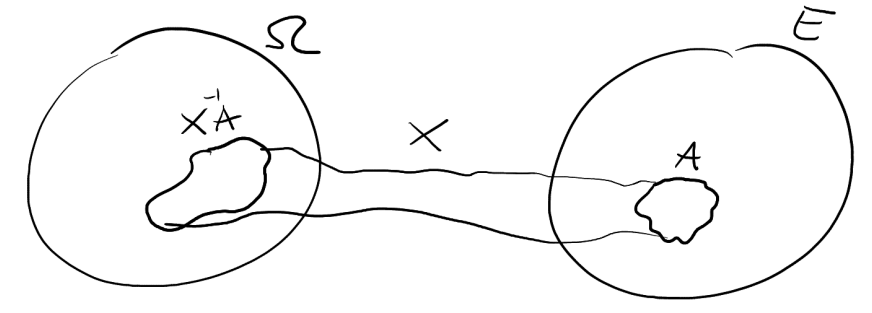
\includegraphics[width=0.8\linewidth]{screenshot001}
	\caption[References to suicide are to be taken seriously]{this is an early reminder of the fact that I will take my own life very soon.}
	\label{fig:screenshot001}
\end{figure}
So if $X^{-1}A$ is measurable by $\pr$ then it is in $\mathscr{H}$: otherwise it is not in $\mathscr{H}$. So \[\pr(X^{-1}A)=\pr\left(\left\{\omega\in\Omega:X(\omega)\in A\right\}\right).\] The message is that I am interested/able to evaluate $\pr$ over the set only if what I am evaluating is indeed an event (which means: it belongs to $\mathscr{H}$\footnote{il lettore più arguto avrà notato che, a questo punto, il dio è ormai irrimediabilmente cane.}). If something is not in $\mathscr{H}$ get it off my fucking face man and kill yourself NOW\footnote{
		
\includegraphics[width=0.05\linewidth]{screenshot002}
}. This is the only restriction for a random variable. $E$ can be whatever we need it to be: a graph, a tree, your mom being absolutely \censor{torn apart} by me. But most of the times, we have $E=\R$ or $E=\R^d$ with respectively $\mathscr{E}=\mathscr{B}\footnote{Borel \sa. You don't know what a Borel \sa\; is? \url{https://en.wikipedia.org/wiki/Borel_set}}(\R)=\mathscr{B}_\R$ and $\mathscr{B}_{\R^d}$.
\begin{remark}
	The simplest random variables are indicator functions of events.
	Example: take $H\in\mathscr{H}$. Define the function
	\begin{align*}
		\indi_H&:\Omega\rightarrow\R\\
		\indi_H(\omega)&=\begin{cases}
			0 &\omega\not\in H\\
			1 &\omega\in H
		\end{cases}
	\end{align*}
\end{remark}
\begin{remark}
	A random variable is said to be \enf{simple} if it takes only finitely many values in $\R^d$.
\end{remark}
\begin{remark}
	A random variable is said to be \enf{discrete} if it takes only countably many values.
\end{remark}
We are now ready to define the concept of \textit{distribution of a random variable}. But first...
\begin{figure}[H]
	\centering
	\begin{tikzpicture}
	\lemmethink[width=4.3cm,position={(-1,-1)},fill=white]{Yeah I don't know about you guys but I have the uncomfortable sensation that we are about to talk about distributions and I won't be able to see a goddamn integral like I am used to do. Can we address this fact please?}
\end{tikzpicture}
\end{figure}
Sure. Let's have a look back to Lebesgue integration.
\begin{tcolorbox}[enhanced jigsaw,sharp corners, drop fuzzy shadow=gray,colback=white,frame style={white},interior style={fill stretch image=lebe},width=\linewidth,height=0.27\linewidth]
\end{tcolorbox}
	\begin{revise}
		Consider a measure space $(E,\mathscr{E},\mu)$. $\E$ can be seen as the collection of all $\E$-measurable functions $f:E\mapsto\overline{\R}$ on $E$ that can be denoted with an abuse of notation\footnote{I am the only one being abused here.} by $f\in\E$ and by $d\in\E_+$ if the functions are positive. Our aim is to define integrals of measurable functions with respect to the measure $\mu$ so that:
		\[\mu f=\mu(f)=\int_E f(x)\mu(\dx)=\int_Ef\dif\mu\]
		which is written as the product of $\mu$ and $f$. It is interesting to note, in the last part of the equation, that the integral reads something like: "integrate $f$ over $E$ with respect to the measure $\mu$". What is this measure?? This is the question. Turns out that the good old Riemann integral is just a particular case of the Lebesgue integral when a certain measure is chosen.\\
		 We consider them as the generalization of vectors and hence the scalar product becomes a sum, which transforms into an integral. We will define the Lebesgue integral in three steps:
		\begin{enumerate}
			\item Simple and positive functions:
			\begin{definition}
			The function $f$ is called a \enf{simple and positive function} if it can be written as $$\sum_{i=1}^{n}a_i\indi_{A_i}$$ where $A_i\in\E$ and $a_i\geq0\in\R$ for $i=1,2,\ldots,n$.
			\end{definition}
			\begin{definition}
				For simple and positive functions, we define the Lebesgue integral as 
				\[\mu f:=\sum_{i=1}^{n}a_i\mu(A_i)\]
			\end{definition}
			\item Positive and measurable functions:
			\begin{theorem}
				Let $f\in\E_+$. Then there exists a sequence of simple and positive functions $f_n$ such that $f_n\nearrow f$.
			\end{theorem}
			Thanks to this theorem, we can well pose the following definition"
			\begin{definition}
				Let $f\in\E_+$. We define
				\[\mu f:=\lim_{n}\mu f_n\]
				where $f_n$ is a sequence of simple and positive functions such that  $f_n\nearrow f$.
			\end{definition}
			\item Recall a general fact for real-valued functions.
			\begin{remark}
				Let $f$ be a real-valued function. Then we can write
				\[f=f^+-f^-\]
				With $f^+:=f\vee0=max\{f,0\}$, called \emph{positive part} and $f^-:=-(f\wedge0)=-min\{f,0\}$, called \emph{negative part}. Both of them are real and positive functions and $f$ is measurable \underline{if and only if} $f^+$ and $f^-$ are real and positive functions.
			\end{remark}
		\end{enumerate}
		We are now ready to define the Lebesgue integral for measurable functions in $\R$. The trick is to separate the positive and the negative part of the function, to treat them as the limit of sequence of simple functions and then lose ourselves in the bliss of measure theory.
		\begin{definition}
			Let $f\in\E$. We define
			\[\mu f:=\mu(f^+)-\mu(f^-)\]
			Provided that \underline{at least} one of the integrals is finite in order to be defined and not incur into indefinite forms like $+\infty$ or $-\infty$.
		\end{definition}
		This definition can be easily converted if $f$ is a complex function: we only have to remember that we can decompose any complex number in its real and imaginary part. Both of them will be measurable real functions.
		\[f=\mathfrak{Re}^+f-\mathfrak{Re}^-f+i(\mathfrak{Im}^+f-\mathfrak{Im}^-f).\]
		From now on we will use this notation for the Lebesgue integral on $(E,\E)$:
		\[\mu f=\int_Ef(x)\mu(\dx)\qquad\text{with }f\in\E\]
		and if we choose $f=\indi_B$ with $B\in\E$. then
		\[\mu f=\mu \indi_B=\int_E\indi_B(x)\mu(\dx)=\indi_B\mu(\dx)=\mu(B).\]\par
		So this last equivalence helps us to understand one thing. \underline{Integrals are a device that needs a measure and a function to work}. In the notation above, $\dx$ has the meaning of an infinitesimal amount of the variable $x$ that is fed into the function $f$. Writing $\mu(\dx)$ means measuring an infinitesimal amount of $x$ using the measure $\mu$.\\
		In Riemann integration, $\dx$ represents an infinitesimal segment of the $x$-axis multiplied by the height of the function at $x$ (which is, of course, $f(x)$) and summed ($\int_{a}^{b}$) with all the other infinitesimal segments of the $x$-axis over the interval $[a,b]$. \\
		Here it's really the same thing with the difference that we multiply the height of the function $f(x)$ by calculating the "weight", or "\underline{measure}" of a smaller and smaller part of the domain that "causes that function to be of that height", according to our method of measure of choice. We do this over the set $E$.\par	
	\end{revise}
	\begin{tcolorbox}[enhanced jigsaw,sharp corners, drop fuzzy shadow=gray,colback=white,frame style={white},interior style={fill stretch image=lebe2},width=\linewidth,height=0.27\linewidth]
	\end{tcolorbox}
The main difference between Riemann and Lebesgue integration is, in a certain way, \textit{what} we are slicing. In the Riemann approach be basically do the following:
\begin{enumerate}
	\item slice the $x$-axis in smaller and smaller slices;
	\item compute $f(x)$;
	\item sum all the cute little rectangles you got.
\end{enumerate}
In the Lebesgue approach we basically \textit{start by choosing different slices of the }range\textit{of the function}, that is the co-domain. These little "slabs" of the range of the functions are nothing else but the "stepped" simple function version of our function:
\begin{figure}[H]
	\centering
	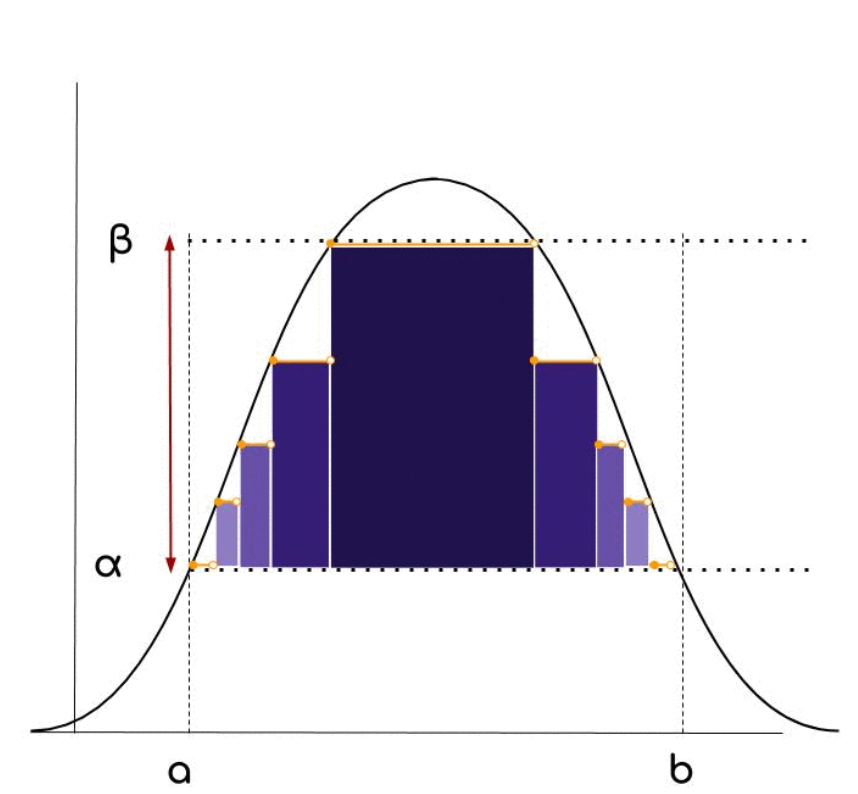
\includegraphics[width=0.46\linewidth]{screenshot004}
	\caption{Imagine the steps getting smaller and smaller...}
	\label{fig:screenshot004}
\end{figure}
Since we are dealing with simple functions, we are effectively approaching the problem from the $y$-axis. This means that since we are choosing slices of height \textit{first} our "slabs" may have different length when it comes to the $x$-axis. Anyway was it really SO DIFFICULT to explain? I don't think so. Fuck you mathematicians.\\
	So... will there ever be a measure and a set for which we will be able to circle back to our definition of Riemann integral? Hmm...\par
\begin{definition}
	\enf{Distribution of a random variable}. Let $X$ be a random variable taking values in $(E,\mathscr{E})$ and let $\mu$ be the image of $\pr$ under $X$, that is,
	\[\mu(A)=\pr(X^{-1}A)=\pr(X\in A)=\pr\circ X^{-1}(A)\footnote{you would know this if you knew fucking measure theory I guess},\;A\in\mathscr{E}.\] Then $\mu$ is a probability measure on $(E,\mathscr{E})$ and it is called \textbf{distribution of X}.
\end{definition}
So we map, by means of $X$, sets belonging to $\mathscr{E}$ into $\mathscr{H}$ and then evaluates this sets by means of the measure $\pr$. This is what we mean when we say that distributions are ultimately built with the probability measure and the random variable. \\
Distribution is itself a measure. To be exact it is a measure that we employ with a function (that in our case is a \rv{}) to form a Lebesgue integral just like we have seen in the revise box above. As we said, integrals are a machine that needs a function and a measure;
 in the case of probability theory these elements are respectively the \emph{random variable} and the \emph{probability distribution}.\\
 Right now we can start to see the light at the end of the tunnel\footnote{This is only the first chapter.} and start to have an intuition for all the ingredients to create this soup called "probability theory". Distributions are NOT cumulative density functions and neither they are probability density functions... They are something that transcends these "specialized" concepts and goes to the heart of how we evaluate (how we weigh; how we \textbf{measure}) a probability in a certain scenario. 
\begin{center}
	 Distributions are probability measures.
\end{center}
\begin{remark}
	You should remember (LOL) that when we want to specify a measure on a $\sigma$-algebra, it's enough to do it on a \textit{$\pi$-system}\footnote{a $\pi$-system is a simpler object than a $\sigma$-algebra: it is simply a collection of sets closed under intersection} generating that $\sigma$ algebra: by means of the monotone class theorem we are then able to extend the measure to the $\sigma$-algebra. \\
	This means that to specity $\mu$ it is enough to specify it on a \textit{$\pi$-system} which generates $\mathscr{E}$. For example, consider $E=\overline{\R}, \mathscr{E}=\mathscr{B}_{\overline{\R}}$. Consider the collection of sets $[-\infty,x],\;x\in\R$ which is of course a $\pi$-system because it is closed under intersection. Moreover, this shit generates the Borel sigma algebra on $\overline{\R}$. \\If we want to define a distribution, that is a measure, it is enough to define it on this $\pi$-system. Imagine that we apply our distribution measure to one set of this $\pi$-system
	\[c(x)\footnote{because it is a function of $x$}=\mu\left([-\infty,x]\right)=\pr(X\leq x),\qquad x\in\R\] by the monotone class theorem. So we have now specified the measure on the $\pi$-system. The part $\pr(X\leq x)$ reminds us of the undergraduate times\footnote{I already wanted to kill myself at that time.}: it is a distribution function! This is what our professor did implicitly to avoid using measure theory\footnote{I have noticed that my life has not benefited in ANY form since I have been introduced to measure theory.}.
\end{remark}
\begin{revise}
	But what is the \textit{monotone class Theorem}? First, we need the definition of \textit{monotone class}:
	\begin{definition}
		A collection of functions $\mathcal{M}$ is called \enf{monotone class} provided that:
		\begin{enumerate}
			\item it includes the constant function 1;
			\item taken $f$ and $g\in\mathcal{M}_b$ (with $\mathcal{M}_b$ being the subcollection of bounded functions in $\mathcal{M}$) and $a,b\in\R$, then $af+bg\in\mathcal{M}$;
			\item if the sequence $(f_n)_{_n}$ is contained in $\mathcal{M}_+$ (with $\mathcal{M}_+$ being the subcollection consisting of positive functions in $\mathcal{M}$) and $f_n\nearrow F$ then $f\in\mathcal{M}$.
		\end{enumerate}
	\end{definition}
	\begin{theorem}
		\enf{Monotone class Theorem}:\\
		Let $\mathcal{M}$ be a monotone class of functions on $E$. Suppose, for some $\pi$-system $\mathcal{C}$ generating $\mathscr{E}$, that $\indi_A\in\mathcal{C}$ for every $A\in\mathcal{C}$. Then $\mathcal{M}$ inclueds all positive $\E$-measurable functions and all bounded $\E$-measurable functions.
	\end{theorem}
\end{revise}
So, turning back to the previous remark: in that case $\E$ consists of the Borel \sa{} on the extended real line ($\B_{\overline{\R}}$); our $\pi$-system is capable of generating the Borel \sa{} (because every Borel set can be constructed with the combination $[-\infty,x]$ for all $x\in\R$\footnote{I know, I know: the fuck is a Borel set? A Borel set is every set that can be formed by the countable union or countable intersection or complementation from any open or closed set. You see that every Borel set you can imagine can be constructed by $[-\infty,x]$.}); we defined the measure $\mu$ on the $\pi$-system $[-\infty,x]$ for all $x\in\R$; the monotone class theorem states that if a class of sets (in this case, the class of sets where $\mu$ is well-defined) contains a $\pi$-system (\checkmark) and is closed under monotone limits (i.e. is a \underline{monotone class}), then it contains the $\sigma$-algebra generated by the $\pi$-system: this means that the class of sets where the distribution $\mu$ is well-defined will include the Borel \sa{} $\B_{\overline{\R}}$. This is kinda cool, I'll have to admit. Unfortunately, I don't really care about this.
\subsection{Functions of random variables}
Consider $X$, a random variable taking values in $(E,\mathscr{E})$ and consider further a measurable space $(F,\mathscr{F})$. Let $f:E\rightarrow F$ be a measurable function relative to $\mathscr{E}$ and $\mathscr{F}$\footnote{This basically means that this bitch won't do anything evil. The whole point of measure theory, $\sigma$ algebras and all other shit is to ensure everything behaves.}. This function should me measurable by means of $\pr$, otherwise we couldn't do anything useful with it. Consider the composition
\[Y=f\circ X\qquad\text{such that}\;Y(\omega)=f\circ X(\omega)=f\big(X(\omega)\big),\;\omega\in\Omega.\]
This composition is a random variable taking values in $(F,\mathscr{F})$ which comes from the fact that measurable functions of measurable functions are still measurable. 
\begin{definition}
	Consider two random variables $X,Y$ taking values in $(E,\mathscr{E})$ and $(F,\mathscr{F})$ respectively. Consider the pair
	\[Z=(X,Y):\Omega\rightarrow E\times F.\]
	Why would we want to call it $Z$? It's because, beside being a random vector, it is in turn a random variable:
	\[Z(\omega)=(X(\omega),Y(\omega)).\]
	Since $E\times F$ is a product space, we should attach it the product $\sigma$-algebra. So $Z$ is a random variable taking values in $E\times F$. 
\end{definition}
Note that the product space $E\times F$ is endowed with the \sa $\mathscr{E}\otimes\mathscr{F}$, that is the product \sa generated by the collection of all possible rectangles between $E$ and $F$. We frequently have to look to special cases like random vectors that must take values in measurable spaces for them to make sense. This measurable space is naturally generated by the product \sa (but it may be generated by other $\sigma$-algebras\footnote{Repeatedly inflicting painful kicks on my gonads.}!).
\begin{definition}
	We call \enf{joint distribution} of $X$ and $Y$ the distribution of $Z$. 
\end{definition}
This is interesting, since we know that this variable has the specific structure of a random vector: we identify the distribution of this vector as the joint distribution of its two coordinates\footnote{it eludes me how anyone could find this interesting. We have to think about the whole vector as being distributed like its components separately}. 
\begin{remark}
	The product \sa{} $\mathscr{E}\otimes\mathscr{F}$ is generated by the $\pi$-system of measurable rectangles.
\end{remark}
On the product space, it is enough to only specify it on this $\pi$-system.\par
Let denote with $\pi$ the joint distribution of $X,y$. It is sufficient to specify
\[\pi(A\times B)=\pr(X\in A, Y\in B)\qquad\every  A\in\mathscr{E},B\in\mathscr{F}.\]
We exploited the measurability of $X$ and $Y$
\begin{definition}
	Given the joint distribution $\pi$, consider sets $A\in\mathscr{E},B\in\mathscr{F}$. Then we call \enf{marginal distribution of $X$}
	\[\pr(X\in A)=\pi(A\times F)\qquad\;\every  A\in\mathscr{E}\]
	and we call \enf{marginal distribution of $Y$}
	\[\pr(Y\in B)=\pi(E\times B)\qquad\;\every  B\in\mathscr{F}.\]
\end{definition}
We call it distribution because it is actually a measure! So we can call it with the notation of measure
	\[\mu(A)=\pr(X\in A)=\pi(A\times F)\qquad\;\every  A\in\mathscr{E}\] and \[\nu(B)=\pr(Y\in B)=\pi(E\times B)\qquad\;\every  B\in\mathscr{F}.\]This actually means that the second coordinate is fixed in being the \underline{whole space} $F$. Think about integrating the second coordinate along the real line when doing marginal distributions... this is the same thing here.\\
Now that we have joint and marginal distributions, what is the next step\footnote{Abandoning myself in the sweet embrace of Death, methinks.}?
\begin{definition}
	Let $X,Y$ be \rv s taking values in $(E,\mathscr{E})$ and $(F,\mathscr{F})$ respectively and let $\mu$ and $\nu$ be their respective distributions. Then $X$ and $Y$ are said to be \enf{independent} if their joint distribution is the product measure formed by their marginals.
	\[\pr(X\in A,Y\in B)=\pr(X\in A)\pr(Y\in B)\qquad\every  A\in \mathscr{E},B\in\mathscr{F}.\]
	This also means that 
	\[\pi=\mu\nu\]
\end{definition}
Here the marginals do not interact with each other. This is true for two random variables but we need\footnote{No.} something more general.
\begin{definition}
Let $(X_1,X_2,\ldots,X_n)$ be a finite collection of random variables. The collection is said to be an \enf{independency} if the distribution of $(X_1,X_2,\ldots,X_n)$ is the product of $\mu_1,\mu_2,\ldots,\mu_n$ where $\mu_i$ is the distribution of $X_i$, for $i=1,\ldots,n$.
\end{definition}
Çinlar is stupid I wish him dead to be frank for this independecy shit. Independecy is not even an english word. What the fuck? Anyway, what about infinite collections?
\begin{definition}
	Let $(X_n)_{_n}$ be an infinite collection of \rv s. It is said to be an \enf{independency} if every finite sub-collection of it is an independecy.
\end{definition}
We now turn to stochastic processes\footnote{Please no.}! But first...
\subsection{Infinite product spaces}
Let $T$ be an arbitrary (countable or uncountable) set. We will think about this set as an "index" set. For each $t\in T$ consider the measurable $(E_t,\mathscr{E}_t)$. So we have a space for each index (plenty of measurable spaces hanging around). Consider a point $x_t$ in $E_t$ for each $t\in T$. The collection\footnote{We could consider it a function of $t$ but that wouldn't be exactly correct since each $t$ has a different measurable space. We may have the same space but it's not true in general... I am thrilled to say the least.} $(x_t)_{_{t\in T}}$. If  $(E_t,\mathscr{E}_t)=(E,\mathscr{E})$ then $(x_t)_{_{t\in T}}$ is actually a function of $T$ taking values on $(E,\mathscr{E})$. \\
The set $F$ of all possible functions $x=(x_t)_{_{t\in T}}$ is called the \enf{product space} $\left((E_t\mathscr{E}_t)\right)_{_{t\in T}}$.\\ This is the natural generalization of what we do when we construct product spaces, albeit with a different notation. Usually $F$ is denoted by $X_{t\in T}E_t$. But we know we also need a \sa...\\
A \enf{rectange} in $F$ is a subset of the form
\[\{x\in F:x_t\in A_t \;\every t\in T\}\]
Where $A_t$ differs from $E_t$ for only a finite number of $t$. So I want to consider subsets of $F$ (the space of functions) of the form above. I want only the functions $x$ in $F$ such that each coordinate belongs to $A_t$, a subset of $E_t$ for each $t\in T$. It seems that we have a restriction on all the coordinates... But this may bring to problems when we have an uncountable number of coordinates and therefore an uncountable number of restrictions. But we can says that if $A_t=E_t$ (the whole space) we don't apply any restriction. So in this case  $X_t$ belongs to $E_t$ so we can choose whatever $X_t$ we like. So only a finite number of coordinates are restricted while the other infinite ones are free to vary\footnote{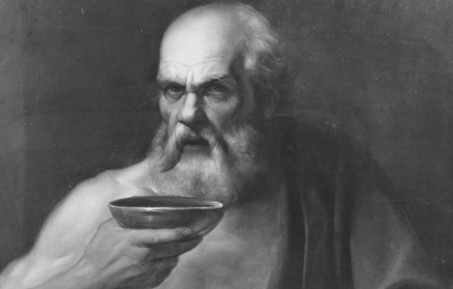
\includegraphics[width=0.08\linewidth]{screenshot003}$\rightarrow$ my honest reaction.
}. \par
The \sa{} generated by the collection of all measurable rectangles is denoted by 
\[\bigotimes_{t\in T}\mathscr{E}_t.\]
This is the product \sa{} in any infinite-dimensional space. So, the (natural) resulting measurable space in the end will be
\[\bigtimes_{t\in T}E_t,\bigotimes_{t\in T}\mathscr{E}_t.\] This is not in contrast with what we already know for finite product space, since these already have a finite number of restrictions. So this concept of rectangle, which can be a bit different from the one regarding the famous and well-tested geometrical shape\footnote{Oh thank god someone finally said it. I was starting to get scared.}, is not restricted on all the coordinates (like the shape\footnote{I swear to god.}) but only on a finite number of them. \\
We also have an alternative notation for this measurable space!
\[\bigotimes_{t\in T}(E_t,\mathscr{E}_t).\]
In the case that $(E_t,\mathscr{E}_t)=(E,\mathscr{E})\;\every t\in T$ the product space is denoted by
\[(E,\mathscr{E})^T\] or 
\[(E^T,\mathscr{E}^T)\]
These are not real powers but it's just notation... Anyway these are all different notations to indicate the infinite product space with the product \sa{} built upon the $\pi$-system which is the collection of all possible rectangle defined in the way we saw above\footnote{NO I WON'T USE LABELS AND NUMBERED EQUATIONS.}.
\subsection{Stochastic processes}
\begin{definition}
	Let $(E,\mathscr{E})$ be a measurable space and consider an index set $T$ (as before, an arbitrary set countable or uncountable).\\
	Let also $X_t$ be a \rv{} taking values in $(E,\mathscr{E})$. Then the collection of those random variables $(X_t)_{_{t\in T}}$ is called a \enf{stochastic process} with state space $(E,\mathscr{E})$ and parameter set $T$.
\end{definition}
Note that there is no mention about time here. Just think about the index set, which indexes the stochastic process. If we interpret $T$ as time then we have the most common interpretation of stochastic processes. But it could also be space (imagine $\R^2$) or your mom being \censor{fucked hard}. Anyway the most natural interpretation is time.\par
Now take a $\omega\in\Omega$ and evaluate all these \rv s on the same $\omega$. What we get is
\[t\mapsto X_t(\omega)\]
which is a function from $T$ to $(E,\mathscr{E})$. So if we see it as a function of $t$ for each $\omega$ we get a function which is an element of $E^T$. So what is a stochastic process, to sum it up? It's just a random variable taking values in the infinite product space $E^T$. That's why it is a problematic object: it's because mathematicians deserve to experience the sadness and evil they unleashed upon the world. Ever noticed how similar the words "measurable" and "miserable" are? I didn't think so. 
\begin{figure}
	\centering
	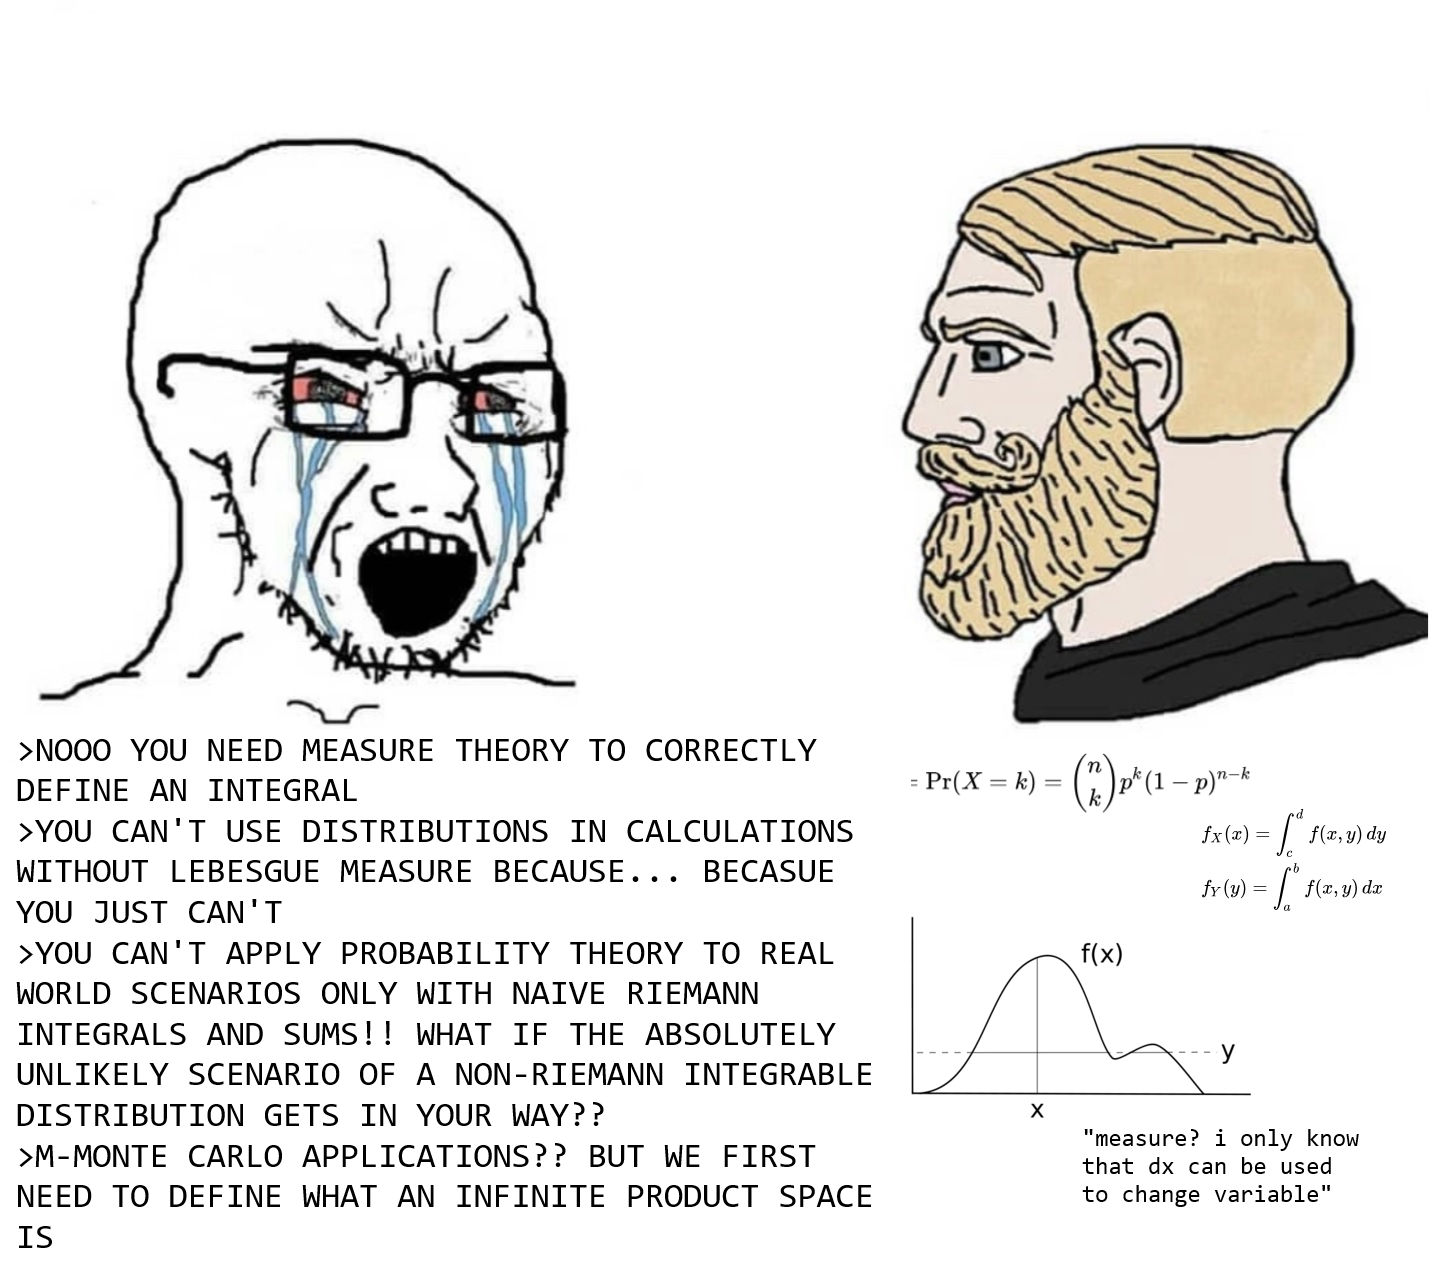
\includegraphics[width=0.7\linewidth]{ILMEMINO}
	\caption{I'm sorry but here you're the soyjack and I'm the chad.}
	\label{fig:ilmemino}
\end{figure}
Yeah technically more structure helps us modeling real phenomena more accurately but who the FUCK cares. 
\subsection{Example of random variables}
Consider some examples of simple random variables:
\begin{example}
	\enf{Poisson \rv s.}\\
	This \rv{} takes vales in $\N$ (it's a one dimensional \rv{}). We consider the power set of $\N$\footnote{Subset of all subsets of $\N$.}. We know that power sets \textit{are} \sa s that we can use (but we could encounter some trouble with uncountable elements, for which we would need smaller \sa s\footnote{No one really cares, not even Federico Polito.}).\\
	What is the distribution of this \rv{}?
	\begin{align*}
	\mu(A)=\pr(X\in A)&=\sum_{n\in A}\pr(X=n)\qquad A\subset\N\\
	\text{with } \pr(X=n)&=e^{-c}\frac{c^n}{n!}, \;n\in\N,\;c>0.
	\end{align*}
	So imagine we have this kind of random variable. We consider a subset of the natural number and we want to evaluate the measure of this subset that we chose. We know that we define the \rv{} by defining the distribution. For each $n$ we get a number $e^{-c}\frac{c^n}{n!}$. Another interesting implication is that \[\sum_{n\in A}\pr(X=n)=\sum_{n\in\N}\delta_n(A)\pr(X=n)\] where $\delta_n(A)$ is the \enf{Dirac measure} sitting at $n$. So, $n$ is a parameter and 
	\[\delta_n(A)=\begin{cases}
		1 &n\in A\\
		0 &n\not\in A
	\end{cases}.\] The Dirac measure is similar to the indicator function (they behave basically in the same way) but the difference is that this one is a \textit{measure} and the latter is a \textit{function}. The Dirac measure has $n$ as a parameter, while the indicator function has the set as a parameter ($\indi_A(n)$).
\end{example}
\begin{example}
	\enf{Exponential \rv{}}\\
	This random variable is again one-dimensional but this time this random variable is \textit{absolutely continuous}. What does it mean? It actually means that the variable is absolutely continuous with respect to the Lebesgue measure\footnote{'tacci tua.}. This is evident when we write down the distribution.\\
	Consider a \rv{} taking values in $\R_+$ and further consider $\mathscr{B}_{\R_+}$. We have
	\[\mu(\dif x)=\underbracket[0.6pt]{\dif x}_{\mathclap{Leb(\dif x)}}ce^{-cx},\qquad c>0,\;x\in\R_+.\]
	Ok no wait hold your fucking horses, cowboy. Why did we write $\dif x$ instead of just $x$? Also weren't densities, like, a fucking measure of some set in the form of $\mu(A)$? I like the fact that these densities resemble more closely the probability density function I was taught to work with during my sad Economics degree but there are many many things that creep me out. \par
	We have an answer for this, but we need to do a bit of backtracking.
\end{example}
	\begin{revise}
		First of all: what does "absolutely continuous" \textit{even means}?
		\begin{definition}
			let $\mu$ and $\nu$ be measures on a measurable space $(E,\mathscr{E})$. Then, measure $\nu$ is said to be absolutely continuous with respect to measure $\mu$ if, for every set $A\in\E$,
			\[\mu(A)=0\implies\nu(A)=0.\]
		\end{definition}
		Huh. That was pretty simple. Well, turns out we can exploit this fact to "switch" between different measures inside of integrals...
		\begin{theorem}
			\emph{Radon-Nikodyn Theorem}.
			Suppose that measure $\mu$ is $\sigma$-finite and measure $\nu$ is absolutely continuous with respect to $\mu$. Then there exists a positive $\E$-measurable function $p$ such that 
			\[\int_E\nu(\dx)f(x)=\int_E\mu(\dx)p(x)f(x)\qquad f\in\E_+.\]
			If we use the alternative notation:
			\[\int_Ef\dif\nu =\int_Ep f\dif\mu \qquad f\in\E_+.\]
			Moreover, $p$ is unique up to equivalence: if the equation above holds for another $\hat{p}\in\E_+$ then $\hat{p}(x)=p(x)$ for $\mu$-almost every\footnote{This means that all the setes where this condition doesn't hold are neglegible when weighted with measure $\mu$.} $x\in\E_+$. This is an if and only if statement!\par
			Also, $p$ is called the \emph{Radon-Nikodyn derivative} of $\nu$ with respect to $\mu$:
			\[\frac{\nu(\dx)}{\mu(dx)}=\frac{\dif\nu}{\dif\mu}=p.\]
		\end{theorem}
		With all this alternative notation this thing honestly feels like trying to understand the Metal Gear Solid plot, where identical characters named Snake keep cloning each other and being triple crossed by everyone until you finally understand that the storyline never made sense in the first place and that Hideo Kojima writes his games like a fucking fanfiction.
	\end{revise}
	Now everything should make more sense\footnote{Enviable optimism.}. If we know that a given \rv{} (say, the exponential random variable) has a distribution $\mu(\dx)$ then we will be able to transform this in a distribution of the form $\text{Lebesgue measure}\cdot p(x)$ (we can lose $f$ if $f$ is constant).
	In this formulation	$\dif x$ stands for the Lebesgue measure and the second part of the equation ($ce^{-cx}$) is the $p(x)$, called \emph{density function}. We can do this because we can see from the formula that this distribution, or measure, is indeed absolutely continuous with respect to the Lebesgue measure since we can express it in the form stated by the Radon-Nikodyn theorem.
	 So $p(x)=ce^{-cx},\;x\in\R_+$ is the density relative to $\mu$. This should serve us as a demonstration that if we define the \rv{} we get the distribution/measure (remember! distributions are measures!) and vice versa.

It is interesting\footnote{Debatable claim.} to see that also discrete random variable turns out to be absolutely continuous... But not with respect to the Lebesgue measure. To exact, discrete \rv s are absolutely continuous with respect to the \textit{counting} measure. And here's why to do all this shit we need the Lebesgue integral: by changing the measure we are using to compute the integral, we can use just one object (the probability distribution) to treat both discrete (using a counting measure, which gives us the cumulative distribution function in the form of a sum) and continuous \rv s (using the Lebesgue measure, which gives us the cumulative distribution function in the form of a Riemann integral.)

\vspace{0.5cm}
\begin{figure}[H]
\hspace{1.5cm}
\begin{tikzpicture}
	\calloutquote[width=5cm,position={(-1,-1)},fill=DodgerBlue4,rounded corners]{\color{white}So you know what a Lebesgue measure is, right?}
\end{tikzpicture} 
\begin{flushright}
	\begin{tikzpicture}
		\calloutquote[width=4cm,position={(1,-1)},fill=Turquoise4!30,rounded corners]{Of course not! Is that a bad thing?}
	\end{tikzpicture}\hspace*{2.5cm}
\end{flushright}
\hspace{2cm}
\begin{tikzpicture}
	\calloutquote[width=3cm,position={(-1,-1)},fill=DodgerBlue4,rounded corners]{\color{white}You were adopted}
\end{tikzpicture}
\caption{Actual conversation happened between me and Professor Lods.}
\end{figure}
So we're due for a little refresh on what the hell a Lebesgue measure is. I'm sorry\footnote{Not really. I mean, I'm sorry for the fact that they \textit{are} mathematicians but that's where my compassion starts and ends.} for our mathematician friends but I need this to be written loud and clear. This is from Professor Lods' Lecture notes from the pre-course in Measure Theory, with the hope that one day I'll be skilled like he is with \LaTeX{} typesetting.
\begin{revise}
Let's have a quick refresh about the Lebesgue measure over the measurable space $(\R,\mathscr{B}_{\R})$. Let $S=\R$. First of all, what is an algebra?
\begin{definition}
	A collection $\Sigma_0$ of subsets of $S$ is called an algebra on $S$ if:
	\begin{itemize}
		\item $S\in\Sigma_0$;
		\item if $A\in\Sigma_0$ then $A^c\in\Sigma_0$ where $A^c=S\setminus A$ is the complementary of $A$;
		\item if $A,B\in\Sigma_0$ then $A\cup B\in\Sigma_0$.
	\end{itemize}
\end{definition}
We also need the concept of pre-measure, which is basically a measure but defined on an algebra (instead of a \sa{}):
\begin{definition}
	Let $\Sigma_0$ be an algebra on $S$ (not necessarily a \sa{}. A mapping $\ell:\Sigma_0\mapsto[0,\infty]$ is said to be a \enf{pre-measure} on $\Sigma_0$ if $\ell(\emptyset)=0$ and for any pairwise disjoints $\{A_n\}_{_n}\subset\Sigma_0$ with $\bigcup_nA_n\in\Sigma_0$ it holds:
	\[\ell\left(\bigcup_{n=1}^\infty A_n\right)=\sum_{n=1}^{\infty}\ell{A_n}.  \] 
	Moreover, a pre-measure $\ell$ is said to be $\sigma$-finite on $\Sigma_0$ if there exists a sequence $\{A_n\}_{_n}\subset\Sigma_0$ with $\bigcup_nA_n\in\Sigma_0$ and $\ell(A_n)<\infty$ for any $n\in\N$.
\end{definition}
We can immediately see that $\bigcup_nA_n\in\Sigma_0$ is an additional assumption: in \sa s this assumption is always met. So if $\Sigma_0$ is a \sa{} any measure on $\Sigma_0$ is a pre-measure. \\
We also need one more thing: the \enf{Caratheodory's extension Theorem}.
\begin{theorem}
	\enf{Charatheodory's extension Theorem}: Let $S$ be a given set and let $\Sigma_0$ be an algebra on $S$ and $\Sigma=\sigma(\Sigma_0)$. If $\ell:\Sigma_0\mapsto[0,\infty]$ is a pre-measure on $(S,\Sigma_0)$ then there exists a measure $\mu$ on $(S,\Sigma)$ such that
	\[ \mu(A)=\ell(A)\qquad \every A \in \Sigma_0. \]
	Moreover, if $\ell$ is a $\sigma$-finite pre-measure on $\Sigma_0$, then such a measure $\mu$ on $(S,\Sigma)$ is unique and $\sigma$-finite.
\end{theorem}Apparently this is one of the principal results in measure theory since it allows to construct measures well-adapted to practical situations: once such measures are constructed, Caratheodory's theorem can go fuck itself off. But the most important question is: why do we care about these total nerds?
Because we can now define
\[\mathcal{C}_0=\{[a,b):-\infty\leq a\leq b\leq\infty\in\R\}\]
and let
\[ \Sigma_0=\left\{\bigcup_{j=1}^N I-J:I_j\in\mathcal{C}_0\;\every j,I_i\cap I_j=\emptyset\text{ if }i\neq j,N\in\N \right\} \]
We can prove without major difficulty that $\Sigma_0$ is an algebra on $\R$. Let's define a pre-measure on $\Sigma_0$ by setting:
\begin{itemize}
	\item $\ell([a,b))=b-a$ for any $b\geq a$;
	\item $\ell((-\infty,b))=\ell((a,\infty))=\ell(\R)=+\infty$;
	\item $\ell\left(\bigcup_{j=1}^N I_j\right)=\sum_{j=1}^{N}\ell(I_j)$ if $\{I_j\}_{_{j=1,\ldots,N}}\subset\mathcal{C}_0$ are pairwise disjoints.
\end{itemize}
It can be checked that this newly defined measure is $\sigma$-finite
Remember that $\sigma(\Sigma_0)=\sigma(\mathcal{C}_0)=\mathscr{B}_\R$, which is the Borel \sa{}. 
Consider, additionally, the result of the Charatheodory's extension Theorem. By stitching all of these amenities together we get:
\begin{theorem}
	There exists a unique measure  on $(\R,\mathscr{B}(\R))$ that we denote $\lambda$ (or $\mathfrak{m}$) and such that
	\[\lambda([a,b))=b-a\qquad\every a<b.\]
	We call this measure the \enf{Lebesgue measure} on $(\R,\mathscr{B}(\R))$.
\end{theorem}
\begin{flushright}
	\begin{tikzpicture}
		\calloutquote[width=6cm,position={(1,-1)},fill=white,rounded corners]{So we just learnt how to FIND A FUCKING INTERVAL ON THE REAL LINE?}
	\end{tikzpicture}\hspace*{1.5cm}
\end{flushright}
\hspace{2cm}
\begin{tikzpicture}
	\calloutquote[width=7cm,position={(-1,-1)},fill=DodgerBlue4,rounded corners]{\color{white}Look, I know that can be seen as useless formalism. And indeed it is! We just formalized the notion of \textit{length}. If we take it to 2-dimensional spaces we end up with the notion of area, in 3-dimensional spaces is the notion of volume... and so on.}
\end{tikzpicture}
\begin{flushright}
	\begin{tikzpicture}
		\calloutquote[width=6cm,position={(1,-1)},fill=white,rounded corners]{Huh. This makes sense. So this is the notion of volume when everything, including the real line, is a set. Kinda seems like the solution to a problem we ourselves created...}
	\end{tikzpicture}\hspace*{1.5cm}
\end{flushright}
\hspace{2cm}
\begin{tikzpicture}
	\calloutquote[width=4cm,position={(-1,-1)},fill=DodgerBlue4,rounded corners]{\begin{center}
			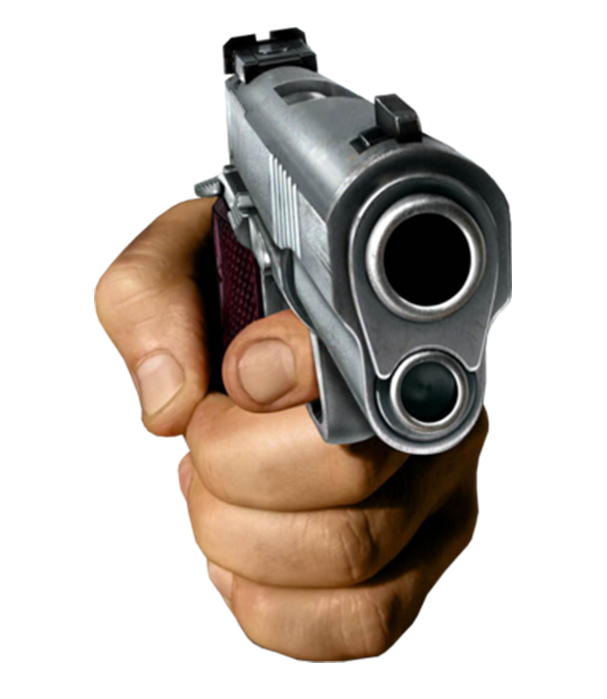
\includegraphics[width=0.5\linewidth]{lool}
	\end{center}}
\end{tikzpicture}
\begin{remark}
	We can define in the same way the Lebesgue measure on $(I, \mathscr{B}_I)$ for all $I\subset\R$.
\end{remark}
\begin{remark}
	The measure space $(\R,\mathscr{B}_\R,\lambda)$ is $\sigma$-finite since $([-n,n))_n\nearrow\R$ but is not finite since
	\[ \lambda(\R)=\lim_{n}\lambda([-n,n))=\lim_{n}2n=\infty\]
\end{remark}
\end{revise}
Yeah, that mysterious measure I was talking about before to connect Riemann and Lebesgue integration was the Lebesgue measure. We often just write $\dx$ to express the Lebesgue measure (which is what we did on example 1.2 about the exponential random variable), but the meaning is always the same, with a striking similarity to the concept of Riemann integration: take the Lebesgue measure of a smaller and smaller element of our $\B_{\overline{\R}}$ set, use it to "weight" (read: multiply) the value of the function for that element and then  sum it all up together. What we end up with is basically a serie of simple functions that slice "horizontally" the co-domain of the function. Keep reducing the size and you end up with the Lebesgue integral. Of course, when the measure is the Lebesgue measure, the Riemann and the Lebesgue integral have a really similar interpretation.\par
Back to our topic: the exponential \rv{} is absolutely continuous with respect to the Lebesgue measure.  
It is interesting to see that also discrete \rv s turn out to be absolutely continuous: the difference is that they are not absolutely continuous to the Lebesgue measure, but the \textit{counting} measure. At the undergrad level we are used to say that a \rv{} is either discrete or absolutely continuous, buy this was ultimately a lie\footnote{Measure theory turns truths into lies. Truly a demonic machinery.}.
\begin{example}
	\enf{Gamma distribution}\footnote{She factorials on my $\gamma$ 'till I $\beta$.}:
	Consider a \rv{} taking values in $\R_+$ and consider as a \sa{} the Borel \sa{} $\mathscr{B}_{\R_+}$. The distribution of the Gamma \rv{} is the following:
	\[\mu(\dif x)=\dif x\frac{c^ax^{a-1}e^{-cx}}{\Gamma(a)},\qquad
	\text{with }
	\begin{array}{l}
		a>0,\\
		c>0,\\
		x\in\R_+
	\end{array}.\]
	Here $\Gamma(a)$ is the \textit{Gamma function:}
	\[
	\Gamma(a)=\int_{0}^{+\infty}e^{-x}x^{a-1}\dx.
	\]
	The Gamma function is one of the most famous special functions that comes up almost everywhere. This definition of Gamma function is valid just for positive values and can be seen as a \textit{Laplace transform}\footnote{$\mathcal{L}\{f\}(s)=\int_{0}^{+\infty}f(t)e^{st}\dif t$ where s is a complex number $s=a+ib$.} or as a \textit{Mellin transform}\footnote{$\mathcal{M}[f;s]\equiv F(s)=\int_{0}^{+\infty}f(t)t^{s-1}\dt$ where $s=a+ib$.}.
	The first parameter $a$ is called \textit{shape parameter}; the parameter $c$ is called \textit{scale parameter}. This distribution is also continuous with respect to the Lebesgue measure. \par
	We have some special cases of the Gamma distribution but Federico Polito doesn't really care about. Just know that the $\chi^2$ distribution is a special case of the Gamma \rv{}.
\end{example}
\begin{example}
	This is a certified hood classic: \emph{Gaussian distribution}.\\
	Consider a \rv{} takinv values in $\R$. Of course we consider $\B_{\overline{\R}}$ and the distribution is (notice how also this one is absolutely continuous with respect to the Lebesgue measure):
	\[\mu(\dx)=\dx\cdot\underbracket[0.6pt]{\frac{1}{\sqrt{2\pi b}}e^{-\frac{(x-1)}{2b}}}_{\mathclap{p(x)}},\qquad \begin{array}{l}
	a\in\R,\\
	b>0\in\R,\\
	x\in\R_+
	\end{array}.\]
	Of course, $a$ is called the \textit{mean} of the distribution and $b$ is called the \textit{variance}.
\end{example}
\begin{example}
	This is a random variable that stems from two independent random variables having Gamma distribution. Consider $\gamma_a$ (distribution of a Gamma \rv{} with parameters $a$ and $c=1$) and $\gamma_b$ (distribution of a Gamma \rv{} with parameters $b$ and $c=1$). So, two gammas with different shape parameter. \\
	Let $X\sim\gamma_a$ and $Y\sim\gamma_b$. Moreover, let them be independent. This is a random vector $(X,Y)$ with two components... What is its distribution?
	\[\pi(\dx,\dy)=\underbracket[0.6pt]{\gamma_a(\dx)\cdot\gamma_b(\dy)}_{\mathclap{\text{because of independency}}}=\dx\dy\frac{e^{-x}x^{a-1}}{\Gamma(a)}\cdot\frac{e^{-y}y^{b-1}}{\Gamma(b)}.\]
	So it's easy to build joint distributions when the \rv s are independent\footnote{Well no shit. Even I can multiply two numbers}.
\end{example}
\begin{example}
	\emph{Gaussian \rv{} with exponential variance}.\\
	Here the variance is random and is distributed exponentially\footnote{because humans should never have the hubris to meddle with the horrorific world of random necessities that the Gods have laid before us.}. Consider a \rv{} $X$ taking values in $\R_+$ and a \rv{} $Y$ taking values in $\R$.\\
	Here we are again in presence of a random vector. The distribution is the following:
	\[\pi(\dx,\dy)=\dx\dy\cdot ce^{-cx}\frac{1}{\sqrt{2\pi x}}e^{-\frac{y^2}{2x}}\qquad \begin{array}{l}
		x\in\R_+,\\
		y\in\R
	\end{array}. \]
	\begin{remark}
		$\pi$ in this case has a special form: it has the form 
		\[\pi(\dx,\dy)=\mu(\dx)K(x,\dy).\]
		In particular, here $\color{Cyan4}\mu(\dx)$ is 
		\[\color{Cyan4}\dx\color{black}\dy\cdot\color{Cyan4} ce^{-cx}\color{black}\frac{1}{\sqrt{2\pi x}}e^{-\frac{y^2}{2x}},\]
		which is a docile exponential function, and $\color{Magenta4}K(x,\dy)$ is
		\[\color{black}\dx\color{Magenta4}\dy\cdot\color{black} ce^{-cx}\color{Magenta4}\frac{1}{\sqrt{2\pi x}}e^{-\frac{y^2}{2x}}.\]
		In this case $K(x,\dy)$ cannot be the distribution fo $Y$, because it has some $x$ in it. So this distribution is not simply the product of marginal distribution. But let's take a closer look to the form $\mu(\dx)K(x,\dy)$. $\mu(\dx)$ is certainly a measure, but what about $K(x,\dy)$? \par
	\end{remark}
\end{example}
\section{Transition kernels}
Turns out that $K(x,\dy)$, depending on $x$, is connected to the other measure $\mu(\dx)$. \\
The object $K(x,\dy)$ is called \emph{transition kernel}\footnote{Kernel? Colonel? I thought we were over with the Metal Gear Solid jokes.} and it's very important. Not that here 
$K(x,\dy)$ has the form 	
\[B\mapsto K(x,B)\]
It should be seen as a set function. Why? Just look back to $\pi(\dx,\dy)$. It is in differential form, but if we integrate the joint distribution against one set in the product space we get $\pi$ evaluated on that subset of the product function (it is a measure... measures are always set functions). So also $\mu(\dx)K(x,\dy)$ should be a set function. $\mu(\dx)$ is of course a set function (it is a measure...\footnote{All this passive-aggressiveness for what?}) and so should be $K(x,\dy)$. The presence of $x$ in $K(x,\dy)$ is what "links" the $X$ coordinate with the $Y$ coordinate of the random vector.
The Gamma example was about two independent random variables: here it is impossible to obtain the product of measures. Transition kernels are incredibly important because they are ultimately connected with the \textit{structure of dependency} between random variables: that's why this course is going to bust our ball into the oblivion about them\footnote{Professor Polito jokes that every year people complain about the abstractness of kernels and laughs about it. I'm happy that his sense of humor has been left untouched by my slightly scathing EDUMETER review of this course.}.
\begin{figure}[H]
	\centering
	
\includegraphics[width=0.57\linewidth]{codec}
	\caption[Colonel Campbell embraces her true self]{Yeah, no more Metal Gear Solid jokes after this one. I promise\protect\footnotemark.}
	\label{fig:codec}
\end{figure}
\footnotetext{This is not, in fact, the last Metal Gear Solid joke.}
Remember in the undergraduate courses: when there was dependence we usually expressed it with the \textit{conditional probability}. \\
Transition kernels let us manage random vectors that are not trivial and that have a dependence relationship with other random vectors. \\
Think about the previous example: the marginal distribution $\nu$ of $Y$ has the form \begin{align*}
	\nu(B)&=\pi(\R_+\times B)=\int_{\R_+}\mu(\dx)K(x,B),\qquad B\in\B_{\overline{\R}}\\
	&=\int_{\R_+\times B}\pi(\dx,\dy)=\int_{\R_+\times B}\dx\dy\cdot ce^{-cx}\frac{1}{\sqrt{2\pi x}}e^{-\frac{y^2}{2x}}\\
	&=\int_B \dy\; n(y),\qquad\text{where }n(y)=\int_{0}^{\infty}\dx \cdot ce^{-cx}\frac{1}{\sqrt{2\pi x}}e^{-\frac{y^2}{2x}}.
\end{align*}
So we have that the marginal distribution $\nu(B)$ is written as $\int_B \dy\;n(y)$ and is therefore absolutely continuous with respect to the Lebesgue measure. We could actually solve this integral ($n(y)$ is a closed form called \textit{two-sided exponent}). So we now have the marginal of $Y$ and the marginal of $X$ and we immediately realize that if we multiply the two densities we do not obtain the joint density (because they are dependent\footnote{OK I GET IT.}).\par
So we are now ready to define the concept of transition kernel.
\begin{definition}
	Let $(E,\E)$ and $(F,\F)$ be measurable spaces. Let $K$ be a mapping from $E\times\F$ into $\overline{\R}_+$. Then $K$ is called \emph{transition kernel} from space $(E,\E)$ into space $(F,\F)$ if:
	\begin{itemize}
		\item the mapping $x\mapsto K(x,B)$ is $\E$-measurable $\every B\in\F$;
		\item the mapping $B\mapsto K(x,B)$ (the second mapping of the kernel, the one regarding the set) is a measure $\every x\in E$.
	\end{itemize}
\end{definition}
We can consider the transition kernel a hybrid object: if we look at it with respect to the first variable it is a \textit{measurable function}, if we look at it with respect to the second variable it is a \textit{measure}.
\begin{example}
	Take $\nu$, a finite measure on $(F,\F)$ and take $k$, a positive function on $(E\times F)$ which is measurable with respect to $\E\otimes\F$, the product \sa{}. Then, we integrate
	\[\int_B\nu(\dy)k(x,y)\qquad\begin{array}{l}
		B\in\F\\
		x\in E
	\end{array}\]
	We see how this object depends on $x$ and on the choice of $B$ (a function of $x$ and $B$...). It defines a transition kernel
	\[K(x,B)=\int_B\nu(\dy)k(x,y)\qquad\begin{array}{l}
		B\in\F\\
		x\in E
	\end{array}\]
	from $(E,\E)$ into $(F,|F)$.
\end{example}
\begin{theorem}
	This theorem tells us what we can do with a kernel. Let $K$ be a transition kernel from $(E,\E)$ into $(F,\F)$. Then, 
	\begin{enumerate}[\circnum]
		\item we have $$\int_F K(k,\dy)f(y)\qquad \text{ with } x\in E,\;f\in\F_+.$$ This operation defines a function $Kf\in\E_+\;\every f\in\F_+$.
		
			\begin{notation}
			The notation $f\in\F_+$ in Çinlar is either the \sa{} $\F$ or the set of functions measurable with respect to the \sa{} $\F$. Another one of the many ways Çinlar chooses to sadden my day. But my revenge is on the way.
		\end{notation}
		 First of all we integrate the kernel with respect to the second variable (which basically means we use it as a measure on $F$). The integrand is $F$ and since this function is a measure with respect to the second variable I can integrate $\F_+$-measurable functions. Remember that $\mu f=\mu(f)=\int_E f(x)\mu(\dx)=\int_Ef\dif\mu$. \\
		The integration over $F$ "takes out" one part of the kernel from the equation (the measure part) so that we can write: \[
	Kf(x)=\int_F K(k,\dy)f(y);
	\]
	\item we want to use the kernel with respect to the first variable (obtaining a $\E$-measurable function), so we integrate 
	\[
	\int_E \mu(\dx)K(x,B)
	\]
	Remember that we must integrate the kernel with respect to a measure $\mu$ that is attached to the space $(E,\E)$. This operation (since we remove the "function" part of the kernel) defines a \textit{measure} $\mu K$ on $(F,\F)$ for each measure $\mu$ on $(E,\E)$ and we can write:
	\[\mu K(B)=	\int_E \mu(\dx)K(x,B);\]
	\item now we want to integrate everything: we consider the measure $\mu K$, take $f$ and calculate its integral with respect to the measure $\mu K$
	\[(\mu K)f.\]
	With $f\in\F_+$. We can now link the function obtained in step 1 and the measure obtained in step 2:
	\[(\mu K)f=\mu(Kf)=\int_E\mu(\dx)\cdot\int_FK(x,\dy)f(y)\]
for every choice of measure $\mu$ on $(E,\E)$ and for every choice of $f\in\F_+$
	
	
	\end{enumerate} 
\end{theorem}
	Remember that here $(\mu K)f$ is shortened notation: $\mu f$ means $\int_Ef(x)\mu(\dx).$ We are NOT applying the measure to the function!\\
Right... but if we choose $f\in\E$ ($f$ is $\E$-measurable) as the indicator function $f=\indi_B,\quad B\in \E$ (the most simple example of $\E$-measurable function), this happens:
\begin{align*}
	\mu\indi_B&=\int_E\indi_B(x)\mu(\dx)\\
	&=\int_B\mu(\dx)=\mu(B)
\end{align*}
This is the reason behind this kind of notation that switches between measures and integrals. This is interesting and useful, if "interesting and useful" was slang for "boring and useless". So technically yeah, we \textit{are} applying the measure to the function in the sense that we are weighing the function with the measure $\mu$. 
\begin{fancyproof}
	\begin{enumerate}
		\item[1] First of all, remember that $Kf$ resulting from the integral is a well defined function but that is not enough: we need a $\E$-measurable function of $K f$. We need to proceed in a constructive way: we have to think about $\E$-measurable functions, in whose space there are different type of functions: indicators, simple function, positive functions, positive or negative function. We start from simple function and then extend this result to positive functions and then to a broader class.\\
		First consider $f$ to be a simple function with its canonical representation:
		\[
		f=\sum_{i=1}^{n}b_i\indi_{B_i}
		\]
		for given weights $b_i$ and given sets $B_i$. For this function we consider
		\[Kf(x)=\sum_{i=1}^{n}b_i\underbrace{K(x,B_i)}_{\mathclap{\substack{\E\text{-measurable}\\ \text{with respect to }x}}}.\]
		So it is a linear combination of $\E$-measurable functions and therefore $K f\in\E_+$ when $f$ is simple. \par
		We now want to extend the proof to the subclass of positive measurable functions. Take $f$ positive. We know that we can approximate positive functions by means of simple functions, but reducing the "step" of the simple functions (discretizing the original function) by means of an auxiliary function called \emph{dyadic function} (see below), thus producing a sequence of simple functions. So we have
		$f\in\F_+$ and $f_n=\mathcal{d}_n\circ f$. \begin{lemma}
			Each $\dyadic_n$ is an increasing right-continuous simple function on $\overline{\R}_+$ and $\dyadic_n(r)$ increases to $r\;\every r\in\overline{\R}_+$ as $n\to\infty$.
		\end{lemma}
		So as soon as $n$ goes to infinity we get the original function. Moreover, remember the theorem that gives measurability of a function:
		\begin{revise}
			\begin{theorem}
				A positive function on $(E,\E)$ is $\E$-measurable if and only if it is the limit of an increasing sequence of positive simple functions.
			\end{theorem}
			\begin{theorem}
				Let ${(f_n)}_{n}$ be a sequence of positive measurable functions in $(S,\Sigma)$ with respect to a measure $\Sigma$ such that $f_n\nearrow f$ almost everywhere on the set $S$, Then 
				\[\lim_{n}\int_S f_n\dmu=\int_{S}^{}f\dmu\]
				where the sequence ${(\int_S f_n \dmu)}_{n}$ is a nondecreasing sequence.
			\end{theorem}
		\end{revise}
		We consider, as we said before, the discretization
		\[f_n=\dyadic_n\circ f.\]
		What happens to $K f(x)$? In this case, it is defined as:
		\[Kf(x)=\lim_{n\to\infty}K f_n(x)\qquad\every x\]
		and this is true for the monotone convergence theorem for the measure $B\mapsto K(x,B)$. Then $Kf$ is $\E$-measurable being the limit of the $\E$-measurable sequence of functions $(Kf_n)_n$.
		\item[2--3] Fix a measure $\mu$ on $(E,\E)$ and define a functional 
		\[L:\F_+\mapsto\overline{\R}_+\]
		by setting 
		\[L(f)=\mu(Kf)\]
		that is, we integrate $Kf$ with respect to the measure $\mu$. We note that
		\begin{enumerate}[i.)]
			\item\label{ite:frs} if $f=0$ then $L(f)=0$;
			\item\label{ite:scn} if $f,g\in\F_+$ with $a,b\in\R_+$ then 
			\begin{align*}
				L(af+bg)&=\mu\big(K(af+bg)\big)\\
				&=a\mu(Kf)+n\mu(Kg)\\
				&=aL(f)+bL(g).
			\end{align*}
			So the functional is a linear function.
			\item\label{ite:thr} if $(f_n)_{_{n}}\subset\F_+$ and $f_{n}\nearrow f$ then  $Kf_n\nearrow Kf$ and this is true by monotone convergence theorem with respect to integrals with respect to the measure $B\mapsto K(x, B)$. 
			\item\label{ite:frt} note that 
			\[L(f_n)=\mu(Kf_n)\nearrow\mu(Kf)\]
			again because of the monotone convergence theorem with respect to the measure $\mu$.
		\end{enumerate}
		So given that \ref{ite:frs}, \ref{ite:scn}, \ref{ite:thr} and \ref{ite:frt} hold (and recurring to the theorem 4.21 of the Cinlar book\footnote{yeah not gonna check that.}) we have that there exists a measure $\nu$ on $(F,\F)$ such that
		\[L(f)=\nu f\qquad \every f\in\F_+,\]
	
	\end{enumerate}
		Note that if we specifically take the function $f=\indi_B,\;B\in\F$ we see that 
	\begin{align*}
		\nu(B)=\nu\indi_B=L(\indi_B)&=\mu(K\indi_B)=\mu\left(\int_BK(x,\dy)\right)\\
		&=\mu K(x,B)=\int_EK(x,B)\mu\dx=\mu K(B).
	\end{align*}
	Then $\nu\equiv \mu K$, that is $\mu K$ is a measure on $(F,\F)$ and 
	\[(\mu K)f=\nu f=L(f)=\mu (K f).\] 
\end{fancyproof}
\begin{definition}
	The \emph{dyadic function} is defined as:
	\[
	\dyadic_n(r)=\sum_{k=1}^{n\cdot2^n}\frac{k-1}{2^n}\indi_{\left[\frac{k-1}{2^n},\frac{k}{2^n}\right)}(r)+n\indi_{\left[n,+\infty\right)}(r),\qquad r\in\overline{\R}_+
	\]
	So we basically have two different sections in this function: after $n$ the value of this function is equal to $n$, otherwise it is a step function in the sequence of interval from the start to $n$. To see the shape of this function we could see some examples.
\end{definition}
\begin{example}
	Take $n=1$. We can calculate this dyadic function obtaining
	\begin{align*}
		\dyadic_1(r)&=0,\qquad r\in\left[0,\frac{1}{2}\right)\\
		\dyadic_1(r)&=\frac{1}{2},\qquad r\in\left[\frac{1}{2},1\right)\\
		\dyadic_1(r)&=1,\qquad r\geq1.\\
	\end{align*}
	The function is right-continuos and a step function.
\end{example}
\begin{example}
	$n=1$. Try to do it by hand.
	\begin{align*}
		\dyadic_2(r)&=0,\qquad r\in\left[0,\frac{1}{4}\right)\\
		\dyadic_2(r)&=\frac{1}{4},\qquad r\in\left[\frac{1}{4},\frac{1}{2}\right)\\
		\dyadic_2(r)&=\frac{1}{2},\qquad r\in\left[\frac{1}{2},\frac{3}{4}\right)\\
		\dyadic_2(r)&=\frac{3}{4},\qquad r\in\left[\frac{3}{4},1\right)\\
		\dyadic_2(r)&=1,\qquad r\in\left[1,\frac{5}{4}\right)\\
		\dyadic_2(r)&=\frac{5}{4},\qquad r\in\left[\frac{5}{4},\frac{3}{2}\right)\\
		\dyadic_2(r)&=\frac{3}{2},\qquad r\in\left[\frac{3}{2},\frac{7}{4}\right)\\
		\dyadic_2(r)&=\frac{7}{4},\qquad r\in\left[\frac{7}{4},2\right)\\
		\dyadic_2(r)&=2,\qquad r\geq 2.
	\end{align*}
\end{example}
\subsection{Products of kernels}
Let $K$ be a kernel from $(E,\E)$ into $(F,\F)$ and let $K$ be a kernel from $(F,\F)$ into $(G,\G)$.
\begin{definition}
	The product of $K$ and $L$ is the transition kernel from $(E,\E)$ into $(G,\G)$ such that $(KL)f=K(LF)$ for $f\in\G_+$.
\end{definition}
Let's now fill in some information for transition kernels.
\begin{definition}
	A transition kernel from $(E,\E)$ into $(E,\E)$ is actually called \emph{transition kernel on $(E,\E)$}.
\end{definition}
This is actually the most common transition kernel in probability\footnote{Oh right we are studying probability theory. Thanks for reminding!}, since \rv s take values in the same space.
\begin{definition}
	A transition kernel on $(E,\E)$ is called \emph{Markov kernel} if 
	\[K(x,E)=1\qquad\every x\in E.\]
	It is called \emph{sub-Markov} if
	\[K(x,E)\leq1\qquad\every x\in E.\]
\end{definition}
So here we are, we summoned Markov for the first time in this course.
\begin{figure}[H]
	\centering
	
\includegraphics[width=0.4\linewidth]{markov}
	\caption{Andrej Andreevič Markov if he was cool.}
	\label{fig:markov}
\end{figure}
\begin{definition}
	Given a transition kernel on $(E,\E)$ its \emph{powers} are define recursively as follows:
	\begin{align*}
		K^0&=I\\
		K^1&=K\\
		&\vdots\\
		K^n&=K\cdot K^{n-1}
	\end{align*}
	$I$ is the identity kernel, i.e. $I(x,A)=\delta_x(A)=\indi_A(x)\quad\every x\in E,\, A\in\E$
\end{definition}
\begin{remark}
	\[If=f;\;\mu I=\mu;\;\mu If=\mu F;\; IK=KI=K\]
\end{remark}
\begin{definition}
	A transition Kernel $K$ from $(E,\E)$ into $(F,\F)$ is said to be:
	\begin{itemize}
		\item \emph{finite} if $K(x,F)<\infty$ for $\every x\in E$;
		\item \emph{bounded} if $x\mapsto K(x,F)$ is bounded;
		\item \emph{$\mathbf{\sigma}$-finite} if $B\mapsto K(x,B)$ is $\sigma$-finite for $\every x\in E$;
		\item \emph{$\mathbf{\sigma}$-bounded} if it exists a measurable partition $(F_n)_{_{n}}$ of $F$ such that $x\mapsto K(x,F_n)$ is bounded for $\every n$;
		\item \emph{$\mathbf{\Sigma}$-finite} if $K=\sum_{n=1}^{\infty}K_n$ for some sequence of finite kernels $(K_n)_{_{n}}$.
		\item \emph{$\mathbf{\Sigma}$-bounded} if the $K_{n}$ can be chose to be bounded.
	\end{itemize}
\end{definition}
\begin{definition}
	If $K(x,F)=1\;\every x \in E$ then the kernel $K$ is said to be a \emph{transition probability kernel}.
\end{definition}
We now turn to extending measure to product spaces with respect to kernels\footnote{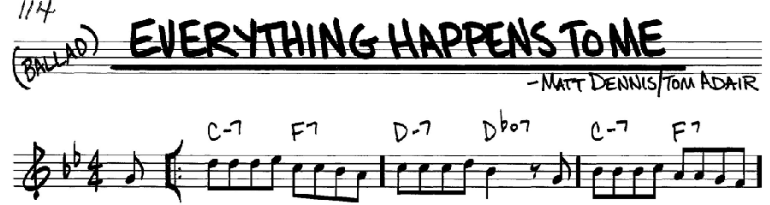
\includegraphics[width=0.5\linewidth]{everything}}. In order to formally solve this problem we need the following proposition.
\begin{proposition}
	Let $K$ be a $\Sigma$-finite kernel (the most general property we can think of) from $(E,\E)$ into $(F,\F)$. We consider measurable functions with respect to the product space: for every positive funtion $f\in\E\otimes\F$ we have that:
	\[Tf(x)=\int_FK(x,\dy)f(x,y)\qquad x\in E\]
	And this object defines a function $Tf\in\E_+$. This is a similar operation to the previous theorem. Moreover the transformation $T:(\E\otimes\F)_+\mapsto \E_+$ is linear and continuous under increasing limits, that is:
	\begin{enumerate}[a)]
		\item if we take $f,g\in(\E\otimes\F)_+$ and $a,b\in\R_+$ we have
		\[T(af+bf)=aTf+bTg;\]
		\item $Tf_n\nearrow Tf$ for $\every$ sequence $(f_n)_{_{n}}\subset(\E\otimes\F)_+$ with $f_n\nearrow f$.
	\end{enumerate}
\end{proposition}
So, similarly to the previous theorem we have constructed this operator $Tf$ which operates on the function set $(\E\otimes\F)_+$ giving us a positive $\E$-measurable function. So we can start from this function to build a method to construct measures on the product space $(\E\otimes\F)_+$ with its related \sa{}.
\begin{theorem}
	\emph{Extension of measures on product spaces}.\\
	Let $\mu$ be a measure on the measurable space $(E,\E)$. Let $K$ be a $\Sigma$-finite\footnote{Erm... what the sigma?} transition kernel from space $(E,\E)$ into $(F,\F)$. Then:
	\begin{enumerate}[\circnum]
		\item if we take our function $f(x,y)$, integrate it against our kernel $K(x,\dx)$ over $F$ and then integrate again against measure $\mu$ over $E$, the operation 
		\[\pi f=\int_E\mu(\dx)\int_FK(x,\dy)f(x,y)\]
		defines a measure $\pi$ on $(E\times F,\E\otimes\F)$;
		\item if $\mu$ is $\sigma$-finite and $K$ is $\sigma$-bounded then $\pi$ is $\sigma$-finite and it is the unique measure on $(E\times F,\E\otimes\F)$ satisfying
		\[\pi(A\times B)=\int_A\mu(\dx)K(x,B)\qquad\every A\in\E,B,\in\F.\]
	\end{enumerate}
\end{theorem}
So by means of kernels we are able to define measures on product spaces in this way\footnote{I crave to be released from this prison of flesh.}.
\begin{remark}
	When the kernel that we used to extend the measure has the form 
	\[K(x,B)=\nu(B)\]
	for some $\Sigma$-finite measure $\nu$ on $(F,\F)$, which means that it only depends on $B$ and is therefore a measure, then we obtain the \emph{product measure}
	\[\pi=\mu\nu.\]
\end{remark}
But what should we do when we have more than 2 spaces\footnote{I have an idea.}? On finite product spaces we introduce in the same manner the product measure 
\[\pi=\mu_1\mu_2\cdots\mu_n\]
where $\mu_i$ is $\Sigma$-finite on $(E_i,\E_i)$ for $\every i=1,\ldots,n$.
So we can induce the presence of another measure from the product measure using the kernels, without assuming independence in the construction.
\begin{example}
	Here we tackle $n=3$. Take $\mu_1$ on $(E_1,\E_1)$, the transition kernel $K_2$ from $(E_1,\E_1)$ into $(E_2,\E_2)$ and the transition kernel $K_3$ from $(E_1\times E_2,\E_1\otimes\E_2)$ into $(E_3,\E_3)$. Not how we only defined the first measure and then only the transition kernels. We will use these fucking kernels to "move" from measure to measure and from space to space. We have
	\[\pi f=\int_{E_1}\mu(\dx_1)\int_{E_2}K_2(x,\dx_2)\int_{E_3}K\Big((x_1,x_2),\dx_3\Big)f(x_1,x_2,x_3)\]
	with $f$ positive and $(\E_1\otimes\E_2\otimes\E_3)$-measurable. So we defined a measure $\pi$ which is different from the product measure we recalled earlier (actually that product measure is a special case of this measure) and $\pi$ is a measure on the 3-dimensional product space. Writing $\pi$ in differential form:
	\begin{align*}
		\pi(\dx_1,\dx_2,\dx_3)&=\mu(\dx_1)K_2(x,\dx_2)K\Big((x_1,x_2),\dx_3\Big)\\
		&=\mu_1K_2K_3.
	\end{align*}
\end{example}
This is for finite product spaces but we can also extend this to infinte product spaces\footnote{Why. Stop.}.\\
What should we expect now?
\section{Expectation}
Well that was a cheap joke. We already know the meaning of expectation from our undergraduate courses... but here we will rock our world and learn some new interpretations. Let's start with measure theory\footnote{We have a great time ahead, I see.}. In probability the concept of expectation is strictly tied with the concept of integral: we could say they are almost the same thing.
\begin{definition}
	Let $X$ be a real valued $(\overline{\R})$ \rv{} on the probability space $(\Omega,\mathscr{H},\pr)$. The \emph{expectation} or \emph{expected value} of $X$ is
	\[\ev X=\int_\Omega X(\omega)\pr(\dw).\]
\end{definition}
	\begin{notation}
		\[\ev X=\int_\Omega X(\omega)\pr(\dw)=\int_\Omega x\dif\pr.\]
		There is always the compact notation we use for integrals
		\[\pr X.\]
	\end{notation}
We are integrating the function over the space where it is defined, but since we are using Lebesgue integration we need to integrate with respect to a measure... which is the probability measure $\pr(\dw)$. This is a little bit different from the classic definition, but this is more correct.
\begin{remark}
	The expectation of $X$ exists \underline{if and only of} the related integral exists. So the existence of the expectation is the existence of the integral.\\
\end{remark}
\begin{wrapfigure}{R}{0.6\textwidth}
	\centering
	
\includegraphics[width=0.6\textwidth]{kept3}
	\caption{And then he turned himself into a pickle, funniest shit I've ever seen.}
	\label{fig:kept3}
\end{wrapfigure}
Consider the \rv{} $X$, with its positive part $X^+$ and its negative part $X^-$. Moreover, remember that 
\[X=X^+-X^-\]
where both the positive part \textit{and} the negative part are positive functions (remember?\footnote{No. Happy?}). If we apply the expectation to $X$, by the linearity of the integral operator we have that:
\[\ev X=\ev X^+-\ev X^-.\]
Where, in particular:
\[\ev X^+=\int_\Omega X^+\pr(\dw)=\begin{cases}
	<+\infty\\
	+\infty
\end{cases}\]
and
\[\ev X^-=\int_\Omega X^-\pr(\dw)=\begin{cases}
	<+\infty\\
	+\infty
\end{cases}\]
The problem arises when both the expectation of the positive part and the expectation of the negative part are simultaneously infinite.\\
Further, we say that $\ev X$ exists finit e when at the same time both expectations are finite: 
\[\ev X^+<+\infty,\quad X^-<+\infty.\]
In this case
\[\ev X=\ev X^+-\ev X^-<\infty.\]
Finally, remember from undergraduate courses:
\[\ev X^+\ev X^-=\ev |X|\]

So if we check that the expectation of the absolute value is finite this will imply that the expectation of $X$ is finite in both the negative and the positive part. A \rv{} with finite expectations is said to be \emph{integrable}.
\begin{remark}\label{eh}
	This is connected to the definition of expectation of a \rv{} that we already know. Consider the "change of variable" formula for Lebesgue integrals (see \cinlar, formula 5.3 page 30): consider $f\in\E$ and $h:(F,\F)\mapsto(E,\E)$. We integrate
	\[\int_F\nu(\dx)f\Big(h(x)\Big)=\int_E\mu(\dy)f(y)\]
	where $\mu$ is a measure on $(E,\E)$ and is the \textit{image measure} of $\nu$ through the function $h$. For us:
	\begin{itemize}
		\item $h\equiv X$;
		\item $(F,\F)\equiv(\Omega,\mathscr{H})$;
		\item $\nu=\pr$;
		\item $\mu$ is the distribution of $X$;
		\item $(E,\E)\equiv(\R,\B_{\R})$.
	\end{itemize}
	So the formula becomes
	\[\int_\Omega\pr(\dw)f\Big(X(\omega)\Big)=\int_{\R}\mu(\dx)f(x)\]
	with $f$ Borel-measurable. Now the last step is to choose a specific function $f$, for which we choose the \textit{identity function} so that
	\[\int_\Omega\pr(\dw)X(\omega)=\int_{\R}\mu(\dx)x.\]
	Here's the formula that we used to calculate the expectation in the undergraduate years! To be honest, that's what you'll ever really use in the sad case of you working in this field. If the distribution is absolutely continuous with respect to the lebesgue measure we get
	\[\int_{\R}\mu(\dx)x=\int_{\R}f_X(x)\dx\cdot x\]
	otherwise, if it is absolutely continuous with respect to a counting measure we get
	\[\int_{\R}\mu(\dx)x=\sum_{i=1}^{\infty}\pr(X=x_i)\cdot x_i.\]
	\begin{notation}
		Forget riemann integrals and sums, fucker, from now on you must learn to use 
		\[\int_{\R}\mu(\dx)x.\]
	\end{notation}
\end{remark}
\subsection{Properties of expectation}
\begin{itemize}
	\item \emph{Positivity}:
	\[X\geq0\implies\ev X\geq0.\]
	Remember that we are talking about \rv s, so when we say $X\geq 0$ we actually mean ``$X\geq 0$ almost surely with respect to $\pr$''\footnote{Because reality crumbles in front of the chaotic horror of randomness. A similar fate is reserved to my balls.}.
	\item \emph{Monotonicity}:
	\[X\geq Y\geq0\implies\ev X\geq\ev Y.\]
	\item \emph{Linearity}:
	\[X,Y\geq0\implies\ev(aX+bY)=a\ev X+b\ev Y.\]
	\item \emph{Insensitivity}:
	\[X,Y\geq0,\; X=Y\text{ almost surely }\implies\ev X=\ev Y.\]
	\item \emph{Monotone convergence}: if we have, for $X_n\geq-0$,
	\[(X_{n})_{_{n}}\nearrow X\implies\ev X_n\nearrow \ev X.\]
	\item \emph{Fatou's Lemma}: for $X_n\geq0$ we have
	\[(X_{n})_{_{n}}\geq0\implies\ev\liminf X_n\leq\liminf\ev X_n.\]
	\item \emph{Dominated convergence}: if $(X_{n})_{_{n}}$ is a sequence of \rv s such that $\every n |X_n|\leq Y$ and $Y$ has finite expectation (it is integrable) and $\lim_{n\to\infty}X_n$ exists, then 
	\[\ev\lim_{n}X_n=\lim_{n}\ev X_n.\]
	\item \emph{Bounded convergence}: if we have a sequence of \rv s $(X_n)_{_{n}}$ such that $|X_n|\leq b<\infty$ and $\lim_{n\to\infty}X_n$ exists, then
	\[\ev\lim_{n}X_n=\lim_{n}\ev X_n.\]
\end{itemize}
\begin{remark}
	$X$ is positive (or non negative) and $\ev X=0$ \underline{if and only if} $X=0$ almost surely. 
\end{remark}
\begin{remark}
	If we restrict $\ev X$ and $\ev Y$ on the subset $H$ we get:
	\[\text{if }\ev X\indi_H\geq\ev Y\indi_H\quad\every H\implies X\geq Y\text{ a.s.}\]
\end{remark}
\begin{theorem}\label{expprob}
	Let $X$ be a \rv{} taking values in $(E,\E)$ and be measurable relative to $\mathscr{H}$ and $\E$. If $\mu$ is the distribution of $X$ then
	\begin{equation}
		\ev f\circ X=\mu f,\qquad\every f\in\E_+ \tag{$\star$} \label{diocane}
	\end{equation}
	Conversely, if \ref{diocane} holds for some measure $\mu$ on $(E,\E)$ and $\every f\in\E_+$, then $\mu$ is the distribution of $X$.
\end{theorem}
\begin{fancyproof}
	The proof should be simple. The first statement is basically the \hyperref[eh]{change of variable} formula, rephrasing the theorem on integration with respect to image measures.
	The second converse statement requires more thought. If \ref{diocane} holds $\every f\in\E_+$, then it holds also for $f=\indi_A$ for $A\in\E$ and we have that if we want to calculate the measure 
	\[\mu(A)=\mu\indi_A=\ev\indi_A\circ X=\pr(X\in A).\]
	So we have identified this measure with the distribution of the random variable and hence $\mu$ is the distribution of $X$.
\end{fancyproof}
\begin{example}
	\begin{enumerate}[\circnum]
		\item The \emph{variance} of the \rv{} $X$ is
		\[\var X=\ev(X-\ev X)^2.\]
		\item Consider the expectation of an exponential transform of $X$:
		\[\tilde{\mu}_r=\ev e^{-rX}=\int_{\R_+}e^{-rx}\mu(\dx),\qquad r\in\R_+,x>0.\]
		This is known as the \emph{Lapalce transform} of distribution $\mu$. It is connected to the moment generating function of a distribution.
		\item We could be interested in the expectation of another exponential transform:
		\[\hat{\mu}_r=\ev e^{irX}=\int_{\R}\mu(\dx)e^{irx}\]
		and, exploiting the representation of complex numbers,
		\[\hat{\mu}_r=\int_{\R}\mu(\dx)\cos(rx)+i\int_{\R}\mu(\dx)\sin(rx)\]
		and this is called the \emph{characteristic function} of $\mu$.
		\item Consider $X$, a \rv{} taking values in $\overline{\N}$. Consider
		\[\ev z^X=\sum_{n=1}^{\infty}z^n\cdot\pr(X=n),\qquad z\in[0,1].\]
		This is called \emph{probability generating function of $X$}.
	\end{enumerate}
	These are all special kinds of expectations.
\end{example}
\begin{remark}
	The expectation $\ev X$ is in some sense ``optimal'': what the fuck? It is ``optimal'' because it is our best estimate of $X$. Imagine we are given the following integral:
	\[f(a)=\int_\Omega \Big(X(\omega-a)\Big)^2\pr(\dw).\]
	Let us now derive the minimum value for the number $a$, that is the best value that cancels out the random variable $X$. Just take the derivative with respect to $a$:
	\begin{align*}
		\frac{\dif}{\dif a}f(a)&=\int_\Omega\pr(\dw)\Bigg(-2\Big(X(\omega)-a\Big)\Bigg)=0\\
		&=2a\int_\Omega\pr(\dw)-2\int_\Omega\pr(\dw)X(\omega)=0\\
		&\implies a= \underbracket[0.6pt]{\int_\Omega\pr(\dw)X(\omega).}_{\mathclap{\text{definition of }\ev X}}
	\end{align*}
\end{remark}
We must now recall some famous inequalities.
\begin{itemize}
	\item \emph{Markov inequality}: this is for positive, real-valued random variables. Let $X$ be a positive and real-valued \rv. We may be interested in the probability that $X$ exceeds some positive value $b$. We know that
	\[\pr(X>b)\leq\frac{1}{b}\ev X\qquad\every b>0.\]
	\item \emph{Chebyshev inequality}: this is too for positive, real-valued random variables. Let $X$ be a positive and real-valued \rv. What we have is that
	\[\pr\Big(|X-\ev X|>\varepsilon\Big)\leq\frac{\var X}{\varepsilon^2},\qquad\varepsilon>0.\]
	\item \emph{Jensen inequality}: Let $X$ be a real-valued \rv{} with finite expectation (integrable) and let $f$ be a convex function on $\R$. Then
	\[\ev f(X)\geq f(\ev X).\]
	If the function is concave the inequality is the opposite.
\end{itemize}
\begin{definition}
	Let $X,Y$ be two real-valued \rv s with finite variance. The \emph{covariance} between $X$ and $Y$ is
	\[\cov(X,Y)=\ev (X-\ev X)(Y-\ev Y).\]
\end{definition}
If $X$ and $Y$ are independent, then $\cov(X,Y)=0$ (try to prove it but it is easy even for me\footnote{Proceeds \textit{not} to do it.}).
\begin{remark}
	If we want to calculate the variance of two real-valued \rv s then
	\[\var(X+Y)=\var(X)+\var(Y)+2\cov(X,Y).\]
	This can be proven very easily. Of course, if $X$ and $Y$ are an independency then $\cov(X,Y)=0$ and $\var(X+Y)=\var(X)+\var(Y)$.
\end{remark}
Consider $\ev |X|<+\infty.$ We think of \rv s with finite expectation in absolute value as ``well-behaved'', without any crazy jumps or fluctuations. So it could be interesting to look for a way to treat all of these \rv s with finite expectation in the same way.
\begin{remark}
	A \rv{} (real-valued) random variable with finite expectations is called \emph{integrable \rv}.
\end{remark}
We are going back to functional analysis now. Brace yourselves.
\subsection{$L^p$ spaces}
We start, as usual, with the $(\Omega,\mathscr{H},\pr)$ probability space, with the real-valued \rv{} $X$ and the parameter $p\in[1,\infty]$. Why doesn't $p$ start from 0? It's dumbass mathematical reason we won't and shouldn't care about\footnote{$L$ in $L^p$ stands for Lebesgue space. If $p<0$ these spaces do not have the property of Lebesgue spaces so we don't care.}.\\
Define the so-called $L^p$-norm of $X$ as:
\[\norm{X}_p=\left(\ev|X|^p\right)^{\frac{1}{p}},\qquad p<+\infty.\]
Remember that expectations are integrals. We can also define a \textit{sup-norm}:
\[\norm{X}_{\infty}=\inf(b\in\R_+:|X|\leq b\text{ a.s.}).\]
So, taking a \rv{} $X$ and fixing $p$ we can calculate a number to attach to this \rv{}.
\begin{example}
	Take $p=1$. Our $L^p$-norm would then be
	\[\norm{X}_1=\ev|X|.\]
\end{example}
No shit. But as long as $p$ is finite we can technically write the $L^p$ norm of the \rv. The same goes for $p=\infty$, but with the different definition. We will call the \textit{sup-norm} \emph{essential supremum of $X$}. This name has a meaning: imagine the random variable $X$ ``folded'' by the absolute variable. We are interested in the number $b$ for which the probability mass is more or left all to the left of this number.
\begin{notation}
	\[ \mathrm{essup}(X)= \norm{X}_{\infty}.\]
\end{notation}
\begin{remark}
	If $\norm{X}_p=0\implies X=0$ almost surely. Remember that the $L^p$-norm has an absolute value, so if the norm is 0 then the \rv{} must be 0 everywhere. 
\end{remark}
If we fix a number $c\geq0$ we have
\[\norm{cX}_p=c\norm{X}_p.\]
If we have $1\leq p\leq q\leq+\infty$ then
\[0\leq\norm{X}_p\leq\norm{X}_q\leq+\infty.\]
\begin{definition}
	The collection of real-valued \rv{}s $X$ with $\norm{X}_p<+\infty,\;p\in[1,\infty]$ is called \emph{$\mathbf{L^p}$}.
\end{definition}
So we are creating sub-collections of real-valued \rv s such that they have a finite norm. The space $L^p$ is a subset of the space of all \rv s.
\begin{remark}
	X is in $L^{p},\;p \in [1,\infty\color{red}\boldsymbol{)}$ if and only if $|X|^{p}$ is integrable and $X$ is in $L^{\infty}$ if and only if $X$ is almost surely bounded.
\end{remark}
\begin{remark}
	If $1\leq p\leq q\leq+\infty$ then
	\[L^{q}\subset L^{p}\]
\end{remark}
So the $L^p$ spaces are one inside the other, with $L^{\infty}$ being the smallest of them all and $L^{1}$ being the biggest. Think about the meaning: $L^{1}$ is the space of all integrable \rv s; $L^{2}$ is the space for which $|X|^{2}$ is integrable, but if $|X|^{2}$ is integrable so is $|X|$... and so on. We can thus prove certain properties for the whole class and this will extend to smaller classes.\\
The regularity of these functions is evident when we look at $L^{\infty}$: the functions that belong in this space are very regular because they are almost surely bounded and therefore their support doesn't explode towards infinity\footnote{Professor Polito said: ``Good guys''. :3}.
\begin{remark}
		Some useful inequalities...
\begin{itemize}
	\item\emph{Minkowsky inequality}: 
	\[\norm{X+Y}_{r}\leq\norm{X}_p-\norm{Y}_{p}.\]
	\item \emph{Hölder inequality}:
	\[\norm{XY}_{r}\leq\norm{X}_p\norm{Y}_q\]
	where $\frac{1}{p}+\frac{1}{q}=\frac{1}{r}$ for $p,q,r\in[1,\infty)$.
	\item \emph{Jensen inequality}:
	Consider:
	\begin{itemize}
		\item a convex domain $D$ in $\R^d$;
		\item a continuous and concave function $f:D\mapsto\R$;
		\item a sequence of \rv s $X_1,X_2,\ldots,X_d$ integrable (in $L^{1}$ space) for which $(X_1,X_2,\ldots,X_d)\in D$ almost surely.
	\end{itemize}	
	Then
	\[\ev f(X_1,X_2,\ldots,X_d)\leq f\Big(\ev (X_1,X_2,\ldots,X_d)\Big).\]
\end{itemize}
\end{remark}
When we talk about integrability, we have this useful lemma:
\begin{lemma}
	Let $X$ be a real-valued \rv{}. $X$ is integrable if and only if
	\[\lim_{b\to\infty}\ev|X|\indi_{(|X|>b)}=0.\]
\end{lemma}
This lemma states that this is an equivalent condition for integrability. The random variable $|X|\indi_{(|X|>b)}=0$ is equal to 0 until $b$ and equal to the absolute value of $X$ after $b$. So we are effectively truncating the random variable but maintaining the right tail. 
This means that if we integrate only the tails of the \rv{} we wouldn't get much information (we can say that the tail is \textit{thin}).
\begin{fancyproof}
	Let's call $Z_b$ the truncated random variable $|X|\indi_{(|X|>b)}=0$. Note that $Z_b\leq|X|$ and that $Z_b\xrightarrow[b\to\infty]{}0$. Since $X$ is integrable, we use the dominated convergence theorem:
	\[\lim_{b\to\infty}\ev|X|\indi_{(|X|>b)}=\ev\Big[\lim_{b\to\infty}\indi_{(|X|>b)}\Big]=0.\]
	The first statement is proved. Conversely, if $\ev Z_b\to0$, we can choose $b$ large enough such that
	\[\ev Z_b\leq 1.\]
	Then 
	\[|X|\leq b+Z_b.\]
	This is not immediate but it's true. Due to linearity of expectation, we know that
	\[\ev|X|\leq b+\ev Z_b\]
	but we know that $\ev Z_b\leq 1$ so
	\[\ev|X|\leq b+1\leq\infty.\]
\end{fancyproof}
\subsection{Uniform integrability}
\begin{definition}
	A collection of random variables K is said to be \emph{uniformly integrable} if
	\[k(b)=\sup_{X\in K}\left(\ev|X|\indi_{(|X|>b)}\right)\]
	goes to 0 as $b\to\infty$. 
\end{definition}
Note that it is a function of $b$. We consider the supremum of the collection to be ``conservative'': if the supremum goes to 0 then I know the whole collection will.
\begin{remark}
	\begin{enumerate}[\circnum]
		\item If $K$ is finite and each $X\in K$ is integrable then $K$ is uniformly integrable.
		\item If $K$ is dominated by an integrable \rv{} $Z$ then it is uniformly integrable.
		\item Uniform integrability of a collection $K$ implies the so-called $L^{1}$-boundedness, which means
		\[k\subset L^{1}\quad\text{and}\quad k(0)=\sup_{K}\ev |X|<\infty.\]
		Note that $k(0)$ considers the whole \rv{} without truncation.
		\begin{fancyproof}
			\[\ev|x|\leq b+k(b)\qquad \every X\in K.\]
			So, since now every \rv{} is in $K$ and $K$ is uniformly integrable, we use this property of $K$ to choose a value for $b$ such that $k(b)\leq 1$ and therefore it is finite.
		\end{fancyproof}
		\item We know that uniform integrability implies $L^{1}$... but the converse is not true. We can prove it by a counterexample.
		\begin{fancyproof}
			Consider the probability space $$\Big((0,1),\B_{(0,1)},\underbrace{\leb}_{\mathclap{\text{Lebesgue measure}}}\Big).$$ Normally the Lebesgue measure is infinite on the whole support, but if we restrict the measure on the unit interval then the lebesgue measure has maximum value 1 and so it is a probability measure.\\
			Consider the collection
			\[K=(X_n)_{_{n\geq1}}\qquad\mathrm{s.t.}\;X_n=\begin{cases}
				n, &\omega\leq\frac{1}{n}\\
				0,  &\mathrm{otherwise}
			\end{cases}\]
			Note that \[
			\every n\quad\ev X_n=1
			\]
			That is, $K$ is $L^{1}$-bounded.\\
			But if we calculate $k(b)$ we realize it is equal too 1 for each $b$, so
			\[\ev X_n\indi_{(X_n>b)}=\ev X_n=1\qquad\every n>b\]
			Therefore the collection $K$ is \textit{not} uniformly integral.
		\end{fancyproof}
		\item If $K$ is $L^{p}$-bounded with $p>1$ then it is uniformly integrable with $f(x)=x^p$. \\
		To prove this we recur to the following proposition:
		\begin{proposition}
			Suppose it exists a positive borel function $f$ on $\R_+$ such that
			\[\lim_{x\to\infty}\frac{f(x)}{x}=\infty\]
			and write 
			\begin{equation}
				c=\sup_{X\in K}\ev f\circ|X|. \tag{$\star$} \label{desiderolamorte}
			\end{equation}
			If $c\leq \infty$ then $K$ is uniformly integrable.
		\end{proposition}
		\begin{fancyproof}
			We are talking about the absolute value of $X$, so we don't lose generality if we talk about positive \rv{}s. Let us assume, then, that $X\in\R_+$. Let us replace $f$ with $f\vee1$ if necessary and assume $f\geq1$.\\
			Let $g(x)=\frac{x}{f)=(x)}$ and note that if we are looking at the tail of the \rv{} we get
			\[X\indi_{(X_n>b)}=(f\circ X)(g\circ X)\indi_{(X_n>b)}.\]
			This is true because $(f\circ X)(g\circ X)=\cancel{f(x)}\frac{x}{\cancel{f(x)}}$.\\
			Let us now bound this quantity:
			\begin{align*}
				X\indi_{(X_n>b)}&=(f\circ X)(g\circ X)\indi_{(X_n>b)}\\
				&\leq (f\circ X) \sup_{x>b}g(x).
			\end{align*}
			If now $X\in\R$ (not necessarily positive) we can write this inequality as
			\begin{equation*}
				|X|\indi_{(|X|>b)}\leq (f\circ|X|) \sup_{x>b} g(x).
			\end{equation*}
			Take the expectation and the $\sup_{K}$, using equation \ref{desiderolamorte} (remember that $k(b)=\sup_{X\in K}(\ev|X|\indi_{(|X|>b)})$):
			\[k(b)\leq c\cdot \sup_{x>b}g(x).\]
			To study the behaviour in the limit for $b\to\infty$, we must study separately $c$ (that is a finite number) and $\sup_{x>b}g(x)$ (that for $b\to\infty$, and therefore for $x\to\infty$, goes to 0 as $g(x)=\frac{x}{f(x)}=\frac{1}{\frac{f(x)}{x}\to\infty}$).
			Hence, $K$ is uniformly integrable.
		\end{fancyproof}
	\end{enumerate}
\end{remark}
Let's see one more\footnote{There will be consequences.} theorem about uniform integrability.
\begin{theorem}
	The following are equivalent:
	\begin{enumerate}[\circnum]
		\item $K$ is uniformly integrable;
		\item $h(b)=\sup_{K}\int_{b}^{+\infty}\dy \pr(|X|>y)\xrightarrow[b\to\infty]{}0$;
		\item $\sup_{K}\ev f\circ |X|<+\infty$ for some increasing convex function $f$ on $\R_+$ such that
		\[\lim_{x\to\infty}\frac{f(x)}{x}=+\infty.\]
	\end{enumerate}
\end{theorem}
So we can consider all of these as alternative definition of uniform integrability and this is important because it is the extension of the concept of integrability for \rv s. For example, we will treat only uniformly integrable martingales, which are good boys who's mommy good boy you are.
\section{\sa s and \rv s}
There is a way to connect \sa s and \rv s and we will see how linked the two objects are. Consider a \rv{} $X$ taking values in $(E,\E)$. Then consider the collection of all inverse image of the set $A$ through the \rv{} $X$:
\[\sigma X=X^{-1}\E=\left\{X^{-1}A:A\in\E\right\}\]
\begin{figure}[H]
	\centering
	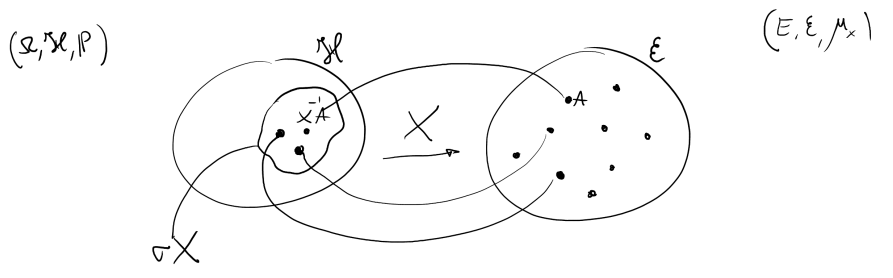
\includegraphics[width=0.9\linewidth]{screenshot005}
	\caption[Professor Polito draws circles and arrows]{Remember that $\mathscr{H}$ is made of the subsets of $\Omega$ and that $\E$ is made of the subsets of $E$. Also, $\sigma X$ is a subset of $\mathscr{H}$.}
	\label{fig:screenshot005}
\end{figure}
\begin{wrapfigure}[12]{L}{0.28\textwidth}
	\centering
	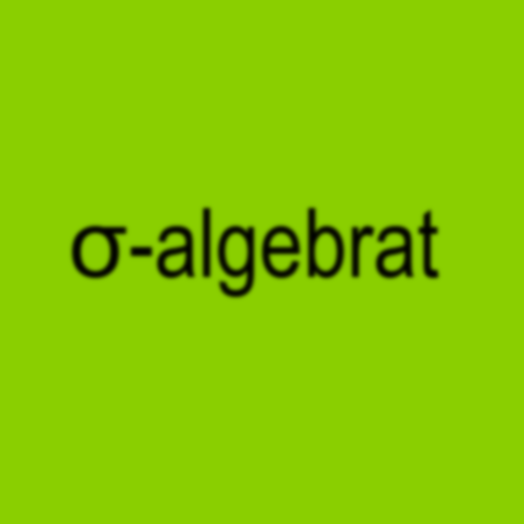
\includegraphics[width=0.28\textwidth]{brat}
	\caption[I'm so Julia]{I'm just a gurl\protect\footnotemark.}
	\label{fig:brat}
\end{wrapfigure}
We call it $\sigma X$ because it is the \emph{\sa{} generated by $X$}. It is basically the set of all inverse images of $X$ that sit in $\E$. 
This object is simple... 
Every time we introduce a \rv{} we have a connection to two spaces: there is the probability space (for instance $(\Omega,\mathscr{H},\pr)$), the arrival space $(E,\E)$ and the \sa{} $\sigma X$. 
By means of the measurability of $X$ (remember the \hyperref[measur]{definition of measurability}?) we are simultaneously constructing all the inverse images of the element of the \sa{} $\E$ in the arrival space. 
If I consider all of them together we can prove that the resulting set is actually a \sa{} (the one generated by $X$) and it is a subset of $\mathscr{H}$, as we see in figure \ref{fig:screenshot005}. This is very important, for reasons that elude me.\par
\footnotetext{This image will mean absolutely nothing to you unless you were terminally online in the summer of 2024. Otherwise it is hilarious.}
\begin{remark}
	$\sigma X$ is the smallest \sa{} $\G$ on $\Omega$ such that $X$ is measurable relative to $\G$ and $\E$.
\end{remark}
Take now $T$ as an arbitrary index set (which can be countable or uncountable). Consider $\every t\in T,\;X_t$ being a \rv{} taking values in the measurable space $(E_t,\E_t)$. Then
\[
\sigma\left\{X_t:t\in T\right\}=\sigma(X_t)_{_{t\in T}}=\sigma\left(\bigcup_{t\in T}\sigma X_t\right).
\]
This is just the union of the \sa s generated by the by the \rv{} $X$: we consider the \sa{} of this union just to make sure that this union is, indeed, a \sa{}.\par
\begin{notation}
	Remember that the \sa{} generated by the collection $(X_t)_{_{t\in T}}$ is noted as
		\[\bigvee_{t\in T}\sigma X_t=\sigma\left(\bigcup_{t\in T}\sigma X_t\right)\]
\end{notation}
Furthermore, it is the smallest \sa{} $\G$ on $\Omega$ such that $\every t\in T$ the \rv{} $X_t$ is measurable relative to $\G$ and the corresponding $\E_t$.
\begin{remark}
	Consider the collection $X={(X_{t})}_{t\in T}$ to be the \rv{} taking values in the product space 
	\[\bigotimes_{t\in T}(E_t,\E_t).\]
	Define now $X(\omega)$ to be the point $\Big(X_t(\omega)\Big)_{t\in T}$. The mapping 
	\[\omega\mapsto X_t(\omega)\]
	is a \rv{} and is called \emph{$t$-coordinate of $X$}.
\end{remark}
\begin{proposition}
	If $X=(X_{t})_{_{t\in T}}$ then $$\sigma X=\sigma{\Big(X_{t}\Big)}_{t\in T}$$
\end{proposition}
So if we generate the \sa{} from the collection as $\bigvee_{t\in T}\sigma X_t$ and we generate the \sa{} from a collection seen a single random variable (as $\sigma X=X^{-1}\E$) we end up with the same object. Professor Polito think this is a nice thing. I am very keen on that man, to be honest. His enthusiasm is almost contagious.\par
Remember: when we define a \rv{} we actually do two things:
\begin{itemize}
	\item we induce a distribution (that is a probability measure) to the arrival space:
	\[(\Omega,\mathscr{H},\pr)\xrightarrow[X]{}(E,\E,\mu_x);\]
	\item we induce the existence of a special \sa{} that links the \sa{} $\mathscr{H}$ and the sa $\E$ (that is the \sa{} $\sigma X$).
\end{itemize}
We can define a new \rv{} $V$ which is measurable with respect to the \sa{} $\sigma X$. Since we defined $V$ as a \rv{} then it is automatically measurable with respect to $\HS$ and $\E$, but in particular when $V$ is also measurable with respect to $\sigma X$ then it has a special representation. Before going through the theorem, let's revise once more a couple of measure theory concepts:
\begin{revise}
	\begin{definition}
		The collection of functions $\mathcal{M}$ is called \emph{monotone class} if:
		\begin{enumerate}[a)]
			\item $\indi\in\mathcal{M}$;
			\item let $f,g\in\mathcal{M}_b$ (bounded functions in $\mathcal{M}$) and let $a,b\in\R$. Then $af+bg\in\mathcal{M}$;
			\item $(f_n)\subset\mathcal{M}_+$ with $f_n\nearrow f$. Then $f\in\mathcal{M}$.
		\end{enumerate}
	\end{definition}
	\begin{theorem}
		\emph{Monotone class theorem for functions}.
		Let $\mathcal{M}$ be a monotone class of functions on $E$. Suppose that $\indi_A\in\mathcal{M}$ for each $A\in\mathcal{C}$ where $\mathcal{C}$ is some $\pi$-system generating $\E$.\\
		Then, $\mathcal{M}$ includes all positive $\E$-measurable functions and all bounded $\E$-measurable functions.
	\end{theorem}
\end{revise}
	We are going to use this theorem in the proof of the following theorem..
	\begin{theorem}\label{teodelta}
		\emph{``Theorem $\Delta$''}:\\
		Let $X$ be \rv{} taking values in the measurable space $(E,\E)$. A mapping
		\[V:\Omega\mapsto\overline{\R}\]
		belongs to $\sigma X$ \underline{if and only if}
		\[V=f\circ X\]
		for some deterministic function $f\in\E$.
	\end{theorem}
The proof will be long as fuck.
\begin{fancyproof}
	(Sufficiency)\\
	Consider a collection $\mathcal{M}$ of all $V$ of the form 
	\[V=f\circ X,\qquad f\in\E.\]
	We would like to prove that $\mathcal{M}\subset\sigma X$, that is to say: if we have a function in the form of $V$ the it is $\sigma X$-measurable. Measurable functions of measurable functions are still measurable: $f$ is $\E$-measurable and $X$ is a \rv: therefore $X$ is $\HS$-measurable but $X$ is also measurable with respect to the \sa{} generated by itself.\\
	Hence
	
	\[V\text{ is }\sigma X\text{-measurable.}\vspace{1cm}\]
	(Necessity)\\
	We are planning to show that $\mathcal{M}\supset \sigma X$. 
	\begin{enumerate}
		\item We show that $\mathcal{M}$ is a monotone class of functions: we must check the three properties of the class;
		\begin{enumerate}
			\item $\indi_E\in\mathcal{M}$ because $\indi_E=f\circ X$ with $f(x)=1\;\every x\in E$.
			\item let $U,V\in\mathcal{M}_b$. Let $a,b\in\R$. Plainly
			\[U=f\circ X,\qquad V=g\circ X\]
			for the right choice of $f,g\in\E$. Consider now the combination
			\[aU+bV=h\circ X\]
			with $h=af+bg$. Note that $h\in\E$. Hence
			\[aU+bV\in\mathcal{M}.\] H
			\item consider $(V_n)\subset\mathcal{M}_+$ and $V_n\nearrow V$. For each $n$, $\exists\,f_n\in\E$ such that $V_n=f_n\circ X$. We now want to check that $V\in\mathcal{M}$.\\
			Consider 
			\[f=\sup_{n} f_n\in\E\]
			and
			\[V=\sup_{n}V_n=\sup_{n} f_{n}(X)=f(X)\]
			Hence $V\in\mathcal{M}$.
		\end{enumerate}
		\item Consider $H\in\Omega$ such that it is in $\sigma X$. If it is in $\sigma X$ then this means that $H$ comes from the inverse image of a set $A$ in $\E$:
		\[H=X^{-1}A\]
		for some $A\in\E$. So
		\[\indi_H=\indi_A\circ X\in\mathcal{M}.\]
		So the class $\mathcal{M}$ contains all the indicators of the events that are contained in $\sigma X$. We need to check, for the monotone class theorem, what happens to the indicators of the elements of the $\pi$-system which in this case would be $\sigma X$... that is a \sa{} but being a \sa{} means also being a $\pi$-system.\\
		We have proven that $\mathcal{M}$ contains all the indicators in $\sigma X$ and applying the monotone class theorem for functions we have that 
		$\mathcal{M}$ contains all positive \rv s that are $\sigma X$-measurable.
		\item Let $V\in\sigma X$ be arbitrary. Then of course $V^{+}\in\sigma X$ and it is positive (the same can be said for $v^{-}$). Hence $V^{+}=g\circ X$ for some $g\in\E$ and $V^{-}=h\circ X$ for some $h\in\E$. Then 
		\[V=V^{+}-V_{-}=f\circ X\]
		where
		\[f(x)=\begin{cases}
			g(x)-h(x), &\text{if }g(x)\wedge h(x)=0\\
			0, &\text{otherwise}
		\end{cases}\]
		and $f\in\E$.
 	\end{enumerate}
 	This concludes $\sigma X\subset\mathcal{M}$.
\end{fancyproof}
\begin{corollary}
	For each $n\in\N^*$, let $X_n$ be a \rv{} taking values in $(E_n,\E_n)$. A mapping
	\[V:\Omega\mapsto\overline{\R}\]
	is $\sigma (X_n)_{n\in\N^*}$-measurable if and only if
	\[V=f(X_1,X_2,X_3,\ldots)\]
	For some deterministic functtion $f\in\bigotimes_n\E_n$.
\end{corollary}
Remember that $N^*$ are the natural numbers without 0.
\begin{remark}
	The above corollary can also be extended to uncountable collections. Should it? I don't know. You tell me.
\end{remark}
Why did we destroyed our balls with this section about \sa s?
\subsection{Filtrations}
Let $T$ be a subset of $\R$. Let $\F_t$ be a sub-\sa{} of $\HS\;\every t\in T$. The family $\F=(\F_t)_{_{t\in T}}$ is called \emph{filtration} if $\F_s\subset\F_t$ for every $s<t$.
\begin{figure}[h]
	\centering
	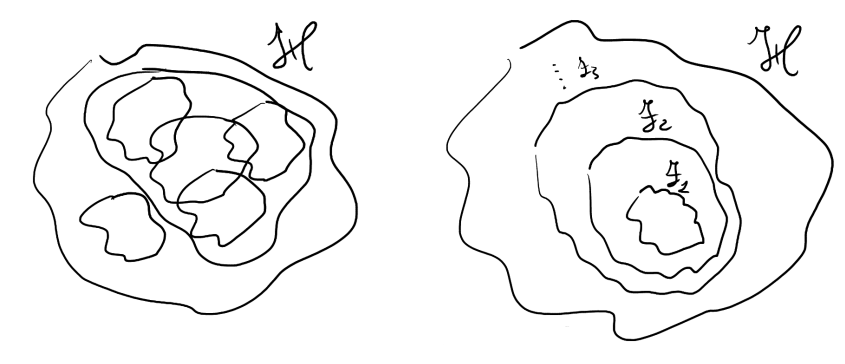
\includegraphics[width=.7\linewidth]{filtration}
	\caption{The first one is not a filtration, the second is for $T=\N^{*}$.}
	\label{fig:filtration}
\end{figure}
In figure \ref{fig:filtration} we can see how $\HS$ contains all events we are concerned with: it is built upon the \textit{experience} of the event we are facing. Take, for example, $\F_1$: it is much smaller than $\HS$ and if we say that a \rv{} is measurable with respect to $\F_1$ it means that we do not have much knowledge, but if we expand to $\F_2$ we are able to gain more knowledge about the \rv. If we interpret the index set $T$ as time we may actually think about filtrations as our knowledge of the phenomenon as time passes.
\begin{example}
	Consider a filtration generated by a stochastic process.
	Let $X={(X_{t})}_{t\in T}$. Of course each $X_t$ takes value in the same state space. Define
	\[\F_t=\sigma{(X_s)}_{\substack{s\leq t\\s\leq T}}.\]
	Here we are generating a \sa{} from all the random variables from the beginning of time until $t$. Consider now the family of \sa{}s 
	\[\F={(\F_t)}_{t\in T}:\]
	this is a filtration. This means that for this stochastic process, as time passes, we are gaining more knowledge about $\HS$ through the \sa s.
\end{example}
\subsection{Independency for a finite class of sub-\sa s}
We already know the concept of independence between \rv s and the effect of independence with respect to the induced measure of probability. If we look at \cinlar, it actually introduces independence of \rv{}s through the independence of \sa s. To do so we need to introduce the concept of \emph{independency for a finite class of sub-\sa s}.
\begin{definition}
	Consider the class $\HS$ as the collection of sub-\sa s $\F$:
\[\HS=\left\{\F_1,\F_2,\ldots,\F_n\right\}\qquad\F_i=\text{sub-$\sigma$-algebra }\every i=1,\ldots,n.\]
$\HS$ is said to be an \emph{independency} if
\begin{equation}
	\ev[V_1\cdot V_2\cdot\ldots V_n]=\ev V_1\cdot\ev V_2\cdot\ldots\ev V_n\tag{($\star$)}\label{independency}
\end{equation}
for $\every$ \rv{} $V_1,V_2,\ldots,V_n$ belonging respectively to $\F_1,\F_2,\ldots,\F_n$.
\end{definition}
But what does this definition mean? The definition is given in the terms of what happens to the \rv s that are measurable with respect to the \sa s. If for each of them we get the factorization of the expectation, then our sub-\sa s are independency... and so, of course, are their algebras (all \sa s are algebras.)\\
This definition is valid only for a \textit{finite} class of sub-\sa s, but we can extend it to infinite classes (\cinlar's book extends it to countable collections of sub-\sa{s} and even to uncountable collections of sub-\sa s, so we shouldn't.). This definition, though, was just an intuition of the fact that independency of \sa s and independency of \rv s are \textit{not} unrelated, but are simply the same concept seen from two different points of view. 
\begin{proposition}
	Let $\F_1,\F_2\ldots,\F_n$ be sub-\sa s of $\HS$, with $n\geq 2$. For each $i\leq n$, let $\mathcal{C}_i$ be a $\pi$-system generating $\F_i$. Then the collection $\left\{\F_1,\F_2,\ldots,\F_n\right\}$ is an independency \underline{if and only if}
	\[\pr(H_1\cap H_2\cap \ldots\cap H_n)=\prod_{i=1}^{n}\pr(H_i)\qquad\every H_i\in\overline{\mathcal{C}}_i=\mathcal{C}_i\cup\{\Omega\},\;i=1,\ldots,n.\]
\end{proposition}
We need to have clear that there is not an unique starting point in defining the concept of independency, so all of them are quite equivalent. We will build upon this fact and see other deep relations between these notions\footnote{Can't wait.}.
\begin{proposition}
	Every partition of an independency is an independency.
\end{proposition}
Take, for example, the collection 
${(\F_t)}_{t\in T}$ of sub-\sa s and the partition ${(T_i)}_{i\in\N^*}$
 of $T$: these two together form the sub-collection of sub-\sa s $\F_{T_i}={(\F_t)}_{t\in T}$
  with $i\in\N^{*}$.
\begin{notation}
	\[\F_{T_i}=\bigvee_{j\in T_i}\F_j.\]
\end{notation}
We are interested in checking whether $(\F_{T_1},\F_{T_2},\ldots)$ (remember: they are all \sa s!) are an independency... and they are.
\begin{proposition}
The notion of independence between \rv s (taking values in general measurable spaces) is given in terms of independence of the \sa s generated by those \rv s.
\end{proposition}
\begin{example}
	Consider
	$X_1,X_2$ where $X_1$ takes values in $(E_1,\E_1)$ and $X_2$ takes values in $(E_2,\E_2)$. If we are concerned about independence of the vector $(X_1,X_2)$ we should look at the vector of the collection of generated \sa s $(\sigma X_1,\sigma X_2)$ and check whether it is an independency or not.
\end{example}
\begin{proposition}	Let $X_1,X_2,\ldots,X_n$ be random variables taking values respectively in $(E_i,\E_i)$ for $i=1,\ldots,n$. They are independent \ifonly{} 
	\[\ev\left[f_i\circ X_1,f_2\circ X_n,\ldots,f_1\circ X_n\right]=\ev f_i\circ X_1,\ev f_2\circ X_n,\ldots,\ev f_1\circ X_n\]
	for every $f_1,\ldots,f_n$ positive and measurable with respect to $\E_1,\ldots,\E_n$ respectively.
\end{proposition}
We need to prove this proposition. But before, just because we like it (like the little sluts we are), let's state an equivalent proposition. 
\begin{proposition}
Let $X_1,X_2,\ldots,X_n$ be \rv s taking values in $(E_i,\E_i)$ for $i=1,\ldots,n$ respectively. Then they form an independency \ifonly{} their joint distribution equals the product of their marginal distribution.
\end{proposition}
Well we already knew that... but thanks. Now we see more clearly how these two properties are basically the same thing.
\begin{fancyproof}
	We will prove the first proposition. We go back to formula of independence \ref{independency} and show that it holds $\every V_1,V_2,\ldots,V_n$ positive and measurable with respect to
	\[\sigma X_1,\sigma X_2,\ldots,\sigma X_n\]
	respectively. We know that \ref{independency} holds because of \bigskip\hyperref[teodelta]{Theorem $\Delta$}.\\ 
	We will now prove the second proposition. From the first proposition we know that:
	\begin{align*}
		&\int_{E_1\times\ldots\times E_n}\underbrace{\pi(\dx_1,\ldots,\dx_n)}_{\mathclap{\tiny\text{joint distribution of }(X_1,\ldots,X_n)}}f_1(x_1)\cdot\ldots\cdot f_n(x_n)\\
		=&\int_{E_1}\mu_1(\dx_1)f_1(x)\cdot\int_{E_2}\mu_2(\dx_2)f_2(x)\cdot\ldots\int_{E_n}\mu_n(\dx_n)f_n(x)\
	\end{align*}
	Plainly, considering positivity of $f_1,f_2,\ldots,f_n$, to have the above equality we obtain that
	\[\pi=\mu_1\times\mu_n.\]
\end{fancyproof}
You should convince yourself that the second proposition is just the first proposition rewritten. So, the independence of \rv s is very important and right now we will see an application.
\subsection{Sums of independent \rv s}
The simplest structure that we can construct with \rv is just adding them up. Let $X,Y$ be independent real-valued \rv s with distribution $\mu,\nu$ respectively. Then the distribution $\mu\star\nu$ of $X+Y$ (i.e. the effect of $\mu\star\nu$ over $f$) is given by
\[(\mu\star\nu)f=\ev f(X+Y)=\int_{\R}\mu(\dx)\int_{\R}\mu(\dy)f(x+y).\]
This is called the \emph{convolution} of the measures $\mu$ and $\nu$.\\
 So if we are asked to calculate the distribution it is interesting to choose a specific $f$ to see why the distribution is defined in this way: let us choose $f=\indi_{(-\infty,z]}(x+y)$ so that when we calculate the expectation we get
\begin{align*}
	\ev f(X+Y)&=\ev \indi_{(-\infty,z]}(X+Y)=\pr(X+Y\leq z)\\
	&=\int_{\R}\mu(\dx)\int_{\R}\nu(\dy)\indi_{(-\infty,z]}(x+y)\\
	&=\int_{\R}\nu(\dy)\int_{\R}\indi_{(-\infty,z-y]}(x)\mu(\dx)\\
	&=\int_{\R}\underbracket[0.6pt]{F_X(z-y)}_{\mathclap{\text{distribution function of }X}}\nu(\dy)
\end{align*}
Which is what, supposedly, we saw in our undergraduate course\footnote{I didn't see anything remotely similar to this in my economics degree but what do I know. Economics is not real anyway and economists should kill themselves NOW.}.
From this last series of equations we can also have a look to a special case where $X$ is absolutely continuous with respect to the Lebesgue measure with density $h(x)$:
\begin{align*}
	\pr(X+Y\leq z)&=\int_{\R}F_X(z-y)\nu(\dy)=\int_{\R}\nu(\dy)\int_{-\infty}^{z-y}h(t)\dt\\
	&\stackrel{w=t+y}{=}\int_{\R}\nu(\dy)\int_{-\infty}^{z}h(w-y)\dif w\\
	&=\int_{\infty}^{z}\underbrace{\int_{\R}h(w-y)\nu(\dy)}_{\text{density of} X+Y}\dif w.
\end{align*}
Further, if $Y$ is also absolutely continuous wuth density $g$ we get that the density of $X+Y$ becomes
\[\int_{\R}h(w-y)g(y)\dy\]
Which is the convolution formula for calculating the density of $X+Y$. 
For a further example see ex. 2.1.3 of \cinlar page 43 (convolution of Gamma densities).\par
We can further consider a sequence of \rv s ${(X_n)}_{n\in\N^{*}}$ and start adding them up:
\[S_n=X_1+X_2+X_3+\ldots+X_n\]
so we stop at a finite time. But the we have a new sequence, which is the sequence ${(S_n)}_{n\in\N^*}$ where $S_n$ is called \textit{partial sum}. The partial sum is in itself a \rv{}, made by little \rv s added up and this is why $S_n$ is also called \emph{random walk}. The question is, as always,
\begin{center}
	``Should we care?''
\end{center}
and while the answer is often
\begin{center}
	``No''
\end{center}
this time it actually is 
\begin{center}
	``Kinda''
\end{center}
which is probably the most astounding result of this whole course. This is one of the first kinds of real problems (albeit very simplistic) modeled through the use of \rv s. To do this we need the notion of \textit{tail \sa}.
\subsection{Tail \sa}
Did you think that we were about to dive into some interesting and useful practical applications of the The name alone suggests a concept of something away from us. Think of an experiment involving $n\geq 1$ trials, like the repeated roll of a die or toss of a coin. What matters is that we have a trial repeated infinite times and the result of all these trials (which are \rv s) makes up our experiment, which is a \rv{} in itself. \\
The experiment is defined on $(\Omega,\HS,\pr)$. Consider a sequence ${(\G_n)}_{n\in\N^{*}}$ of sub-\sa s of $\HS$ such that $\G_n$ is the information on $\HS$ revealed by the $n$-th trial. 
\begin{example}
	Imagine that the trials are given by the sequence of trials is given by
	\[{(X_n)}_{n\in\Nstar}\]
	and the sub-\sa s are defined by
	\[{(\sigma X_n)}_{n\in\Nstar}\]
\end{example}
So the \sa s generated by each $X_n$ are actually the \textit{trajectories} of the \rv s.\\
Imagine we are sitting a time $n$. Consider now $\G_m$ for $m>n$: I want to take the union of all these \sa s, but since I am not sure that we would end up with a \sa, I take the \sa{} of that union.
\[\tau_n=\sigma\left(\bigcup_{m>n}\G_m\right)=\bigvee_{m>n}\G_m.\]
This \sa{} depends on $n$ and it represents the \textit{information about the future}, since we are now sitting at the time point $n$. Remember that when we talk about \textit{revealed information} we are always talking about \sa s!
This object is a bit strange... it is about the information that models the future. What the fuck? We now want to take the intersection of the various $\tau_n$ (which is surely a \sa{} since we are intersecting):
\[\tau=\bigcap_n\tau_n.\]
This is now the \textit{information about the remote future}: we are doing the \textit{intersection}, not the \textit{union}! This is not exactly what happens in the future, but the information revealed by all the infinite trials in the future. The \sa{} $\tau$ is called \emph{tail \sa{}}. Remember that we always remain inside $\HS$.
\begin{example}
	Consider ${(X_n)_{n\in\Nstar}}$ and ${(\G_n)}_{n\in\Nstar}={(\sigma X_n)}_{n\in\Nstar}$. We have 
	\[S_n=\sum_{i=1}^{n}X_i.\]
	\begin{enumerate}[\circnum]
		\item consider the event
		\[\left\{\omega:\lim_{n}S_n(\omega)\text{ exists.}\right\}\]
		If we think about the tail \sa, it is the intersection of the \sa s after $n$: it is composed by events whose occurence is not influenced by the happenings in finite time! If we look at this event it consists of all the realization of the random walk until infinity: so if I were to remove the first $n$ \rv s in this sequence then the limit of this sequence wouldn't be affected: so this event \textit{belongs} to $\tau$.
		\item consider the set $B\in\B_{\R}$ and consider the event
		\[\left\{\omega :X_n(\omega)\in B\text{ i.o.}\right\}.\]
		``\textit{i.o.}'' means \textit{infinitely often}: this means that
		\[\left\{\omega :X_n(\omega)\in B\text{ i.o.}\right\}=\left\{\omega:\sum_n\indi_B\circ X_n(\omega)=+\infty\right\}.\]
		So we infinitely many $\indi$'s in $B$. Again, it is clear that this event belongs in the tail \sa{} because to test the divergence of the series $\sum_n\indi_B\circ X_n(\omega)$ we need to consider the behavior in the limit. We don't care what happens in finite time, so if we remove the contribution of the first $n$ \rv s:
		\[\left\{\omega :X_n(\omega)\in B\text{ i.o.}\right\}\in\tau.\]
		\item consider again $B\in\B_\R$ and consider 
		\[\left\{\omega: S_n(\omega)\in B\io\right\}.\]
		This event does not belong in $\tau$! Why? Let's consider a special case of $B=\{0\}$ and therefore we consider the event
		\[\left\{\omega:S_n(\omega)=0\io\right\}\]
		and we also specialize the ``jumps'':
		\[{(X_n)}_{n\in\Nstar}\text{ is i.i.d. with }\begin{array}{l}
			\pr(X_1=1)=p\\
			\pr(X_1=-1)=1-p
		\end{array}\]
		with $p\in[0,1]$. In this case $\left\{\omega:S_n(\omega)=0\io\right\}$ is not a tail event. Let's realize the sequence of the ``jumps'' choosing an $\omega$ such that
		\[X(\omega)=(+1,-1,+1,-1,+1,\ldots)\]
		Clearly $\omega\in\left\{\omega:S_n(\omega)=0\io\right\}$:
		\begin{figure}[H]
			\centering
			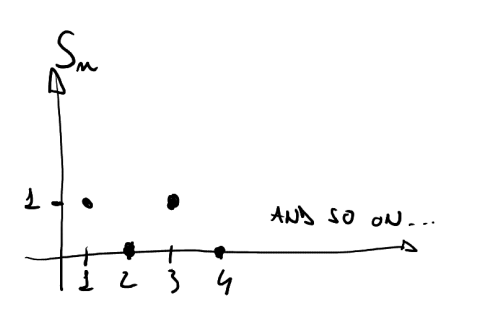
\includegraphics[width=0.5\linewidth]{screenshot006}
			\caption{The random walk randomly walking}
			\label{fig:screenshot006}
		\end{figure}
		Now we choose a different $\tilde{\omega}$ such that:
		\[X(\tilde{\omega})=(\color{SkyBlue4}+1,+1,+1,\color{black}+1,-1,+1,-1,\ldots)\]
		So in this case we have a ``ramp'' before the oscillation: $\tilde{\omega}\notin\left\{\omega:S_n(\omega)=0\io\right\}$! Try to make the same drawing: the walk will go up and the 0 will never be visited!\\
		Observe that $\omega$ and $\tilde{\omega}$ agree from the fourth coordinate on: but this means that the first events are decisive when it comes to determine whether a certain $\omega$ belongs to $\left\{\omega:S_n(\omega)=0\io\right\}$. This means that
		\[\left\{\omega:S_n(\omega)=0\io\right\}\notin\underbrace{\sigma(X_4,X_5,X_6,\ldots)}_{\mathclap{\text{\scriptsize We need more information to decide!}}}\implies\notin\tau_3\]
		So of course $\left\{\omega:S_n(\omega)=0\io\right\}\notin\tau$. The nature of the event is changed by a finite number of occurences...
		\item let $(X_1,X_2,\ldots)$ be independent and $S_n=\sum_{i=1}^{n}X_i$. Then
		\[\left\{\omega:\frac{S_n(\omega)}{n}\text{ converges (exists finite)}\right\}\in\tau.\]
		Consider 
		\[Z_1=\liminf_{n\to+\infty}\frac{S_n}{n},\;Z_2=\limsup_{n\to+\infty}\frac{S_n}{n}\]
		so that our event becomes
		\[\left\{\omega:Z_1(\omega)=Z_2(\omega)\right\}.\]
		Rewrite 
		\[ \frac{S_n}{n}=\underbracket[0.6pt]{\frac{1}{n}\sum_{i=1}^{m}X_i}_{{S_n}_1}+\underbracket[0.6pt]{\frac{1}{n}\sum_{i=m+1}^{n}X_i}_{{S_n}_2}\qquad m\leq n\]
		So that we ``split'' the partial sums in two sums before and after time $m$. We call these two partial sums ${S_n}_1$ and ${S_n}_2$. Note that when $n\to\infty$ then ${S_n}_1\to0$ and therefore $Z_1$ and $Z_2$ do not depend upon the first $n$ values of $(X_1,X_2,\ldots,X_m)$. Therefore 
		\[\left\{Z_1=Z_2\right\}\in\tau.\]
 	\end{enumerate}
\end{example}
\begin{theorem}
	\emph{Kolmogorov's 0-1 law}\\
	This is a theorem about independence. Let $\G_1,\G_2,\ldots$ be independent. Then
	\[\pr(H)=\begin{cases}
		0\\
		1
	\end{cases}\qquad\every H\in\tau.\]
\end{theorem}
So when the outcomes of a \rv{} are independent then the tail is made of almost sure or almost impossible events! The proof is short.
\begin{fancyproof}
	Remember that partition of independencies are independencies. Our independency is formed by the sub-\sa s $\G_1,\G_2,\ldots$ and our partition is
	\[(\G_1,\G_2,\ldots,\G_n,\tau_n).\]
	This is an independency $\every n\in\Nstar$. Since $\tau\subset\tau_n\;\every n$, then $(\G_1,\G_2,\ldots,\G_n,\tau)$ is an independency for each $n$. But since we now have an independency made of finite elements for each $n$ we have an independency of infinite components
	\[(\tau,\G_1,\G_2,\ldots)\]
	by definition of independency for countably infinite sequences. But again, if we partition that last independency we still get an independency:
	\[(\tau,\tau_0)\]
	is still an independency. Now consider two \sa s $H\in\tau,G\in\tau_0$. Since they are independent, we have that $\pr(H\cap G)=\pr(H)\pr(G)$. But since $\tau\subset\tau_0$ then we can choose $G=H$ and we get
	\[\pr(H)=\pr(H\cap H)=\pr(H)\pr(H)\]
	and the solution to this equation can only be 1 or 0.
\end{fancyproof}
We must remember that this is a special case where we have independence: this, in an experimental scenario, is modeled by independent trials. This result can be applied of concept of convergence. The idea is to build up instruments useful to the analysis of real \rv{} in their limits
\section{Convergence of \rv s and asymptotic behavior}
\subsection{Convergence of real sequences}
Let ${(x_n)}_n$ be a sequence in $\R,n\in\Nstar$. Then 
\[\liminf_nx_n=\sup_m\inf_{n\geq m}x_n\]
and the 
\[\limsup_n x_n=\inf_m\sup_{n\geq m}x_n.\]
Both are well defined numbers (and can possibly be infinity). We know that if
\[\liminf_nx_n=\limsup_n x_n\]
then the limit
\[\lim_{n}x_n\]
exists and the sequence is \emph{convergent}.
\begin{notation}
	Let $\varepsilon\in\R_+$. We let $\mathcal{i}_\varepsilon$  be the indicator function of $(\varepsilon,\infty)$:
	\[\mathcal{i}_\varepsilon(x)=\indi_{(\varepsilon,\infty)}(x)=\begin{cases}
		1, &x>\varepsilon\\
		0, &x\leq \varepsilon.
	\end{cases}\]
\end{notation}
We need two remarks about the convergence of $x_n$:
\begin{remark}
	\begin{itemize}
		\item Let ${(x_n)}_{n}$ be a sequence in $\R$. Then it converges to $x\in\R$ \ifonly{} 
		\[|x_n-x|\xrightarrow[n]{}0.\]
		\item Let ${(x_n)}_{n}$ be a sequence in $\R$. Then it converges to 0 \ifonly{}
		\[\every\varepsilon>0\exists k\text{ s.t. }x_{n}\leqslant\varepsilon\;\every n\geq k.\]
		This is the usual definition of the limit and it means that 
		\[x_n\xrightarrow[n]{}0\iff\sum_n\mathcal{i}_\varepsilon<+\infty\quad\every\varepsilon>0.\]
	\end{itemize}
\end{remark}
This means that we have a finite number of $x_{n}$ that are smaller than $\varepsilon$, so summing up the indicator function when we are in an interval larger than $\varepsilon$ we will get less than infinity. This concept connects the convergence of real-valued positive sequences with the convergence to 0 of real-valued positive sequences.\\
Further, the fact that
\[\sum_n\mathcal{i}_\varepsilon(x_n)<+\infty\iff\limsup_n\mathcal{i}_\varepsilon(x_n)=0\iff\lim_n\mathcal{i}_\varepsilon(x_n)=0\]
\begin{proposition}
	\emph{Cauchy's criterion}:\\
	Let ${(x_n)}_{n}$ be a sequence in $\R$. Then ${(x_n)}_{n}$ converges \ifonly{}
	\[\lim_{m,n\to\infty}|x_n-x_m|=0.\]
\end{proposition}
This criterion is interesting because it gives us a criterion to check whether the sequence converges without looking at the actual limit of the sequence...
\begin{proposition}
	If there exists a positive sequence ${(\varepsilon_n)}_n$ such that
	\[\sum_n\varepsilon_n<+\infty,\qquad\sum_n\mathcal{i}_{\varepsilon_n}(|x_{n+1}-x_n|)<+\infty\]
	Then ${(x_n)}_{n}$ is convergent.
\end{proposition}
This is another way to prove convergence: we just need to prove that the two series described above are finite.
\begin{definition}
	Given a sequence ${(x_n)}_{n}$, the sequence ${(y_n)}_{n}$ is said to be a \emph{subsequence of ${(x_n)}_{n}$} if there exists an increasing sequence ${(k_n)}_{n}\in\Nstar$ with $\lim_n k_n=\infty$ such that
	\[y_n=x_{k_n}\qquad\every n.\]
\end{definition}
So the subsequence is like a tool to extract elements from a sequence that are still a sequence!
\begin{notation}
	We will usually denote ${(y_n)}_n$ as ${(x_n)}_{n\in N}$ where $N={(k_n)}_n$.
\end{notation}
\begin{remark}
We say that ${(x_n)}_{n}$ converges \emph{along $N$} to $x$ if ${(x_n)}_{n\in N}$ converges to $x$. This basically means that we are extracting a subsequence from $x$ and check if it converges.
\end{remark}
\begin{remark}
	${(x_n)}_{n}$ converges to $x$ \ifonly{} every subsequence has the same limit $x$. The converse is also true!
\end{remark}
\begin{remark}
	Let ${(x_n)}_{n}$ be a bounded real sequence. Then it is always possible to extract from it a convergent subsequence. 
\end{remark}
So if we prove that ${(x_n)}_{n}$ is bounded we can always get a convergent subsequence...
\begin{proposition}
	\emph{Selection principle}:\\
	If every subsequence that has a limit has the same limit value $x$, then the sequence that we are considering tends to the same limit $x$
(that can be finite or infinite).
If the sequence is bounded and every convergent subsequence has the same limit $x$, then the sequence converges to $x$.
\end{proposition}
We now consider a lemma about the behavior of $\limsup$ and $\liminf$.
\begin{lemma}
	Let ${(x_n)}_{n}$ be a sequence of positive real numbers and let $\overline{x}_n=\frac{\sum_{i=1}^{n}x_i}{n}$. Let $N={(n_k)}_{k}$ be a subsequence of $\N$ with 
	\[\lim_k\frac{n_{k+1}}{n_k}=r>0.\]
	If ${(\overline{x}_n)}_{n}$ converges along $N$ to $x$ then
	\[\frac{x}{r}\leq\liminf_n\overline{x}_n\leq r\cdot x.\]
\end{lemma}
This is interesting because it gives us an idea of the fluctuation of the sequence of averages in terms of the behaviour of the subsequence $N$ and the limit $x$. We will make use of this lemma soon...
\begin{theorem}
	\emph{Helly's theorem}:\\
	For every sequence ${(c_n)}_{n}$ of distribution functions (this is not a real-valued sequence anymore) there exists a subsequence of distribution function ${(b_n)}_{n}$ and a limiting distribution function $x$ such that
	\[\lim_{n\to\infty}b_n(t)=c(t)\qquad\every t\text{ at which $c$ is continuous.}\]
\end{theorem}
\begin{lemma}
	\emph{Kronecker's lemma}:\\
	Let ${(x_n)}_{n}$ a real-valued sequence. let ${(a_n)}_{n}$ be a strictly positive sequence increasing to $\infty$. Finally, write 
	\[y_n=\frac{\sum_{k=1}^{n}x_k}{a_k}.\]
	Then if $(y_n)$ is convergent,
	\[\lim_{n\to\infty}\frac{1}{a_n}\sum_{k=1}^{n}x_k=0.\]
\end{lemma}
We are now ready to talk about what we actually care about in probability theory.
\subsection{Almost sure convergence}
\begin{definition}
	A real-valued sequence of \rv s ${(X_n)}_{n}$ on $(\Omega,\HS,\pr)$ is said to be \emph{almost sure convergent} (a.s. convergent) is the numerical sequence
	\[{\Big(X_n(\omega)\Big)}_{n}\]
	converges for almost all $\omega\in\Omega$. \\
	It is said to converge to $X$ if $X$ is an almost sure real-valued \rv{} and 
	\[\lim_{n\to\infty}X_n(\omega)=X(\omega)\]
	for almost all $\omega\in\Omega$.
\end{definition}
Let us define
\[\Omega_0=\left\{\omega\in\Omega:\liminf_n X_n(\omega)=\limsup_n X_n(\omega)\right\}.\]
Of course this is an event and we note that ${(X_n)}_{n}$ is almost sure convergent \ifonly{} $\Omega_0$ is an almost sure event (i.e. $\pr(\Omega_0)=1$).
\begin{theorem}
	\emph{Characterization of almost sure convergence}:\\
	A sequence of real valued \rv s ${(X_n)}_{n}$ converges to $X$ almost surely \ifonly{}, for every $\varepsilon>0$,
	\begin{equation}
		\sum_n\mathcal{i}_\varepsilon\circ|X_n-X|<\infty\tag{$\star\star$}\label{charconvsurealmost}
	\end{equation}
	almost surely.
\end{theorem}
\begin{fancyproof}
	Implication ($\implies$).\\
	Start from the fact that 
	\[X_n\to X\;\text{a.s.}\]
	Write $Y_n=|X_n-X|$: for every $\omega\in\Omega$, by the analogous result for real sequences, we have that 
	\[\sum_n\mathcal{i}_\varepsilon\circ Y_n(\omega)<\infty\qquad\every\varepsilon>0\]
	and therefore (\ref{charconvsurealmost}) holds.\\
	Then there is the converse implication ($\impliedby$).\\
	Let (\ref{charconvsurealmost}) hold and let us consider ${(\varepsilon_k)}_{k}$ be a strictly decreasing sequence converging to 0. Also, let
	\[N_k=\sum_n\mathcal{i}_{\varepsilon_k}\circ|X_n-X|.\]
	Then
	\[\pr(N_k<\infty)=1\qquad\every k\]
	and this is true because (\ref{charconvsurealmost}) holds! Now note that 
	\[\varepsilon_{k+1}<\varepsilon_k\implies\mathcal{i}_{\varepsilon_{k+1}}\geq\mathcal{i}_{\varepsilon_k}\implies N_{k+1}\geq N_{k}.\]
	But now we have to pay attention to the nature of the events involved: consider the event
	\[\left\{N_k<+\infty\right\}\qquad\every k.\]
	The sequence $\left(\left\{N_k<+\infty\right\}\right)_{k}$ decreases with $k$ towards the intersection
	\begin{align*}
		\bigcap_k\left\{N_k<+\infty\right\}&=\left\{\omega\in\Omega:\sum_n\mathcal{i}_\varepsilon\circ Y_n(\omega)\quad \every\varepsilon>0\right\}\\
		&=\Omega_0.
	\end{align*}
	Hence we want to evaluate
	\[\pr(\Omega_0)=\pr(\lim_k\left\{N_k<+\infty\right\})=\underbracket[0.6pt]{\lim_k\pr(N_k<+\infty)}_{\text{sequence of 1}}\]
	Where the last equality is true because of sequential continuity. So $\every \omega \in \Omega_0$ we have $X_n(\omega)\to X(\omega)$ which is the definition of almost surely convergence.
\end{fancyproof}
Let's study more what happens in the limits of these random walks. Remember that Kolmogorov's 0-1 law tells us something nice: if all the \rv s are independent then events in the asymptotic future will either be certain or impossible. But we know nothing about situations in which \rv s are dependent...
\subsection{Borel-Cantelli Lemmas}
Let ${(H_n)}_{n}$ be a sequence of events. Imagine evaluating the probability of all these events: we would end up with a sequence of real numbers. We may ask ourselves how the sum of the probability behaves.
\begin{theorem}
	\emph{First Borel-Cantelli Lemma}
	Let ${(H_n)}_{n}$ be a sequence of events. Then
	\[\sum_n\pr(H_n)<+\infty\implies\sum_n\indi_{H_n}<+\infty\quad\text{a.s.}\]
\end{theorem}
Remember that the second sum is equivalent to
\[\pr(H_n\io)=0\qquad\text{or}\qquad\pr(\limsup_n H_n)=0.\]
If you want to know more see \cinlar page 101.
Why do we need it to be almost surely? Well, the sum $\sum_n\indi_{H_n}$ contains an indicator of events (which is nothing else but a Bernoulli \rv) so it is in itself a \rv. So we are asking yourself whether the sum converges \textit{almost surely}. This theorem is important because if we can sum the probabilities then we can directly infer information about the presence of events! Let's see the proof\footnote{Professor Polito says that we should as interested in the result as in the proof. I do not agree and wish to die.}.
\begin{fancyproof}
	Denote
	\[N=\sum_n\indi_{H_n}\]
	So that
	\[\sum_n\pr(H_n)=\ev N.\]
	Our claim now becomes:
	\begin{center}
		``If $\ev N<+\infty$ then $N<\infty$ almost surely.''
	\end{center}
	But this is obvious: if the expectation is finite then the \rv{} is finite almost surely (mening that the support is finite).
\end{fancyproof}
That's it? That was cool and all. But let's see the first Borel-Cantelli lemma in action in the next proposition.
\begin{proposition}
	Let
	\[\sum_n\pr(|X_n-X|>\varepsilon)<+\infty\qquad\every\varepsilon>0.\]
	Then 
	\[X_n\xrightarrow[]{\text{a.s.}}X.\]
\end{proposition}
Here we are checking the convergence of the sum of a sequence of real numbers and we are given a result on \rv s. This is pretty neat!
\begin{fancyproof}
	Consider
	\[H_n=\left\{|X_n-X|>\varepsilon\right\}.\]
	Then, we apply Borel-Cantelli Lemma and we calculate
	\[\sum_n\indi_{\left\{|X_n-X|>\varepsilon\right\}}<+\infty.\]
	But now we are in the situation described by (\ref{charconvsurealmost}), so we know that
	\[X_n\convas X\]
\end{fancyproof}
So we can proof almost sure convergence by means of the application. So when we need to prove convergence always think about Borel-Cantelli lemmas!
\begin{proposition}
	Suppose that there exists a sequence ${(\varepsilon_n)}_{n}$ decreasing to 0 such that
	\[\sum_n\pr(|X_n-X|>\varepsilon_n)<+\infty.\]
	Then
	\[X_n\convas X.\]
\end{proposition}
So we don't need $\varepsilon$ to be constant, but just to be decreasing to 0.
\begin{proposition}
	Suppose that there exists a sequence of positive numbers ${(\varepsilon_n)}_{n}$ such that
	\[\sum_n\varepsilon_n<+\infty,\quad\sum_n\pr(|X_{n+1}-X_n|>\varepsilon_n)<+\infty\]
	Then $X_n$ converges almost surely.
\end{proposition}
Let's state again the two Borel-Cantelli lemmas side by side (and with a slightly different formulation).
\begin{theorem}
	\emph{Borel-Cantelli lemmas}\\
	\begin{enumerate}[a)]
		\item Let ${(B_n)}_{n}$ be a sequence of Bernoulli \rv s.
	\[\sum_n \ev B_n<+\infty\implies\sum_n B_n<+\infty\as\]
	\item If 
	\[\sum_n\ev B_n=\infty\text{ and }{(B_n)}_{n}\text{ are pairwise independent}\]
	then
	\[\sum_n B_n=+\infty\as\]
	\end{enumerate}
\end{theorem}
We will prove $b)$, the so-called ``divergence part''.
\begin{fancyproof}
	\begin{notation}
		\[p_n=\ev B_n,\quad a_n=\sum_{i=1}^n\ev B_i=\sum_{i=1}^{n}p_i\]
		and we get the partial sum and the limits
		\[S_n=\sum_{i=1}^{n}B_i,\quad S=\lim_n S_n\]
	\end{notation}
	First, we know that, due to pairwise independency in the hypothesis
	\[\var S_n=\sum_{i=1}^{n}\var B_i\]
	but we know that they are Bernoulli \rv s, so we can write the variance explicitly:
	\[\var S_n=\sum_{i=1}^{n}p_i(1-p_i)\leq\sum_{i=1}^{n}p_i=a_n\]
	where the inequality is just arithmetical calculations.\\
	 Second, fix $b\in(0,+\infty)$. We know that ${(a_n)}_{n}$ increases to $\infty$ by hypothesis:
	 \[\left(a_n-\sqrt{ba_n}\right)_n.\]
	 We are basically subtracting to $a_n$ something that goes to $\infty$ as well, but slower than $a_n$. So the sequence $\left(a_n-\sqrt{ba_n}\right)_n$ stays also increasing towards infinity. But if that is the case the event $\left\{S<+\infty\right\}$ is the limit of the increasing sequence of events
	 \[\left\{S<a_n-\sqrt{ba_n}\right\}.\]
	 Since $S_n\leq S\;\every n$ consider further the following modified sequence of events:
	 \[\left\{S_n<a_n-\sqrt{ba_n}\right\}\supset\left\{S<a_n-\sqrt{ba_n}\right\}.\]
	 Next, we also have
	 \[\left\{S_n<a_n-\sqrt{ba_n}\right\}\subset\left\{|S_n-a_n|>\sqrt{ba_n}\right\}.\]
	 Now, let's switch to the probability point of view. Remember that the events are included one in the other so we can think about weak inequalities of probabilities.
	 \[\pr(S<a_n-\sqrt{ba_n})\leq\pr(S_n<a_n-\sqrt{ba_n})\leq\pr(|S_n-a_n|>\sqrt{ba_n})\]
	 and we take the $\limsup_n$:
	 \[\limsup_n\pr(S<a_n-\sqrt{ba_n})\leq\limsup_n\pr(|S_n-a_n|>\sqrt{ba_n})\]
	 But the left hand side of the inequality is
	\begin{align*}
		 \limsup_n\pr(S<a_n-\sqrt{ba_n})&=\pr\left(\lim_{n}\left\{\pr(S<a_n-\sqrt{ba_n})\right\}\right)\\
		 &=\pr(S<\infty).
	\end{align*}
	We get, thus,
	\[\pr(S<+\infty)\leq\limsup_n\pr(|S_n-a_n|>\sqrt{ba_n}).\]
	But now we can apply Chebyshev's inequality:
	\[\pr(S<+\infty)\leq\limsup_n\frac{\var S_n}{b a_n}\]
	and we can now exploit the result we had reached before:
	\[\pr(S<+\infty)\leq\limsup_n\frac{\var S_n}{b a_n}\leq\limsup_n\frac{\cancel{a_n}}{b\cancel{a_n}}=\frac{1}{b}.\]
	If we let $b\to\infty$ we should get the same result and immediately obtain
	\[\pr(S<+\infty)\leq\frac{1}{b}\xrightarrow[b\to\infty]{}0\]
	and hence
	\[\pr(S=+\infty)=1.\]
\end{fancyproof}
Damn. I hate this. Let's see an example about coin toss!
\begin{example}
	Imagine considering the probability of getting a head\footnote{...so no head? Imma head out.}:
	\[\pr(H)\in(0,1),\qquad\Omega=\left\{H,T\right\}^\infty.\]
	We are infinitely tossing coin and the probability of having head is always the same. Our probability space is thus the space of infinity sequences of $H$ and $T$. Consider a chunk of tosses and define $B_1$ as the first subsequence of length $k$, $B_2$ as the second subsequence of length $k$ and so on. So we get infinitely many chunks of length $k$.\\
	Fix
	\[s=(s_1,s_2,\ldots,s_k)\in\left\{H,T\right\}^k.\]
	Now consider the events
	\begin{align*}
		D_1=&\left\{B_1=s\right\}\\
		D_2=&\left\{B_2=s\right\}\\
		D_3=&\left\{B_3=s\right\}\\
		&\vdots
	\end{align*}
	and suppose further that the sequence $s$ has actually $m$ heads and $k-m$ tails. Then 
	\[\pr(D_i)=[\pr(H)]^m\cdot[\pr(T)]^{k-m}.\]
	Imagine we want to calculate the sum:
	\[\sum_i\pr(D_i)=+\infty.\]
	But now we can use the Borel-Cantelli lemma (point $b)$)! So we get that 
	\[\sum_i\indi_{D_i}=\infty\]
	which means that 
	\[\pr(D_1\io)=1\]
	or, in other words, for any given sequence of $k$ outcomes we observe it infinitely often.
\end{example}
\subsection{Convergence in probability}
This definition is strictly related to almost sure convergence. In measure theory this is called \textit{convergence in measure} (makes sense...).
\begin{definition}
	Let ${(X_n)}_{n}$ be a sequence of real-valued random variables. Then ${(X_n)}_{n}$ converges to a further real-valued \rv{} \emph{in probability} if 
	\[\lim_n\pr(|X_n-X|>\varepsilon)=0\qquad\every\varepsilon>0.\]
\end{definition}
So this means that the probability of $X_n$ being at most $\varepsilon$ away from $X$ gets smaller and smaller as $n$ gets bigger. It is quite different than the notion of almost sure convergence... and it depends heavily on the probability measure $\pr$!
What we get now is a sequence of probabilities that we need to evaluate. 
\begin{example}
	Consider
	\[\Omega=[0,1],\;\HS=\B_{[0,1]},\;\pr=\underbracket[0.6pt]{\leb}_{\mathclap{\text{Lebesgue measure}}}.\]
	Consider the sequence of \rv s
	\[X_1,X_2,X_3,\ldots\]
	to be indicators of $(0,1],(0,\frac{1}{2}],(\frac{1}{2},1],(0,\frac{1}{3}],(\frac{1}{3},\frac{2}{3}],(\frac{2}{3},1],\ldots$ respectively.\\
	Then $\every\varepsilon>0,\varepsilon\in(0,1)$, $\pr(X_n>\varepsilon)$ forms the sequence
	\[(1,\frac{1}{2},\frac{1}{2},\frac{1}{3},\frac{1}{3},\frac{1}{3},\ldots)\xrightarrow[n\to\infty]{}0.\]
	Hence 
	\[X_n\convpr0.\]
	However,
	\[X_n(\omega)=\begin{cases}
		0\\		1
	\end{cases}\qquad\every\omega\in\Omega\]
	and therefore we have that 
	\[\liminf_n X_n=0,\;\limsup_n X_n=1\]
	and we do not have almost sure convergence... So \[\Omega_0=\left\{\omega\in\Omega:\liminf_n X_n(\omega)=\limsup_n X_n(\omega)\right\}\] is empty!
\end{example}
But how are these two different types of convergence related?
\begin{theorem}
	\emph{Characterization theorem for convergence in probability}. 
	\begin{enumerate}[label=\textit{\roman*})]
		\item \label{ehehe} if ${(X_n)}_{n}$ converges to $X$ almost surely, then it converges to $X$ in probability;
		\item \label{ehehe2} if ${(X_n)}_{n}$ converges in probability to $X$, then it has a subsequence converging to the same \rv{} $X$ almost surely;
		\item \label{ehehe3} if every subsequence of the main sequence has a further subsequence converging to $X$ almost surely, then the main sequence converges to $X$ in probability.
	\end{enumerate}
\end{theorem}
We will only prove point \ref{ehehe} because it is the most useful.
\begin{fancyproof}
	Let $X_n>0\;\every n$ and $X=0$: this means replacing $|X_n-X|$ with $X_n$ (as long as $X_n$ is positive and converges to 0). Recall the definition of indicator $\mathcal{i}_\varepsilon+\indi_{(\varepsilon,\infty)}$ and define
	\[p_n=p_n(\varepsilon)=\ev[\underbracket[0.6pt]{\mathcal{i}_\varepsilon\circ X_n}_{\mathclap{\text{Bernoulli r.v.}}}]=\pr(X_n>\varepsilon).\]
	Here we switch between expectation and probability because of \hyperref[expprob]{the property of expectations with indicator functions in this theorem}. We know that $X_n\convas 0$. Fix $\varepsilon>0$: now we have
	\[\indi_\varepsilon\circ X_n\convas0.\] Now take the expectation
	\[p_n=\ev\mathcal{i}_{\varepsilon}\convas0\]
	Hence
	\[\pr(X_n>\varepsilon)\xrightarrow[n\to\infty]{}0\]
	that is to say
	\[X_n\convpr0\]
\end{fancyproof}
\begin{proposition}
	Let $f:\R\mapsto\R$ be continuous. Then if $X_n\convpr X$ in probability then
	\[f(X_n)\convpr f(x)\]
	That is to say $f\circ N_n\convpr f\circ X$.
\end{proposition}
\begin{fancyproof}
	We know that $X_n\convpr X$. Let $N$ be a subsequence of $\Nstar$. Then $X_n\convpr X$ along $N$. For the point \refeq{ehehe2} of the previous theorem there exists a subsequence $N'$ along which the convergence takes place almost surely:
	\[X_n\convas X.\]
	Then along $N'$
	\[f\circ X_n\convas f\circ X\]
	for the continuity of $f$: looking at the limit of $f$ we exploit the continuity of $f$:
	\[\lim f\Big(X_n(\omega)\Big)=f\Big(\lim X_n(\omega)\Big).\] So saying that $f$ is continuous is enough to prove the convergence of its composition with $X$.\\
	Now by point \ref{ehehe3} of the previous theorem we conclude that 
	\[f\circ X_n\convpr F\circ N.\]
\end{fancyproof}
\begin{remark}
Convergence in probability is preserved under arithmetic operations. 
\end{remark}
So, for example if we have $X\convpr X$ and $Y_n\convpr Y$ then ${(X_n+Y_n)}_{n}\convpr X+Y$.\\
We will now introduce a metric for convergence in probability: since we are talking about \textit{distance}, we may think\footnote{A remark that reeks of overestimation.} that this has something to do with \textit{metric spaces}, where we measure the distance between different objects. Indeed there is a connection between measure spaces and metric spaces...\par
Let us introduce now a metric for convergence in probability. If we want to calculate a metric between \rv s $X$ and $Y$ we can define the following metric:
\[d(X,Y)=\ev(|X-Y|\wedge1).\]
\begin{remark}
	\begin{enumerate}[\circnum]
		\item $d(X,Y)=0 \iff X=Y\as$
		\item $d(X,Y)+d(Y,Z)\geq d(X,Z).$
	\end{enumerate}
	$d$ is a metric on the space of real-valued \rv s if $X$ and $Y$ are indentified as the same \rv{} if $X=Y$ almost surely.
\end{remark}
\begin{proposition}
	\[ X_n\convpr X\iff d(X_n,X)\xrightarrow[n\to\infty]{}0. \]
\end{proposition}
Instead of proving this version, we will prove a slightly different version of the proposition, that is:
\begin{theorem}
	$$X_n\convpr X\iff\lim_{n\to\infty}\ev\left[\frac{|X_n-X|}{1+|X_n-X|}\right]=0$$
\end{theorem}
\begin{fancyproof}
	Without losing generality we fix $X=0\as$ We are concerned about the following claim:
	\[X_n\convpr 0\iff\lim_{n\to\infty}\ev\left[\frac{|X_n|}{1+|X_n|}\right].\]
	$(\implies)$ Suppose that $X_n\convpr 0$. This means that 
	\[\lim_{n\to\infty}\pr(|X_n|>\varepsilon)=0,\qquad\every \varepsilon>0.\]
	Note that
	\[\frac{|X_n|}{1+|X_n|}\leq\frac{|X_n|}{1+|X_n|}\indi_{\left(|X_n|>\varepsilon\right)}+\varepsilon\indi_{\left(|X_n|<\varepsilon\right)}\]
	Because if $|X_n|$ is smaller than $\varepsilon$ then also the fraction above is smaller than $\varepsilon$ (duh). But we see that
	\begin{align*}
		\frac{|X_n|}{1+|X_n|}&\leq\underbracket[0.6pt]{\frac{|X_n|}{1+|X_n|}}_{<1}\indi_{\left(|X_n|>\varepsilon\right)}+\varepsilon\underbracket[0.6pt]{\indi_{\left(|X_n|<\varepsilon\right)}}_{\leq1}\\
		&\leq\indi_{(|X_n>\varepsilon|)}+\varepsilon
	\end{align*}
	Then take the expectation:
	\[\ev\left[\frac{|X_n|}{1+|X_n|}\right]\leq\underbracket[0.6pt]{\ev\indi_{(|X_n>\varepsilon|)}}_{\pr(|X_n|>\varepsilon)}+\varepsilon=\]
	and the limit
	\[\lim_{n\to\infty}\ev\left[\frac{|X_n|}{1+|X_n|}\right]\leq\varepsilon\]
	Because we know that $\pr(|X_n|>\varepsilon)$ goes to 0 as $n$ gets larger. But since $\varepsilon$ is chosen arbitrarily, then
	\[\lim_{n\to\infty}\ev\left[\frac{|X_n|}{1+|X_n|}\right]=0.\]
	$(\impliedby)$ Let 
	\[\lim_{n\to\infty}\ev\left[\frac{|X_n|}{1+|X_n|}\right]=0.\]
	We want to prove convergence in probability. Note that $f(x)=\frac{x}{1+x}$ is strictly increasing and therefore I can write the following inequality:
	\[\frac{\varepsilon}{1+\varepsilon}\indi_{(|X_n>\varepsilon|)}\leq\frac{|X_n|}{1+|X_n|}\leq\indi_{(|X_n>\varepsilon|)}\leq\frac{|X_n|}{1+|X_n|}.\]
	Now take the expectation and the limit for $n\to\infty$:
	\[[\frac{\varepsilon}{1+\varepsilon}\lim_{n\to\infty}\pr(|X_n|>\varepsilon)\leq\lim_{n\to\infty}\ev\left[\frac{|X_n|}{1+|X_n|}\right]=0\]
	where the last ``=0'' is by hypothesis. Since $\varepsilon$ is chosen arbitrariliy then
	\[\lim_{n\to\infty}\pr(|X_n|>\varepsilon)=0\]
	so we have proven the converse implication.
\end{fancyproof}
We said before that $X_n$ converges in probability to $X$ if the metric $d(X_n,X)\xrightarrow[n\to\infty]{}0$. The last proof refers to the function $f(x)=\frac{|x|}{1+|x|}$ but the same holds for every bounded, non decreasing, continuous function $g$ on $\R_+$ with $g(0)=0,g(x)>0\;\every x>0$. For example, $g(x)=|x|\wedge 1$ (which is similar to the metric we estabilished before).
\subsection{Convergence in $L^{p}$ spaces}
Let's start with the proper definition.
\begin{definition}
	A sequence ${(X_n)}_{n}$ of real-valued \rv s is said to be convergent to the real-valued \rv{} $X$ in $L^{p}$ if, for each $n$, $X_n\in\lp,X\in\lp$ and
	\[\lim_{n\to\infty}\ev|X_n-X|^{p}=0.\]
	\begin{revise}
		Recall the $p$-norm of $X$:
		\[\norm{X}_{p}=\left(\ev|X|^{p}\right)^{\frac{1}{p}}.\]
	\end{revise}
\end{definition}
Then $\lp$ is a normed vector space if we identify all the \rv s that are almost surely equal as one single \rv: this means that the norm works up to an equivalence class (if $A$ and $B$ are equal a.s. then for \textit{us} they are the same \rv{} as long as we work in $\lp$). In this case, the $\lp$-convergence is to be written as
\[
\lim_{n\to\infty}\norm{X_n-X}_{p}=0.
\]
\begin{remark}
	What happens if we have two different sequences converging to the same limit in $\lp$? If ${(X_n)}_{n}$ converges to $X$ in $\lp$ then $X$ is unique (up to equivalence).
\end{remark}
\begin{fancyproof}
	Consider
	\begin{align*}
		X_n&\convlp X\\
		X_n&\convlp Y
	\end{align*}
	\begin{revise}
		Recall the Minkowsky's inequality
		\[\norm{X-Y}_{p}\leq\norm{X-X_n}_{p}+\norm{X_n-Y}_{p}\xrightarrow[n\to0]{}0\]
	\end{revise}
	But both $\norm{X-X_n}_{p}$ and $\norm{X_n-Y}_{p}$ tend to 0 as $n\to\infty$, we have that
	\[X=Y\as\]
\end{fancyproof}
So, since they are the same \rv{} in $\lp$ then they differ only for elements of measure 0. 
\begin{remark}
	\[ X_n\convlp X\implies X_n\convpr X.\]
\end{remark}
This is quite strong! Convergence in $\lp$ is stronger! I wish the same could be said of my will to live.
\begin{fancyproof}
	We use Markov's inequality:
	\[\pr(|X_n-X|>\varepsilon)\leq\left(\dfrac{1}{\varepsilon}\right)^{p}\ev|X_n-X|^{p}\xrightarrow[n\to0]{}0\]
\end{fancyproof}
But is the converse true? NO IT IS NOT IT IS NOT TRUE IT IS A LIE. Consider this counterexample:
\begin{example}
	We show that the converse of what it is stated in the previous remark does NOT hold in general. Consider $\Omega=[0,1],\HS=\B_{[0,1]},\pr=\leb$. Consider ${(X_n}_{n}$ a sequence of indicators of the intervals
	\[(0,1],\left(0,\dfrac{1}{2}\right],\left(\dfrac{1}{2},1\right],\left(0,\dfrac{1}{3}\right],\left(\dfrac{1}{3},\dfrac{2}{3}\right],\left(\dfrac{2}{3},1\right],\ldots\]
	Note that we already proved that this sequences converges to 0 in probability. Note, moreover, that $X_n\convlp0$ because $\ev|X_n|$ forms the sequence $$\left(1+0\cdot p,1\cdot p+0\cdot q,\ldots\right)=\left(1,\frac{1}{2},\frac{1}{2},\frac{1}{2},\frac{1}{3},\frac{1}{3},\frac{1}{3},\ldots\right)$$ (remember that our $\pr$ is the Lebesgue measure, which is the length of the interval(). This sequence goes to zero, clearly.\\
	Now let's modify the sequence of \rv s:
	\[{(\hat{X}_{n})}_{n}=(X_1,2X_2,2X_3,3X_4,3X_5,3X_6,\ldots)\]
	and evaluate
	\[\pr(\hat{X}_n>\varepsilon)=\ev |X_n|\]
	because for indicators our probability coincides with the expectation. Now take the limit and see whether $(\hat{X}_{n})\convpr0$. However, if we do the calculations we get
	\[\ev|\hat{X}_{n}|=1\qquad\every n.\]
	Hence
	\[\hat{X}_{n}\not\xrightarrow[]{L^{1}}0\]
	so there exists a $p$ for which $\hat{X}_{n}$ does not converge to 0.
\end{example}
\begin{theorem}
	\emph{Characterization theorem for convergence in $L^1$}.\\
	Let ${(X_n)}_{n}$ be a sequence of real-valued \rv s then the following are equivalent:
	\begin{enumerate}[\circnum]
		\item ${(X_n)}_{n}$ converges in $L^{1}$;
		\item ${(X_n)}_{n}$ converges in probability and is uniformly continuous;
		\item ${(X_n)}_{n}$ is Cauchy for the $L^{1}$-convergence:
		\[\lim_{m,n\to\infty}\ev|X_m-X_n|=0.\]
	\end{enumerate}
\end{theorem}
\begin{proposition}
	\[X_n\xrightarrow[]{L^{1}}X\implies\lim_{n\to\infty}\ev X_n Y-\ev XY\]
	And this is true for every bounded \rv{} $Y$.
\end{proposition}
So it is not true in generale, but requires boundedness. Quite a strict need. See what I did there?
\begin{remark}
	Setting $Y=1\as$ we get that
	\[X_n\xrightarrow[]{L^{1}}X\implies\lim_{n\to\infty}\ev X_n=\ev X.\]
\end{remark}
\subsection{Weak convergence and convergence in distribution}
\begin{definition}
	The sequence of probability measures $\mu_1,\mu_2,\mu_3,\ldots$ on $\R$ is said to \emph{converge weakly} to $\mu$ if
	\[ \lim_{n\to\infty}\underbracket[0.6pt][4pt]{\mu_n f=\mu f}_{\mathclap{\text{integrals!!}}}\qquad\every f\in\mathbb{C}_{b}\]
	where $\mathbb{C}_b$ is the set of continuous and bounded functions from $\R$ to $\R$.
\end{definition}
So we are talking about convergence of probability measures and this is done through integrals. If the sequence of integrals converge towards a limiting integral then we say that the convergence happens for the \textit{sequence of measures}: this shouldn't come as a surprise, since YOU should remember that measures are what defines integrals. But remember that \rv s are ultimately characterized by their distributions (which are nothing else but probability measures!) so there must be some kind of connection between the distributions converging and their \rv s doing the same thing...\\
Consider a sequence ${(X_n)}_{n}$ of \rv s characterized by their sequence of distributions ${(\mu_{n})}_{n}$.
\begin{definition}
	The sequence ${(X_n)}_{n}$ is said to \emph{converge in distribution} to a limiting \rv{} $X$ with distribution $\mu$ if
	\[{(\mu_n)}_{n}\convw\mu\]
	that is to say if
	\[\lim_{n\to\infty}\ev f\circ X_n=\ev f\circ X \qquad\every f\in\mathbb{C}_{b}.\]
\end{definition}
\begin{notation}
	We usually denote convergence in distribution as
	\[X_n\convd X.\]
\end{notation}
\begin{remark}
	\begin{align*}
	X_n\convpr X&\implies X_n\convd X\\
	X_n\convlp X&\implies X_n\convd X\\
	X_n\convas X&\implies X_n\convd X\\
\end{align*}
\end{remark}
So we see: convergence in distribution is the weakest of them all. It is related to the behavior in the limit of the probability distribution... and just having the same probability distribution is not saying much about a \rv. Imagine that we have $Y\sim N(0,1)$ and $Z=-Y$. $Z$ is still a normal random variable, but clearly $Y(\omega)=a\implies Z(\omega)=-a$ so they are very different! But there is a special case...
\begin{remark}
	If $X_n\convd X$ and $X=a\as$ (degenerate \rv\footnote{Yeah I know some degenerates "random variables" around here.}). Then
	\[X_n\convpr X.\]
\end{remark}
What the actual fuck? Now convergence in distribution implies convergence in probability? I will end my own life RIGHT NOW!
\begin{fancyproof}
	Let us choose
	\[f(x)=\frac{|x-a|}{1-|x-a|}.\]
	Note that $f\in\mathbb{C}_{b}$. So we have
	\[\lim_{n\to\infty}\ev\frac{|X_n-a|}{1-|X_n-a|}=\ev f\circ X=\ev\frac{|a-a|}{1-|a-a|}=0.\]
	Lol! Now
	\[X_n\convpr a.\]
\end{fancyproof}
\begin{proposition}
	If $\mu$ and $\nu$ are probability measures on $\R$ and 
	\[\mu f=\nu f\qquad\every f\in\mathbb{C}_{n}\implies\mu=\nu.\]
\end{proposition}
\begin{definition}
	Take a distribution function $C(x)=\pr(X\leq x)$ and construct:
	\[q(u)=\inf\left\{x\in\R:C(x)>u\right\}.\]
	This is known as \emph{quantile function.}
\end{definition}
So the quantile functions finds the first point at which the distribution function exceeds the level $u$. This is just the compositional inverse of $C$, if we think about it.
\begin{proposition}
	\emph{Convergence of distribution functions and quantile functions.}\\
	The following points are equivalent:
	\begin{enumerate}[\circnum]
		\item ${(\mu_n)}_{n}\convw\mu$;
		\item take $C_n(x)=\pr(X_n\leq x)$ (distribution function: since it depends on $n$ we get a sequence of functions with respect to the index $n$). We have 
		\[C_n(x)\xrightarrow[]{}C(x)=\pr(X\leq x)\]
		for each point of continuity $x$ of the distribution function $C$;
		\item $q_n(u)\xrightarrow[]{}q(u)$ for every point of continuity $u$ of the quantile function $q$.
	\end{enumerate}
\end{proposition}
\begin{theorem}
	Consider a sequence ${(\mu_{n})}_{n}$ of probability measures such that 
	\[\mu_n\convw\mu,\]
	where $\mu$ is a further probability measure. The above convergence is equivalent to the existance of a probability space
	\[(\Omega',\HS',\pr')\]
	and some \rv s
	\[Y_1,Y_2,\ldots,Y\]
	on it such that the distribution of $Y_i$ is $\mu_i,i\in\N$ and of $Y$ is $\mu$ and we have that
	\[Y_n\convas Y\]
	on $(\Omega',\HS',\pr').$
\end{theorem}
This theorem is really important. We start with a sequence of weakly convergent probability measures, so we already know that on our initial space $(\Omega,\HS,\pr)$ there are some \rv s $X_1,X_2,\ldots,X$ with those (convergent) measures. These \rv s are still defined on $(\Omega,\HS,\pr)$, but this theorem tells us that there exists \textit{another space} $(\Omega',\HS',\pr')$ with other \rv s $Y_1,Y_2,\ldots,Y$ that are actually convergent almost surely! So if we have convergence in distribution and we want convergence almost surely we can have it, but at the cost of working in a different probability space.
\begin{figure}[h]
	\centering
	
\includegraphics[width=\textwidth]{screenshot007}
	\caption[Anon studies probability theory]{Anon realizes he was deceived by probability theory\protect\footnotemark.}
	\label{fig:screenshot007}
\end{figure}
\begin{corollary}
	\emph{Skorokhod representation}.\\
	$(X_n)\convd X$ \ifonly{} there exist \rv s $Y_1,Y_2,\ldots,Y$ on some probability space such that 
	\[Y_n\stackrel{d}{=}X_n\quad\every n, Y\stackrel{d}{=}x\;\text{and}\;Y_n\convas Y.\]
\end{corollary}
I could have stuffed another Metal Gear Solid joke here with the similarity between Skorokhod and Shagohod but I won't. Maybe. Anyway, the greentext in figure \ref*{fig:screenshot007} is enough for now. 
\begin{proposition}
	If $X_n\convd X$, the following are equivalent:
	\begin{enumerate}[\circnum]
		\item ${(X_n)}_{n}$ is uniformly integrable;
		\item $X_n$ and $X$ are integrable and
		\[\ev|X_n|\to\ev|X|.\]
	\end{enumerate}
\end{proposition}
But first let's introduce Fourier transform because... because fuck you. Let ${f_n}_{n}$ be the sequence of Fourier transforms of ${(\mu_{n})}_{n},\;\every n$:
\[f_n(r)=\int_{\R}e^{irx}\mu_n(\dx),\qquad r\in\R.\]
Remember that this is a function of $r$!
\begin{theorem}
	Let ${(\mu_n)}_{n}$, our sequence of probability measures, be weakly convergent \ifonly{}
	\[\lim_n f_n(r)=f(r)\qquad\every r\in\R\]
	and $f$ is continuous at 0. Moreover, $f$ is the transform of a probability measure $\mu$ on $\R$ and $\mu$ is the weak limit of ${(\mu_n)}_{n}$.
\end{theorem}
\footnotetext{Archived at \url{https://boards.4chan.org/sci/thread/16313511}}
With this notion we study weak convergence by means of the Fourier transform. Why would we want to do this? I am seriously at a loss for words. But dear Professor Polito comes to help! Look back at the equation for the Fourier transform of a measure $\mu$:
\[f(r)=\int_{\R}e^{irx}\mu(\dx),\qquad r\in\R\]
But this is an integral, which is... an expected value! consider $x$ as being the \rv{} $X$ and write
\[f(r)=\ev e^{irX}.\]
This is called the \emph{characteristic function of $X$} or the \emph{fourier transfrom of its measure}.
\begin{corollary}
	The sequence ${(X_n)}_{n}\convd X$ if
	\[\lim_n\ev e^{irX_{n}}=\ev e^{irX}\qquad r\in\R.\] 
\end{corollary}
But up to now we didn't say anything about the limiting random variables... to do so we need to introduce one of the main results in asymptotic analysis: the law of large numbers.
\subsection{The law of large numbers}
``Large numbers'' always mean ``what happens in the limit''. Let's start with the basic theorem.
\begin{theorem}
	Consider a sequence of real valued, pairwise independent \rv s $X_1,X_2,\ldots$ with finite common expectation and variance
	\[\ev X_n=a,\;\var X_n=b.\]
	Then:
	\begin{enumerate}[\circnum]
		\item $\overline{x}_{n}=\dfrac{\sum_{i=1}^{n}X_i}{n}\xrightarrow[]{L^{2}}a$;
		\item $\overline{x}_{n}\convpr a$;
		\item $\overline{x}_{n}\convas a$.
	\end{enumerate}
\end{theorem}
Huh. If you're anything like me this doesn't sound at all like the weak and strong laws of large numbers I've studied in the Economics degree. But again, what do I know. I'm sure we will find some surprising connections. Also we only need to prove the first and third point, because the second is implied by the third. Why does the theorem list it as the \textit{third} point, though? What are you trying to do, \textit{keeping me on the edge}?
\begin{fancyproof}
	\begin{enumerate}
		\item[\circled{1}] Define
		\[S_n=n\overline{X}_{n}\]
		and 
		\[\ev S_n=na,\;\var S_n=nb\]
		because of hypothesis of independence. Then
		\[\ev \overline{X}_{n}=a,\;\var \overline{X}_{n}=\frac{b}{n}.\]
		So if I look at
		\[
		\ev |\overline{X}_{n}-a|^{2}=\var \overline{X}_{n}\xrightarrow[n\to\infty]{}0
		\]
		because the variance is a constant divided by $n$.
		Hence 
		\[\overline{X}_{n}\xrightarrow[]{L^{2}}a\]
		\item[\circled{2}] This comes from Markov's inequality (which we already proved)...
		\item[\circled{3}] Assume $X_n\geq0$. This doesn't cause loss of generality because we can apply what we are going to prove to the positive and negative part of $X_n$ (which are both positive!).\\
		Define $N={(n_k)}_{k\in\Nstar}$ such that $n_k=k^2$. By Chebyshev's inequality we get
		\[\pr(|\overline{X}_{n}-a|>\varepsilon)\leq\frac{b}{\varepsilon^2k^2}\]
		since we are working on the subsequence $N$ where the variance of the \rv s $ \overline{X}_{n}$ is not $\frac{b}{n}$, but it is $\frac{b}{\text{value of subsequence}}$ which is $k^2$. Now sum and multiply by $\varepsilon^2$ to get
		\[\varepsilon^{2}\sum_{n\in N}\pr(|\overline{X}_{n}-a|>\varepsilon)\leq\sum_{k=1}^{\infty}\frac{b}{k^2}<\infty\qquad\varepsilon>0\]
		since the latter is a geometric series. But this tells us that $\sum_{n\in N}\pr(|\overline{X}_{n}-a|>\varepsilon)$ is a finite number and therefore... we can apply Borel-Cantelli lemma!
		\begin{revise}
			Borel Cantelli lemma:
			\[\sum_n\pr(H_n)<+\infty\implies\sum_n\indi_{H_n}<+\infty\quad\text{a.s.}\]
			and in particular if
			\[\sum_n\pr(|X_n-X|>\varepsilon)<+\infty\qquad\every\varepsilon>0.\]
			then 
			\[X_n\xrightarrow[]{\text{a.s.}}X.\]
		\end{revise}
		So 
		\[\overline{X}_{n}\to a\]
		along $N$. Let us call $\Omega_0$ the almost sure set on which the convergence takes place and
		$\every\omega\in\Omega_0$ we apply the following lemma (we have already proven)
		\begin{revise}
			If we have a sequence of positive numbers ${(x_n)}_{n}$ and consider the empirical sum $\overline{x}_{n}=\dfrac{\sum_{i=1}^{n}x_i}{n}$ and let $N=(n_k)\subset{\Nstar}$ with $\lim_k\dfrac{n_{k+1}}{n_{k}}=r>0$ (asymptotic linarity) and ${(\overline{x}_{n})}_{n}$ converges along $N$ to $x$ then
			\[\frac{x}{r}\leq\liminf \overline{x}_{n}\leq\limsup \overline{x}_{n}\leq rx.\]
		\end{revise}
		Note that 
		\[\frac{(k+1)^{2}}{k^{2}}\xrightarrow[k\to\infty]{}1\]
		and hence $\every \omega\in\Omega_0$ we have that
		\[\lim_{n\to\infty}\overline{X}_n(\omega)=a\qquad\every\omega\in\Omega_0\]
		with probability 1... which means, almost sure convergence!
	\end{enumerate}
\end{fancyproof}
This one was for sequence of \rv s with finite variance and expectations... But what if both are infinite?
\begin{proposition}
	Let ${(X_n)}_{n}$ be a sequence of positive independent and identically distributed (i.i.d.) \rv s with
	\[\ev X_1=+\infty.\]
	Consider also a further \rv{} $X$ distributed as $X_1$ (which means that they also have the same expectation). Then
	\[\overline{X}_{n}\convas\infty.\]
	\end{proposition}
This shouldn't be surprising, since we are given a sequence of positive \rv s with infinite expectation, that means that there is a lot of the probability mass resides in the tails. This causes the expectation to diverge when doing the integral. To prove this fact we must rely on the previous result.
\begin{fancyproof}
	We know that this behaviour is caused 
	by the tail of the distribution, so we are going to truncate the distribution.\\
	Fix $b\in\R$ and let $Y_n=X_n\wedge b$. So $X_n$ can have infinite support, while $Y_n$ is definitely bounded with the support finishing at $b$ (\emph{truncated \rv}). Let also
	\[\overline{Y}_{n}=\frac{\sum_{i=1}^{n}Y_i}{n}\]
	and note that 
	\[\ev Y_n=\ev(X_n\wedge b)<+\infty.\]
	By the previous theorem we know that 
	\[\overline{Y}_{n}\convas\ev(X\wedge n).\]
	The second result that we need is an ordering between $X_n$ and $Y_n$. Which is the largest? For each $n$ we have that $X_n\geq Y_n$ and this further implies that $\liminf_n\overline{X}_n\geq\lim_{n}\overline{Y}_{n}=\ev(X\wedge b)$ almost surely. This must be true for any choice of $b$, even if $b\to\infty$ and thus
	\[\ev(X\wedge b)\xrightarrow[b\to\infty]{}\ev X=+\infty\]
	using the monotone covergence theorem. That is,
	\[\liminf_n\overline{X}_{n}=+\infty\as\]
	Which basically means, since $\overline{X}_{n}$ is a non decreasing sequence, that
	\[\overline{X}_{n}\convas +\infty\]
\end{fancyproof}
There is a general theorem that puts together the last two theorems that we have seen so far:
\begin{theorem}
	\emph{Law of large numbers}:\\
	Let ${(X_n)}_{n}$ be a sequence of pairwise independent random variables with the same distribution as $X$. If $\ev X$ exists (infinite values are admitted!) then
	\[\overline{X}_n\xrightarrow[n]{\mathrm{a.s.}}\ev X.\]
\end{theorem}
This is an almost sure result and that's why we often call this theorem the \emph{strong law of large numbers} (SLLN).
Here are two useful inequalities:
\begin{itemize}
	\item \emph{Chebyshev's inequality}: here we are given a sequence of \rv s $X_n$ and build up the partial sums $S_n$. Here we \underline{must assume} that ${(X_n)}_{n}$ are i.i.d. and such that $\ev X_1=0.$
	\[\varepsilon^{2}\pr(|S_n|>\varepsilon)\leq\var S_n=\underbracket[0.6pt]{\ev S^{2}_n}_{\mathclap{\text{second moment!}}}\]
	so the variance gives us an upper bound of the probability $\pr(|S_n|>\varepsilon)$. If we don't have that $\ev X_1=0$ then $\var S_n\leq\ev S^{2}_{n}$ (the second moment is usually larger than the variance... still a good upper bound tho).
	\item \emph{Kolmogorov's inequality}: let ${(X_d)}_{n}$ be a sequence of independent \rv s such that $\ev X_n=0\;\every n$. Then $\every a\in(0,\infty)$
	\[a^{2}\pr\left(\max_{k\leq n}|S_k|>a\right)\leq\var S_n\]
	We are interested in the times from $1$ to $n$: the interesting thing is that the maximum value of the random walk is bounded by something that happens in time $n$.
\end{itemize}
We will prove this last inequality.
\begin{fancyproof}
	Fix $a>0,\;n\geq 1$ and define
	\[N{(\omega)}=\inf\left\{k\geq1:|S_k(\omega)|>a\right\}\qquad\every\omega.\]
	So for that specific $\omega$ we consider the first time for which the random walk exceeds the value $a$. Of course this time index $k$ depends on $\omega$, so $N(\omega)$ is a \rv. 
	Observe a couple of facts:
	\begin{enumerate}[1)]
		\item $N(\omega)=k\iff|S_k(\omega)|>a$  and $S_j(\omega)\leq a\quad\every j<k$. Then $\indi_{N=k}$ is a function of ($X_1,X_2,\ldots,X_n$) because I need the knowledge of $X$ up to $k$ to know whether $N=k$.
		\item For $k<n$ we define the following \rv s:
		\[U=S_k\indi_{N=k}\qquad\text{and}\qquad V=S_n-S_k.\]
		We know that $U$ depends on the first $k$ values of $X_n$, while $V$ depends only on $X_{k+1},X_{k+2},\ldots,X_{n}$. But this means that $U$ and $V$ are functions of independent \rv s, so $U\independent V$. Hence
		\[\ev UV=\ev U\underbracket[0.6pt]{\ev V}_{\mathclap{=0\text{ because }\ev X_n=0}}.\]
		Therefore
		\[\ev S_k\indi_{\{N=k\}}(S_n-S_k)=0.\]
		\item Consider $S^{2}_{n}$:
		\[S^{2}_{n}=\left[S_k+(S_n-S_{k})\right]^{2}\geq S_{k}^{2}+2S_{k}(S_n-S_k) \]
		The inequality is what I get if I neglect the negative term. So i am bounding what happens at time $n$ with what happens at time $k$. Note that $|S_k|^{2}>a^{2}$ when $\{N=k\}$ holds. Then 
		\[\ev S^{2}_{n}\indi_{N=k}\leq \underbrace{a^{2}\ev\indi_{\{N=k\}}}_{a^{2}\pr(N=k)}+2\underbrace{\ev S_{k}(S_n-S_{k})\indi_{\{N=k\}}}_{=0}\]
		and summing both sides for $k\leq n$ we get
		\[a^{2}\pr(N\leq n)\leq\ev S_n^{2}\indi_{\{N\leq n\}}\leq \ev S_{n}^{2}=\underbracket[0.6pt]{\var S_n}_{\mathclap{\text{because of independence}}}.\]
		Hence
		\[a^{2}\pr(N\leq n)\leq\var S_n\]
	\end{enumerate} 
	But we know that \[\pr(N\leq n)=\pr(\max_{k\leq n}|S_k|>a)\]
	So our proof is finished.
\end{fancyproof}
\begin{proposition}
	Let ${(X_n)}_{n}$ be independent and with mean 0. If
	\[\sum_n\var X_n<+\infty\implies\sum_{n}X_n<+\infty\as\]
\end{proposition}
\begin{proposition}
	Let ${(X_n)}_{n}$ be a bounded sequence of i.i.d. \rv s. If
	\[\sum_n(X_n-a_n)<+\infty\as\]
	for some sequence ${(a_n)}_{n}\subset\R$ then
	\[\sum_n\var X_n<+\infty.\]
\end{proposition}
\begin{theorem}
	\emph{Kolmogorov's 3-series theorem}.\\
	Let ${(X_n)}_{n}$ be independent \rv s. We have
	\[\sum_{n}X_n<+\infty\as\]
	\ifonly{} the following 3 series are convergent:
	\begin{enumerate}
		\item $\sum_n\pr(X_n\neq Y_n)$ where $Y_n=X_n\indi_{\{|X_n|<b\}}$;
		\item $\sum_n\ev Y_n$;
		\item $\sum_n\var Y_n$.
	\end{enumerate}
\end{theorem}
So: remember that expectation is a number, so the LLN tells us that $\overline{X}_{n}$ (a \rv) tends to $\ev X$ (a degenerate \rv): our variability gets lots as $n\to\infty$. This affects many characteristics of the \rv...
\subsection{Central limit theorem}
There are different versions of the Central limit theorem and we have probably already studied some of those: the most common in undergraduate courses is the \emph{De Moivre-Lapalce Central limit Theorem}.
\begin{theorem}
	Let ${(X_i)}_{i}$ be a sequence of i.i.d. real-valued \rv s with finite mean $\ev X_1=a$ and finite variance $\var X_1=b$. Then
	\[\mathscr{Z}_{n}=\frac{S_n-na}{\sqrt{nb}}\convd Z\sim N(0,1)\]
\end{theorem}
The usual way to prove this theorem is relying on characteristic function. If $a=0,b=1$ then $Z_{n}=\frac{S_n}{\sqrt{n}}$ where $Z_{n}$ is the sum of ``small'' indpendent \rv s $X_{n,1}=\frac{X_1}{\sqrt{n}},X_{n,2}=\frac{X_2}{\sqrt{n}},\ldots,X_{n,n}=\frac{X_n}{\sqrt{n}}$. All of them are ``small'' with respect to their original \rv{} $X_n$ because we are dividing by $\sqrt{n}$: they get smaller and smaller as $n\to\infty$ but overall, for each $n$, $Z_{n}$ has a stable mean $0$ and variance $1$. The general idea behind the CLT is exactly this: we divide all of these variables for the ``right amount'' so that the limit of our sequence of \rv s stays stable and does not become a degenerate limit.
\begin{definition}
	A \emph{triangular array} (Professor Polito calls it ``a nice object``) is an infinite matrix with a special structure:
	\[\left[X_{nj}\right]=\begin{bmatrix}
		X_{11}&X_{12}&X_{13}&\ldots\\
		X_{21}&X_{22}&X_{23}&\ldots\\
		X_{31}&X_{32}&X_{33}&\ldots\\
		\vdots&\vdots&\vdots&\ddots\\
	\end{bmatrix}\]
	where the entries are real-valued \rv s (so it is actually an infinite random metric). Furthermore, for each $n$ there exists an integer $k_{n}$ such that $X_{nj},j>k_{n}$. The sequence of indices ${(k_{n})}_{n}$ is increasing towards $\infty$.
\end{definition}
So the \rv s are equal to 0 to the right hand side of the index $k_n$ for each row. The first row has $k_1$, the second row is composed by $k_2>k_1$ (so there are more non-zero \rv s than in row 1) and so on. So it's not really a triangular matrix (there's no rule on \textit{how much} $k_{n}$ is larger than $k_{n-1}$) but it is ``basically'' triangular. \\
Now define
\[Z_{n}=\sum_{j}X_{nj} \qquad(j=1,2,\ldots,k_{n}).\]
Remember that even if we are summing infinite random variables only a finite number of them are non-zero. Now consider the assumption that the \rv s on each row are independent among them (there \textit{may} be dependence with \rv s in other rows.). With this structure in mind we can formalize the following formulation of the CLT:
\begin{theorem}
	\emph{Lyapunov Central limit Theorem}:\\
	Suppose $\ev X_{nj}=0\;\every n,j$ and $\var Z_{n}=1\;\every n$ and $\lim_{n}\sum_n\ev|X_{nj}|^{3}=0$. Then
	\[Z_{n}\convd Z\asstnr.\]
\end{theorem}
Here we have replaced the conditions on the \rv s with the condition $\lim_{n}\sum_n\ev|X_{nj}|^{3}=0$ which allows us to use the structure of the triangular array. To prove this theorem we need the following lemma:
\begin{lemma}
	\emph{Lindeberg's lemma}:
	Let $(Y_1,Y_2,\ldots,Y_k)$ be independent \rv s with mean zero and let $S=\sum_{j=1}^{k}Y_{j}$. Let us further assume that $\var S=1$. Let $f$ be a function which can be differentiated 3 times and let 
	$f',f'',f'''$ be bounded and continuous and such that
	\[|f'''|\leq x,\qquad c\in\R_+.\]
	Then for $Z\asstnr$
	\[|\ev f\circ S-\ev f\circ Z|\leq c\sum_{j=1}^{k}\ev|Y_{j}|^{3}\]
\end{lemma}
This means that if the hypotheses are met then the distance between $S$ and a normal \rv{} is bounded so we can approximate $S$ by means of a normal \rv{}. We will prove this lemma.
\begin{fancyproof}
	Let $Z_1,\ldots,Z_k$ be independent normal random variables with mean $\ev Z_{j}=\ev Y_{j}=0$ for $j=1,\ldots,k$ and variance $\var Z_{j}=\var Y_{j}$ for $j=1,\ldots,k$. Then construct
	\[T=\sum_{j=1}^{k}Z_j\sim N(0,\sum_{j=1}^{k}\var Z_{j}=\sum_{j=1}^{k}\var Y_{j}=1).\]
	So we know that $T$ is distributed as $Z$ (they are both $N(0,1)$) so $T\stackrel{d}{=}Z$ and since we are using the expectation of $Z$ we can replace $\ev f\circ Z$ with $\ev f\circ T$. So the Linderberg's lemma becomes
	\[|\ev f\circ S-\ev f\circ T|\leq c\sum_{j=1}^{k}\ev|Y_{j}|^{3}\]
	which we want to prove, to exploit the structure of T. Define now the \rv s $V_1,V_2,\ldots,V_k$ as follows:
	\[\begin{array}{c c l c}
		V_1&\text{s.t.}&S=V_1+Y_1\\
		V_2&\text{s.t.}&V_1+Z_1=V_2+Y_2\\
		&&\vdots\\
		V_j&\text{s.t.}&V_j+Z_j=V_{j+1}+Y_{j+1},&1\leq j<k\\
		&&\vdots\\
		V_k&\text{s.t.}&V_{k}+Z_{k}=T.\\
	\end{array}\]
	Note that 
	\begin{align*}
		V_{1}&=Y_{2}+Y_{3}+\ldots+Y_{k}\\
		V_{2}&=Z_1+Y_{3}+\ldots+Y_{k}\\
		V_{3}&=Z_1+Z_{2}+Y_{4}+\ldots+Y_{k}\\
	\end{align*}
	so the $Y$ get replaced by the $Z$ one at the time in the $V$. We can now focus on the following expression:
	\begin{align*}
		f\circ S-f\circ T&=f(V_1+Y_1)-f(V_{k}-Z_{k})\\
		&=f(V_{1}+Y_{1})+f(V_{2}+Y_{2})-\underbracket[0.6pt]{f(V_{2}+Y_{2})}_{f(V_1+Z_1)}+f(V_{3}+Y_{3})-\underbracket[0.6pt]{f(V_{2}+Y_{2})}_{f(V_2+Z_2)}+\\
		&+\ldots+f(V_{k}+Z_{k})\\
		&=\sum_{j=1}^{k}f(V_{j}+Y_{j})-\sum_{j=1}^{k}f(V_j+Z_j).
	\end{align*}
	Now take the expectation and the absolute value:
	\begin{align*}
		|\ev f\circ s-\ev f\circ t|&=\left|\sum_{j=1}^{k}\ev f(V_{j}+Y_{j})-\sum_{j=1}^{k}\ev f(V_j+Z_j)\right|\\
		&\leq\sum_{j=1}^{k}\left|\ev f(V_{j}+Y_{j})-\ev f(V_j+Z_j)\right|
	\end{align*}
	and now we only need to prove that 
	\[\left|\ev f(V_{j}+Y_{j})-\ev f(V_j+Z_j)\right|\leq c\ev|Y_{j}|^{3}.\]
	Let's write the Taylor formula for this function:
	\begin{equation*}
		f(v+x)=f(v)+f'(v)x+\frac{1}{2}f''(v)x^{2}+R_{2}(v,x)
	\end{equation*}
	where
	\begin{align*}
		R_{2}(v,x)&=\frac{1}{2}\int_{v}^{v+x}(v+x-t)_{2}f''(t)\dt\\
		&\leq \frac{1}{2}c\int_{v}^{v+x}(v+x-t)_{2}\dt=c\frac{x^{3}}{6}
	\end{align*}
	so that
	\[|	R_{2}(v,x)|\leq\frac{c}{6}|x|^{3}.\]
	We now have
	\begin{align*}
		f(V_j+Y_j)&=f(V_j)+f'(V_j)Y_j+\frac{1}{2}f''(V_{j})Y_{j}^{2}+R_2(V_j,Y_j)\\
		f(V_j+Z_j)&=f(V_j)+f'(V_j)Z_j+\frac{1}{2}f''(V_{j})Z_{j}^{2}+R_2(V_j,Z_j)\\
	\end{align*}
	and subtract side by side:
	\begin{equation*}
		f(V_j+Y_j)-f(V_j+Z_j)=(Y_j-Z_j)f'(V_j)+\frac{1}{2}f''(V_j)(Y^{2}_{j}-Z^{2}_{j})+R_2(V_{j},Y_{j})-R_2(V_{j},Z_{j}).
	\end{equation*}
	Now take the expectation 
	\begin{align*}
		\ev f(V_j+Y_j)-\ev f(V_j+Z_j)=&\frac{1}{2}\ev f''(V_j)(\underbrace{\ev Y^{2}_{j}-\ev Z^{2}_{j}}_{\mathclap{=0\text{ since they have same variance}}})+\ev\left[R_2(V_{j},Y_{j})-R_2(V_{j},Z_{j})\right]\\
		&=\ev\left[R_2(V_{j},Y_{j})-R_2(V_{j},Z_{j})\right].
	\end{align*}
	Now take the absolute value
	\begin{align*}
		\left|\ev\left[R_2(V_{j},Y_{j})-R_2(V_{j},Z_{j})\right]\right|&\leq\ev|\left[R_2(V_{j},Y_{j})\right]|+\ev\left[|R_2(V_{j},Z_{j})|\right]\\
		&\leq\frac{c}{6}\left(\ev|Y|^{3}+\ev|Z|^{3}\right)
	\end{align*}
	so that 
	\begin{equation*}
		|	\ev f(V_j+Y_j)-\ev f(V_j+Z_j)|\leq\frac{c}{6}\left(\ev|Y|^{3}+\ev|Z|^{3}\right).
	\end{equation*}
	Recall that $Z_j\sim N(0,b^{2})$ where $b^{2}=\ev Y^{2}_{j}$. We know that
	\[\ev|Z_j|^{3}=b^{3}\sqrt{\frac{8}{\pi}}\leq 2b^{3}\]
	and we also have 
	\[b=\left(\ev Y^{2}_{j}\right)^{\frac{1}{2}}\leq\left(\ev |Y_{j}|^{3}\right)^{\frac{1}{3}}\]
	Because $L^{2}$ norm is less or equal than $L^{3}$ norm (revise inclusions in $L^{p}$-spaces for different values of $p$). But this last inequality is equivalent to
	\[b^{3}\leq\ev|Y_{j}|^{3}\]
	which leads to
	\[\ev\left|Z_j\right|^{3}\leq2 b^{3}\leq2\ev\left|Y_j\right|^{3}.\]
	Finally we get
	\begin{align*}
		\left|\ev f(V_j+Y_j)-\ev f(V_j+Z_j)\right|&\leq\frac{c}{6}\left(\ev\left|Y_j\right|^{3}\right)\\
		&=\frac{c}{6}3\ev\left|Y_{3}\right|^{3}\\
		&=\frac{c}{2}\ev\left|Y_{3}\right|^{3}\leq c\ev\left|Y_{3}\right|^{3}.\\
	\end{align*}
\end{fancyproof} 
This was horrible, horrible. Truly an horrible experience and honestly useless proof. And we still have to prove Lyapunov's theorem. 
\begin{fancyproof}
	\emph{Lyapunov's CLT}. Recall
	\begin{equation*}
		Z_{n}=\sum_{j}X_{nj}\qquad Z\asstnr.
	\end{equation*}
	We are interested in evaluating the characteristic function.
	\begin{align*}
		e^{irZ_n}&=\cos rZ_n+i\sin rZ_n\\
		e^{irZ}&=\cos rZ+i\sin rZ.\\
	\end{align*}
	Consider now
	\begin{align*}
		\left|\ev e^{irZ_n}-\ev e^{irZ}\right|&=\left|\left(\ev\cos rZ_n-\ev\cos rZ\right)+i\left(\ev\sin rZ_n-\ev\sin rZ\right)\right|\\
		&\leq\left|\ev\cos rZ_n-\ev\cos rZ\right|+\underbracket[0.4pt]{|i|}_{1}\left|\ev\sin rZ_n-\ev\sin rZ\right|.
	\end{align*}
	By applying the above lemma  we obtain
	\begin{equation*}
			\left|\ev e^{irZ_n}-\ev e^{irZ}\right|\leq\sum_j|r|^{3}\ev|X_{nj}|^{3}+\sum_{j}|r|^{3}\ev|X_{nj}|^{3}
	\end{equation*}
	and this is possible since both sine and cosine are differentiable three times and they are bounded by 1 (so our $c=1$). Now, according to the hypotheses of Lyapunov's theorem, we need to take the limit considering the hypothesis that $\lim_{n\to\infty}\sum_j\ev|X_{nj}|^{3}=c$ and we obtain the claim. This theorem applies to all triangular arrays which include the one in the CLT.
\end{fancyproof}
WHY.
\section{Conditional expectations}
Are you comfortable with the concept of expectation? Well brace yourself buddy because we are going to fuck it up and reveal that normal expectations are just a particular case of conditional expectations.\\
Consider our dear old probability space $(\Omega,\HS,\pr)$, a $\overline{\R}$-valued \rv{} $X$, a sub-\sa{} $\F\in\HS$ where $\F$ is the space of $\F$-measurable\rv s taking values in $\overline{\R}$. Remember that $\F$ can be considered the body of information revealed by our \rv{}. Consider now the event $H$. Fix $\omega\in\Omega$ and pretend that our only knowledge of $\omega$ is that of the $\omega\in H$. First of all, remember that
\[\pr(A|B)=\frac{\pr(A\cap B)}{\pr(B)}=\frac{1}{\pr(B)}\int_A\indi_B\dpr\]
Evaluate our best estimate for $X(\omega)$, which may very well be the average of $X$ over $H$:
\begin{equation*}
	\frac{1}{\pr(H)}\int_H X(\omega)\pr(\dw)=\frac{1}{\pr(H)}\ev X\indi_H=\ev_H X.
\end{equation*}
If $\pr(H)=0$ then we allow any value for $\ev_H X$.
\begin{notation}
	We usually denote that quantity as $\ev(X|H)$ but \cinlar denotes it as $\ev_H X$.
\end{notation}
Another interesting way to look at this question is the following: conditional probability basically gives us a new probability measure while leaving the rest of the ``ingradients'' of the probability triplet unchanged. And it makes quite sense: we change the way we weigh a certain event. So if we want, for instance, to condition our probability measure to the event $B$ our probability space $(\Omega,\HS,\pr)$ becomes $(\Omega,\HS,\pr(\cdot|B))$. This also means that our expectation $\ev X=\int_\Omega X\dif\pr$ becomes $\ev_B X=\int_\Omega X\dif\pr(\cdot|B)$.
\begin{remark}
	This best estimate is ``best'' in the same sense as the expectation of $X$ is the best estimate of $X$ when we do not know anything about $\omega$. The unconditional case is retrieved if $H=\Omega$.
\end{remark}
\begin{remark}
	The quantity $\ev_H X$ is called \emph{conditional expectation of $X$ given the event $H$}.
\end{remark}
Up to now, nothing new. Let's go a step further. Now suppose that $\F$ is generated by a measurable partition ${(H_n)}_{n}$ of $\Omega$. Fix $\omega\in\Omega$ and consider the problem of building an estimate of the \rv{} $X(\omega)$ with only the body of information given by the partition/sub-\sa{} $\F$: we could construct a ``best estimate'' of $X(\omega)$ for every event $H_n$:
\begin{equation}
	\overline{X}(\omega)=\sum_{n}^{}\ev_{H_{n}}X\indi_{H_n}(\omega)\tag{♪}\label{bratsummer}.
\end{equation} 
So for every specific $\omega$ only one term of the sum will be different from 0: if $\omega_0$ belongs in $H_{0}$ then only $\ev_{H_{0}}X$ in the sum will be non-zero and $\overline{X}(\omega_0)=\ev_{H_{0}}X$. So in this sense we can summarize all the information available. So $\overline{X}(\omega)$ is a \rv{} that we will call \emph{conditional expectation of $X$ given $\F$} and we will write
\[\overline{X}=\ev_{\F}X\quad\text{or}\quad\ev\left[X|\F\right].\]
 So expectation of a \rv{} is a \textit{number}, while the conditional expectation with respect to a sub-\sa{} is a \textit{\rv{}}. 
 \begin{example}
 	Imagine we have $\Omega=(0,1),\HS=\B_{(0,1)},\pr=\leb$. Consider the partition of $\Omega$ given by $\F=\sigma\left(\left\{H_{1},H_{2},H_{3}\right\}\right)$. The wiggly line is the realization of our process $X(\omega)$.
\begin{figure}[H]
	\centering
	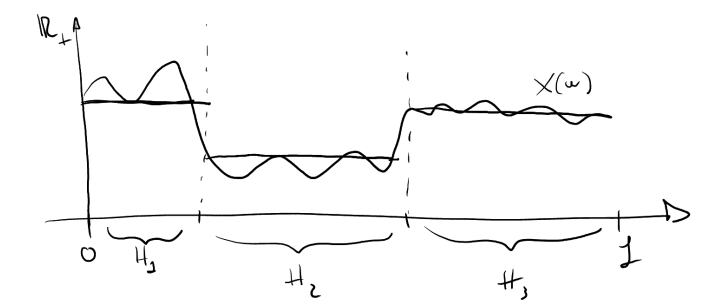
\includegraphics[width=0.8\linewidth]{screenshot008}
	\caption[Brat summer never ends]{♪ I think the apple is rotten right to the cooore}
	\label{fig:screenshot008}
\end{figure}
So according to our formula (\ref{bratsummer}) in our first partition $H_1$ we have a certain expected value (which is an average\footnotemark: expectation of a \rv{} is a number...) which is different from the value in the second partition an in the third.
 \end{example}
 \footnotetext{It's funny how this shit makes you really forget that the expected value is just the fucking average.}
 \subsection{Conditional expectation conditional on arbitrary \sa{}s}
Consider the following facts:
\begin{enumerate}
	\item $\overline{X}\in\F$: it is measurable with respect to $\F$ and this is clear from the definition \ref{bratsummer} of the \rv{} $\overline{X}$;
	\item we know that for each $V\in\F_{+}$ we have that
	\[\ev VX=\ev\xbar\]
	which is called \emph{projection property}.
	\begin{fancyproof}
		We start by letting $V=\indi_{H_n}$ for some fixed $n$ (and consider $\xbar=\ev_{H_{n}}X$). The statement becomes 
		\[\ev\indi_{H_{n}}X=\ev\indi_{H_{n}}\xbar.\]
		The left hand side reads
		\[\ev\indi_{H_{n}}X=\int_{\Omega}\indi_{H_{n}}(\omega)X(\omega)\pr(\dw)=\int_{H_{n}}X(\omega)\pr(\dw).\]
		The right hand side reads
		\begin{align*}
			\ev\left[\indi_{H_n}\cdot\frac{1}{\pr(H_{n})}\int_{H_{n}}X(\omega)\pr(\dw)\right]&=\frac{1}{\cancel{\pr(H_{n})}}\int_{H_{n}}X(\omega)\pr(\dw)\cancel{\pr(H_{n})}\\
			&=\int_{H_n}X(\omega)\pr(\dw).
		\end{align*}
		Now consider a general \rv{} $V\in\F_{+}$. Of course we have (for construction) 
		\[V=\sum_n a_{n}\indi_{H_n}\]
		so $V$ is a simple function. Here,
		\begin{align*}
			\ev V\xbar&=\ev\left[\sum_n a_{n}\indi_{H_n}\sum_n\left(\ev_{H_{n}}X\indi_{H_n}\right)\right]\\
			&=\ev\left[\sum_n a_{n}\ev_{H_{n}}X\indi_{H_n}\right]\\
			&=\sum_n a_{n}\ev\left[\indi_{H_n}\ev_{H_{n}}X\right]\\
			&=\sum_n a_{n}\ev\left[\indi_{H_{n}}X\right]\qquad\text{for the previous result}\\
			&=\ev\left[\sum_n a_n\indi_{H_n}X\right]\\
			&=\ev VX.
		\end{align*}
	\end{fancyproof}
\end{enumerate}
These two properties are the basis for the extended definition of conditional expectation.
\begin{definition}
	Let $\F$ be a sub-\sa{} of $\HS$. The conditional expectation $\ev_\F X$ of $X$ given $\F$ is defined in two steps:
	\begin{enumerate}[\circlet]
		\item for $X\in\HS_{+}$ (positive \rv s) it is \underline{any} \rv{} $\xbar$ satisfying:
		\begin{enumerate}
			\item measurability ($\xbar\in\F_+$);
			\item projection property ($\ev VX=\ev V\xbar\qquad\every V\in\F_+$).
		\end{enumerate}
		\item for arbitrary $X\in\HS$, if $\ev X$ exists, we define
		\[\ev_{\F}X=\ev_{\F}X^{+}-\ev_{\F}X^{-}.\]
		Otherwise, if $\ev X^{+}=\ev X^{-}=\infty$, then $\ev_{\F}$ is left undefined.
	\end{enumerate}
\end{definition}
Any random variable satisfying the first property is eligible as conditional expectation: that's why we call it a \emph{version} of the conditional expectation of the \rv.
\begin{revise}
	If $Y$ and $Z$ are positive and $\F$-measurable and if $\ev VY\leq\ev VZ$ for each $V\in\F_+$ then $Y\leq Z$ almost surely. Moreover, if $\ev VY=\ev VZ,\quad\every V\in\F_+$ (or $\every \indi_H\in\F_+$), then $Y=Z\as$ 
\end{revise}
\subsection{Uniqueness of conditional expectation}
This is a simple matter. Let $\xbar$ and $\overline{\xbar}$ be versions of $\ev_{\F}X,\;X\geq 0$.
\begin{enumerate}
	\item Both $\xbar$ and $\overline{\xbar}$ are $\F^{+}$-measurable;
	\item $\ev VX=\ev V\xbar=\ev V\overline{\xbar}$ for every $V\in\F_{+}$. Hence 
	\[\xbar=\overline{\xbar}\as\]
	Conversely, if $\ev_{\F}X-\xbar$ and $\overline{\xbar}\in\F_+$ and $\xbar=\xxbar\as$ then $\xxbar$ satisfies the projection property $\ev XV=\ev\xxbar V$ (i.e. $\xxbar$ is a version of $\ev_\F X$).
\end{enumerate}
\begin{remark}
	\emph{Tower rule}: this is the projection property for $V=1, X\in\HS_{+}$. We have
	\[\ev X=\ev\xbar=\ev\ev_\F X.\]
	Moreover, if $X$ is integrable then $\ev_{\F} X$ is integrable.
\end{remark}
\begin{remark}
	If $X$ is integrable we can rewrite the projection property as follows:
	\begin{equation*}
		\ev V(X-\xbar)=0\qquad\every V\in\F_b.
	\end{equation*}
\end{remark}
There is an interesting fact linked to this last representation. Let $X$ be integrable: then $(X-\xbar)$ is integrable. Define
\[\xtilde=X-\xbar\]
and write the following decomposition:
\[X=\xbar+\xtilde.\]
Here $\xbar$ is determined by the information given by $\F$ while $\xtilde$ is orthogonal to $\F$, that is to say that $\ev\indi_H\xtilde=0,\;\every H\in\F$. We call $\xbar$ the \emph{orthogonnal projection of $X$ on $\F$}.
\begin{figure}[H]
	\centering
	
\includegraphics[width=0.65\linewidth]{sadmath}
	\caption[Mathematicians when]{Absolutely honey you \textit{need} all of this stuff to be a data scientist.}
	\label{fig:sadmath}
\end{figure}
We are still to prove the existence of conditional expectation, but to do so we need some measure theory notions... Are you happy?
\begin{revise}
	Let $(E,\E,\mu)$ be a measurable space and let $g$ ve $\E_+$-measurable function. Define
	\begin{equation*}
		\nu(A)=\mu(g\indi_A)=\indi_Ag(x)\mu(\dx)\qquad\every A\in\E.
	\end{equation*}
	It can be proved that $\nu$ is a measure on $(E,\E)$. So putting togheter $(E,\E)$ with out new measure $\nu$ we can get a new measurable space.
	\begin{proposition}
		For every $f\in\E_+$ we have that (for such measures $\mu$ and $\nu$)
		\begin{equation*}
			\nu f=\mu(gf)=\int_Ef(x)\nu(\dx)=\int_E g(x)f(x)\mu(\dx).
		\end{equation*}
	\end{proposition}
	\begin{definition}
		Consider a measurable space $(E,\E)$ and two measures on it, say $\mu$ and $\nu$ (two general measures). Then $\nu$ is said to be\emph{ absolutely continuous }with respect to the other measure $\mu$ if
		\begin{equation*}
			\mu(A)=0\implies\nu(A)=0\qquad \every A\in\E.
		\end{equation*}
	\end{definition}
	Note that if $\nu(A)=\int_A g(x)\mu(\dx)$ then $\nu$ is absolutely continuous with respect to $\mu$, of course. This is a good way to construct an absolutely continuous measure!
	\begin{theorem}
		\emph{Radon-Nikodyn theorem}.\\
		Suppose that $\mu$ is $\sigma$-finite and $\nu$ is absolutely continuous with respect $\mu$ then there exists a positive $\E$-measurable function $g$ such that
		\begin{equation}
			\int_E f(x)\nu(\dx)=\int_E f(x)g(x)\mu(\dx)\tag{$\Delta$} \label{nikoradon}
		\end{equation}
		Moreover, $g$ is unique up to equivalence (that is, if (\ref{nikoradon}) holds for another $\hat{g}\in\E_+$ then $g=\hat{g}$ $\mu$-almost everywhere).
	\end{theorem}
	The function $g$ is called \emph{density} or \emph{Radon-Nikodyn derivative of measure $\nu$ with respect to measure $\mu$}.
\end{revise}
\begin{theorem}
	Let $X\in\HS$. Let $\F$ be a sub-\sa{} of $\HS$. Then the conditional expectation $\ev_{\F} X$ exists and it is unique up to equivalence.
\end{theorem}
Let's prove this theorem for $\HS$-positive \rv s.
\begin{fancyproof}
	$\every H\in\F$ on the (reduced) measurable space $(\Omega,\F)$. Now on the (reduced) measurable space we consider the restriction of $\pr$ on $\F$. Further consider
	\begin{equation*}
		\mathbb{Q}(H)=\int_H\pr(\dw)X(\omega)
	\end{equation*}
	Where $\pr$ is a probability measure and $\mathbb{Q}$ is a measure which is absolutely continuous with respect to $\pr$. Remember that in this measurable space \rv s are functions, so we can apply Radon-Nikodyn theorem: this tells us that there exists a \rv{} $\xbar\in\F_+$ such that
	\begin{equation*}
		\int_\Omega \mathbb{Q}(\dw)V(\omega)=\int_\Omega\pr(\dw)\xbar(\omega)V(\omega)\qquad\every V\in\F_{+}
	\end{equation*}
	So the \rv{} $\xbar$ is a \textit{version} of $\ev_\F X$.
\end{fancyproof}
To better understand this proof, set $V=\indi_H,H\in\F$. We have
\begin{align*}
	\int_{\Omega}\mathbb{Q}(\dw)\indi_H(\omega)=&\mathbb{Q}=\int_HX(\omega)\pr(\dw)\\
	&=\int_H\xbar(\omega)\pr(\dw).
\end{align*}
\subsection{Properties of conditional expectation}.
We assume positivity and/or integrability of the \rv s involved. 
\begin{enumerate}[\circnum]
	\item \emph{monotonicity}:
	\[X\leq Y\implies\ev_\F X\leq\ev_\F Y;\]
	\item \emph{linearity}:
	\[\ev_\F\left(aX+bY+x\right)=a\ev_\F X+b\ev_\F Y+c;\]
	\item \emph{monotone convergence theorem}:
	\[{(X_{n})}_{n}\text{ s.t. }X_{n}\geq 0\every n,X_n\nearrow X\implies\ev_\F X_n\nearrow\ev_\F X;\]
	\item \emph{Fatou's lemma}:
	\[X\geq0\implies \ev_\F\liminf X_n\leq\ev_\F X_n;\]
	\item \emph{Dominated convergence theorem}:
	\[{(X_{n})}_{n}\text{ a.s. }X_n\to X,|X_n|\leq Y,Y\text{ integrable}\implies\ev_\F X_n\to\ev_\F X;\]
	\item \emph{Jensen's inequality}:
	\[f\text{ convex}\implies \ev_\F f(x)\leq f\left(\ev_\F X\right).\]
\end{enumerate}
\begin{figure}[h]
	\centering
	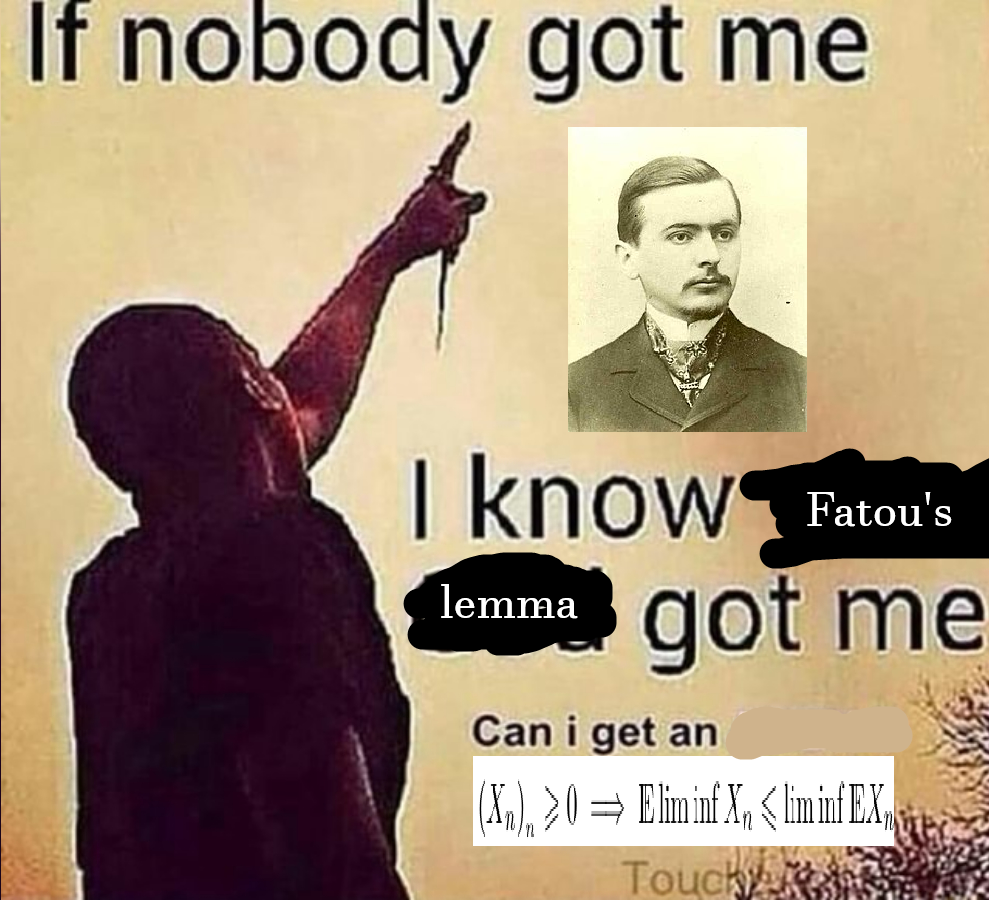
\includegraphics[width=0.6\linewidth]{fatou}
	\caption{The name Fatou is hard as fuck, if you ask me. Apparently he teamed up with a dude with no nose, look it up.}
	\label{fig:fatou}
\end{figure}
Remember that these results hold only almost surely, not up to equivalence!
\begin{theorem}
	Let $\F,\G$ be two sub-\sa{}s of $\HS$. Let $W$ and $X$ be $\HS$-measurable \rv{}s such that $\ev X,\ev WX$ exist. Then
	\begin{enumerate}[a)]
		\item $W\in\F\implies\ev_\F WX=W\ev_\F X$. This is called \emph{conditional determinism}: we can basically treat $W$ as a constant!
		\item $\F \subset\G\implies\ev_\F\ev_\G X=\ev_\G\ev_\F X=\ev_\F X$. So the smaller \sa{} ``wins'' over the larger: this is called \emph{repeated conditioning}.
	\end{enumerate}
\end{theorem}
\begin{fancyproof}
	\begin{enumerate}[a)]
		\item Let $X\in\HS_+,W\in\F_+$. Then we already know that $\xbar=\ev_\F\in\F_+$. Consider now
		\begin{equation*}
			\ev V(WX)=\ev\underbracket[0.6pt]{(VW)}_{\in\F_+}X\underbracket[0.6pt]{=\ev(VW)\xbar}_{\text{by projection property}}=\ev V(W\xbar)\quad\every V\in\F_+
		\end{equation*}
		and hence $W\xbar=W\ev_\F X$ is a version of $\ev_\F(WX)$.
		\item Let $\F\subset\G,X\in\HS_+$. By definition we know that $E=\ev_\F X\in\F_+$ so $W\in\G_+$. But due to conditional determinism we have that $\ev_\G W=W$. Hence
		\[\ev_\G\ev_\F X=\ev_\F X.\]
		Now we have to prove that 
		\[\ev_\F\ev_\G X=\ev_\F X.\]
		Call $\ev_\G X=Y$ and $\ev_\F X=\xbar$, i.e.
		\[\ev_\F Y=\xbar.\]
		Clearly $\xbar\in\F_+$ (\checkmark measurability) and we still have to prove projection property. By the definition of $\xbar$ (as a version of $\ev_\F X$) we have that 
		\[\ev V\xbar=\ev VX\qquad\every V\in\F_+.\]
		Recall that $Y=\ev_\G X\in\G_+$ and nodice that $V$ is also $\G$-measurable since $V\in\F_+\subset\G_+$.
		For $Y$ we have that $\ev VY=\ev VX$ for every $V\in\G_+$ and especially for those that are also $\F_+$-measurable. Hence
		\[\ev V\xbar=\ev VY\]
		that is to say $\xbar$ is also a version of the conditional epectation $\ev_\F Y=\ev_f\left[\ev_\G X\right].$
	\end{enumerate}
\end{fancyproof}
\subsection{Conditioning as projection}
\begin{notation}
	Consider the space $L^{2}$. If we are talking about $\HS$-measurable functions that belong to $L^{2}$ we write 
	\[L^{2}(\HS)\ni X\]
	And if we have a sub-\sa{} $\F$ of $\HS$ we will know that $L^{2}(\F)\subset L^{2}(\HS)$.
\end{notation}
\begin{theorem}
	$\every X\in L^{2}(\HS)$ there exists a unique (up to equivalence) $\xbar\in L^{2}(\HS)$ such that 
	\[\ev|X-\xbar|^{2}=\inf_{\mathclap{Y\in L^{2}(\F)}}\ev|X-Y|^{2}.\]
	Furthermore, $	X-\xbar$ is orthogonal to $L^{2}(\F)$, i.e.
	\begin{equation*}
		\ev V(X-\xbar)=0\qquad\every V\in L^{2}(\F)
	\end{equation*}
\end{theorem}
Note that $L^{2}(\HS)$ is a complete Hilbert space in which the inner product of $X$ and $Y$ is given by $\ev XY$.
$\xbar$ is the \emph{orthogonal projection of the vector $X$} onto the subspace $L^{2}(\F)$ and the decomposition 
\[X=\xbar+\xtilde\]
holds.
\begin{fancyproof}
	Let's write the $L^{2}$-norm of $X$ calling it $\norm{X}$:
	\begin{equation*}
		\norm{X}=\norm{X}_{2}=\sqrt{\ev X^{2}}.
	\end{equation*}
	Fix $X\in L^{2}(\HS)$. Define 
	\begin{equation*}
		\delta=\inf_{\mathclap{Y\in L^{2}(\F)}}\norm{X-Y}.
	\end{equation*}
	Let ${(Y_{n})}_{n}\subset L^{2}(\F)$ such that $\delta_n=\norm{X-Y_{n}}\xrightarrow[x\to\infty]{}0$. Let us prove that ${(Y_{n})}_{n}$ is a Cauchy sequence for the $L^{2}(\F)$-convergence.
	\begin{equation*}
		|Y_n-Y_m|^{2}=2|X-Y_{m}|^{2}-4|x-\underbracket[0.6pt]{\frac{1}{2}(Y_{n}+Y_{m})}_{\in L^{2}(\F)}|^{2}.
	\end{equation*}
	Take the expectation on both sides:
	\begin{equation*}
		\ev	|Y_n-Y_m|^{2}\leq2\delta^{2}_{m}+2\delta_n^{2}-4\delta^{2}.
	\end{equation*}
	Now we take the limit for $n$ and $m$ and what we get is
	\[\lim_{m,n\to\infty}\ev|Y_{n}-Y_{m}|^{2}\leq 0.\]
	Hence it is true that ${(Y_{n})}_{n}$ is Cauchy and this means that there exists a $\xbar\in L^{2}(\F)$ such that $\norm{Y_{n}-\xbar}\xrightarrow[n\to\infty]{}0$. Note that $\xbar$ is unique up to equivalence (by definition of $L^{2}$-norm). Note also
	\begin{equation*}
		\xbar\in L^{2}(\F)\implies \norm{X-\xbar}\geq \delta.
	\end{equation*}
	Now, by Minkowski's inequality we can write that
	\begin{equation*}
		\norm{X-\xbar}\leq\norm{X-Y_{n}}+\norm{Y_n-\xbar}\xrightarrow[n\to\infty]{}\delta+0=\delta.
	\end{equation*}
	We have thus 
	\begin{equation*}
		\norm{X-\xbar}=\delta.
	\end{equation*}
	For $V\in L^{2}(\F)$ and $a\in\R$, since $\ev|X-\xbar|^{2}=\delta$ then we have that
	\begin{align*}
		a^{2}\ev V^{2}-2a\ev V(X-\xbar)+\delta^{2}&=\norm{aV-(X-\xbar)}^{2}\\
		&=|\negthinspace|X-(\underbrace{aV+\xbar}_{\in L^{2}(\F)})|\negthinspace|^{2}=\delta^{2}
	\end{align*}
	And therefore 
	\begin{equation*}
		a^{2}\ev V^{2}-2a\ev V(X-\xbar)\leq 0\qquad\every a\in\R
	\end{equation*} which is impossible unless
	\[\ev V(X-\xbar)=0.\]
\end{fancyproof}
\subsection{Conditional expectations given \rv s}
Consider $Y$, a \rv{} on a measurable space. We have $\sigma Y$ that denotes the \sa{} generated by $Y$. But $\sigma Y$ is also the set of numerical \rv s of the form $f\circ Y$ for a deterministic function $f$. 
\begin{definition}
	The conditional expectation of $X$ given $Y$ is
\[\ev_{\sigma Y} X\]
If ${(Y_{t})}_{t\in T}$ is a collection of \rv s taking values in some measurable space. the conditional expectation of $X$ given ${(Y_{t})}_{t\in T}$ is
\[\ev_\F X,\;\text{ where }\F=\sigma\left({(Y_{t})}_{t\in T}\right).\]
\end{definition}
\begin{theorem}
	Let $X\in\HS_+$. Let $Y$ be a \rv{} taking values in the measurable space $(E,\E)$. Then every version of $\ev_{\sigma Y} X$ has the form $f\circ Y$ for some $f\in\E_+$.\\
	Conversely, $f\circ Y$ is a version of $\ev_{\sigma Y}X$ \ifonly{} 
	\[\ev f\circ Y\cdot h\circ Y=\ev X\cdot h\circ Y\qquad\every h\in\E_+.\]
\end{theorem}
Actually the last equality is just the projection property, if we think about it hard enough. The notation is once more problematic, though.
\begin{notation}
	\cinlar has a specific notation for conditional expectation, which is $\ev_{\sigma Y}X$. He is stupid and autistic because the whole world uses $\ev(X|Y)$. Professor Polito says that ``Oh well but $\ev_{\sigma Y}X$ is more precise b-because it's more rigorous'' well SHUT UP. SHUT UP NO ONE USES IT NO ONE EVEN KNOWS WHAT A FUCKING $\sigma$-ALGEBRA EVEN IS AND YOU KNOW WHY? BECAUSE IT IS USELESS BECAUSE ALL OF THIS SHIT IS USELESS IT IS A WASTE OF TIME AND IT IS NOT EVEN REMOTELY INTERESTING. LIKE I HAVE A FRIEND WHO STUDIES GEOLOGY THEY \textit{LITERALLY STUDY FUCKING ROCKS} THEY STUDY ALL THE MINUTE CHEMICALS ON THE ROCKS YOU FIND ON THE GROUND THEY STUDY HOW MANY FUCKING DINOSAURS SHITTED AND PISSED AND CUMMED ON THAT FUCKING ROCK AFTER IT GOT EJECTED BY A STUPID VOLCANO A MILLION YEARS AGO AND IT IS MORE INTERESTING AND USEFUL THAN THIS LIKE IT IS LITERALLY MORE USEFUL KNOWLEDGE IN ANY REAL DATA SCIENCE JOB WHERE ANYONE LITERALLY SAYS $\ev(X|Y)$ BECAUSE THAT'S WHAT YOU NEED TO KNOW YOU ONLY NEED TO KNOW THAT WE KNOW THAT $Y$ HAPPENED WHEN WE EVALUATE THE PROBABILITY OF $X$ YOU DON'T NEED TO KNOW ANYTHING ELSE I DON'T CARE AND NO ONE CARES.\\
	
	\vspace{0.05cm}The two notations are interchangeable but $\ev_{\sigma Y}X$ is preferrable.
\end{notation}
\subsection{Conditional probabilities and distributions}
\begin{definition}
	For every event $H\in\HS$
	\[\pr_\F(H)=\ev_\F\indi_H\]
	is called \emph{conditional probability of $H$ given $\F$} (with $\F$ beinf a sub-\sa{} of $\HS$).
\end{definition}
Lol what the fuck? Why are we defining probability through expectation? I don't know but remember that conditional expectation is a full-fledged \rv{}!
\begin{definition}
	Consider two events, $G$ and $H$. The conditional probability of $H$ given $G$ is the number $\pr_G(H)\in[0,1]$ satisfying
	\[\pr(G\cup H)=\pr(G)\pr_{G}(H)\]
	that is unique if $\pr(G)>0$.
\end{definition}
So in this case is not a \rv{} anymore but only a number.\\
Let us consider the conditional probability $\pr_\F H\every H\in\HS$ (we will remove parentheses from now on because you suck and you should die). Let $Q(H)$ be a version of $\pr_\F H$ (remember... conditional probabilities are now expectations!). Assume $Q(\emptyset)=0$ and $Q(\Omega)=1$.\par
$Q(H)$ is a \rv{} and it is $\F$-measurable by definition. Let $Q_\omega(H)$ be the value at point $\omega\in\Omega$. 
\begin{notation}
	If we called $Q(H)=Z$ then $Q_\omega(H)$ would be $Z(\omega)$.
\end{notation}
So what is $Q$ actually? It is a function $Q:(\omega, H)\mapsto Q_\omega(H)$ whith $\omega\in(\Omega,\F)$ (a subset of $(\Omega, \HS)$) and $H\in(\Omega,\HS)$. This is similar to a transition kernel... A transition kernel from $(\Omega,\F)$ into $(\Omega,\HS)$. But it is really? Do we care? Of course not, but we need to check because we need more reasons to end our life by our hand.
	For something to be a transition kernel it should verify:
	\begin{enumerate}
		\item the mapping $\omega\mapsto Q_\omega(H)$ should be $\F$-measurable (in this case it is ok for every $H\in\HS$\checkmark);
		\item for every disjoint sequence ${(H_n)}_{n}\in\HS$ it should hold $\every\omega\in\Omega$ the following:
		\begin{equation}
			Q_\omega\left(\bigcup_n H_n\right)=\sum_n Q_\omega(H_{n})\tag{$\star$}\label{asfucked}.
		\end{equation}
	\end{enumerate}
This last requirement arises a problem: we could apply monotone convergence theorem for conditional expectations, but we know that those property hold only almost surely! I can already hear the reader say ``oh but why should we care isn't it supposed to be like the same of saying ``equal to'' and things like this and so on'' but well, my dear idiotic little shit, when something is almost surely it is actually \textit{almost} surely. It means that you're \textit{almost} guaranteed that nothing will fuck you in the ass unless something is small enough to creep in your asshole without you even noticing. Thank measure theory enthusiasts for this.
\begin{figure}[H]
	\centering
	
\includegraphics[width=0.6\linewidth]{asnkae2}
	\caption{Snake has had enough and honestly so do I.}
	\label{fig:asnkae2}
\end{figure}
The fact is that we could have some $\omega$'s with measure zero so technically there are some exception points for which it doesn't hold. These points depends on the choice of the sequence $H_n$. Let $\Omega_0$ be the set for which (\ref{asfucked}) holds:
\[\Omega_0=\bigcap_h\Omega_h\]
where $\Omega_h$ is the almost surely  set including all $\omega$ for the sequence $h={(H_n)}_{n}$. But we may have uncountably many problems... Why are there so many problems with conditional expectation? The root of the problem is that conditional expectation is not an exactly well-defined object.
\begin{definition}
	Let $Q(H)$ be a version of $\pr_\F(H),\every H\in\HS$. Then $Q:(\omega,H)\mapsto Q_\omega(H)$ is said to be a \emph{regular version} of the conditional probability $\pr_\F$ provided that $Q$ is a transition probability kernel from $(\Omega,\F)$ into $(\Omega, \HS)$.
\end{definition} 
\begin{proposition}
	Let $\pr_\F$ have a regular version $Q$. Then
	\begin{equation*}
		QX:\omega\mapsto Q_\omega X=\int_\Omega Q_\omega(\dw')X(\omega')
	\end{equation*}
	is a version of $\ev_\F X\every \text{\rv{} }X$ whose expectation exists.
\end{proposition}
So we are integrating over $\Omega$ our function $X$ against our regualar version of the conditional probability $Q$.
\begin{theorem}
	If $(\Omega,\HS)$ is a standard measurable space (which means that it is isomorphic to $(F,\B_F)$ for some Borel subset $F$ of $\R$). Then $\pr_\F$ has a regular version.
\end{theorem}
So as long as we work in standard measurable spaces we do not need to worry. Now that we have assessed this fact we can define the concept of conditional distribution.
\begin{definition}
	Consider a \rv{} $Y$ taking values on $(E,\E)$ and a sub-\sa{} $\F$ of $\HS$. The \emph{conditional distribution of $Y$ given $\F$} is any transition probability kernel
	\begin{equation*}
		L:(\omega,B)\mapsto L_{\omega}(B)
	\end{equation*}
	From $(\Omega,\F)$ into $(E,\E)$ such that
	\begin{equation*}
		\pr_\F(Y\in B)=L(B),\qquad B\in\E.
	\end{equation*}
 \end{definition}
 Here we already have our probability distribution of $Y$ with our probability meaure that $Y$ belongs to $B$ for every $B\in\E$. So the conditional transition is a transition probability kernel and moreover, if $\pr_\F$ has a regular version $Q$ then 
 \begin{equation*}
 	L_\omega (B)=Q_\omega (\{Y\in B\}),\qquad\omega\in\Omega,B\in\E
 \end{equation*}
 Defines a version $L$ of the conditional distribution of $Y$ given $\F.$
 \begin{notation}
 	This would be 
 	\[\pr(Y\in B|\F).\]
 \end{notation}
 \begin{theorem}
 	If $(E,\E)$ is a standard measurable space then there exists a version of the conditional distribution of $Y$ given $\F$.
 \end{theorem}
 We will use this notion to perform a reverse operation that we did several lectures ago when we built measures on product spaces. Back then we talked about kernels in which the dependence structure is actually included in the kernel measure in itself.
 \subsection{Disintegration of measures}
 There may be a The Cure joke but my spirit is already too beaten down to think about one. We introduced measures on product spaces using $\Sigma$-finite transition kernels from $(D,\D)\to(E,\E)$:
 \begin{equation}
 	\pi f=\int_D\mu(\dx)\int_E K(x,\dy)\underbracket[0.6pt]{f(x,y)}_{\mathclap{\in\left(\D\otimes\E\right)_{+}}}\tag{$\circ$}\label{disintegrate}.
\end{equation}
 This integral defines a measure $\pi$ on $(D\times E,\D\otimes\E)$. This measure $\pi$ is $\sigma$-finite and unique if $\mu$ is $\sigma$-finite and $K$ is $\sigma$-bounded.\\
 Let $(D,\D)$ and $(E,\E)$ be measurable spaces and let $\mu$ be a probability measure on $(D,\D)$. Let $K$ be a probability transition kernel from $(D,\D)$ into $(E,\E)$. Consider the measure $\pi$ on the product space:
 \begin{equation*}
 	\pi f=\int_{D\times E}f(x,y)\pi(\dx,\dy).
 \end{equation*}
 Note also that $\pi$ is the unique measure satisfying 
 \begin{equation*}
 	\pi(A\times B)=\int_A\mu(\dx)K(x,B),\qquad\text{ with }\begin{array}{l}
 		A\in\D\\
 		B\in\E\\
 		x\in D\\
 		y\in E.
 	\end{array}
 \end{equation*}
 We can also write the same thing in differential notation as
 \begin{equation*}
 	\underbracket{\pi(\dx\dy)}_{\text{joint distr.}}=\underbracket{\mu(\dx)}_{\text{distr. of }X}\underbracket{K(x,\dy)}_{\text{\parbox{10em}{conditional probability that $Y\in\dy$ given that $X=x$}}}.
 \end{equation*}
 \begin{theorem}
Let $\pi$ be a probability measure on $(D\times E,\D\otimes\E)$. Let $(E,\E)$ be a standard space. Then there exists a probability measure $\mu$ on $(D,\D)$ and a transition probability kernel $K$ from $(D,\D)$ into $(E,\E)$ such that (\ref{disintegrate}) holds.
\end{theorem}
\begin{fancyproof}
	Let $W=D\times E,\mathscr{W}=\D\otimes\E,\pr=\pi$ so that we have our probability space $(W,\mathscr{W},\pi)$. Now on this space we can define the \rv s $X$ and $Y$. Consider the notation $w\in W$: $w$ has two components so that $w=(x,y)$. Define
	\begin{align*}
		X &\text{ s.t. }X(w)=x\text{ (it gives us the first coordinate)}\\
		Y &\text{ s.t. }Y(w)=y\text{ (it gives us the second coordinate)}.
	\end{align*}
	Further, let $\mu$ be the distribution of $X$, that is $\mu(A)=\pi(A\times E),\;A\in\D$.
	Also note that $Y$ takes values in $(E,\E)$ which is standard. Since $(E,\E)$ is standard it exists a regular version that we can call $L$ of the conditional distribution of $Y$ given the sub-\sa{} $\F=\sigma X$. So this \rv{} is measurable with respect to $\F$ that in this case is $\sigma X$. But we know that if a \rv{} is measurable with respect to the \sa{} generated by another \rv{} then we know that the first \rv{} is just a deterministic function of the second \rv{} (in this case $X$). Hence $L$ is a function of $X$ and
	\begin{equation*}
		L_w(B)=K(X(w,B)\qquad\text{(it doesn't depend on $Y$ at all!)}
	\end{equation*}
	where $K$ is a transition kernel from $(D,\D)$ into $(E,\E)$. By the projection property for $L$ we have:
	\begin{align*}
		\pi(A\times B)&=\ev\indi_A\circ X\cdot\indi_B\circ Y=\ev\indi_A\circ X\cdot K(X,B)\\
		&=\int_D \indi_A\mu(\dx)K(x,B).
		\end{align*}
		So for indicators (\ref{disintegrate}) holds.
\end{fancyproof}
Once we proved this for indicators we can go on for simple functions and positive functions in the usual way.
\begin{theorem}
	If $H$ has the representation (\ref{disintegrate}) then the kernel $L$
	\begin{equation*}
		L_w(B)=K(X(w),B)\qquad w\in\N,B\in\E
	\end{equation*}
	is a \emph{version of the conditional distribution} of $Y$ given $\F$.
\end{theorem}
\subsection{Conditional independence}
We are now going to relate what we have studied so far with the idea of conditional probability. \\
\begin{definition}
	Consider some sub-\sa s of $\HS$:
\[\F,\F_1,\F_2,\ldots,\F_n\]
Then the sub-\sa{}s $F_1,\F_2,\ldots,\F_n$ are said to be \emph{conditionally independent given $\F$} if
\begin{equation*}
	\ev_\F V_1\cdot V_2\cdot\ldots\cdot V_n=\ev_\F V_1\cdot\ev_\F V_2\cdot\ldots\cdot\ev_\F V_n
\end{equation*}
for every positive \rv s $V_1,V_2,\ldots,V_n$ measurbale with respect to $\F_1,\F_2,\ldots,\F_n$ resepctively.
\end{definition}
Note that the usual notion of independence corresponds to the specific choice of trivial \sa:
\begin{equation*}
	\F=\left\{\emptyset,\Omega\right\}.
\end{equation*}
It is over. It is finally over and I am a considerably worse persone now. Martingales, anyway, are very linked to the notion of conditional probability... And so a lot of other stochastic processes. Whatever.

\chapter{A first study in stochastic processes: Martingales}
Okay, I'll admit that this part is really hard for me to follow. I am already broken down by Professor Polito's lectures and right now... I only want to be happy again. Please note that the astonishing drop in the quality of the notes is not my fault. This shit should be easier to explain but they manage to mess this up anyway. 
\section{Revising stochastic processes and filtrations}
\begin{notation}
	\begin{enumerate}
		\item we will work in a fixed probability space $(\Omega,\HS,\pr)$;
		\item we will denote an index set $\T$ (which is usually interpreted as time). It could be $\T=\N$ or $\T=\R$, for example;
		\item $\{X_t:t\in \T\}$ is a \rv{} taking values in the product space
		\[(F,\F)=(E^{\T},\E^\T).\]
		We can think of this as an evolving stochastic process.
	\end{enumerate}
\end{notation}
Let $\T$ be a subset of $\R$. For each $t\in\T$ let $\F_t$ be a sub-\sa{} of $\HS$. The family $\F=\left\{\F_t:t\in\T\right\}$ is called a \emph{filtration} provided that
\[\F_s\in\F_t\qquad\every s<t.\]
\begin{definition}
	A \emph{stochastic process} $X={(X_t)}_{t\in\T}$ generates a filtration that is named \emph{natural filtration}.
\end{definition}
As the time passes, I discover more and more information about $\HS$. Each process defines a filtration by generating a ``flow of information''.
\begin{example}
	Imagine a car competition composed by two different races. Consider the events
	\[\begin{array}{l}
		\omega=\left\{\text{car $A$ wins}\right\}\\
		\ell=\left\{\text{car $A$ loses}\right\}.
	\end{array}\]
	Consider 2 races: our $\Omega$ will be
	\[\Omega=\left\{\omega\omega,\ell\omega,\omega\ell,\ell\ell\right\}.\]
	Before the starting of the race, at time 0, we have no information about what is going to happen so our filtration will be
	\[\F_0=\left\{\underbracket{\left\{0\right\}}_{\emptyset},\underbracket{\left\{\omega\omega,\ell\omega,\omega\ell,\ell\ell\right\}}_{\Omega}\right\}\]
	which is the trivial \sa{}. Remember that in this case the empty set $\emptyset$ represents impossible events (e.g. all cars win all races). So the \rv{} $X_0$ measurable with respect to $\F_0$ maps all the outcomes of the race to the same value. The idea is that we cannot ask ourselves ``what is the probability of the car winning the first and the second race?'' because we aren't able to measure these events in $\HS$. Now consider the situation after the first race: I am now able to ``discern'' the events regarding the first race:
	\[\F_1=\left\{\left\{0\right\},\left\{\omega\ell,\omega\omega\right\},\left\{\ell\ell,\ell\omega\right\},\left\{\omega\omega,\omega\ell,\ell\omega,\ell\ell\right\}\right\}.\]
	Now I am able to know what happened after the first race and this gives me a richer sub-\sa, with $\F_0\subset{\F_1}$. I am now able to have a \rv{} $X_1$ that is measurable with respect to $\F_1$. For instance, imagine defining the following \rv:
	\[X_1=\begin{cases}
		1 &\text{if the car wins the first race}\\
		0 &\text{otherwise}.
	\end{cases}\]
	But, for instance, the \rv{} ``the car wins the second race'' is still not measurable with respect to $\F_1$. Consider now the filtration after the second race:
	\[\F_1=\left\{\left\{0\right\},\{\omega\omega\},\{\ell\ell\},\{\omega\ell\},\{\ell\omega\},\left\{\omega\ell,\omega\omega\right\},\left\{\ell\ell,\ell\omega\right\},\left\{\omega\omega,\omega\ell,\ell\omega,\ell\ell\right\}\right\}.\]
	Of course $\F_2\supset\F_1\supset\F_0$. We could define a \rv{} $X_3$ of the following type:
	\[X_3=\begin{cases}
		0 \\
		1\\
		2\\
	\end{cases}\]
	which counts the numbers of victories of our car. $X_3$ is $\F_2$-measurable but not $\F_1$-measurable.
	Now $\F$ is a filtration:
	\[\F=\left\{\F_0,\F_1,\F_2\right\}.\]
\end{example}
\begin{example}
	What if the same experiment is observed by different people? In other ways, what if we have different learning from the same experiment? Imagine that we have two filtrations $\F$ and $\G$. We say that $\F$ is finer than $\G$ if
	\[\F_t\supset\G_t\qquad\every t\in\T.\]
\end{example}
\begin{definition}
	Given $\F={(\F_t)}_{t\in\T}$, a stochastic process ${\{X_t\}}_{t\in\T}$ is \emph{adapted} to $\F$ if $X_{t}$ is $\F_t$-neasurable for each $t\in\T$ and $\E$-measurable.
\end{definition}
We already mentioned that every process generates its \textit{natural filtration} $\sigma(X_{t},t\in\T)$, for which the process is clearly adapted. But we may want to consider another filtration $\F=(F_t)$ such that $\{X_t\}$ is adapted to $\F$ because all the information on $X$ that I care about are contained in this filtration. What does this mean and what  is the relationship between the two? Which one of the two is finer considering that our process is adapted to both? The answer is 
\[\F\supset\sigma(X_t)\qquad\text{($\F$ is finer than the natural filtration)}\]
because $\sigma(X_t)$ is always the smallest possible \sa{} that a process can generate (the natural filtration is the \textit{minimum} filtration). \\
Another way we could see the question of adaptation is:
\begin{center}
	``Can $X$ be determined using only information available in $\F$?''
\end{center}
If yes, then $X$ is adapted to $\F$.
\begin{example}
	This is called ``the secretary problem'': in this case we must start from the filtration and then understand the problem.
	Here i have $N$ candidates for a position; a candidate disregarded after the interview is lost. The interviewer wants to hire exactly 1 candidate and each candidate has different abilities and the interviewer knows only the relative ability of those already interviewed so far. Our goal is to maximizing the probability of hiring the best one. We have three questions:
	\begin{enumerate}
		\item what is $\Omega$?
		\item what is the filtration $\F$ for this experiment?
		\item what process should we use?
	\end{enumerate}
	In this case $\Omega=N!$ permutations of the ranking of the candidates (the order in which they show up) and the filtration is the information earned from interview up to time $t$ (that is the ranking of the candidates up to time $t$). But what is the process that I should use? Consider the sequence
	\[V_1,V_2,\ldots\qquad{\{V_i\}}_{i\geq 1}\]
	with $V_i=1$ if and only if the best candidate is the $i$-th candidate and $V_i=0$ otherwise. Could this process ${\{V_i\}}_{i\geq 1}$ be used? No, because $V$ is not adapted to $\F$... because to understand if $i$-th candidate is te best we need to compare it to the other candidates, including the ones that didn't show up yet! But then how can we get an adapted process? Let us consider the expectation
	\[U_n=\ev\left[V_n|\F_n\right]\]
	What do we know about the measurability of $U_n$? We know that it is for sure $\F_n$-measurable. This trick gives us a simple way to build an adapted process. So now we will have:
	$U_n=
		0$ if the candidate is not the best up to $n$ and $U_n=1$ otherwise. More specifically, we will have
		\begin{align*}
			U_n&=1\cdot\substack{\text{proability that the best candidate}\\\text{is among the first $n$}}+0\cdot\substack{\text{proability that the best candidate}\\\text{is not among the first $n$}}\\
			&=1\cdot\frac{n}{N}+0\cdot\frac{N-n}{N}.\\
			&=\frac{n}{N}
		\end{align*}
	This is a quantity that I can measure and it is therefore adapted.\par
\end{example}
\begin{figure}[h]
	\centering
	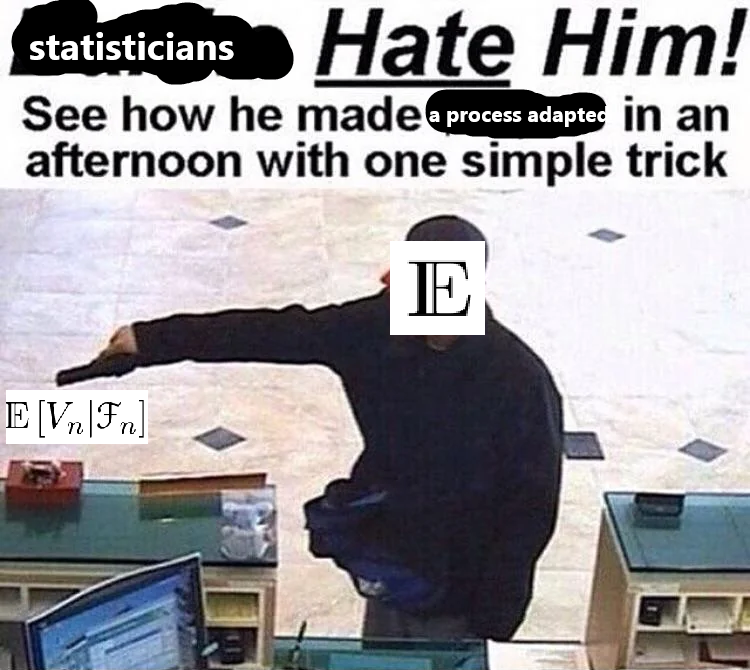
\includegraphics[width=0.7\linewidth]{screenshot009}
	\caption{You conditioned in the wrong hood, buddy.}
	\label{fig:screenshot009}
\end{figure}
\subsection{Stopping times}
Consider now the same problem under a different point of view: we want to establish the ``best time'' when to stop discarding candidates. This is a random time and it is called a \emph{stopping time}. This is nothing else than a time that we choose basing ourselves on elements or events that may or may not happen: this is why they're a \rv. The stopping times are a random variable that can cause problems, since stopping times can be infinite: imagine that our stopping time is "whenever a volcano erupts" but the stupid fucking volcano decides to go into quiescence forever. This is why beside our index set $\T$ we need to introduce $\Tbar=\T\cup\{\infty\}$.
\begin{definition}
	\[T:\Omega\mapsto\Tbar
	\]
	is called \emph{stopping time} of $\F$ if
	\[\{T\leq t\}\in\F_t\qquad\every t\in\T.\]
\end{definition}
Remember that stopping times have to be $\F$-measurable: for example "when will the fucking volcano erupt for the last time" is \textit{not} a stopping time because it requires information that we don't have in $t$! \\
Stopping time have an alternative definition:
\begin{definition}
	$T$ is a stopping time if the process
	\[Z_t=\indi_{\{T\leq t\}}\qquad t\in\T\]
	is adapted to $F$.
\end{definition}
From this definition it follows that when $\T=\N$ then this is equivalent to having
\[\underbracket[0.6pt]{\hat{Z}_{n}}_{\mathclap{Z_n-Z_{n-1}}}=\indi_{\{T=1\}}\qquad\every n\in\N\]
that needs being adapted to $\F_n$.\\
Not all random times are stopping time: think about an experiment in which we produce a signal when a physical event happens. Let us call $Z$ the process indicator and $T$ our stopping time:
\[Z_t{\omega}=\begin{cases}
	0&t<T(\omega)\\
	1&t\geq T(\omega).
\end{cases}\]
Then if the information flow allows us to recognize the occurrence of the event then $T$ is a stopping time.
\begin{example}
	Some stopping times:
	\begin{enumerate}[\circnum]
		\item The first time that $X(\omega)\in H\in\Omega$;
		\[T(\omega)=\begin{cases}
			\inf \left\{n\in\N:X_n(\omega)\in H\right\}&\\
			+\infty&\text{if $X_n(\omega)\notin H\;\every n$}
		\end{cases}\]
		So
		\[\left\{T\leq n\right\}=\bigcup_{k=0}^{n}\left\{X_k\in H\right\}.\]
		\item Consider i.i.d. \rv{}s 
		$X_1,X_2,\ldots$. Consider the probabilities
		\[\pr(X_i=1)=\pr(X_i=-1)=\frac{1}{2}\]
		and the random walk
		\[S_n=\sum_{1}^{n}X_i.\]
		Let's define 
		\[T_1=\begin{cases}
			\min\left\{n<50:S_n=3\right\}\\
			50 &\text{otherwise}.
		\end{cases}\]
		This is a stopping time because I can write $\left\{T_1\leq n\right\}$ as $$\underbracket[0.6pt]{\bigcup_{k=1}^{n}\underbracket[0.6pt]{\left\{S_k=3\right\}}_{\text{$\F_k$-measurable}}}_{\mathclap{\text{$\F_n$-measurbale}}}\qquad n<50.$$
		Moreover for $n=50$ we have $T_{1}\in\F_{50}$.
		\item Starting from the previously deifned random walk, consider the quantity 
		\[M_n=\min(S_1,\ldots,S_n)\]
		And the random time
		\[T_2=\min\left\{n:S_n\geq M_m+2\right\}\]
		is a stoppimg time. On the contrary, 
		\[T_3=\begin{cases}
			\max\left\{n<50:S_n=7\right\}&\text{if not empty}\\
			50 &\text{otherwise}
		\end{cases}\]
		is not a stopping time. Why? Because I have to wait until $n=50$ to answer the question. 
	\end{enumerate}
\end{example}

Consider the random times on $\R_+$
\[0<T_1<T_2<\ldots\]
With $\lim_{n\to\infty}T_n=+\infty$. Define the process $\left\{N_t\right\}$ as 
\[N_t:=\sum\indi_{[0,t]}(T_n).\]
This is called \emph{counting process}. It is a basic count of the number of events happened up to time $n$.
\begin{figure}[H]
	\centering
	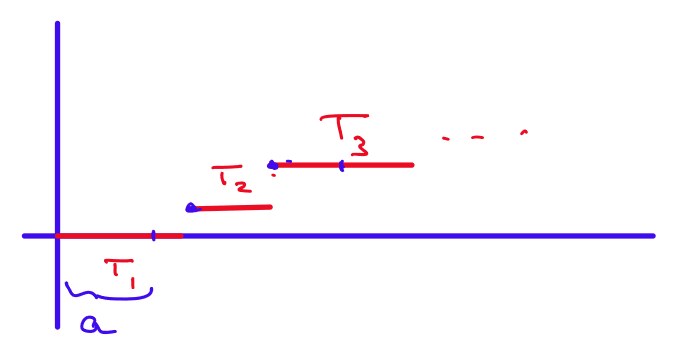
\includegraphics[width=0.6\linewidth]{screenshot010}
	\caption{Yeah I'm counting on ending my life very soon.}
	\label{fig:screenshot010}
\end{figure}
$N_{t}$ is increasing, right continuous and incresases by unitary jumps. Moreover, $N_0=0$, $N_t<\infty$ for $t\in\R_+$. Of course $\lim_{t\to\infty}N_t=\infty$. Counting processes generate their natural filtration $\F$.

Some problems require to stop the observation at a stopping time (because we don't care anymore\footnote{Assuming we ever did.})... So we don't actually need the whole knowledge of the complete filtration $\F={\left(\F_t\right)}_{t\geq 0}$. The problem is that as we said before the stopping time is a random time. So what we need is the \textit{information known up to time $T$} $\F_T$, basically the $\sigma$-field that is the filtration at time $T$. 
\begin{remark}
	We said that $\F_t$ does not include $t=\infty$... but $T$ may diverge to $\infty$! We need to enlarge $\F$ to include $t=\infty$.
\end{remark}
Think, for instance the stopping time ``first time of overflowing of a dam''. It is something that may very well never happen and is therefore called ``Vajont stopping time\footnote{Okay I'm sorry I'm sorry I am a terrible person yes sir yes yes I concur it was an extremely inappropriate joke yes yes sir yes you have my word yes no no never again no you don't have to worry no no.}''.
\begin{definition}
	Let $\Tbar=\T\cup\left\{+\infty\right\}$. We define
	\[\F_\infty=\lim_{t\to\infty}\F_t=\underbracket{\bigvee_{t\in\T}\F_+}_{\sigma\left(\bigcup\F_t\right)}.\]
\end{definition}
\begin{definition}
	$\F_{\Tbar}$ is a filtration on $\Tbar$ and $T$ is a stopping time on it if and only if it is a stopping time on $\F_\T$.
\end{definition}
\begin{remark}
	Every stochastic process on ${(\F_{t})}_{t\in\T}$ can be extended to $\Tbar$ by appending any \rv{} $X_\infty$ to it (with $X_\infty\in\F_{\infty}$).
\end{remark}
So adding this \rv{} doesn't really add any information but only ensures that nerds don't whine about completeness. It is \textit{technically} information that we will never user, since $\F_\infty$ does not contain any further information with respect to $\F$. We denote with $\F$ also the extended filtration, with the ease of mind given by the fact that a divergent stopping time won't make us commit harakiri.
\begin{definition}
	Let $\F$ be a filtration on $\Tbar$ and let $T$ be a stopping time on $\F$. We call \emph{past until $T$} the \sa{} $\F_t\subset\F_\infty\subset\HS$ such that:
	\[\F_T=\left\{H\in\HS:H\cap\{T<t\}\in\F_t,\every t\in\Tbar\right\}.\]
\end{definition}
This means that $\F_T$, which represents the evolution within $T$, contains all the events $H$ such that they are before the stopping time in all the filtrations. This is selecting the events $H$ that happen within the time $T$.
\begin{remark}
	If we fix a $T\equiv t$ then $\F_T\equiv\F_t$ (it's the normal filtration at time $t$).
\end{remark}
If $T$ is a stopping time of $\F$ then $\{T\leq r\}$ belongs to $\F_T,\;\every r\geq 0$:
\[\{T\leq r\}\cap\{T\leq t\}=\{T\leq\min(T,r)\}\in\F_t\]
So $T$ is $\F_T$-measurable. 
\begin{remark}
	$\F_t$ can be read as the collection of all $\F_t$-measurable \rv{}s $V$: the value of $V(\omega)$ can be told by the time $T(\omega)$: we can read the value of $V(\omega)$ before the ringing of an alarm.
\end{remark}
\begin{theorem}
	A random variable $V$ belongs to $\F_T$ if and only if
	\begin{equation}
		V\indi_{T\leq t}\in\F_t,\qquad\every t\in\Tbar.\tag{$i$}\label{stopstopstop}
	\end{equation}
	If $\Tbar\equiv\overline{\N}$ the condition becomes
	\begin{equation*}
		V\indi_{T=n}\in\F_n\qquad\every n\in\overline{\N}.
	\end{equation*}
\end{theorem}
\begin{fancyproof}
	Note that 
	\[X_t=V\indi_{T\leq t}\]
	is a stochastic process. For $\every r\in\R_+$ and $t\in\T$
	\[\{V>r\}\cap\{T\leq t\}=\{X_t>r\}.\]
	But now we know that (\ref{stopstopstop}) is just a consequence of the definition of $\F_t$:
	\[\{V>r\}\in\F_T\quad\every r\underset{\text{def. of $\F_T$}}{\iff}\{X_t>r\}\in\F_t\qquad\every r,\every t\in\Tbar\]
	The special case in which $\Tbar\equiv\overline{\N}$ means that
	\[V\indi_{\{T=n\}}=\begin{cases}
		X_n-X_{n-1}&\text{if }n\in\N\\
		X_\infty-\sum_{n\in\N}(X_n-X_{n-1})&\text{if }n=\infty
	\end{cases}\]
	so that 
	\begin{equation*}
		V\in\F_T\iff V\indi_{T=n}\in\F_n
	\end{equation*}
\end{fancyproof}
But what if there is a problem that involves more than 1 stopping time? We cannot use two different ``pasts'' because that would cause problems with the measurability of \rv s. 
\begin{example}
Imagine a factory. The production is blocked when
\begin{enumerate}[a)]
	\item the temperature of the room is above a certain threshold; 
	\item the machinery has not been cleaned for more than 12 hours.
\end{enumerate}\par
Alternatively, imagine that the sales of shares happens:
\begin{enumerate}[a)]
	\item when the price is above a fixed value;
	\item when the increase of the price is smaller than a fixed value.
\end{enumerate}
\end{example}
Both of this cases require the use of 2 different stopping times $S$ and $T$. We may think to evaluate two typical functions of $S$ and $T$ of interest:
\begin{equation*}
	\underbrace{\min\{S,T\}}_{S\wedge T}\qquad	\underbrace{\max\{S,T\}}_{S\vee T}
\end{equation*}
\begin{example}
	\emph{Truncated stopping time}: let $T$ be a stopping time (for example, the time at which we sell certain shares) and that we want a finite horizon for this decision. In this case the quantity of interest is
	\begin{equation*}
		S=T\wedge n=\min\{T,n\}
	\end{equation*}
	where $n$ could be some sort of time horizon.\\
	Imagine that two cyclists participate to a race. Their children will have their snack when both the parents will arrive to the finish line. How long will the children wait for their snack?
	We can think about the following stopping times:
\[ 	\begin{array}{l l}
		T: & \text{time employed by the first cyclist}\\
	S: & \text{time employed by the second cyclist}\\
	U: &\max\{S,T\}.
		
	\end{array} \]
	The waiting time for the children will be $U$.
\end{example}
This is cool and all, but are we sure that $S\wedge T$ and $S\vee T$ are stopping times?
\begin{remark}
	Yes.
\end{remark}
Why?
\begin{remark}
	Fuck you.
\end{remark}
Aw hell nah. Now even the color boxes are against me. 
\begin{insult}
	You will NEVER pass this exam.
\end{insult}
Well this is not a surprise.
\begin{insult}
	Not if you keep jerking around.
\end{insult}
\begin{fancyproof}
	We know that $\{S\leq t\}$ and $\{T\leq t\}$ belong to $\F_t$ for every $t$, since they are stopping times. Consider now $\left\{\min\{(S,T)\leq t\}\right\}$ and $\left\{\max\{(S,T)\leq t\}\right\}$. We have
	\begin{equation*}
		\left\{\min\{(S,T)\leq t\}\right\}=\underbrace{\underbrace{\{S\leq t\}}_{\in\F_t}\cup\underbrace{\{T\leq t\}}_{\in\F_t}}_{\in\F_t}
	\end{equation*}
	and 
	\begin{equation*}
			\left\{\max\{(S,T)\leq t\}\right\}=\underbrace{\underbrace{\{S\leq t\}}_{\in\F_t}\cap\underbrace{\{T\leq t\}}_{\in\F_t}}_{\in\F_t}.
	\end{equation*}
\end{fancyproof}
There is a further theorem:
\begin{theorem}
	\begin{enumerate}[\circnum]
		\item if $S\leq T\implies\F_S\subset\F_T$;
		\item $\F_{\min\{S,T\}}=\F_S\cap\F_T$;
		\item if $V\in\F$, the following processes are in $\F_{\min\{S,T\}}$:
		\begin{equation*}
			\begin{array}{c c c}
				\color{SteelBlue4}(a)&\color{SteelBlue4}(b)&\color{SteelBlue4}(c)\\
				V\indi_{S\leq T},&V\indi_{S=T},&V\indi_{S< T}.
			\end{array}
		\end{equation*}
	\end{enumerate}
\end{theorem}
\begin{fancyproof}
	\begin{enumerate}
		\item Imagine $\{S\leq T\}$. Now consider the event $\{S\leq n\}$. Since $S$ happens before $T$ then we have that $\{T\leq n\}\subset\{S\leq n\}$. We know that if $A\in\F_S$ then
		\[A\cap\{T\leq n\}=A\cap\underbracket[0.6pt]{\{S\leq n\}}_{\in\F_n}\cap\underbracket[0.6pt]{\{T\leq n\}}_{\in\F_n}\]
		which means that $A\cap\{T\leq n\}\in\F_n$ and by definition of $\F_T$
 this correponds to saying
 \[\F_S\subset\F_T.\]
 \item \begin{enumerate}
 	\item Let us first prove that $\F_{\min\{S,T\}}\subset\F_{S}\cup\F_T$.
 	Note that $\min\{S,T\}$ is dominated by $\F_s$ and $\F_T$, which means that $\F_{\min\{S,T\}}$ is included both in $\F_S$ and $\F_T$. By point 1 we have
 	\[\F_{\min\{S,T\}}\subset\F_S\cap\F_T.\]
 	\item It remains to prove that $\F_{\min\{S,T\}}\supset\F_{S}\cup\F_T$. Let $H\in\F_S\cap\F_T$. This means that 
 	\begin{equation*}
 		H\cap\{S\leq T\}\in\F_{\min\{S,T\}}
 	\end{equation*}
 	by part the of this theorem, since $H\in\F_S$. But we also know that
 	\[H\cap\{T\leq S\}\in\F_{\min\{S,T\}}\]
 	by part 3 of this theorem since also $H\in\F$. But this means that
 	\begin{equation*}
 		H=\left\{H\cap\left\{S\leq T\right\}\right\}\cup\left\{H\cap\left\{S\leq T\right\}\right\}
 	\end{equation*}
 	belongs to $\F_{\min\{S,T\}}$ and so
 	\[\F_{\{S\cap T\}}\subset\F_{\min\{S,T\}}.\]
 \end{enumerate}
 \item\begin{enumerate}
 	\item $V\indi_{\{S\leq T\}}\in\F_{\min\{S,T\}}$. To prove this we use the following theorem:
 	\begin{theorem}
 		Let $T$ be a stopping time of $\F$. Then
 		\[\F_T=\{X_T:X\in\F\}\]
 		with $X$ in $\F$.
 	\end{theorem}
 	This baiscally means that $\F_t$ becomes the values $X_T$ of $X$ in $\F$ at time $T$. Let us consider $X_t=V\indi_{\{S\leq t\}}$ with $t=\min\{S,T\}$. We know that $\min\{S,T\}$ is a stopping time of $\F_{\min\{S,T\}}$ and by the theorem above
 	\[X_{\min\{S.T\}}\in\F_{\min\{S,T\}}\]
 	or, alternatively,
 	\[\indi_{\{S\leq T\}}\in\F_{\min\{S,T\}}.\]
 	\item Let $V=2\implies\{S\leq T\}\in\F_{\min\{S,T\}}$ and by symmetry $\{T\leq S\}\in\F_{\min\{S,T\}}$. This means that 
 	\begin{equation*}
 		\{S=T\}=\{S\leq T\}\cap\{T\leq S\}\in\F_{\min\{S,T\}}.
 	\end{equation*}
 	Furthermore 
 	\[\{S<T\}=\{S\leq T\}\setminus\{S=T\}\]
 	Which implies memebership of $\F_{\min\{S,T\}}$.
 	\item Consider the fact already proven that $V\indi_{\{S\leq T\}}\in\F_{\min\{S,T\}}$. Multiplying by $\indi_{\{S=T\}}$ or $\indi_{\{S<T\}}$ does not alter the membership in $\F_{\min\{S,T\}}$.
 \end{enumerate}
 	\end{enumerate}
\end{fancyproof}
Consider now a machinery what when it becomes too hot (above a certain threshold) an alarm rings and after 3 seconds the machinery stops. Here we deal with 2 times:
\begin{equation*}
	\begin{array}{l l}
		T: &\text{time of the alarm (stopping time)}\\
		t=3: &\text{deterministic time (stopping time as well)}\\
	\end{array} 
\end{equation*}
and the time of our interest is the time $S$ when the machinery stops:
$$S=T+t$$
\begin{remark}
	At time $T$ we know $S$: We know that when the alarm rings within three seconds the machinery will stop, so $S$ is actually $\F_T$-measurable. We say that \emph{$S$ is foretold by $T$}.
\end{remark}
\begin{definition}
	Let 
	\begin{equation*}
		\begin{array}{l l}
			S &\text{be a stopping time}\\
			T &\text{be a random time $T>S$ but whose value can be told by time $S$.}
		\end{array}
	\end{equation*}
	We say that $T$ is \emph{foretold by $S$} (and it is a stopping time).
\end{definition}
\begin{example}
	Consider $S$ and $T=2S$. Surprise surprise, $T$ is a foretold time.
\end{example}
Did we need an example for this?
\begin{example}
	Yes.
\end{example}
Yeah this meta-joke has been running long enough.
\subsection{Discrete and continuous stopping times}
\begin{definition}
	Let
	\begin{equation*}
		d_n(t)=\begin{cases}
			\frac{k+1}{2^{n}}&\text{if }\frac{k}{2^{n}}\leq t <\frac{k+1}{2^{n}}\\
			+\infty &\text{if }t=\infty.
		\end{cases}
	\end{equation*}
	We got a function
	\[d_n:\Rext_+\mapsto\Rext_+.\]
\end{definition}
Consider the case $n=1$ (remember that $k=0,1,2,\ldots$):
\begin{figure}[H]
	\centering
	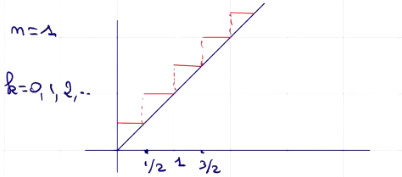
\includegraphics[width=0.6\linewidth]{screenshot011}
	\caption{These are screenshots taken from the video feed. I couldn't bother. Sorry.}
	\label{fig:screenshot011}
\end{figure}
But after $n=2$ we get the same function with smaller "steps":
\begin{figure}[H]
	\centering
	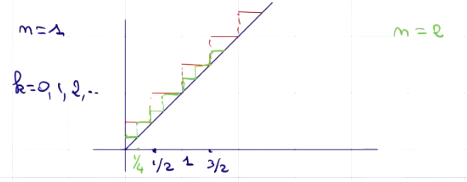
\includegraphics[width=0.6\linewidth]{screenshot012}
	\caption[The problem of improvisation]{The aesthetic problem of musical execution is reduced by Enrico Fubini to a problem of musical improvisation: I honestly think that this perspective is limiting both in its conceptions of ``execution'' and ``improvisation'' even if I agree with the intent of blurring the line between the two concepts unjustly separated in our Western modern musical. That is, a modern perspective: the reader will surely remember that Bach was famous first and foremost for his improvisational abilities and that the musical form of the fugue was often used to display pyrotechnical capabilities in that regard.}
	\label{fig:screenshot012}
\end{figure}
Observe that $d_1\geq d_2\geq d_3\geq\ldots$. What are the other properties of this function?
\begin{enumerate}
	\item it is a step function;
	\item it is right-continuous;
	\item $d_n(t)>t$ (the diagonal line);
	\item $\lim_{n\to\infty}d_n(t)=t$.
\end{enumerate}
Now we apply this simple function to our stopping times so that we get the following proposition.
\begin{proposition}
	Let $\F$ be a filtration on $\Rext_+$ and let $T$ be a stopping time. Let 
	\[T_n=d_n\circ T.\]
	Then ${\{T_n\}}_{n}$ is a sequence of \emph{discrete stopping times} of $\F$ decreasing to $T$.
\end{proposition}
\begin{remark}
Of course $T_n$ is a foretold time by $T$, because if I know $T$ I also know the value of $T_n$.
\end{remark}
\begin{fancyproof}
	Fix $n$:
	\begin{itemize}
		\item $T_n$ is a measurable function of $T\implies T_n\in\F_n$;
		\item $d_n(t)\geq t\quad\every t<\infty$ and $d_n(\infty)=\infty\implies d_n(T)=T_n\geq T$;
		\item $T_n$ is a foretold time by $T$;
		\item $T_n$ is a stopping time;
		\item $T_n$ is discrete.
	\end{itemize}
	But $d_n(t)\searrow t$ as $n\to\infty\implies d_n(T)=T_n\searrow T$. We have thus switched from a continuous stopping time to a sequence of discrete stopping times.
\end{fancyproof}
An important thing to note is that during our process of discretization we never break the property of the stopping times... and this is possible because we are using foretold times!
\subsection{Conditioning at stopping times}
Imagine that we have our information about $X$ that stops at the stopping time $T$: this means knowing $\F_T$. Consider the classic conditioning situation
\[\ev(X\F_T).\]
We already said how this is our best estimate of $X$ using our information available (that is $\F_T$).
\begin{notation}
	We will write
	\[\ev_T\equiv\ev_{\F_T}\equiv\ev(\cdot|\F_T).\]
\end{notation}
\begin{remark}
	Can I use $T$ fixed as a deterministic time $t$ and thus get $\ev(X|\F_t)$? Is this a special case or a different think altogether? Well yes, because $t$ \textit{is} a stopping time being $\F_t$-measurable! $\ev(X|\F_t)$ is a special case of $\ev(X|\F_T)$.
\end{remark}
This becomes clear when we see the properties of stopped expectation. For $\every X,Y,Z$ being positive \rv s and for $\every S,T$ stopping times of $\F$ the following properties hold:
\begin{itemize}
	\item \emph{defining property}:
	\[\ev_T X=Y\iff V\in\F_T\text{ and }\ev VX=\ev VY;\]
	\item \emph{unconditioning}:
	\[\ev\ev_T X=\ev X;\]
	\item \emph{repeated conditioning}:
	\[\ev_S\ev_T X=\ev_{\min\{S,T\}}X=\ev_{S\wedge T}X;\]
	\item \emph{conditional determinism}:
	\[\ev_T(X+YZ)=X+Y\ev_T(Z)\]
	if $X,Y\in\F_T$.
\end{itemize}
We need to prove the third property.
\begin{fancyproof}
	Notice that if $S\leq T\implies\F_S\subset\F_T$. This means that 
	\[\ev_S\ev_T=\ev_S\left(=\ev_{S\wedge T}\right)\]
	(the ``poorer'' \sa{} wins!). Moreover notice that if $S$ and $T$ are arbitrary we can apply the same result to $S\wedge T$ since $S\wedge T\leq T$ and 
	\begin{equation}
		\ev_{S\wedge T}\ev_{T}=\ev_{S\wedge T}\tag{$\bullet$}\label{stopexpect}
	\end{equation}
	Remember that $Y=\ev_T X$. Let's now try to write the statement of our proof in a different way:
	\[\ev_S Y=\ev_{S\wedge T}X.\]
	But using our property (\ref{stopexpect}) we get
	\begin{align*}
		\ev_S Y&=\ev_{S\wedge T}\ev_T X\\
		&=\ev_{S\wedge T} Y.
	\end{align*}
	Let's prove this, by steps.
	\begin{enumerate}
		\item note that $\F_{S\wedge T}\subset\F_S$. This means that $\ev_{S\wedge T}Y$ is in $\F_S$ and therefore $\ev_{S\wedge T}Y $ has the measure property and it is a candidate to be $\ev_S Y$. So we should check whether this candidate satisfies the defining property of stopped expectation.
			\item Check the defining property
			\[\ev VY=\ev V\ev_{S\wedge T}Y\]
			for each positive $V$ in $\F_S$. We start by fixing such $V$, positive and in $\F_S$. We proved that 
			\[V\indi_{\{S\leq T\}}\in\F_{S\wedge T}\]
			and the defining property for $\ev_{S\wedge T}$ gives
			\begin{equation}
				\ev V\indi_{\{S\leq T\}}Y=\ev V\indi_{\{S\leq T\}}\ev_{S\wedge T}Y\tag{$\bullet\bullet$}\label{hateproof}
			\end{equation}
			Now we observe that $Y\in\F_T$ by definition. Also notice that $Y\indi_{\{T<S\}}\in\F_{S\wedge T}$. Apply now this fact to the defining property and obtain
			\begin{equation*}
				\ev VY\indi_{\{T<S\}}=\ev V\ev_{S\wedge T}Y\underbracket{\indi_{\{T<s\}}}_{\mathclap{\F_{S\wedge T}\text{-meas.}}}
			\end{equation*}
			and by conditional determinism we get
			\begin{align*}
				\ev VY\indi_{\{T<S\}}&=\ev V\indi_{\{T<S\}}\\
				&=\ev V\indi_{\{T<S\}}\ev_{S\wedge T}Y.
			\end{align*}
			By putting together this result with (\ref{hateproof}) we get
			\begin{equation*}
				\ev V Y=\ev V\ev_{S\wedge T}Y.
			\end{equation*}
	\end{enumerate}
\end{fancyproof}
\section{Martingales}
When we study stochastic processes, the typical way of introducing classes of stochastic processes for which we have methods to study is determining the finite dimensional distributions. If we have them, thanks to the Kolmogorov Consistency theorem, we can give a complete description of the process but this is boring and for fucking losers. So we introduce classes of stochastic processes for which we can write the distribution.\par
Imagine, from a different view point, another approach: instead of starting from the distribution of a stochastic process we start from a property; then as a consequence of that property we infer the behavior towards infinity. This is the philosophy behind the class of \emph{martingales}.
\begin{example}
	Consider the process $\{X_{n}\}$ that describes the fortune of a player. This player wins with probability $p$ and loses with probability $1-p=q$. Consider the fortune at time $n$ ${\{S_n\}}_{n\geq 0}$, which is 
	\[S_n=\sum_{i=0}^{n}X_i.\]
\end{example}
	Is the game fair? Imagine also that the $X_i$'s are the value that I get by losing or selling options or stock. We know that the game is fair if $p=q=\frac{1}{2}$. But this could also be written as a property in the following way:
	\[\ev\left[S_{n+1}|\underbracket[0.64pt]{S_n}_{\F_n}\right]=S_n.\]
	So I don't have any ``advantages'' or ``bias''.
	\begin{fancyproof}
		\begin{align*}
			\ev\left[S_{n+1}|S_n\right]&=\ev\left[S_n+X_{n+1}|S_n\right]\\
			&=S_n+\ev\left[X_{n+1}|S_n\right]\\
			&=S_n+\underbracket[0,6pt]{\ev\left[X_{n+1}\right]}_{\mathclap{=0\text{ if }p=q=\frac{1}{2}}}\\
			&=S_n
		\end{align*}
	\end{fancyproof}
We will not define martingales through the event/filtration that allows the process $Y$ to remain constant:
\[\ev[Y_{n+1}|\F_n]=Y_n.\]
Then we should ask some questions about this \sa. We know that $\{\F_n\}$ can be increasing, constant or decreasing but $Y$ must remain constant in mean. Look at it through the tower property.
\[\ev Y_n=\ev\left[\ev\left[Y_{n+1}|\F_n\right]\right]=\ev Y_{n+1}.\]
\begin{definition}
	A real-valued process
	\[X={(X_t)}_{t\in\T}\]
	is called a \emph{$\F$-martingale} if:
	\begin{enumerate}
		\item it is adapted to $\F$;
		\item it is integrable for each $t\in\T$;
		\item $\ev(X_t-X_s|\F_s)=0\quad\every s<t$.
	\end{enumerate}
	If $\ev(X_t-X_s|\F_s)\geq0\quad\every s<t$ then the process is called \emph{$\F$-submartingale} and if $\ev(X_t-X_s|\F_s)\leq0\quad\every s<t$ it is called \emph{$\F$-supermaringlae}.
\end{definition}
These three properties are what we need to check to establish whether a process has martingale properties. The first two are really just regularity conditions, while the third is the ``real'' defining property of a martingale. There is is another definition for the third property:
\begin{definition}
	\begin{enumerate}
		\item[3'.] $\ev(X_t|\F_s)=X_s$.
	\end{enumerate}
\end{definition}
In the first definition we were looking at the increment, now we are looking at the mean of a further point $t$ in time for the process $X$ and discovering that, conditioning it to information available in time $s$, it doesn't change from the process in time $s$.\\
If $\ev X^{+}_{t}<\infty$ then the sequence $\{X_t\}$ (that can be a sub-martingale) converges to a limit. 
\begin{remark}
	A martingale is also a sub-martingale and a super-martingale.
\end{remark}
We will use sub-martingales in our demonstrations but it really does not change anything because if $\{X_t\}$ is a $\F$-sub-martingale then $\{-X_t\}$ is a $\F$-super-martingale.
\begin{remark}
	The number of terms in $\{X_t\}$ can be bounded or unbounded: even a process with 4 terms can be a martingale.
\end{remark}
There are consequence to the way we defined martingales. Consider the times $s<t<u$ and the $\F$-martingale $\{X_t\}$. Then
\[\ev_s(X_u-X_{t})\]
means knowing the evolution of the process at time $s$ and looking for the increment of the process between $t$ and $u$. 
\begin{figure}[H]
	\centering
	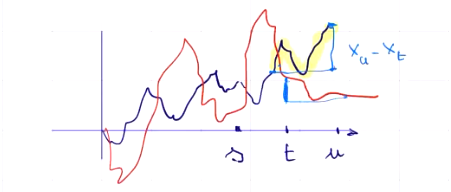
\includegraphics[width=0.7\linewidth]{screenshot013}
	\caption{It should not}
	\label{fig:screenshot013}
\end{figure}
We can write
\begin{align*}
	\ev_s(X_u-X_{t})&=\ev_s\Big(\underbracket[0.56pt]{\ev_t(X_u-X_t)}_{\mathclap{=0\text{ bc it is a martingale}}}\Big)\\
	&=\ev_s 0=0.
\end{align*}
This means that given the information up to time $s$ the estimation of any future increment will be null! In the special case $\T=\N$ then this property becomes
\[\ev_n(X_{n+1}-X_n)=0.\]
\begin{proposition}
	If $\{X_i\}$ is an $\F_n$-martingale, it holds
	\[\begin{array}{l l}
		\ev X_i=\ev X_{i+1}&\text{if it is a martingale}\\
		\ev X_{i+1}>\ev X_i&\text{if it is a sub-martingale.}
	\end{array}\]
\end{proposition}
\begin{fancyproof}
	Consider the expectation
	\[\ev(X_{i+1}|\F_i)\geq X_i\]
	being a sub-martingale. Take the expectation
	\[\underbrace{\ev\left[\ev(X_{i+1}|\F_i)\right]}_{\ev X_{i+1}}\geq\ev X_i.\]
	We can now define the process
	$\{Y_{i}\}_{i\in\N}$ as 
	\[Y_{i+1}=X_{i+1}-X_{i}.\]
	We know that $\{X_i\}$ is a $\F$-martingale. Note that
	\[\sum_{j=1}^{i} Y_j=X_1-X_0+X_2-X_1+\ldots+X_i-X_{i-1}\]
	so that we can write
	\[X_i=c+\sum_{j=1}^{i}Y_j.\]
	We know that 
	\[\ev\left[X_{i+1}|\F\right]=X_i\]
	But we also know that 
	\begin{equation*}
	\ev[Y_{i+1}|\F]=0.
	\end{equation*}
\end{fancyproof}
The quantity $\{\ev{Y_{i+1}|\F_i}\}$ is called \emph{martingale difference}.
\begin{example}
	Imagine we have a sequence $\{Y_i\}$ of independent \rv s with $\ev Y_i=0$.
	Consider $\F_1$, the \sa{} generated by $\{Y_j,0\leq j\leq i\}$. Call $S_i=c+\sum^{i}Y_{j}$. 
	$\{S_i\}$ is an $\F$-martingale.
\end{example}
\subsection{Properties of martingales}
\begin{enumerate}
	\item Consider $X$ and $Y$ being $\F$-sub-martingales and $a,b\in\R^{+}$. Then 
	\[aX+bY\]
	is a $\F$-sub-martingale.
	\item Consider $X,Y$ being two $\F$-sub-martingales. Then
	\[\max\{X,Y\}\]
	is a $\F$-sub-martingale.
	\begin{fancyproof}
		Consider $\ev[\max\{X_{n},Y_{n}|\F_{n-1}\}]$. Remember that we have to prove: \begin{itemize}
			\item measurability property;
			\item integrability property;
			\item martingale property.
		\end{itemize}
		Often times measurability and integrability are implied in the form of the function.  Since we are using the maximum between $X$ and $Y$ we know that
		\[\begin{array}{l}
			\ev[\max\{X_{n},Y_{n}|\F_{n-1}\}]\geq\ev[X_{n}|\F_{n-1}\}]\\
			\ev[\max\{X_{n},Y_{n}|\F_{n-1}\}]\geq\ev[Y_{n}|\F_{n-1}\}].
		\end{array}\]
		But since $X$ and $Y$ are martingales we know that $\ev[X_{n}|\F_{n-1}]\geq X_{n-1}$ and $\ev[Y_{n}|\F_{n-1}]\geq Y_{n-1}$; hence we get that
		\[\ev[\max\{X_{n},Y_{n}|\F_{n-1}\}]\geq\max\{X_{n-1},Y_{n-1}\}\]
		so the martingale property is satisfied.
	\end{fancyproof}
	\item Consider two $\F$-super-martingales $X_{n},Y_{n}$. Then
	\[\min\{X_{n},Y_{n}\}\]
	is a $\F$-super-martingale.
	\begin{fancyproof}
		Consider $\max\{-X_{n},-Y_{n}\}$. We know that $-X_n$ is a sub-martingale and so is $-Y_{n}$. So as proved above $\max\{-X_{n},Y_{n}\}$ is a sub-martingale. But $\max\{-X_{n},-Y_{n}\}=-\min\{X_{n},Y_{n}\}$ so
		\[-\min\{X_{n},Y_{n}\}\text{ is a sub-martingale}\iff\min\{X_{n},Y_{n}\}\text{ is a super-martingale}.\]
	\end{fancyproof}
	\item Consider a function $f$ that is \underline{convex} on $\R$. If $X$ is a $\F$-martingale and $f\circ X$ is integrable then $f\circ X$ is a $\F$-sub-martingale.
	\begin{fancyproof}
		We have $s<t$ and we want to study $\ev\left[f(X_{t})|\F_{s}\right]$. By Jensens's inequality we have
		\begin{align*}
			\ev\left[f(X_{t})|\F_{s}\right]&\geq f\Big[\underbrace{\ev(X_{t}|\F_s)}_{X_s}\Big]\\
			&=f(X_s).
		\end{align*}
	\end{fancyproof}
	\begin{remark}
		Some examples of positive functions of $X$ are $X^{+},X^{-},|X|$. If $X$ is martingale, these are sub-martingales.  $|X|^{p}$ is a sub-martingale if $X$ is a martingale and $\ev|X|^{p}<\infty$.
	\end{remark}
	\item if $f$ is convex and increasing and $X$ is a $\F$-sub-martingale with $f(X_{t})$ integrable $\every t$ then $f(X_{t})$ is again a $\F$-sub-martingale.
\end{enumerate}
\subsection{Create your own martingale}
\begin{enumerate}
	\item Consider an increasing family of \sa s $\{\F_j\}$ and a \rv{} $X$ on $(\Omega,\F,\pr)$ which is integrable and adapted to $\F$.
	Define 
	\[X_i=\ev[X|\F_i].\]
	Then the process ${\{X_i\}}_{i\in\N}$ is called \emph{Doob martingale} and plays an important role in may processes. As $i$ increases, so does the information about our random variable while retaining the underlying process $X$.\\
	We have now to prove that $\{X_i\}$ is a $\F$-martingale. 
	\begin{fancyproof}
		We need to check that \begin{align*}
			\ev[X_{i+1}|\F_{i}]&=\ev\left[\ev\left[X|\F_{i+1}\right]|\F_{i}\right]\\
			&=\ev\left[X|\F_{i}\right]
		\end{align*}
		and this is because of the properties of conditional expectation since $\F_{i+1}\supset\F_{i}$. But $\ev\left[X|\F_{i}\right]=X_i$ by definition.
	\end{fancyproof}
	The same result holds when $\T$ is continuous.
	\item Consider sums of independent \rv $\{X_i\}$ with $\ev[X_i]=0$. We have 
	\[S_0=0\qquad S_n=S_0+X_1+X_2+\ldots+X_{n}\qquad n\geq1.\]
	We define $\F={(\F_{n})}_{n\in\N}$ as the filtration generated by $S={(S_{n})}_{n\in\N}$. Consider the following facts:
	\begin{enumerate}
		\item $\F_{n}$ is adapted to $S$;
		\item Each $S_{n}$ is integrable and $\ev S_{n}=0$;
		\item $\ev_{n}(S_{n+1}-S_n)=\ev_n(X_{n+1})=\ev X_{n+1}=0$ (because of independence).
	\end{enumerate}
	So $S_{n}$ is a martingale.
	What happens, tough, if $\ev X_i=1$ for each $i$? We would get a sub-martingale (because we would have an increasing process).
	\item Consider the product of \rv s. Consider $R_1,R_2,\ldots$ being independent \rv s with
	\[\ev R_i=1\qquad\var R_i<\infty\]
	that don't necessarily need to be identically distributed. Let $M_{0}=1$ and $M_n=M_{0}\cdot R_{1}\cdot R_{2}\cdot\ldots\cdot R_{n}$ and let $\F$ be the filtration generated by $M={\{M_n\}}_{n\in\N}$. Observe that
	\begin{enumerate}
		\item $M$ is adapted to $\F$ by definition;
		\item $\every M_{n}$ is integrable: consider $\norm{M_{n}}\leq\norm{M_{n-1}}\norm{R_{n}}$ since $M_{n}=M_{n-1}R_{n}$. But since $R_{n}$ has finite variance then $\norm{M_{n-1}}\norm{R_{n}}<\infty$. So since it is bounded it is integrable;
		\item consider the expectation
		\begin{align*}
			\ev[M_{n+1}|\F_{n}]&=\ev[M_{n}R_{n+1}|\F_{n}]\\
			&=M_{n}\ev[R_{n+1}|\F_{n}] \qquad\text{(beacuse $M_n$ is $\F_n$-meas.)}\\
			&=M_{n}\ev[R_{n+1}]\\
			&=M_{n}.
		\end{align*}
	\end{enumerate}
	\begin{example}
		This is considered a good model for finance: $M_{n}$ is the price of a share at time $n$ and $R_{n+1}$ is the return at time $(n+1)$ per euro invested at time $n$. $\F_n$ is the information that is available to the whole market.
	\end{example}
	\item  Consider functions of sums. Consider $\{X_{n}\}$, a sequence of i.i.d. \rv s with
	\[\ev X_i=0\qquad\var X_i=\sigma^{2}<\infty\quad\every i.\]
	Consider
	\[S_{n}=\sum^{n}X_i\]
	and define
	\[M_{n}=S_{n}^{2}-n\sigma^{2}.\]
	$M_n$ is a $\F$-martingale. This is useful to study for example the occurrence of the time in which something happens for the first time. 
	Consider:
	\begin{enumerate}
		\item $M_{n}$ is integrable ($\var X_i=\sigma^{2}$);
		\item $M_{n}$ is adapted by definition;
		\item consider the expectation 
		\begin{align*}
			\ev[M_{n+1}|\F_{n}]&=\ev\Big[\underbracket[0.6pt]{(S_{n}+X_{n+1})^{2}}_{S^{2}_{n+1}}-(n+1)\sigma^{2}|\F_{n}\Big]\\
			&=\ev\Big[S_{n}^{2}+N_{n+1}^{2}+2S_{n}X_{n+1}-(n+1)\sigma^{2}|\F_{n}\Big]\\
			&=S_{n}^{2}+2S_{n}\underbracket[0.6pt]{\ev(X_{n+1}|\F_{n})}_{=0}+\underbracket[0.6pt]{\ev[X_{n+1}^{2}|\F_{n}]}_{\mathclap{\ev[X^{2}_{n+1}]=\sigma^{2}}}-(n+1)\sigma^{2}\\
			&=S_{n}^{2}+\cancel{\sigma^{2}}-n\sigma^{2}-\cancel{\sigma^{2}}=M_{n}.
		\end{align*}
	\end{enumerate}
	\begin{example}
		Consider ${(X_{n})}_{n\geq 1}$ being i.i.d. \rv s with common probability density function $g(x)$. Let $f(x)$ be another probability density function with the property
		\[f(x)=0\qquad\text{for }\frac{x}{g(x)}=0.\]
		Define
		\begin{equation*}
			\begin{array}{l l}
				L_n&=\underbracket{\prod_{i=1}^{n}\frac{f(X_i)}{g(X_{i})}}_{\mathclap{\text{likelihood ratio}}}\\
				L_0&=1.
			\end{array}
		\end{equation*}
		Likelihood ration is a $\F$-martingale where $\F$ is the filtration generated by $\{X_{n}\}$. Contemplate:
		\begin{enumerate}
			\item it is integrable by definition;
			\item it is adapted by definition;
			\item consider the expectation:
			\begin{align*}
				\ev\Big[L_{n+1}|\F_{n}\Big]&=\ev\left[L_{n}\frac{f(X_{n+1})}{g(X_{n+1})|\F_{n}}\right]\\
				&=L_{n}\ev\left[\frac{f(X_{n+1})}{g(X_{n+1})}|\F_{n}\right]\qquad\text{(beacuse $L_n$ is $\F_n$-meas.)}\\
				&=L_{n}\ev\left[\frac{f(X_{n+1})}{g(X_{n+1})}\right]\\
				&=L_{n}\underbrace{\int_{\R}\frac{f(X)}{\cancel{g(X)}}\cancel{g(x)}}_{=1}\dx=L_{n}.
			\end{align*}
		\end{enumerate}
	\end{example}
\end{enumerate}
This really is exhausting. Like it literally drains the life from me
\subsection{Doob's decomposition}
We may want to understand whether there is any relationship between a stochastic process and a martingale. In this part our set $\T$ will be $\N$.\\
Up to now we said that a process is adapted to $\F$ if $X_{n}$ is $\F_n$-measurable. 
\begin{definition}
	The process $F={(F_{n})}_{n\geq1}$ is \emph{$\F$-predictable} if $F_{0}\in\F_{0}$ and $\F_{n+1}\in\F_{n}$, for $\every n\in\N$.
\end{definition}
This means that the available information up to $n$ is ``enough'' to have a bet in the period $n+1$. Some predictable processes are:
\begin{itemize}
	\item any deterministic processes;
	\item consider two stopping times $S,T$ of $\F$ and let $S\leq T$. Consider the \rv{} $V$ in $\F_{n}$. Then
	\[\begin{array}{c c c c}
	\color{DodgerBlue3}(1)&\color{DodgerBlue3}(2)&\color{DodgerBlue3}(3)&\color{DodgerBlue3}(4)\\
		V\indi_{(S,T]}&V\indi_{(S,\infty]}&\indi_{(S,T]}&\indi_{(0,T]}
	\end{array}\]
	are predictable processes.
	\begin{fancyproof}
		\begin{enumerate}
			\item[\color{DodgerBlue3}(2)] Consider $F=V\indi_{(S,\infty]}$, so that $F_{n}=\indi_{(S,\infty]}(n)$. Consider \begin{align*}
				F_{n+1}&=V\indi_{(S,\infty]}(n+1)\\
				&=V\indi_{\{S<n+1\}}\\
				&=V\indi_{\{S\leq n\}}\in\F_{n}
			\end{align*}
			so the process is $\F$-measurable and predictable.
			\item[\color{DodgerBlue4}(1)] Since we know by hypothesis that $S\leq T$ then $V\in\F_{S}\subset\F_{T}$. This means that $V\in\F_{T}$. Hence, of a consequence,
			\begin{equation*}
				V\indi_{(T,\infty]}-V\indi_{(S,\infty]}=V\indi_{(S,T]}
			\end{equation*}
			is predictable.
			\item[\color{DodgerBlue3}(3)] Take $V=1$.
			\item[\color{DodgerBlue3}(4)] Take $T=\infty$, $V=1$. $\indi_{(S,\infty]}$ is predictable. But then 
			\[\indi_{[0,S]}=\indi-\indi_{(S,\infty]}\]
			so it is predictable.
		\end{enumerate}
	\end{fancyproof}
\end{itemize}
\begin{theorem}
	\emph{Doob's decomposition}.\\
	$X$ is a stochastic process which is adapted to $\F$ and integrable. Then
	\begin{enumerate}
		\item it can be decomposed as 
		\[X_{n}=X_{0}+M_{n}+A_{n},\qquad n\in\N\]
		where:
		\begin{itemize}
			\item $M_{n}$ is a $\F$-martingale with $M_0=0$;
			\item $A_{n}$ is a predictable process with $A_0=0$.
		\end{itemize}
		\item The decomposition is unique up to equivalence.
		\item If $X_{n}$ is a sub-martingale then ${\{A_{n}\}}_{n\geq0}$ increasing, while if $X_{n}$ is a super-martingale then ${\{A_{n}\}}_{n\geq0}$ is decreasing.
	\end{enumerate}
\end{theorem}
\begin{fancyproof}
	Put $A_0=M_0=0$. Define $M$ and $A$ through their increments:
	\[ \begin{array}{l l}
		A_{n+1}-A_{n}&=\underbracket[0.3pt]{\ev\Big[X_{n+1}-X_{n}|\F_{n}\Big]}_{\F_{n}-\text{meas.}}\\
		M_{n+1}-M_{n}&=(X_{n+1}-X_{n})-(A_{n+1}-A_{n}).
	\end{array} \]
	If we look at these quantities we see that $A$ is predictable and $M$ is martingale. Imagine now there is another decomposition: let
	\[X=X_0+M'+A'\]
	be another decomposition. We must have
	\[\cancel{X_0}+M'+A'=\cancel{X_0}+M+A\iff A-A'=M-M'=B.\]
	Now $B$ is a process and it is predictable and martingale (because it is the difference between two martingales). Since $B$ is predictable \textit{and} a martingale we have
\begin{align*}
			B_{n+1}-B_{n}&\underset{\mathclap{\text{\tiny predictable}}}{=}\ev[B_{n+1}-B_{n}|\F_{n}]\\
		&\underset{\mathclap{\text{\tiny martingale}}}{=}0\\
		&\implies B_{n+1}=B_{n}=B_0\;\as,A=A'\;\as,M=M'\as\\
\end{align*}
If $X$ is a sub-martingale then we have
\[\ev[X_{n+1}-X_{n|\F_{n}}]\geq0\]
and this means that we have $A_{n+1}\geq A_{n}$ is increasing.
\end{fancyproof}
Consider the increments on $X$:
\[X_{n+1}-X_{n}=\underbrace{A_{n+1}-A_{n}}_{\mathclap{\text{prediction term}}}+\underbrace{M_{n+1}-M_{n}}_{\mathclap{\text{innovation}}}.\]
Engineers, much better people than us, often use this terms.
\subsection{Important stochastic processes and related martingales}
A quick note before starting:
\subsubsection*{Markov chains}
Consider a stochastic process ${\{X_{n}\}}_{n\geq 1}$. All trials are on the same probability space $(E_n,\E_{n})=(E,\E)$. Define a \emph{Markov kernel} on $(E,\E)$
\[(E,\E)\mapsto(E,\E)\]
such that
\[K_{n}(x_{0},x_{1},\ldots,x_{n};A)=\pr(x_{n},A)\qquad\every n\in\N,\;\every(x_{0},x_{1},\ldots,x_{n})\in E,A\in\E.\]
So the probability that governs the evolution is dependent \textit{only} on the last state and nothing else. If $x_{n+1}=j,x_{n}=i$ then $\pr(i,j)=p_{ij}$. The process $X={\{X_{n}\}}_{n\geq0}$ is said to be a \emph{Markov chain} over $(\Omega,\HS,\pr)$ with state space $(E,\E)$, initial distribution $\mu$ and transition kernel $P$.\\
\[P={(p_{ij})}_{i,j}\]
Now consider a Markov chain with transition probability matrix $P$ such that
\[P\cdot\underbrace{f}_{{\text{eigenvector}}}=\underbrace{\lambda}_{{\text{eigenvalue}}}\cdot f.\]
This means that we have the following system of equations:
\[\begin{cases}
	\sum_{j} p_{ij}f(j)=\lambda f(i)&i=1\\
	\vdots&i=2\\
	\vdots&\vdots.
\end{cases}\]
We can clearly write these expressions in form of expectation:
\[\ev[f(X_{n+1})|X_{n}=i]=\lambda f(i).\]
We can also write it without fixing $i$:
\begin{equation}
	\ev[f(X_{n+1})|X_{n}]=\lambda f(X_{n}).\tag{$\bullet$}\label{markovbitch}
\end{equation}
Look at the last equation: it is not too different from the martingale property. Consider the ratio $\frac{f(X_{n})}{\lambda^{n}}$ and the filtration generated by $X$ $\sigma(X_{0},X_{1},\ldots,X_{n})$. Thanks to the relation given by the equation (\ref{markovbitch}) it is a martingale with respect to $\sigma(X_{0},X_{1},\ldots,X_{n})$.
\begin{fancyproof}
	Consider the expectation 
\begin{align*}
		\ev\left[\frac{f(X_{n+1})}{\lambda^{n+1}}\Big|X_0,\ldots,X_n\right]&=\frac{1}{\lambda^{n}}\frac{1}{\lambda}\underbrace{\ev\left[f(X_{n+1}|X_{n})\right]}_{\lambda f(X_{n})}\\
		&=\frac{1}{\lambda^{n}}\frac{1}{\cancel{\lambda}}\cancel{\lambda}f(X_{n})\\
		&=\frac{1}{\lambda^{n}}f(X_{n})\\
		&=Y_{n}
\end{align*}
where the first equality is thanks to Markov property. This is a general property for Markov chains.
\end{fancyproof}
\begin{example}
	\emph{Branching processes}. We study the life of a generation of individual. 
	\begin{figure}[H]
		\centering
		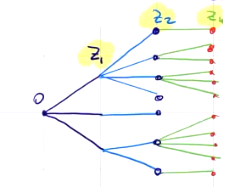
\includegraphics[width=0.5\linewidth]{screenshot015}
		\caption{I don't even know anymore.}
		\label{fig:screenshot015}
	\end{figure}
	The offsprings have a distribution $\{p_{k}\}$. The mean number of offsprings per individual is $m=\sum kp_{k}$. Consider the i.i.id \rv s $\{Z^{(n)}(i),n\geq 0\}$ describing the number of children of the $i$-th individual of generation $n$. Define 
\begin{equation*}
	Z_{n+1}=\begin{cases}
		Z^{(n)}(1)+Z^{n}(2)+\ldots+Z^{(n)}(Z_{n})&\text{if }Z_{n}\neq 0\\
		0&\text{if }Z_{n}=0
	\end{cases}
\end{equation*}
We immediately realize that this is a Markov process because every generation's number of children can be entirely derived from the previous generation's law or reproduction. I don't need to know whose child the individual is. So $Z_{n}$ (number of individual of the $n$-th generation) gives rise to a Markov chain. 
\begin{equation*}
	\sum_{j=0}^{\infty}p_{ij}j=m\cdot i
	\end{equation*}
	Is the equation that tells us the complete number of individuals. Now consider $Pf=mf$ with $f(j)=j$. So we have $Pj=mi$ where $m$ plays the role of $\lambda$. The process $\{\frac{Z_{n}}{m^{n}},\sigma(Z^{(0)},\ldots,Z^{(n)})\}$ is a martingale. 
\end{example}
\subsubsection*{Poisson martingale}
Consider $\R_{+}$ as our index set. $\F$ is our filtration and we consider the counting process $N={(N_{t})}_{t\geq 0}$ (it counts the number of events up to time $t$). It has unit jumps and any path starts from 0 ($N_0(\omega)=0$), is increasing and right continuous.
\begin{definition}
	The counting process $N$ is said to be a \emph{Poisson process} with rate $\lambda$ with respect to $\F$ if it is adapted to $\F$ and
	\[\ev[f(N_{t+s}-N_s)|\F_s]=\sum_{k=0}^{\infty}e^{-\lambda t}\frac{(\lambda t)^{k}}{k!}f(k)\qquad\every s,t\in\R_+,\every\text{positive }f\mapsto\N.\]
\end{definition}
\begin{theorem}
	Let $N$ be a counting process. It is a Poisson process with rate $\lambda$ with respect to $\F$ \ifonly{}:
	\begin{equation*}
		M_{t}=N_{t}-\lambda t
	\end{equation*}
	is a $\F$-martingale.
\end{theorem}
We only prove that $M_t$ is a martingale if $N_{t}$ is Poisson.
\begin{fancyproof}
	We know that 
	\begin{align*}
		\ev[M_{t}|\F_{s}]&=\ev[M_{t}-M_{s}+M_{s}|\F_{s}]\\
		&=\ev[M_{t}-M_{s}|\F_{s}]+M_{s}\\
		&=\ev[M_{t}-M_{s}]+M_{s}\\
		&=\ev[N_{t}-N_{s}+\lambda t+\lambda s]+M_{s}\\
		&=\underbrace{\ev[N_{t}-N_{s}]}_{\cancel{\lambda (t-s)}}-\cancel{\lambda (t-s)}+M_{s}\\
		&=M_{s}
	\end{align*}
\end{fancyproof}
We may use the Doob's decomposition theorem to get $N_{t}=M_{t}+\lambda t$ where $\lambda t$ is our predictable process. So the same result can be achieved from two different viewpoints.
\subsection{Integration in discrete time}
Let us consider two real-valued processes $M={(M_{n})}_{n}$ and $F={(F_{n})}_{n}$ and let us define
\[X_{n}=F_0M_{0}+(M_1-M_0)F_1+\ldots+(M_{n}-M_{n-1})F_n.\]
We say that $\{X_{n}\}$ is the integral of $F$ with respect to $M$ and we write
\[X_{n}=\int F \dif M\]
where $\dif M$ is a random signed measure. Remember the Lebesgue-Stieltjes integral? Me neither, but as long as $M$ has bounded variation this is a Lebesgue-Stieltjes integral.
	\begin{flushright}
		\begin{tikzpicture}
			\calloutquote[width=4cm,position={(1,-1)},fill=Turquoise4!30,rounded corners]{Yeah no wait hold your fucking horses.}
		\end{tikzpicture}\hspace*{2.5cm}
	\end{flushright}
	\hspace{2cm}
	\begin{tikzpicture}
		\calloutquote[width=3cm,position={(-1,-1)},fill=DodgerBlue4,rounded corners]{\color{white}What's up now?}
	\end{tikzpicture}
		\begin{flushright}
		\begin{tikzpicture}
			\calloutquote[width=5cm,position={(1,-1)},fill=Turquoise4!30,rounded corners]{First of all how is that shit an integral?? And what the fuck is a Lebesgue-Stieltjes integral?}
		\end{tikzpicture}\hspace*{2.5cm}
	\end{flushright}
	\hspace{2cm}
	\begin{tikzpicture}
		\calloutquote[width=5cm,position={(-1,-1)},fill=DodgerBlue4,rounded corners]{\color{white}I should have NEVER let you enroll in this master.}
	\end{tikzpicture}
	\begin{flushright}
		\begin{tikzpicture}
		\calloutquote[width=5cm,position={(1,-1)},fill=Turquoise4!30,rounded corners]{Professor Lods, I will exact my revenge on Università di Torino very soon.}
	\end{tikzpicture}\hspace*{2.5cm}
	\end{flushright}
	Okay okay. So a little explanation is due since I actually never saw a Stieltjes integral. Too busy doing things, y'know. Things like, for example, sex. Heh. Yeah. Sex. 
\begin{revise}
	Oookay so very shortly: a Riemann-Stieltjes integral is a generalization of our dear old Riemann integral. It is notated as
	\begin{equation*}
		\int_{a}^{b}f(x)dg(x).
	\end{equation*}
	Actually this is not too different from the concept of the Lebesgue integral. Basically is about partitioning the interval $(a,b)$ and then summing for every partition (that is, for each $i$) each value of $f(x_i)$ multiplied for $[g(x_i)-g(x_{i-1})]$. Just take the limit for the partition to be infinitely small and voilà, le integràl c'est servie (I don't know French). El integral està servido (I know a little bit of Spanish). Omnibus integral paratum est ut facile intellegatur (I actually know Latin really well. Useless skills are my strength).\par
	Anyway what's important is: \textit{we take the function $f(x)$ and use it to calculate how much the variation of $g(x)$ impacts on the total sum}. And if $g(x)=x$, well... We have our cute little Riemann integral!
\end{revise}
Yeah after this smug declaration of sterile knowledge we are maybe ready to better understand how the discrete time integral is, well, an integral. Our function $g(x)$ is $M$ so we consider the variation of $M$; since we are working in discrete time we will never reach a partition so fine it can be called continuous. So it's like... a \textit{diet} Riemann-Stieltjes integral.
\begin{theorem}
	Consider $F$ bounded and predictable. Then if $M$ is a martingale then $X$ is a martingale; If $M$ is a sub(super)-martingale then $X$ is a sub(super)-martingale.
\end{theorem}
This means that... \emph{we can't beat the system!}
	\begin{flushright}
	\begin{tikzpicture}
		\calloutquote[width=4cm,position={(1,-1)},fill=Turquoise4!30,rounded corners]{I can beat something else though.}
	\end{tikzpicture}\hspace*{2.5cm}
\end{flushright}
\begin{example}
	Consider $M_{n}$ as the price of a share at time $n$ and $F_{n}$ as the number of shares owned during $(n-1,n]$. Our profit will be 
	\[(M_{n}-M_{n=1})F_{n}\]
	and our total profit $X_{n}$ gained during $(0,n]$ will be:
	\[X_{n}=X_{0}+\underbrace{\sum_{k=1}^{n}(M_{k}-M_{k-1})F_{k}}_{\mathclap{\text{discrete time integral}}}\]
	$F_{n}$ is based on the knowledge in $n-1$ so it is predictable. The process $M_{n}$ should be a martingale (otherwise if it is a sub/super-martingale everyone/no one will buy). So the total profit will also be a martingale! We can only choose our buying politics $F_{k}$, but there is no way to select a politics that will change a martingale in a super-martingale or sub-martingale.
\end{example}
Clearly this works in mean! 
\begin{fancyproof}
\begin{enumerate}
	\item	We have $M$ being a martingale and $F_0,F_1,\ldots,F_n\in\F_{n}$ as well as $M_0,M_1,\ldots,M_{n}\in\F_n$. Therefore $X_{n}\in\F_{n}$ and $X$ is adapted to $\F$.
	\item We need to check whether the discrete time integral is a martingale. We know by hypothesis that $F$ is bounded, so $F<b$ for some $b$. This implies
	\begin{equation*}
		|X_{n}|<b(|M_{0}|+|M_1+M_0|+\ldots+|M_n-M_{n-1}|)
 	\end{equation*}
	Since $M$ is a martingale and it is integrable, we get that $X_n$ is bounded and integrable.
	\item Consider
	\begin{equation*}
		\ev[X_{n+1}-X_{n}|\F]=\ev[F_{n+1}(M_{n+1}-M_{n})|\F_n]
	\end{equation*}
	since all the terms cancel out and only the last ones survive. But $F_{n+1}\in\F_{n}$ so we can take it out of the expectation:
	\[F_{n}\underbrace{\ev[M_{n+1}-M_{n}|\F_{n}]}_{=0}=0.\]
\end{enumerate}
\end{fancyproof}
We know that using a policy that it is predictable it is impossible to beat the system. Finance bros try to overcome this possibility using stopping times. If my policy is not only based on a predictable process but I add the randomness of the time in which I decide to sell or buy can I break the curse of martingales and make shareholders want to suck my dick? Well, it depends.
\subsection{Stopped martingales and Doob's stopping theorem}
\begin{definition}
	Define $M={(M_{n})}_{n\in\N}$ as a process and let $T$ be a random time with values on $\overline{\N}$. The process
	\[X_{n}(\omega)=M_{n\wedge T}(\omega)=\begin{cases}
		M_{n}(\omega)&n<T(\omega)\\
		M_{T}(\omega)&n>T(\omega)
	\end{cases}\]
	(where $n\wedge T$ is a truncated random time) is called \emph{$M$ stopped at $T$}.
\end{definition}
As a consequence $X$ is exactly the discrete time integral if $F=\indi_{[0,T]}$:
\begin{equation*}
	X_{n}=\underbracket[0.6pt]{M_0F_0}_{0}+(M_{1}+M_{0})\indi_{[0,T]}(1)+\ldots+(M_{n}-M_{n-1})\indi_{[0,T]}(n).
\end{equation*}
The indicators only select the current time interval. If this is the case we can observe that $F_{[0,T]}$ is bounded, positive and predictable. Hence if $M$ is a martingale the theorem applies with this special choice of $M$ and we can write the result as a different theorem:
\begin{theorem}
	Let $T$ be a stopping time and let $X$ be the process $M$ stopped at $T$. If $M$ is a martingale then so is $X$ (the same holds for sub-martingales and super-martingales).
\end{theorem}
So we cannot determine a policy based on stopping times that can change the nature of our martingale. In the remote case in which you are interested in this you can read Williams - Introduction to martingales. \\
A further theorem about this is \emph{Doob's stopping theorem}. For a martingale we know
\[\ev[X_{t}-X_{s}|\F_{s}]=0.\]
The question is: is this true also if $s$ and $t$ are substituted by stopping times $S,T,S\leq T$?
\begin{theorem}
	Let $M$ be adapted to $\F$. Then the following are equivalent:
	\begin{enumerate}[\circnum]
		\item $M$ is a submartingale;
		\item for every bounded stopping time $S\leq T$ the \rv s $M_{S}$ and $M_{T}$ are integrable and 
		\[\ev[M_{T}-M_{S}|\F_{S}]\geq0;\]
		\item for each pair of bounded stopping times the \rv s $M_{S}$ and $M_{T}$ are integrable and 
		\[\ev[M_{T}-M_{S}]\geq 0.\] 
	\end{enumerate}
\end{theorem}
\begin{remark}
	If $M$ is a martingale the theorem can be read in a different way:
	\begin{equation*}
		\ev M_{T}=\ev M_{S}=\ev M_{0}.
	\end{equation*}
	Previously, $\ev M_{n}=\ev M_{n-1}=\ev M_{0}$.
\end{remark}
\begin{fancyproof}
	To prove the theorem we need to show that from condition 1 follows 2 from which follows 3 from which follows 1.
	\begin{enumerate}
		\item[$1\to 2$] by hypothesis $M$ is a sub-martingale and our thesis is that if $S(\omega)<T(\omega)<n$ (because we asked for bounded times) then:
		\begin{enumerate}
			\item $M_{S}$ and $M_{T}$ are integrable;
			\item $\ev[M_{T}-M_{S}|\F_{S}]\geq0$.
		\end{enumerate}
		We know that $S$ and $T$ are bounded by $n$. Let $V$ be a positive bounded \rv{} and define $F=V\indi_{(S,T]}$ and use it in the discrete time integral:
		\[X_{n}=\underbrace{M_0F_0}_{X_0}+(M_1-M_0)\underbrace{F_1}_{\mathclap{V\indi_{\{1\in(S,T]\}}}}+\ldots+(M_{n}-M_{n-1})F_{n}\]
		So we have 
		\[X_{n}-X_{0}=V(M_{T}-M_{S})\]
		So $X_{n}$ is a sub-martingale. Take $V=1$ and $S=0$: now we have
		\begin{equation*}
			\begin{array}{c c c l}
				X_{n}&-&X_{0}&=M_{T}\\
				\downarrow&&\downarrow&\\
				\text{int.}&&\text{int.}&\implies M_{T}\text{ is integrable}.
			\end{array}
		\end{equation*}
		Now take $V=1$ and $T=n$ so that we get
		\begin{equation*}
			\begin{array}{c c c c l}
				X_{n}&-&X_{0}&=M_{n}&-M_{S}\\
				\downarrow&&\downarrow&\downarrow&\\
				\text{int.}&&\text{int.}&\text{int.}&\implies M_{S}\text{ is integrable}.
			\end{array}
		\end{equation*}
		We recall that $V\in\F_S$ and we use the defining property for $\ev(\cdot|\F_S)$. So we can write
		\begin{align*}
			\ev V\ev(M_{T}-M_{S}|\F_{S})&\underset{\mathclap{\text{def. prop.}}}{=}\ev V(M_{T}-M_{S})\\
			&\underset{\mathllap{\text{discr. time int.}}}{=}\ev[X_{n}-X_{0}]\\
			&\underset{\mathllap{\text{proved above}}}{\geq}0
		\end{align*}
		and this is true $\every V>0,V<b,V\in\F_{s}$. Hence
		\begin{equation*}
			\ev(M_{T}-M_{S}|\F_{S})\geq 0
		\end{equation*}
		So $1\to2$.
		\item[$2\to3$] We can use the tower rule. Take the expectation of point 2:
		\[\ev[\ev(M_{T}-M_{S}|\F_{S})]=\ev[M_{T}-M_{S}]\geq0.\]
		\item[$3\to1$] Let $3$ hold, so that $\ev[M_{T}-M_{S}]\geq0$. Choose $T=n$ and $S=0$. Then
	$M_{n}$ is integrable. Move to adaptness: this holds by hypothesis. Move to the martingale inequality:
	\begin{equation*}
		\ev[M_{n}-M_{m}|\F_{m}]\geq0.
	\end{equation*}
	Note that this is equivalent to prove 
	\begin{equation*}
		\ev\indi_H\ev[M_{n}-M_{m}|\F_{m}]\geq0\qquad H\in\F_{m},0\leq m\leq n.
	\end{equation*}
	Fix $H,m,n$ and define
	\begin{equation*}
		S(\omega)=m\qquad T(\omega)=n\indi_H(\omega)+m\indi_{\{\Omega\setminus H\}}(\omega)
	\end{equation*}
	The indicators are non-zero in complementary instances. Notice that:
	\begin{enumerate}
		\item $S$ is a fixed time so it is a stopping time;
		\item $S\leq T\leq n$ by definition of $S$ and $T$ because the indicators are non-zero in complementary instances;
		\item $T\geq S$ is a foretold time by $S=m$;
		\item $H\in\F_{S}$ by definition.
	\end{enumerate}
	So we can write $M_{T}-M_{S}=\indi_H(M_{n}-M_{m})$ where $M_{T}-M_{S}\geq0$ by hypothesis. This means that we have 
	\begin{equation*}
		\underbrace{\ev[\indi_{H}\ev(M_{n}-M_{m}|\F_{m})]}_{\ev[M_{n}-M_{m}|\F_{m}]\geq0}\geq0
	\end{equation*}
	\end{enumerate}
\end{fancyproof}
\subsection{Oscillations}
We will talk about oscillations in a strip $(a.b)$ during a time interval. Consider an adapted process $M$ and two real numbers $a<b\in\R$. We want to set a level $a$ and a level $b$. First, by convention, fix $T_0=-1$. Then define:
\[\begin{array}{l}
	S_{k}:=\inf\{n>T_{k-1}:M_{n}\leq a\}\\
	T_{l}:=\inf\{n>S_{k}:M_{n}\geq b\}.
\end{array}\]
So it is the first time in which the process crosses the threshold $a$ or $b$ after having crossed the other threshold.
\begin{figure}[h]
	\centering
	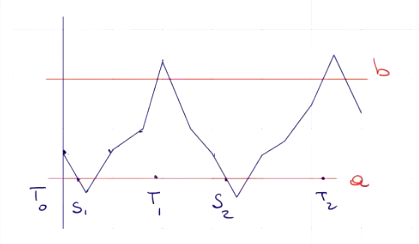
\includegraphics[width=0.62\linewidth]{screenshot016}
	\caption{Up and downs. Just like my consumption of cocaine and my mood respectively on an average tuesday evening.}
	\label{fig:screenshot016}
\end{figure}
We call $S_{k}$\emph{ downcorssing time} while we call $T_{k}$ \emph{upcrossing time}. \\
Now consider the sequence $(T_0,S_1,T_1,S_2,T_2,\ldots)$. It is an increasing sequence of stopping times. If we want to focus on the number of oscillations we may count how many times we go from an upcrossing to a downcrossing time (or vice-versa). Say we want to count the upcrossing. We can define a quantity
\begin{equation*}
	U_{n}(a,b)=\sum_{k=1}^{\infty}\indi_{(0,n]}(T_{k})
\end{equation*}
which of course is a counting process.
\begin{example}
	We are still with our financebros. Suppose that $(M_{n})$ is the price of an asset at time $n$. We want to buy when the price is below $a$ at time $S_i$ and sell when it is above $b$ at time $T_i$. In $(0,n]$ we have $U_{n}(a,b)$ cycles of buying and selling so our strategy could consists in holding a number $F_{n}$ of shares during period $(m-1,m]$. This means introducing
	\[F_{m}=\sum_{k=1}^{\infty}\indi_{(S_{k},T_{k}]}\]
	with $F_{0}=0$. We can thus trace the evolution of our capital with the discrete-time integral:
	\[X=\int F\dif M\]
	And the profit during $(0,n]$will be $X-X_{0}$.\\
	The profit is at least
	\begin{equation*}
		(b-a)U_{n}(a,b).
	\end{equation*}
\end{example}
\begin{proposition}
	If $M$ is a sub-martingale with respect to its natural filtration then 
	\begin{equation*}
		(b-a)\ev U_{n}(a,b)\leq\ev\left[(M_{n}-a)^{+}-(M_{0}-a)^{+}\right].
	\end{equation*}
\end{proposition}
We wanted to find a bound for our profit, but our profit is a stochastic quantity: so it's only natural to think about the expectation to give a bound to the number of expected up/downcrossing.\\
Observe that the number of upcrossings does not depend on the value of $T_0$ that we fix.
\begin{fancyproof}
	Choose $a=0$. Consider hence the process $(M-a)^{+}$ that is sub-martingale (if $M$ is a sub-martingale). Take $M\geq 0$ and let 
	\begin{equation*}
		F_{n}-\sum_{k=1}^{\infty}\indi_{(S_{k},T_{k}]}(n)
	\end{equation*}
	and consider 
	\begin{equation*}
		X=\int F\dif M
	\end{equation*}
	like in our example. We know that $F$ is predictable since by definition $F_{k+1}\in\F_{k}$. Consider the expectation of the increment
	\begin{equation*}
		\ev[X_{k+1}-X_{k}|\F_{k}]=\ev\left[F_{k+1}(M_{k+1}-M_{k})|\F_{k}\right].
	\end{equation*}
	But since $F_{k+1}$ is predictable we can take it out the expectation:
	\begin{equation*}
		F_{k+1}\ev\left[M_{k+1}-M_{k}|\F_{k}\right].
	\end{equation*}
	But since $F_{k+1}$ is an indicator we know it is $\leq1$:
	\begin{equation*}
			\ev[X_{k+1}-X_{k}|\F_{k}]\leq\ev\left[M_{k+1}-M_{k}|\F_{k}\right].
	\end{equation*}
	Now take the expectation of both sides:
	\begin{equation*}
		\ev[X_{k+1}-X_{k}]\leq\ev\left[M_{k+1}-M_{k}\right].
	\end{equation*}
	If we sum these inequalities over $k$ we get:
	\begin{equation*}
		\ev\left[X_{n}-X_{0}\right]\leq\ev\left[M_{n}-M_{0}\right].
	\end{equation*}
	So we now get that
	\begin{equation*}
		bU_{n}(a,n)\leq\ev\left[X_{n}-X_{0}\right]\leq\ev\left[M_{n}-M_{0}\right]
	\end{equation*}
	but given that $a=0$ we get that
	\begin{equation*}
		bU_{n}(0,b)\leq\ev[M_{n}-M_{0}].
	\end{equation*}
	Clearly we have to take the positive part.
\end{fancyproof}
This characterizes our martingale and its boundedness. The number of oscillations of a sub-martingale is bounded! The next question is: can we say anything about the behaviour of maximum/minimum of a martingale or sub-martingale? 
\begin{remark}
	Consider a sequence $\{X_{n}\}$ of independent \rv s with $\ev X_{n}=0,S_n=\sum X_{i}$. We proved that
	\begin{equation*}
		a^{2}\pr(\max_{k\leq n}|S_{k}|>a)\leq\var S_{n}
	\end{equation*}
	and we called this \emph{Kolmogorov's inequality}.
\end{remark}
What we are doing here is considering a random walk whose jumps have 0 mean. We wonder wether it is above the level $a$ as seen in figure \ref{fig:screenshot017}.
\begin{figure}[h]
	\centering
	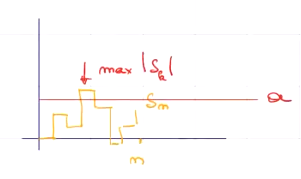
\includegraphics[width=0.6\linewidth]{screenshot017}
	\caption{The maximum of the random walk.}
	\label{fig:screenshot017}
\end{figure}
About this, we know that $\{S_{n}\}$ is a $\F$-martingale but in proving the Kolmogorov's inequaility we never talked about the martingale property! We could improve this inequality using the \emph{Doob's martingale inequality}. The problem is that we can prove very general inequalities that hold true for any \rv s but specifying more characteristic we can obtain stricter bounds. In this framework let's define 
\begin{equation*}
	\begin{array}{l}
		M^{\star}_{n}=\max_{k\leq n}M_{k}\\
		m^{\star}_{n}=\min_{k\leq n}M_{k}\\
	\end{array}
\end{equation*}
as current maximum and current minimum of $M$.
\begin{theorem}
	Take $M$ as a sub-martingale. For $b>0$ it holds:
	\begin{enumerate}
		\item $b\pr(M^{\star}_{n}\geq b)\leq\ev\left[M_{n}\indi_{\{M_{n}^{\star}\geq b\}}\right]\leq\ev\left[M_{n}^{+}\right]$;
		\item $b\pr(m^{\star}_{n}\leq-b)\leq-\ev M_{0}+\ev\left[M_{n}\indi_{\{m_{n}^{\star}\geq b\}}\right]\leq\ev M_{n}^{+}-\ev M_{0}$.
	\end{enumerate}
\end{theorem}
So we can further bound the result looking into the property of $M_{n}$.
\begin{example}
	Prof. Sacerdote fucked up so we now need to define the brownian motion (or Weiner process).
	\begin{definition}
		A real-valued stochastic process $B={(B_{t})}_{t\geq0}$ is called \emph{brownian motion} if:
		\begin{enumerate}
			\item the index set is $\R^{+}$;
			\item $B_{0}(\omega)=0$ for almost all $\omega$;
			\item $B_{t_{n}}-B_{t_{n-1}},\ldots,B_{t_{1}}-B_{t_{0}}$ are independent for $\every 0=t_{0}<t_1<\ldots<t_n<\infty$;
			\item $B_{t}-B_{s}\sim B_{t+b}-B_{s+b}$ for every $0\leq s<t<\infty\quad\every n>- s$;
			\item $B_{t}-B_{s}\sim N(0,t-s)$;
			\item $t\mapsto B_{t}(\omega)$ are continuous for every $\omega$.
		\end{enumerate}
	\end{definition}
	The brownian motion is in itself a martingale, but there is a class of martingales strictly related to it:
	\begin{equation*}
		M_{t}=\exp\left\{\lambda B_{t}-\frac{1}{2}\lambda^{2}t\right\},\qquad t\in\R^{+}.
	\end{equation*}
	Now we can get to the actual example: if $B$ is a brownian motion, we have 
	\begin{equation*}
		\pr(\sup_{0\leq t\leq\theta}B_{t}\geq b)\leq\exp\left\{-\frac{b^{2}}{s\theta}\right\}.
	\end{equation*}
	The sample paths of brownian motions are extremely irregular. We are asking with which probability the max of our process will be over $b$ at time $\theta$.
	\begin{figure}[H]
		\centering
		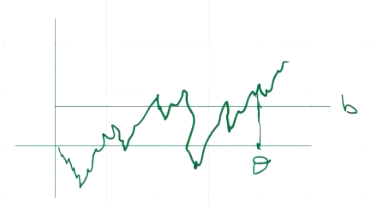
\includegraphics[width=0.6\linewidth]{screenshot018}
		\caption{Check out Autechre. A staple in electronic experimental music.}
		\label{fig:screenshot018}
	\end{figure}
	I am basically asking if the maximum attained is above or below $b$.
	How can we use the Doob's inequality?
	\begin{fancyproof}
		Consider
		\begin{equation*}
			\pr(\sup B_{t}\geq b)=\pr(\sup e^{\lambda B_{t}}\geq e^{\lambda b})
		\end{equation*}
		and using Doob's inequality
		\begin{align*}
				\pr(\sup B_{t}\geq b)&=\pr(\sup e^{\lambda B_{t}}\geq e^{\lambda b})\\
				&\leq \frac{\overbrace{\ev\left[e^{\lambda B_{\theta}-\frac{\lambda^{2}}{2}\theta}\right]}^{\text{martingale}}}{e^{\lambda b}e^{-\frac{\lambda^{2}}{2}\theta}}\\
				&=e^{-\lambda b+\frac{\lambda^{2}}{2}\theta}\qquad\every\lambda>0
			\end{align*}
	\end{fancyproof}
\end{example}
Now we have to prove Doob's inequality.
\begin{fancyproof}
	We introduce 2 stopping times: 
	\begin{equation*}
		\begin{array}{l l}
			T&=\inf\{n\geq0:M_{n}\geq b\}\\
			S&=\inf\{n\geq0:M_{n}\leq-b\}.
		\end{array}
	\end{equation*}
	\begin{figure}[H]
		\centering
		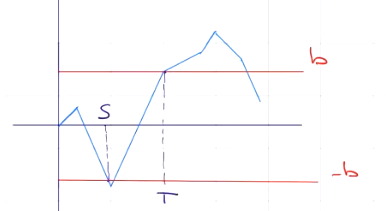
\includegraphics[width=0.6\linewidth]{screenshot019}
		\caption{Also Aphex Twin. Really, Autechre and Aphex Twin are probably the best example of the boom of experimentation in popular electronic music between 1995 and 2005.}
		\label{fig:screenshot019}
	\end{figure}
	Consider the current maximum and minimum above the level $b$:
	\begin{equation*}
		\{M^{\star}_{n}\geq b\}=\{T\leq n\}\qquad	\{m^{\star}_{n}<-b\}=\{S\leq n\}.
	\end{equation*}
	Fix $b$ and $n$. When $\{T\leq n\}$ we have
	\begin{align*}
		M_{T\wedge n}=M_{T}\geq b.
	\end{align*}
	Multiply by $\indi_{\{T\leq n\}}$:
	\begin{equation*}
		b\indi_{\{T\leq n\}}\leq M_{T\wedge m}\indi_{\{T\leq n\}}.
	\end{equation*}
	Using Doob's stopping theorem we know that 
	\begin{equation*}
		\ev\left[M_{T}-M_{S}|\F_{S}\right]\geq0
	\end{equation*}
	and using $S=T\wedge n$ and $T=n$ we obtain
	\begin{equation*}
		\ev\left[M_{n}|\F_{T\wedge n}\right]>M_{T\wedge n}.
	\end{equation*}
	So summing it all up:
	\begin{align*}
		b\indi_{\{T\leq n\}}&\leq M_{T\wedge m}\indi_{\{T\leq n\}}\\
		&\leq\indi_{\{T\leq n\}}\ev\left[M_{n}|\F_{T\wedge n}\right]\\
		&\ev\left[M_{n}\indi_{\{T\leq n\}}|\F_{T\wedge n}\right].
	\end{align*}
	Now take the expectation:
	\begin{align*}
		b\pr(T\leq n)&=b\pr(M^{\star}_{n}\geq b)\\
		&\leq\underbrace{\ev\left[M_{n}\indi_{\{T\leq n\}}\right]}_{\mathclap{\ev\left[M_{n}\indi_{\{M_{n}^{\star}\geq b\}}\right]}}\\
		&\leq\ev(M^{+}_{n}).
	\end{align*}
	For the minimum we work on $\{S\leq n\}$ and we get 
	\begin{align*}
		M_{S\wedge n}&=M_{S}\indi_{\{S\leq n\}}+M_{S}\indi_{\{S>n\}}\\
		&\leq-b\indi_{\{S\leq n\}}+M_{n}\indi_{S\geq n}.
	\end{align*}
	Now take the expectation:
	\begin{equation*}
		\ev M_{S\wedge n}\leq-b\pr(m^{\star}_{n}\leq-b)+\ev\left[M_{n}\indi_{\{S>n\}}\right].
	\end{equation*}
	So that we get
	\begin{equation*}
		\pr(m^{\star}_{n}\leq-b)\leq-\ev M_{S\wedge n}+\ev[M_{n}\indi_{\{S>n\}}].
	\end{equation*}
	Now use Doob's stopping theorem with $T=0$ and $S=S\wedge n$ so that $\ev M_{0}\leq\ev M_{\{S\wedge n\}}$. This gets us our result:
	\begin{align*}
		b\pr(m^{\star}_{n}-b)&\leq-\ev M_{0}+\ev\left[M_{n}\indi_{\{m_{n}^{\star}\}}\right]\\
		&\leq\ev M^{+}_{n}-\ev M_{0}.
	\end{align*}
\end{fancyproof}
\begin{remark}
	If $M$ is a martingale then $|M|^{p}$ is a sub-martingale for $p\geq1$. If $M_{n}\in\lp\every n$ we can apply Doob's inequality.
\end{remark}
\begin{corollary}
	If $M$ is martingale in $\lp$ for some $p\geq 1$ then for $b>0$ we have that
	\begin{equation*}
		b^{p}\pr(\max_{k\leq n}|M_{k}|>b)\leq\ev|M_{n}|^{p}.
	\end{equation*}
\end{corollary}
There are also other bounds:
\begin{itemize}
	\item $b\pr(\max_{k\leq n}|M_{k}>b)\leq 2\ev M_{n}^{+}-3M_{0}$;
	\item \emph{Doob's norm inequality}: if $M$ is a martingale in $\lp,p\geq 1$ and $q$ is the exponent conjugate to $p$ ($\frac{1}{p}+\frac{1}{q}=1$) then
	\begin{equation*}
		\ev\max_{  k\leq n}|M_{k}|^{p}\leq q^{p}\ev|M_{n}|^{p}.
	\end{equation*}
	\item  Consider $L^{2}$-bounded martingales characterized by final coordinate $X$ with $\var X=\sigma^{2}$ (that is I am fixing the variance of the last value I consider). We want to assess the variability of this process.
	\begin{theorem}
		\emph{Dubin \& Schwartz 1998}: it holds
		\begin{enumerate}
			\item $\ev\left[\max_{0\leq T\leq t}M_{T}\right]\leq\sigma$;
			\item $\ev\left[\max_{0\leq T\leq t}|M_{T}|\right]\leq\sigma\sqrt{2}$.
		\end{enumerate}
		Moreover, there exist suitable martingales for which this bound is attained and is scrict.
	\end{theorem}
\end{itemize}
\subsection{Limit of sequences of \rv s}
Consider a sequence of \rv s $\{X_{n}\}$ with independence between the \rv. Then we know that if $\lim X_{n}$ exists then the limit is a constant. Why?
\begin{remark}
	If the $\lim_{n}X_{n}$ exists than it belongs to the tail \sa{} $\tau$. Since the \rv s are independent then we can apply the 0-1 Kolmogorov law, so the probability that the \rv{} is infinity is either 0 or 1 but if this is the case then it must be a constant.
\end{remark}
This is about the behavior in the limits of a sequence of \rv s with independence between $\{X_{n}\}$. Then if the limit exists it is a constant, since $\lim_{n}X_{n}$ belongs to the tail \sa{} of the sequence. Independency between \rv s tells us that we can apply Kolmogorov's 0-1 law to say that $\pr(\lim_{n}X_{n}=\infty)$ is either 0 or 1... but if we somehow know that the limit exists then it can't be $\infty$ so its probability of being $\infty$ is 0 and therefore it is a constant almost surely! This is cool because it tells us that the limit is either infinite or finite.
If $\{X_{n}\}$ is a submartingale consider the limit 
\begin{equation*}
	\lim_{n\to\infty}X_{n}=X_{\infty}
\end{equation*}
What the fuck? What is this object? Consider the case in which $\T=\N$. We know that the expected value $\{\ev X_{n}\}$ is an increasing sequence if the process is a sub-martingale. 
We have our first theorem about convergence:
\begin{theorem}
	Let $X$ be a sub-martingale. If (and note that is a sufficient condition)
	\begin{equation*}
		\sup_{n}\ev X_{n}^{+}<\infty
	\end{equation*}
	Then
	\begin{enumerate}
		\item $\{X_{n}\}$ converges $\as$;
		\item $\{X_{n}\}$ converges to an integrable \rv.
	\end{enumerate}
\end{theorem}
Before proving think about it. \begin{enumerate}
\item	The condition of this theorem requires that $X^{+}$ is in $L^{1}$ and is bounded. If $X$ is a sub-martingale then also $X^{+}$ is a sub-martingale... But this means that $\ev X^{+}_{n}$ is an increasing sequence. Our condition gives a bound to the increase of this sequence! But this means that I am trying to avoid the divergence of the expected value (which means: trying to control the rate of our martingale). 
\item Now think about a negative sub-martingale: this would verify the condition so there is no problem about it.
\item Now think about a positive super-martingale: it is only a negative sub-martingale with another sign so it converges.
\item Consider now a positive or bounded martingale or a negative martingale. All of these cases converge. 
\item $\sup\ev X_{n}^{+}<\infty\iff\sup\ev|X_{n}|\leq\infty$. Let $\{X_{n}\}$ be a sub-martingale such that
\begin{equation*}
	\ev X_{n}>\ev X_{0}\qquad\every n.
\end{equation*}
But now \begin{equation*}
	\ev|X_{n}|=\ev X_{n}^{+}-\ev X_{n}^{-}=\ev X_{n}^{+}+\ev_{n}^{+}-\ev X_{n}
\end{equation*}
So
\begin{align*}
	\ev X_{n}^{+}&\leq\ev|X_{n}|=2\ev X_{n}^{+}-\ev X_{n}\\
	&\leq 2\underbrace{\ev X_{n}^{+}}_{<\infty}-\ev X_{0}\leq\infty
\end{align*}
So $\ev|X_{n}|\leq\infty$.
\end{enumerate}
\begin{fancyproof}
	We prove the theorem by contradiction. Pick an outcome $\omega$ and suppose that $\{X_{n}(\omega)\}$ is a numerical sequence that has not a limit. But if it doesn't have a limit, then 
	\[\exists\inf\lim\neq\sup\lim\qquad\inf\lim<\sup\lim.\]
	So there exist at least 2 rationals $a<b$ such that
	\begin{equation*}
		\inf\lim<a<b<\sup\lim.
	\end{equation*}
	The sequence $\{X_{n}(\omega)\}$ crosses $(a,b)$ $\infty$ many times. Now take the union over rational $a$ and $b$, $a<b$ of the sets
	\begin{equation*}
		\{U(a,b)=\infty\}
	\end{equation*}
	with $U(a,b)=\lim_{n\to\infty}U_{n}(a,b)$. Our aim is now to show that $U(a,b)\leq\infty$ almost surely to get a contradiction.\\
	Fix $a,b$. We know that $U_{n}(a,b)$ is increasing with $n$. Now consider
	\begin{align*}
		(b-a)\ev U(a,b)&=(b-a)\ev\lim U_{n}(a,b)\\
		&\underset{\mathclap{\text{monotone conv.}}}{=}(b-a)\lim\ev U_{n}(a,b)\\
		&\underset{\mathclap{\text{upcross inequalities}}}{\leq}\sup\ev(X_n-a)^{+}\\
		&\leq \sup\ev X_{n}^{+}+|a|.
	\end{align*}
	So this means that $\ev U(a,b)<\infty$. But this is a contradiction, so it exists a limit $X_{n}=X_{\infty}\as$.\\
	Now consider the second part of the theorem:
	\begin{align*}
		\ev|X_{\infty}|&=\ev\lim\inf|X_{n}|\\
		&\underset{\mathclap{\text{Fatou's lemma}}}{\leq}\lim\inf\ev|X_{n}|\\
		&\leq 2\sup\ev X_{n}^{+}-\ev X_{0}\leq\infty
	\end{align*}
	so the limit is integrable.
\end{fancyproof}
Here everything is related to integrability conditions but this is a sufficient condition. What if we want a sufficient and necessary condition? Well, consider $\sup_n\ev X_{n}^{+}\leq\infty$. We want to control the tail uniformly not only on the tail but on the whole process.
\begin{figure}[h]
	\centering
	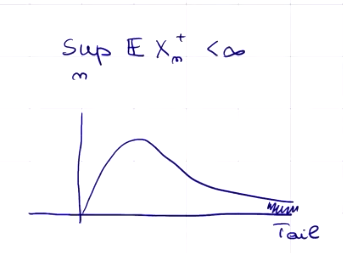
\includegraphics[width=0.6\linewidth]{screenshot020}
	\caption{It's astonishing how much a bad teacher can have you hate a subject.}
	\label{fig:screenshot020}
\end{figure}
We recall that we already introduced a strong condition for uniform integrability. w
We will need:
\begin{enumerate}
	\item a collection $\mathcal{K}$ of real \rv s is said to be uniformly integrable if 
	\begin{equation*}
		k(b)=\sup_{X\in\mathcal{K}}\ev|X|\indi_{\{X>b\}}\xrightarrow[b\to\infty]{}0.
	\end{equation*}
	\item If $\mathcal{K}$ is dominated by an integrable \rv{} $Z$ then it is uniformly integrable.
	\item uniform integrability implies $L^{1}$-boundedness but not the converse.
	\item If $\mathcal{K}$ is $L^{p}$-bounded for some $p>1$ then it is uniformly integrable.
\end{enumerate}
\begin{lemma}
	Let $Z$ be an integrable \rv{}. Then
	\begin{equation*}
		\mathcal{K}=\left\{X:X=\ev(Z|\G)\right\}
	\end{equation*}
	for some sub-\sa{} $\G$ of $\HS$ is uniformly integrable.
\end{lemma}
\begin{proposition}
	Let $Z$ be an integrable \rv{}. Define 
	\begin{equation*}
		X_{t}=\ev(Z|\F_{t})\qquad t\in\T.
	\end{equation*}
	This means that $\{X_{t}\}$ is a uniformly integrable $\F$-martingale.
\end{proposition}
\begin{theorem}
	Let $\{X_{n}\}$ be a sequence of real-valued \rv s. The following are equivalent:
	\begin{enumerate}
		\item it converges in $L^{1}$;
		\item it converges in probability and it is uniformly integrable.
	\end{enumerate}
\end{theorem}
We can now prove the theorem about the convergence of sub-martingales.
\begin{theorem}
	Let $X$ be a sub-martingale. We have that $X$ converges almost surely and in $L^{1}$ \ifonly{} it is uniformly integrable. Moreover, if it is so, setting 
	\begin{equation*}
		X_{\infty}=\lim X_{n}
	\end{equation*}
	extends $X$ to a sub-martingale
	\begin{equation*}
		\xbar={(X_{n})}_{n\in\overline{\N}}.
	\end{equation*}
\end{theorem}
We only prove the first part of the theorem.
\begin{fancyproof}
	\emph{Necessity}. If $X$ converges in $L^{1}$ by the theorem above it is uniformly integrable.\\
	\emph{Sufficiency}. If $X$ is uniformly integral then it is $L^{1}$-bounded for the property above. So our previous theorem holds and the martingale converges almost surely with $X_{\infty}$ integrable. Furthermore, for the property above, it also converges in $L^{1}$.
\end{fancyproof}
Is there a way to get a uniformly integrable sub-martingale?
\begin{theorem}
	A process $M={(M_{n})}_{n\in\N}$ is a uniformly integrable martingale \ifonly{} for some integrable \rv{} $Z$
	\begin{equation}
		M_{n}=\ev\left[Z|\F_{n}\right]\qquad n\in\N.\tag{$\bullet$}\label{AAAA}
	\end{equation}
	If so it converges almost surely and in $L^{1}$ to the integrable \rv
	\begin{equation*}
		M_{\infty}=\ev[Z|\F_{\infty}].
	\end{equation*}
\end{theorem}
\begin{corollary}
	For every integrable \rv{} $Z$ we have
	\begin{equation*}
		\ev(Z|\F_{n})\convas\xrightarrow[]{L^{1}}\ev(Z|\F_{\infty}).
	\end{equation*}
\end{corollary}
\begin{theorem}
	Let $Z$ be an integrable \rv{} and let 
	\begin{equation*}
		M_{n}=\ev(Z|\F_{n})_{n\in\overline{\N}}.
	\end{equation*}
	For every stopping time $T$ define
	\begin{equation*}
		M_{T}=\ev[Z|\F_{T}]
	\end{equation*}
	and for arbitrary stopping times $S$ and $T$ we get
	\begin{equation*}
		\ev[M_{T}|\F_{S}]=M_{S\wedge T}.
	\end{equation*}
\end{theorem}
This lets us rethink Doob's theorem.
\begin{theorem}
	If $S$ and $T$ are arbitrary stopping times such that $S\leq T$ then
	\begin{equation*}
		\ev[M_{T}|\F_{S}]=M_{S}
	\end{equation*}
	for an uniformly integrable martingale.
\end{theorem}
The dominated convergence theorem requires adaptness. 
\begin{theorem}
	\emph{Hunt's dominated convergence theorem}.\\
	Let $\{X_{n}\}$ be dominated by an integrable \rv{} and suppose that exists
	\begin{equation*}
		X_{\infty}=\lim X_{n}
	\end{equation*}
	So ${(\ev_{n}X_{n})}_{n}$ converges to $\ev X_{\infty}$ almost surely and in $L^{1}$.
\end{theorem}
To prove we should use Borel-cantelli somehow.
\chapter{Exercises and questions}
\section{Exercises with Prof. Issoglio (2024/2025)}
\subsection{Exercise class 1}
\begin{exercise}
	Consider the experiment where we throw a coin infinitely many times, so that 
	\begin{equation*}
		\Omega=\{H,T\}^{\N} \qquad\text{(or $\{0,1\}^{\N}$)}.
	\end{equation*}
	In particular, the event $\omega\in\Omega$ is of the form $\omega=(\omega_1,\omega_2,\ldots)$ with $\omega_i\in\{0,1\}$. Let 
	\begin{equation*}
		C:=\left\{\left\{\omega\in\Omega:\omega_k=a,a\in\{0,1\},n\in\N\right\}\right\}
	\end{equation*}
	and 
	\begin{equation*}
		\F:=\sigma(C).
	\end{equation*}
	We want to check whether $\F$ is a good modeling choice for our experiment. For example, if we set
	\begin{equation*}
		A:=\left\{..\right\}
	\end{equation*}
\end{exercise}

\subsection{Exercise class 2}
\subsection{Exercise class 3}
\subsection{Exercise class 4}
\subsection{Exercise class 5}
\subsection{Exercise class 6}
\subsection{Exercise class 7}
\subsection{Exercise class 8}
\section{Questions for the oral examination}
Here I will try and answer to the questions that were on the moodle site about the year 2022-2023. I hope that they will be valid for the years to come as well.
\subsection{Transition kernels: definition, example, and their usage in the extension of measures to
product spaces}
First of all, the definition:
\begin{definition}
	Let $(E,\E)$ and $(F,\F)$ be measurable spaces. Let $K$ be a mapping from $E\times\F$ into $\overline{\R}_+$. Then $K$ is called \emph{transition kernel} from space $(E,\E)$ into space $(F,\F)$ if:
	\begin{itemize}
		\item the mapping $x\mapsto K(x,B)$ is $\E$-measurable $\every B\in\F$;
		\item the mapping $B\mapsto K(x,B)$ (the second mapping of the kernel, the one regarding the set) is a measure $\every x\in E$.
	\end{itemize}
\end{definition}
Then the example:
\begin{example}
	Take $\nu$, a finite measure on $(F,\F)$ and take $k$, a positive function on $(E\times F)$ which is measurable with respect to $\E\otimes\F$, the product \sa{}. Then, we integrate
	\[\int_B\nu(\dy)k(x,y)\qquad\begin{array}{l}
		B\in\F\\
		x\in E
	\end{array}\]
	We see how this object depends on $x$ and on the choice of $B$ (a function of $x$ and $B$...). It defines a transition kernel
	\[K(x,B)=\int_B\nu(\dy)k(x,y)\qquad\begin{array}{l}
		B\in\F\\
		x\in E
	\end{array}\]
	from $(E,\E)$ into $(F,|F)$.
\end{example}
Now the extensions of measures on product spaces;
\begin{theorem}
		\emph{Extension of measures on product spaces}.\\
	Let $\mu$ be a measure on the measurable space $(E,\E)$. Let $K$ be a $\Sigma$-finite\footnote{Erm... what the sigma?} transition kernel from space $(E,\E)$ into $(F,\F)$. Then:
	\begin{enumerate}[\circnum]
		\item if we take our function $f(x,y)$, integrate it against our kernel $K(x,\dx)$ over $F$ and then integrate again against measure $\mu$ over $E$, the operation 
		\[\pi f=\int_E\mu(\dx)\int_FK(x,\dy)f(x,y)\]
		defines a measure $\pi$ on $(E\times F,\E\otimes\F)$;
		\item if $\mu$ is $\sigma$-finite and $K$ is $\sigma$-bounded then $\pi$ is $\sigma$-finite and it is the unique measure on $(E\times F,\E\otimes\F)$ satisfying
		\[\pi(A\times B)=\int_A\mu(\dx)K(x,B)\qquad\every A\in\E,B,\in\F.\]
	\end{enumerate}
\end{theorem}
\subsection{Kolmogorov’s 0-1 law: proof and an example of its usage}
First, the statemente of the theorem.
\begin{theorem}
	\emph{Kolmogorov's 0-1 law}\\
	This is a theorem about independence. Let $\G_1,\G_2,\ldots$ be independent. Then
	\[\pr(H)=\begin{cases}
		0\\
		1
	\end{cases}\qquad\every H\in\tau.\]
\end{theorem}
and here's the short proof:
\begin{fancyproof}
	Start from your independency $(\G_1,\G_2,\ldots)$, then put the last $\G$'s in a partition (which is still an independency) $(\G_1,\G_2,\ldots,\G_n,\tau_n)$. Now consider that the tail \sa{} is a subset of $\tau_n$ and this means that $(\G_1,\G_2,\ldots,\G_n,\tau)$ is still an independency... But we also know that this is true for every $n$ up to $\infty$ and so we can extend the independency to a collection of countably many partitions, since ${(\G_1,\G_2,\ldots,\G_n,\tau)}_{n}$ us a countably infinite sequence of independencies. So
	\begin{equation*}
		(\tau,\G_1,\G_2,\ldots)
	\end{equation*}
	is an independency. Do another partition (which still gives us an independency) and get the independency
	\begin{equation*}
		(\tau,\tau_0)
	\end{equation*}
	but then remember that $\tau_0$ is an \textit{union} of the \sa s from 1 to $\infty$ while $\tau$ is an \textit{intersection} of all $\tau_n$ including $\tau_0$, so we have that $\tau\subset\tau_0$.\\
	Consider now $\pr(H\cap G)$ where $H\in\tau$ and $G\in\tau_0$. Due do independency we have that 
	\begin{equation*}
		\pr(H\cap G)=\pr(H)\pr(G)
	\end{equation*}but since all elements of $\tau$ are also elements of $\tau_0$ we can choose $G\equiv H$ and our equation becomes
	\begin{equation*}
		\pr(H\cap G)=\pr(H\cap H)=\pr(H)=\pr(H)^{2}
	\end{equation*}
	and the solution to this can only be 0 or 1.
\end{fancyproof}
We still need an example of the application... that would be, for example, the behavior in the limits of a sequence of \rv s with independence between $\{X_{n}\}$. Then if the limit exists it is a constant, since $\lim_{n}X_{n}$ belongs to the tail \sa{} of the sequence. Independency between \rv s tells us that we can apply Kolmogorov's 0-1 law to say that $\pr(\lim_{n}X_{n}=\infty)$ is either 0 or 1... but if we somehow know that the limit exists then it can't be $\infty$ so its probability of being $\infty$ is 0 and therefore it is a constant almost surely! This is cool because it tells us that the limit is either infinite or finite. This is useful for sub-martingales. 
\subsection{Almost sure convergence: definition, properties and characterization theorem}
Start with the definition:
\begin{definition}
	A real-valued sequence of \rv s ${(X_n)}_{n}$ on $(\Omega,\HS,\pr)$ is said to be \emph{almost sure convergent} (a.s. convergent) is the numerical sequence
	\[{\Big(X_n(\omega)\Big)}_{n}\]
	converges for almost all $\omega\in\Omega$. \\
	It is said to converge to $X$ if $X$ is an almost sure real-valued \rv{} and 
	\[\lim_{n\to\infty}X_n(\omega)=X(\omega)\]
	for almost all $\omega\in\Omega$.
\end{definition}
The characterization is
\begin{theorem}
	\emph{Characterization of almost sure convergence}:\\
	A sequence of real valued \rv s ${(X_n)}_{n}$ converges to $X$ almost surely \ifonly{}, for every $\varepsilon>0$,
	\begin{equation*}
		\sum_n\mathcal{i}_\varepsilon\circ|X_n-X|<\infty
	\end{equation*}
	almost surely.
\end{theorem} Where $\mathcal{i}_\varepsilon$  is the indicator function of $(\varepsilon,\infty)$:
\[\mathcal{i}_\varepsilon(x)=\indi_{(\varepsilon,\infty)}(x)=\begin{cases}
1, &x>\varepsilon\\
0, &x\leq \varepsilon.
\end{cases}\]
This basically means that in every interval from a certain point $\varepsilon$ to $\infty$ the sum of the differences of $X_n$ and $X$ must not diverge. Here are some properties:
\begin{itemize}
	\item \textbf{Comparison with Other Types of Convergence:}
	\begin{itemize}
		\item If $\{X_n\}$ converges almost surely to $X$, then $\{X_n\}$ also converges to $X$ in probability.
		\item Almost sure convergence implies convergence in distribution, but not necessarily vice versa.
	\end{itemize}
	
	\item \textbf{Closure Under Linear Operations:}
	\begin{itemize}
		\item \textbf{Addition:} If $X_n \to X$ a.s. and $Y_n \to Y$ a.s., then $X_n + Y_n \to X + Y$ a.s.
		\item \textbf{Multiplication:} If $X_n \to X$ a.s. and $Y_n \to Y$ a.s., then $X_n Y_n \to XY$ a.s. (provided $X$ and $Y$ are bounded or measurable in a compatible way).
	\end{itemize}
	
	\item \textbf{Countable Additivity:}
	\begin{itemize}
		\item \textbf{Countable Unions:} If $\{X_n\}$ converges almost surely to $X$, then for any countable collection of events $\{A_i\}$ with $\Pr(A_i) \to 0$, $\Pr(\limsup_{i \to \infty} A_i) = 0$.
	\end{itemize}
	
	\item \textbf{Uniform Integrability:}
	\begin{itemize}
		\item \textbf{Expectation Convergence:} If $\{X_n\}$ converges almost surely to $X$ and $\{X_n\}$ is uniformly integrable, then $X_n \to X$ in $L^1$, meaning $\mathbb{E}[|X_n - X|] \to 0$.
	\end{itemize}
	
	\item \textbf{Continuity from Below and Above:}
	\begin{itemize}
		\item \textbf{From Below:} If $X_n \leq X_{n+1}$ a.s. for all $n$ and $X_n \to X$ a.s., then $X_n \leq X$ a.s.
		\item \textbf{From Above:} If $X_n \geq X_{n+1}$ a.s. for all $n$ and $X_n \to X$ a.s., then $X_n \geq X$ a.s.
	\end{itemize}
	
	\item \textbf{Interchange of Limits:}
	\begin{itemize}
		\item \textbf{Expectation Limit:} If $X_n \to X$ a.s. and $\{X_n\}$ is uniformly integrable, then $\mathbb{E}[X_n] \to \mathbb{E}[X]$.
	\end{itemize}
	
	\item \textbf{Fatou's Lemma and Monotone Convergence Theorem:}
	\begin{itemize}
		\item \textbf{Fatou’s Lemma:} If $X_n \geq 0$ almost surely and $X_n \to X$ a.s., then $\mathbb{E}[X] \leq \liminf_{n \to \infty} \mathbb{E}[X_n]$.
		\item \textbf{Monotone Convergence Theorem (for non-negative random variables):} If $X_n \to X$ a.s. and $X_n \geq 0$ a.s., then $\mathbb{E}[X] = \lim_{n \to \infty} \mathbb{E}[X_n]$.
	\end{itemize}
\end{itemize}
\subsection{Borel Cantelli lemmas; proof of the divergence part}
Enunciate the two lemmas side by side (and with a slightly different formulation).
\begin{theorem}
	\emph{Borel-Cantelli lemmas}\\
	\begin{enumerate}[a)]
		\item Let ${(B_n)}_{n}$ be a sequence of Bernoulli \rv s.
		\[\sum_n \ev B_n<+\infty\implies\sum_n B_n<+\infty\as\]
		\item If 
		\[\sum_n\ev B_n=\infty\text{ and }{(B_n)}_{n}\text{ are pairwise independent}\]
		then
		\[\sum_n B_n=+\infty\as\]
	\end{enumerate}
\end{theorem}
Now let's prove the divergent part.
	\begin{notation}
	\[p_n=\ev B_n,\quad a_n=\sum_{i=1}^n\ev B_i=\sum_{i=1}^{n}p_i\]
	and we get the partial sum and the limits
	\[S_n=\sum_{i=1}^{n}B_i,\quad S=\lim_n S_n\]
\end{notation}
\begin{fancyproof}
	Ok, this is long. We know that, since the \rv s are pairwise independent,
	\begin{equation*}
		\var S_{n}=\sum_{i=1}^{n} \var B_{n}=\sum_{i=1}^{n} p_{n}(1-p_{n})\leq\sum_{i=1}^{n}p_n=a_{n}.
	\end{equation*}
	Then fix $b\in(0,\infty)$. Since we know that ${(a_{n})}_{n}$ is increasing towards $\infty$ then the same can be said of 
	\begin{equation*}
		{\left(a_{n}-\sqrt{ba_{n}}\right)}_{n}
	\end{equation*}
	since we are subtracting to $a_{n}$ a quantity that goes towards $\infty$ more slowly. So the sequence still goes towards infinity and this means that the event ${S<\infty}$ is basically the limit of the increasing sequence of events 
	\[{\left\{S<a_{n}-\sqrt{ba_{n}}\right\}}_{n}.\]
	Since $S_{n\leq S}$ we have that
	\begin{equation*}
		\left\{S<a_{n}-\sqrt{ba_{n}}\right\}\subset\left\{S_{n}<a_{n}-\sqrt{ba_{n}}\right\}
	\end{equation*}
	and we also have that
	\begin{equation*}
		\left\{S_{n}<a_{n}-\sqrt{ba_{n}}\right\}\subset\left\{|S_{n}-a_{n}|>\sqrt{ba_{n}}\right\}
	\end{equation*}
	Since we are dealing with inclusion of events we can look at this from the point of view of probability measures:
	\begin{equation*}
		\pr\left(S<a_{n}-\sqrt{ba_{n}}\right)\leq\pr\left(S_{n}<a_{n}-\sqrt{ba_{n}}\right)\leq\pr\left(|S_{n}-a_{n}|>\sqrt{ba_{n}}\right).
	\end{equation*}
	We take the $\limsup_n$ for two of these probabilities:
	\begin{equation*}
		\limsup_n\left(\pr\left(S<a_{n}-\sqrt{ba_{n}}\right)\right)\leq\limsup_n\left(\pr\left(|S_{n}-a_{n}|>\sqrt{ba_{n}}\right)\right)
	\end{equation*}
	but the first term of this inequality becomes
	\begin{align*}
			\limsup_n\left(\pr\left(S<a_{n}-\sqrt{ba_{n}}\right)\right)&=\pr\left(\lim_{n}\left(\pr\left(S<a_{n}-\sqrt{ba_{n}}\right)\right)\right)\\
			&=\pr\left(S<\infty\right)
	\end{align*}
	since the quantity ${\left\{S<a_{n}-\sqrt{ba_{n}}\right\}}_{n}$ goes towards infinity. Now we can rewrite the previous inequality and use Chebyshev's inequality:
	\begin{align*}
		\pr\left(S<\infty\right)&\leq\limsup_n\left(\pr\left(|S_{n}-a_{n}|>\sqrt{ba_{n}}\right)\right)\\
		&\leq\limsup_n\left(\frac{\var S_{n}}{ba_{n}}\right)\\
		&\leq\limsup_n\left(\frac{\cancel{a_{n}}}{b\cancel{a_{n}}}\right)=\frac{1}{b}.
	\end{align*}
	Since $b$ is arbitrary we can let it go towards infinty and thus obtain that
	\begin{equation*}
		\pr\left(S<\infty\right)\leq0
	\end{equation*}
	But this means that the probability of the complementary event must be 1:
	\begin{equation*}
		\pr\left(S=\infty\right)=1.
	\end{equation*}
\end{fancyproof}
\subsection{Borel Cantelli lemmas; proof of the convergence part, relations with a.s. convergence and
examples of its application}
Start by enunciating the theorem.
\begin{theorem}
	\emph{First Borel-Cantelli Lemma}
	Let ${(H_n)}_{n}$ be a sequence of events. Then
	\[\sum_n\pr(H_n)<+\infty\implies\sum_n\indi_{H_n}<+\infty\quad\text{a.s.}\]
\end{theorem}
The proof is no shit:
\begin{fancyproof}
	Denote $N=\sum\indi_{H_{n}}$ so that $\sum_{n}\pr(H_{n})=\sum_n\ev\indi_{H_{n}}=\ev\sum\indi_{H_{n}}=\ev N$. This means that the new claim is
	\begin{center}
		``If $\ev N<\infty$ then $N<\infty$''
	\end{center}
	But this is true because if the expectation is finite so is its \rv{}. Of course almost surely...
\end{fancyproof}
Now the implications for a.s. convergence:
\begin{proposition}
	Let
	\[\sum_n\pr(|X_n-X|>\varepsilon)<+\infty\qquad\every\varepsilon>0.\]
	Then 
	\[X_n\xrightarrow[]{\text{a.s.}}X.\]
\end{proposition}
\begin{proposition}
	Suppose that there exists a sequence ${(\varepsilon_n)}_{n}$ decreasing to 0 such that
	\[\sum_n\pr(|X_n-X|>\varepsilon_n)<+\infty.\]
	Then
	\[X_n\convas X.\]
\end{proposition}
So we don't need $\varepsilon$ to be constant, but just to be decreasing to 0.
\begin{proposition}
	Suppose that there exists a sequence of positive numbers ${(\varepsilon_n)}_{n}$ such that
	\[\sum_n\varepsilon_n<+\infty,\quad\sum_n\pr(|X_{n+1}-X_n|>\varepsilon_n)<+\infty\]
	Then $X_n$ converges almost surely.
\end{proposition}
\subsection{Convergence in probability: definition, properties and theorem on the metric for
convergence in probability}
Let's start with the definition:
\begin{definition}
	Let ${(X_n)}_{n}$ be a sequence of real-valued random variables. Then ${(X_n)}_{n}$ converges to a further real-valued \rv{} \emph{in probability} if 
	\[\lim_n\pr(|X_n-X|>\varepsilon)=0\qquad\every\varepsilon>0.\]
\end{definition}
I am not sure about properties, why can't you state things clearly? Fuck off. 
\begin{theorem}
	\emph{Characterization theorem for convergence in probability}. 
	\begin{enumerate}[label=\textit{\roman*})]
		\item \label{ehehe} if ${(X_n)}_{n}$ converges to $X$ almost surely, then it converges to $X$ in probability;
		\item \label{ehehe2} if ${(X_n)}_{n}$ converges in probability to $X$, then it has a subsequence converging to the same \rv{} $X$ almost surely;
		\item \label{ehehe3} if every subsequence of the main sequence has a further subsequence converging to $X$ almost surely, then the main sequence converges to $X$ in probability.
	\end{enumerate}
\end{theorem}
\begin{remark}
	Convergence in probability is preserved under arithmetic operations. 
\end{remark}
So, for example if we have $X\convpr X$ and $Y_n\convpr Y$ then ${(X_n+Y_n)}_{n}\convpr X+Y$.\\
We will now introduce a metric for convergence in probability: since we are talking about \textit{distance}, we may think\footnote{A remark that reeks of overestimation.} that this has something to do with \textit{metric spaces}, where we measure the distance between different objects. Indeed there is a connection between measure spaces and metric spaces...\par
Let us introduce now a metric for convergence in probability. If we want to calculate a metric between \rv s $X$ and $Y$ we can define the following metric:
\[d(X,Y)=\ev(|X-Y|\wedge1).\]
\begin{remark}
	\begin{enumerate}[\circnum]
		\item $d(X,Y)=0 \iff X=Y\as$
		\item $d(X,Y)+d(Y,Z)\geq d(X,Z).$
	\end{enumerate}
	$d$ is a metric on the space of real-valued \rv s if $X$ and $Y$ are indentified as the same \rv{} if $X=Y$ almost surely.
\end{remark}
\begin{proposition}
	\[ X_n\convpr X\iff d(X_n,X)\xrightarrow[n\to\infty]{}0. \]
\end{proposition}
\subsection{Uniform integrability: definitions and its consequences}
Start with the definition
\begin{definition}
	A collection of random variables K is said to be \emph{uniformly integrable} if
	\[k(b)=\sup_{X\in K}\left(\ev|X|\indi_{(|X|>b)}\right)\]
	goes to 0 as $b\to\infty$. 
\end{definition}
What about the properties?
	\begin{enumerate}[\circnum]
		\item If $K$ is finite and each $X\in K$ is integrable then $K$ is uniformly integrable.
		\item If $K$ is dominated by an integrable \rv{} $Z$ then it is uniformly integrable.
		\item Uniform integrability of a collection $K$ implies the so-called $L^{1}$-boundedness, which means
		\[k\subset L^{1}\quad\text{and}\quad k(0)=\sup_{K}\ev |X|<\infty.\]
		Note that $k(0)$ considers the whole \rv{} without truncation.
		\item We know that uniform integrability implies $L^{1}$... but the converse is not true. We can prove it by a counterexample.
		\item If $K$ is $L^{p}$-bounded with $p>1$ then it is uniformly integrable with $f(x)=x^p$. \\
		To prove this we recur to the following proposition:
		\begin{proposition}
			Suppose it exists a positive borel function $f$ on $\R_+$ such that
			\[\lim_{x\to\infty}\frac{f(x)}{x}=\infty\]
			and write 
			\begin{equation}
				c=\sup_{X\in K}\ev f\circ|X|. \tag{$\star$} \label{desiderolamorte}
			\end{equation}
			If $c\leq \infty$ then $K$ is uniformly integrable.
		\end{proposition}
	\end{enumerate}
and one last theorem
\begin{theorem}
	The following are equivalent:
	\begin{enumerate}[\circnum]
		\item $K$ is uniformly integrable;
		\item $h(b)=\sup_{K}\int_{b}^{+\infty}\dy \pr(|X|>y)\xrightarrow[b\to\infty]{}0$;
		\item $\sup_{K}\ev f\circ |X|<+\infty$ for some increasing convex function $f$ on $\R_+$ such that
		\[\lim_{x\to\infty}\frac{f(x)}{x}=+\infty.\]
	\end{enumerate}
\end{theorem}
\subsection{Law of large numbers: proof of the related theorems}
What the hell? This is the definition
\begin{theorem}
	\emph{Law of large numbers}:\\
	Let ${(X_n)}_{n}$ be a sequence of pairwise independent random variables with the same distribution as $X$. If $\ev X$ exists (infinite values are admitted!) then
	\[\overline{X}_n\xrightarrow[n]{\mathrm{a.s.}}\ev X.\]
\end{theorem}
To do this we need two theorems with their related proof.
\begin{theorem}
	Consider a sequence of real valued, pairwise independent \rv s $X_1,X_2,\ldots$ with finite common expectation and variance
	\[\ev X_n=a,\;\var X_n=b.\]
	Then:
	\begin{enumerate}[\circnum]
		\item $\overline{x}_{n}=\dfrac{\sum_{i=1}^{n}X_i}{n}\xrightarrow[]{L^{2}}a$;
		\item $\overline{x}_{n}\convpr a$;
		\item $\overline{x}_{n}\convas a$.
	\end{enumerate}
\end{theorem}
\begin{fancyproof}
\begin{enumerate}
	\item Define 
	\[S_{n}=n\xbar_{n}.\]
	Now we have, due to independency,
	\[\ev S_{n}=na,\qquad\var S_{n}=nb\]
	and, consequently,
	\[\ev\xbar_{n}=a,\qquad\var\xbar_{n}=\frac{b}{n}.\]
	To prove $L^{2}$-convergence, consider
	\[\ev|\xbar_{n}-a|^{2}=\var \xbar_{n}\xrightarrow[b\to\infty]{}0\]
	so $\xbar_{n}\xrightarrow[]{L^{2}}a$.
	\item This one comes from Markov's inequality.
	\item Assume $X_{n}\geq0$ (without loss of generality as always since we can just divide negative and positive part). Consider a subsequence $N={(n_{k})}_{k\in\Nstar}$ where $n_{k}=k^{2}$. Apply Chebyshev's inequality 
	\[\pr(|\xbar_{n}-a|>\varepsilon)\leq\frac{b}{\varepsilon^{2}k^{2}}\]
	and by summing everything
	\[\varepsilon^{2}\sum_{n\in N}\pr(|\xbar_{n}-a|>\varepsilon)\leq\sum_{k=1}^{\infty}\frac{b}{k^{2}}\leq\infty\]
	so we can apply borel-cantelli to $\pr(|\xbar_{n}-a|>\varepsilon)$ since it is a finite quantity. This means that 
	\[\xbar_{n}\convas a\]
	along $N$. Call $\Omega_0$ the almost sure set on which the convergence take place. Remember that if we have $N={(n_{k})}\in\Nstar$ and $\lim_{k}\dfrac{n_{k+1}}{n_{k}}=r>0$ and the sequence ${(X_{n})}_{n}$ converges along $N$ to $a$ then
	\[\frac{a}{r}\leq\liminf \xbar_{n}\leq\limsup\xbar_{n}\leq ra.\]
	So note that
	\[\frac{(k+1)^{2}}{k^{2}}\xrightarrow[k\to\infty]{}1\]
	and hence $\every \omega\in\Omega_0$ we have that
	\[\lim_{n\to\infty}\xbar_{n}(\omega)=a\]
	with probability 1 which means almost sure convergence.
\end{enumerate}
\end{fancyproof}
Then there is the second statement:
\begin{proposition}
	Let ${(X_n)}_{n}$ be a sequence of positive independent and identically distributed (i.i.d.) \rv s with
	\[\ev X_1=+\infty.\]
	Consider also a further \rv{} $X$ distributed as $X_1$ (which means that they also have the same expectation). Then
	\[\overline{X}_{n}\convas\infty.\]
\end{proposition}
\begin{fancyproof}
	Start by defining $Y_{n}=X_{n}\wedge b$ for some $b\in\R$. Then we have $\ybar_{n}=\frac{\sum_{i=1}^{n}Y_{i}}{n}$. Since the \rv{} is truncated we have
	\[\ev Y_{n}=\ev\left[X_{n}\wedge b\right]<\infty\]
	but by the previous result we know that
	\[Y_{n}\convas\ev\left[X_{n}\wedge b\right].\]
	Now consider the fact that $X_{n}\geq Y_{n}$ for every $n$, so we expect 
	\[\liminf_n X_{n}\geq\lim_{n}\ybar_{n}=\ev\left[X_{n}\wedge b\right]\]
	for every $b$, even when $b$ tends to $\infty$ (which causes $\ev\left[X_{n}\wedge b\right]$ to become $\ev X_{n}$). But this means
	\[\liminf_n\xbar=\infty\as\]
	and since $\xbar_{n}$ is a non-decreasing sequence
	\[\xbar_{n}\convas \infty.\]
\end{fancyproof}
\subsection{Central limit theorem (Lyapunov theorem) Proof of the theorem and of the corresponding lemma (Lindeberg Lemma)}
\begin{theorem}
	\emph{Lyapunov Central limit Theorem}:\\
	Suppose $\ev X_{nj}=0\;\every n,j$ and $\var Z_{n}=1\;\every n$ and $\lim_{n}\sum_n\ev|X_{nj}|^{3}=0$. Then
	\[Z_{n}\convd Z\asstnr.\]
\end{theorem}
Here we have replaced the conditions on the \rv s with the condition $\lim_{n}\sum_n\ev|X_{nj}|^{3}=0$ which allows us to use the structure of the triangular array. To prove this theorem we need the following lemma:
\begin{lemma}
	\emph{Lindeberg's lemma}:
	Let $(Y_1,Y_2,\ldots,Y_k)$ be independent \rv s with mean zero and let $S=\sum_{j=1}^{k}Y_{j}$. Let us further assume that $\var S=1$. Let $f$ be a function which can be differentiated 3 times and let 
	$f',f'',f'''$ be bounded and continuous and such that
	\[|f'''|\leq x,\qquad c\in\R_+.\]
	Then for $Z\asstnr$
	\[|\ev f\circ S-\ev f\circ Z|\leq c\sum_{j=1}^{k}\ev|Y_{j}|^{3}\]
\end{lemma}
\begin{fancyproof}
	Let $Z_1,\ldots,Z_k$ be independent normal random variables with mean $\ev Z_{j}=\ev Y_{j}=0$ for $j=1,\ldots,k$ and variance $\var Z_{j}=\var Y_{j}$ for $j=1,\ldots,k$. Then construct
	\[T=\sum_{j=1}^{k}Z_j\sim N(0,\sum_{j=1}^{k}\var Z_{j}=\sum_{j=1}^{k}\var Y_{j}=1).\]
	So we know that $T$ is distributed as $Z$ (they are both $N(0,1)$) so $T\stackrel{d}{=}Z$ and since we are using the expectation of $Z$ we can replace $\ev f\circ Z$ with $\ev f\circ T$. So the Linderberg's lemma becomes
	\[|\ev f\circ S-\ev f\circ T|\leq c\sum_{j=1}^{k}\ev|Y_{j}|^{3}\]
	which we want to prove, to exploit the structure of T. Define now the \rv s $V_1,V_2,\ldots,V_k$ as follows:
	\[\begin{array}{c c l c}
		V_1&\text{s.t.}&S=V_1+Y_1\\
		V_2&\text{s.t.}&V_1+Z_1=V_2+Y_2\\
		&&\vdots\\
		V_j&\text{s.t.}&V_j+Z_j=V_{j+1}+Y_{j+1},&1\leq j<k\\
		&&\vdots\\
		V_k&\text{s.t.}&V_{k}+Z_{k}=T.\\
	\end{array}\]
	Note that 
	\begin{align*}
		V_{1}&=Y_{2}+Y_{3}+\ldots+Y_{k}\\
		V_{2}&=Z_1+Y_{3}+\ldots+Y_{k}\\
		V_{3}&=Z_1+Z_{2}+Y_{4}+\ldots+Y_{k}\\
	\end{align*}
	so the $Y$ get replaced by the $Z$ one at the time in the $V$. We can now focus on the following expression:
	\begin{align*}
		f\circ S-f\circ T&=f(V_1+Y_1)-f(V_{k}-Z_{k})\\
		&=f(V_{1}+Y_{1})+f(V_{2}+Y_{2})-\underbracket[0.6pt]{f(V_{2}+Y_{2})}_{f(V_1+Z_1)}+f(V_{3}+Y_{3})-\underbracket[0.6pt]{f(V_{2}+Y_{2})}_{f(V_2+Z_2)}+\\
		&+\ldots+f(V_{k}+Z_{k})\\
		&=\sum_{j=1}^{k}f(V_{j}+Y_{j})-\sum_{j=1}^{k}f(V_j+Z_j).
	\end{align*}
	Now take the expectation and the absolute value:
	\begin{align*}
		|\ev f\circ s-\ev f\circ t|&=\left|\sum_{j=1}^{k}\ev f(V_{j}+Y_{j})-\sum_{j=1}^{k}\ev f(V_j+Z_j)\right|\\
		&\leq\sum_{j=1}^{k}\left|\ev f(V_{j}+Y_{j})-\ev f(V_j+Z_j)\right|
	\end{align*}
	and now we only need to prove that 
	\[\left|\ev f(V_{j}+Y_{j})-\ev f(V_j+Z_j)\right|\leq c\ev|Y_{j}|^{3}.\]
	Let's write the Taylor formula for this function:
	\begin{equation*}
		f(v+x)=f(v)+f'(v)x+\frac{1}{2}f''(v)x^{2}+R_{2}(v,x)
	\end{equation*}
	where
	\begin{align*}
		R_{2}(v,x)&=\frac{1}{2}\int_{v}^{v+x}(v+x-t)_{2}f''(t)\dt\\
		&\leq \frac{1}{2}c\int_{v}^{v+x}(v+x-t)_{2}\dt=c\frac{x^{3}}{6}
	\end{align*}
	so that
	\[|	R_{2}(v,x)|\leq\frac{c}{6}|x|^{3}.\]
	We now have
	\begin{align*}
		f(V_j+Y_j)&=f(V_j)+f'(V_j)Y_j+\frac{1}{2}f''(V_{j})Y_{j}^{2}+R_2(V_j,Y_j)\\
		f(V_j+Z_j)&=f(V_j)+f'(V_j)Z_j+\frac{1}{2}f''(V_{j})Z_{j}^{2}+R_2(V_j,Z_j)\\
	\end{align*}
	and subtract side by side:
	\begin{equation*}
		f(V_j+Y_j)-f(V_j+Z_j)=(Y_j-Z_j)f'(V_j)+\frac{1}{2}f''(V_j)(Y^{2}_{j}-Z^{2}_{j})+R_2(V_{j},Y_{j})-R_2(V_{j},Z_{j}).
	\end{equation*}
	Now take the expectation 
	\begin{align*}
		\ev f(V_j+Y_j)-\ev f(V_j+Z_j)=&\frac{1}{2}\ev f''(V_j)(\underbrace{\ev Y^{2}_{j}-\ev Z^{2}_{j}}_{\mathclap{=0\text{ since they have same variance}}})+\ev\left[R_2(V_{j},Y_{j})-R_2(V_{j},Z_{j})\right]\\
		&=\ev\left[R_2(V_{j},Y_{j})-R_2(V_{j},Z_{j})\right].
	\end{align*}
	Now take the absolute value
	\begin{align*}
		\left|\ev\left[R_2(V_{j},Y_{j})-R_2(V_{j},Z_{j})\right]\right|&\leq\ev|\left[R_2(V_{j},Y_{j})\right]|+\ev\left[|R_2(V_{j},Z_{j})|\right]\\
		&\leq\frac{c}{6}\left(\ev|Y|^{3}+\ev|Z|^{3}\right)
	\end{align*}
	so that 
	\begin{equation*}
		|	\ev f(V_j+Y_j)-\ev f(V_j+Z_j)|\leq\frac{c}{6}\left(\ev|Y|^{3}+\ev|Z|^{3}\right).
	\end{equation*}
	Recall that $Z_j\sim N(0,b^{2})$ where $b^{2}=\ev Y^{2}_{j}$. We know that
	\[\ev|Z_j|^{3}=b^{3}\sqrt{\frac{8}{\pi}}\leq 2b^{3}\]
	and we also have 
	\[b=\left(\ev Y^{2}_{j}\right)^{\frac{1}{2}}\leq\left(\ev |Y_{j}|^{3}\right)^{\frac{1}{3}}\]
	Because $L^{2}$ norm is less or equal than $L^{3}$ norm (revise inclusions in $L^{p}$-spaces for different values of $p$). But this last inequality is equivalent to
	\[b^{3}\leq\ev|Y_{j}|^{3}\]
	which leads to
	\[\ev\left|Z_j\right|^{3}\leq2 b^{3}\leq2\ev\left|Y_j\right|^{3}.\]
	Finally we get
	\begin{align*}
		\left|\ev f(V_j+Y_j)-\ev f(V_j+Z_j)\right|&\leq\frac{c}{6}\left(\ev\left|Y_j\right|^{3}\right)\\
		&=\frac{c}{6}3\ev\left|Y_{3}\right|^{3}\\
		&=\frac{c}{2}\ev\left|Y_{3}\right|^{3}\leq c\ev\left|Y_{3}\right|^{3}.\\
	\end{align*}
\end{fancyproof} 
This was horrible, horrible. Truly an horrible experience and honestly useless proof. And we still have to prove Lyapunov's theorem. 
\begin{fancyproof}
	\emph{Lyapunov's CLT}. Recall
	\begin{equation*}
		Z_{n}=\sum_{j}X_{nj}\qquad Z\asstnr.
	\end{equation*}
	We are interested in evaluating the characteristic function.
	\begin{align*}
		e^{irZ_n}&=\cos rZ_n+i\sin rZ_n\\
		e^{irZ}&=\cos rZ+i\sin rZ.\\
	\end{align*}
	Consider now
	\begin{align*}
		\left|\ev e^{irZ_n}-\ev e^{irZ}\right|&=\left|\left(\ev\cos rZ_n-\ev\cos rZ\right)+i\left(\ev\sin rZ_n-\ev\sin rZ\right)\right|\\
		&\leq\left|\ev\cos rZ_n-\ev\cos rZ\right|+\underbracket[0.4pt]{|i|}_{1}\left|\ev\sin rZ_n-\ev\sin rZ\right|.
	\end{align*}
	By applying the above lemma  we obtain
	\begin{equation*}
		\left|\ev e^{irZ_n}-\ev e^{irZ}\right|\leq\sum_j|r|^{3}\ev|X_{nj}|^{3}+\sum_{j}|r|^{3}\ev|X_{nj}|^{3}
	\end{equation*}
	and this is possible since both sine and cosine are differentiable three times and they are bounded by 1 (so our $c=1$). Now, according to the hypotheses of Lyapunov's theorem, we need to take the limit considering the hypothesis that $\lim_{n\to\infty}\sum_j\ev|X_{nj}|^{3}=c$ and we obtain the claim. This theorem applies to all triangular arrays which include the one in the CLT.
\end{fancyproof}
\subsection{Definition of conditional expectation and its main properties}
First of all, remember that
\[\pr(A|B)=\frac{\pr(A\cap B)}{\pr(B)}=\frac{1}{\pr(B)}\int_A\indi_B\dpr\]
Evaluate our best estimate for $X(\omega)$, which may very well be the average of $X$ over $H$:
\begin{equation*}
	\frac{1}{\pr(H)}\int_H X(\omega)\pr(\dw)=\frac{1}{\pr(H)}\ev X\indi_H=\ev_H X.
\end{equation*}
If $\pr(H)=0$ then we allow any value for $\ev_H X$.
\begin{notation}
	We usually denote that quantity as $\ev(X|H)$ but \cinlar denotes it as $\ev_H X$.
\end{notation}
\begin{remark}
	The quantity $\ev_H X$ is called \emph{conditional expectation of $X$ given the event $H$}.
\end{remark}
Consider the following facts:
\begin{enumerate}
	\item $\overline{X}\in\F$: it is measurable with respect to $\F$ and this is clear from the definition \ref{bratsummer} of the \rv{} $\overline{X}$;
	\item we know that for each $V\in\F_{+}$ we have that
	\[\ev VX=\ev\xbar\]
	which is called \emph{projection property}.
\end{enumerate}
\begin{definition}
	Let $\F$ be a sub-\sa{} of $\HS$. The conditional expectation $\ev_\F X$ of $X$ given $\F$ is defined in two steps:
	\begin{enumerate}[\circlet]
		\item for $X\in\HS_{+}$ (positive \rv s) it is \underline{any} \rv{} $\xbar$ satisfying:
		\begin{enumerate}
			\item measurability ($\xbar\in\F_+$);
			\item projection property ($\ev VX=\ev V\xbar\qquad\every V\in\F_+$).
		\end{enumerate}
		\item for arbitrary $X\in\HS$, if $\ev X$ exists, we define
		\[\ev_{\F}X=\ev_{\F}X^{+}-\ev_{\F}X^{-}.\]
		Otherwise, if $\ev X^{+}=\ev X^{-}=\infty$, then $\ev_{\F}$ is left undefined.
	\end{enumerate}
\end{definition}
more properties:
\begin{enumerate}[\circnum]
	\item \emph{monotonicity}:
	\[X\leq Y\implies\ev_\F X\leq\ev_\F Y;\]
	\item \emph{linearity}:
	\[\ev_\F\left(aX+bY+x\right)=a\ev_\F X+b\ev_\F Y+c;\]
	\item \emph{monotone convergence theorem}:
	\[{(X_{n})}_{n}\text{ s.t. }X_{n}\geq 0\every n,X_n\nearrow X\implies\ev_\F X_n\nearrow\ev_\F X;\]
	\item \emph{Fatou's lemma}:
	\[X\geq0\implies \ev_\F\liminf X_n\leq\ev_\F X_n;\]
	\item \emph{Dominated convergence theorem}:
	\[{(X_{n})}_{n}\text{ a.s. }X_n\to X,|X_n|\leq Y,Y\text{ integrable}\implies\ev_\F X_n\to\ev_\F X;\]
	\item \emph{Jensen's inequality}:
	\[f\text{ convex}\implies \ev_\F f(x)\leq f\left(\ev_\F X\right).\]
\end{enumerate}
\subsection{Existence and uniqueness of conditional expectation (for L1 random variables)}
\begin{theorem}
	Let $X\in\HS$. Let $\F$ be a sub-\sa{} of $\HS$. Then the conditional expectation $\ev_{\F} X$ exists and it is unique up to equivalence.
\end{theorem}
\begin{fancyproof}
	$\every H\in\F$ on the measurable space $(\Omega,\F)$ consider the restriction of $\pr$ on $\F$. Consider now
	\[\mathbb{Q}(H)=\int_H\pr(\dw)X(\omega)\]
	where $\pr$ is a probability measure and $\mathbb{Q}$ is a measure which is absolutely continuous with respect to $\pr$. In this measurable space random variables are functions, so we can apply Radon-Nikodyn theorem. So it exists a \rv{} $\xbar\in\F_{+}$ such that
	\begin{equation*}
		\int_{\Omega}\mathbb{Q}(\dw)V(\omega)=\int_{\Omega}\pr(\dw)\xbar(\omega)V(\omega)\qquad\every V\in\F_{+}
	\end{equation*}
	so the projection property is satisfied and $\xbar$ is a version of $\ev_\F X$.\\
	About the uniqueness:
	Let $\xbar$ and $\overline{\xbar}$ be versions of $\ev_{\F}X,\;X\geq 0$.
	\begin{enumerate}
		\item Both $\xbar$ and $\overline{\xbar}$ are $\F^{+}$-measurable;
		\item $\ev VX=\ev V\xbar=\ev V\overline{\xbar}$ for every $V\in\F_{+}$. Hence 
		\[\xbar=\overline{\xbar}\as\]
		Conversely, if $\ev_{\F}X-\xbar$ and $\overline{\xbar}\in\F_+$ and $\xbar=\xxbar\as$ then $\xxbar$ satisfies the projection property $\ev XV=\ev\xxbar V$ (i.e. $\xxbar$ is a version of $\ev_\F X$).
	\end{enumerate}
\end{fancyproof}
\subsection{Existence and uniqueness of conditional expectation (for L2 random variables, using
orthogonal projection)}
\begin{theorem}
	$\every X\in L^{2}(\HS)$ there exists a unique (up to equivalence) $\xbar\in L^{2}(\HS)$ such that 
	\[\ev|X-\xbar|^{2}=\inf_{\mathclap{Y\in L^{2}(\F)}}\ev|X-Y|^{2}.\]
	Furthermore, $	X-\xbar$ is orthogonal to $L^{2}(\F)$, i.e.
	\begin{equation*}
		\ev V(X-\xbar)=0\qquad\every V\in L^{2}(\F)
	\end{equation*}
\end{theorem}
Note that $L^{2}(\HS)$ is a complete Hilbert space in which the inner product of $X$ and $Y$ is given by $\ev XY$.
$\xbar$ is the \emph{orthogonal projection of the vector $X$} onto the subspace $L^{2}(\F)$ and the decomposition 
\[X=\xbar+\xtilde\]
holds.
\begin{fancyproof}
	Let's write the $L^{2}$-norm of $X$ calling it $\norm{X}$:
	\begin{equation*}
		\norm{X}=\norm{X}_{2}=\sqrt{\ev X^{2}}.
	\end{equation*}
	Fix $X\in L^{2}(\HS)$. Define 
	\begin{equation*}
		\delta=\inf_{\mathclap{Y\in L^{2}(\F)}}\norm{X-Y}.
	\end{equation*}
	Let ${(Y_{n})}_{n}\subset L^{2}(\F)$ such that $\delta_n=\norm{X-Y_{n}}\xrightarrow[x\to\infty]{}0$. Let us prove that ${(Y_{n})}_{n}$ is a Cauchy sequence for the $L^{2}(\F)$-convergence.
	\begin{equation*}
		|Y_n-Y_m|^{2}=2|X-Y_{m}|^{2}-4|x-\underbracket[0.6pt]{\frac{1}{2}(Y_{n}+Y_{m})}_{\in L^{2}(\F)}|^{2}.
	\end{equation*}
	Take the expectation on both sides:
	\begin{equation*}
		\ev	|Y_n-Y_m|^{2}\leq2\delta^{2}_{m}+2\delta_n^{2}-4\delta^{2}.
	\end{equation*}
	Now we take the limit for $n$ and $m$ and what we get is
	\[\lim_{m,n\to\infty}\ev|Y_{n}-Y_{m}|^{2}\leq 0.\]
	Hence it is true that ${(Y_{n})}_{n}$ is Cauchy and this means that there exists a $\xbar\in L^{2}(\F)$ such that $\norm{Y_{n}-\xbar}\xrightarrow[n\to\infty]{}0$. Note that $\xbar$ is unique up to equivalence (by definition of $L^{2}$-norm). Note also
	\begin{equation*}
		\xbar\in L^{2}(\F)\implies \norm{X-\xbar}\geq \delta.
	\end{equation*}
	Now, by Minkowski's inequality we can write that
	\begin{equation*}
		\norm{X-\xbar}\leq\norm{X-Y_{n}}+\norm{Y_n-\xbar}\xrightarrow[n\to\infty]{}\delta+0=\delta.
	\end{equation*}
	We have thus 
	\begin{equation*}
		\norm{X-\xbar}=\delta.
	\end{equation*}
	For $V\in L^{2}(\F)$ and $a\in\R$, since $\ev|X-\xbar|^{2}=\delta$ then we have that
	\begin{align*}
		a^{2}\ev V^{2}-2a\ev V(X-\xbar)+\delta^{2}&=\norm{aV-(X-\xbar)}^{2}\\
		&=|\negthinspace|X-(\underbrace{aV+\xbar}_{\in L^{2}(\F)})|\negthinspace|^{2}=\delta^{2}
	\end{align*}
	And therefore 
	\begin{equation*}
		a^{2}\ev V^{2}-2a\ev V(X-\xbar)\leq 0\qquad\every a\in\R
	\end{equation*} which is impossible unless
	\[\ev V(X-\xbar)=0.\]
\end{fancyproof}
\subsection{Filtration, adaptedness; example of non adapted process}
Let $T$ be a subset of $\R$. Let $\F_t$ be a sub-\sa{} of $\HS\;\every t\in T$. The family $\F=(\F_t)_{_{t\in T}}$ is called \emph{filtration} if $\F_s\subset\F_t$ for every $s<t$. Take, for example, $\F_1$: it is much smaller than $\HS$ and if we say that a \rv{} is measurable with respect to $\F_1$ it means that we do not have much knowledge, but if we expand to $\F_2$ we are able to gain more knowledge about the \rv. If we interpret the index set $T$ as time we may actually think about filtrations as our knowledge of the phenomenon as time passes.
\begin{definition}
	Given $\F={(\F_t)}_{t\in\T}$, a stochastic process ${\{X_t\}}_{t\in\T}$ is \emph{adapted} to $\F$ if $X_{t}$ is $\F_t$-neasurable for each $t\in\T$ and $\E$-measurable.
\end{definition}
As an example consider ``the secretary problem'': in this case we must start from the filtration and then understand the problem.
Here i have $N$ candidates for a position; a candidate disregarded after the interview is lost. The interviewer wants to hire exactly 1 candidate and each candidate has different abilities and the interviewer knows only the relative ability of those already interviewed so far. Our goal is to maximizing the probability of hiring the best one. We have three questions:
\begin{enumerate}
	\item what is $\Omega$?
	\item what is the filtration $\F$ for this experiment?
	\item what process should we use?
\end{enumerate}
In this case $\Omega=N!$ permutations of the ranking of the candidates (the order in which they show up) and the filtration is the information earned from interview up to time $t$ (that is the ranking of the candidates up to time $t$). But what is the process that I should use? Consider the sequence
\[V_1,V_2,\ldots\qquad{\{V_i\}}_{i\geq 1}\]
with $V_i=1$ if and only if the best candidate is the $i$-th candidate and $V_i=0$ otherwise. Could this process ${\{V_i\}}_{i\geq 1}$ be used? No, because $V$ is not adapted to $\F$... because to understand if $i$-th candidate is te best we need to compare it to the other candidates, including the ones that didn't show up yet! But then how can we get an adapted process? Let us consider the expectation
\[U_n=\ev\left[V_n|\F_n\right]\]
What do we know about the measurability of $U_n$? We know that it is for sure $\F_n$-measurable. This trick gives us a simple way to build an adapted process. So now we will have:
$U_n=
0$ if the candidate is not the best up to $n$ and $U_n=1$ otherwise. More specifically, we will have
\begin{align*}
	U_n&=1\cdot\substack{\text{proability that the best candidate}\\\text{is among the first $n$}}+0\cdot\substack{\text{proability that the best candidate}\\\text{is not among the first $n$}}\\
	&=1\cdot\frac{n}{N}+0\cdot\frac{N-n}{N}.\\
	&=\frac{n}{N}
\end{align*}
This is a quantity that I can measure and it is therefore adapted.
\subsection{Random times and Stopping Times: examples of random times that are not stopping times
and examples of stopping times}
\begin{definition}
	\[T:\Omega\mapsto\Tbar
	\]
	is called \emph{stopping time} of $\F$ if
	\[\{T\leq t\}\in\F_t\qquad\every t\in\T.\]
\end{definition}
Stopping time have an alternative definition:
\begin{definition}
	$T$ is a stopping time if the process
	\[Z_t=\indi_{\{T\leq t\}}\qquad t\in\T\]
	is adapted to $F$.
\end{definition}
Starting from the previously deifned random walk, consider the quantity 
\[M_n=\min(S_1,\ldots,S_n)\]
And the random time
\[T_2=\min\left\{n:S_n\geq M_m+2\right\}\]
is a stoppimg time. On the contrary, 
\[T_3=\begin{cases}
	\max\left\{n<50:S_n=7\right\}&\text{if not empty}\\
	50 &\text{otherwise}
\end{cases}\]
is not a stopping time. Why? Because I have to wait until $n=50$ to answer the question. 
\subsection{Stopped filtration: definition and examples}
\begin{definition}
	Let $\F$ be a filtration on $\Tbar$ and let $T$ be a stopping time on $\F$. We call \emph{past until $T$} the \sa{} $\F_t\subset\F_\infty\subset\HS$ such that:
	\[\F_T=\left\{H\in\HS:H\cap\{T<t\}\in\F_t,\every t\in\Tbar\right\}.\]
\end{definition}
This means that $\F_T$, which represents the evolution within $T$, contains all the events $H$ such that they are before the stopping time in all the filtrations. This is selecting the events $H$ that happen within the time $T$.
\begin{remark}
	If we fix a $T\equiv t$ then $\F_T\equiv\F_t$ (it's the normal filtration at time $t$).
\end{remark}
If $T$ is a stopping time of $\F$ then $\{T\leq r\}$ belongs to $\F_T,\;\every r\geq 0$:
\[\{T\leq r\}\cap\{T\leq t\}=\{T\leq\min(T,r)\}\in\F_t\]
So $T$ is $\F_T$-measurable. 
\begin{remark}
	$\F_t$ can be read as the collection of all $\F_t$-measurable \rv{}s $V$: the value of $V(\omega)$ can be told by the time $T(\omega)$: we can read the value of $V(\omega)$ before the ringing of an alarm.
\end{remark}
Imagine a factory. The production is blocked when
\begin{enumerate}[a)]
	\item the temperature of the room is above a certain threshold; 
	\item the machinery has not been cleaned for more than 12 hours.
\end{enumerate}\par
Alternatively, imagine that the sales of shares happens:
\begin{enumerate}[a)]
	\item when the price is above a fixed value;
	\item when the increase of the price is smaller than a fixed value.
\end{enumerate}
\subsection{Discrete stopping times associated to continuous stopping times}
\begin{definition}
	Let
	\begin{equation*}
		d_n(t)=\begin{cases}
			\frac{k+1}{2^{n}}&\text{if }\frac{k}{2^{n}}\leq t <\frac{k+1}{2^{n}}\\
			+\infty &\text{if }t=\infty.
		\end{cases}
	\end{equation*}
	We got a function
	\[d_n:\Rext_+\mapsto\Rext_+.\]
\end{definition}
Observe that $d_1\geq d_2\geq d_3\geq\ldots$. What are the other properties of this function?
\begin{enumerate}
	\item it is a step function;
	\item it is right-continuous;
	\item $d_n(t)>t$ (the diagonal line);
	\item $\lim_{n\to\infty}d_n(t)=t$.
\end{enumerate}
Now we apply this simple function to our stopping times so that we get the following proposition.
\begin{proposition}
	Let $\F$ be a filtration on $\Rext_+$ and let $T$ be a stopping time. Let 
	\[T_n=d_n\circ T.\]
	Then ${\{T_n\}}_{n}$ is a sequence of \emph{discrete stopping times} of $\F$ decreasing to $T$.
\end{proposition}
	Of course $T_n$ is a foretold time by $T$, because if I know $T$ I also know the value of $T_n$.
	\begin{fancyproof}
		First of all, fix $n$. We know that:
		\begin{itemize}
			\item $T_{n}$ is a measurable function of $T$ so it is for sure $\F_{n}$-measurable;
			\item $d_{n}(t)\geq t$ for every $t<\infty$ and $d_{n}(\infty)=\infty$, so if we apply $d_{n}$ to $T$ we get $d_{n}(T)=T_{n}\geq T$;
			\item we know that $T_{n}$ is a foretold time by $T$;
			\item we know that $T_{n}$ is a stopping time as well;
			\item we know that $T_{n}$ is discrete.
		\end{itemize}
		But we also know that $d_{n}(t)\searrow t$ as $n\to\infty$ and this means that $d_{n}(T)=T_{n}\searrow T$. 
	\end{fancyproof}
	We have thus switched from a continuous stopping time to a sequence of discrete stopping time.
\subsection{Conditional expectation at stopping time}
	Can I use $T$ fixed as a deterministic time $t$ and thus get $\ev(X|\F_t)$? Is this a special case or a different think altogether? Well yes, because $t$ \textit{is} a stopping time being $\F_t$-measurable! $\ev(X|\F_t)$ is a special case of $\ev(X|\F_T)$.
	This becomes clear when we see the properties of stopped expectation. For $\every X,Y,Z$ being positive \rv s and for $\every S,T$ stopping times of $\F$ the following properties hold:
	\begin{itemize}
		\item \emph{defining property}:
		\[\ev_T X=Y\iff V\in\F_T\text{ and }\ev VX=\ev VY;\]
		\item \emph{unconditioning}:
		\[\ev\ev_T X=\ev X;\]
		\item \emph{repeated conditioning}:
		\[\ev_S\ev_T X=\ev_{\min\{S,T\}}X=\ev_{S\wedge T}X;\]
		\item \emph{conditional determinism}:
		\[\ev_T(X+YZ)=X+Y\ev_T(Z)\]
		if $X,Y\in\F_T$.
	\end{itemize}
	We need to prove the third property.
\begin{fancyproof}
	Notice that if $S\leq T$ then $\F_{S}\subset\F_{T}$ and since the poorer \sa{} always wins we have
	\begin{equation*}
		\ev_{S}\ev_{T}=\ev_{S}=\ev_{S\wedge T}.
	\end{equation*}
	But if $S$ and $T$ are arbitrary we can apply the same result to $S\wedge T$ since for sure $S\wedge T\leq T$:
	\begin{equation}
		\ev_{S\wedge T}\ev_{T}=\ev_{S\wedge T}.\tag{$\bigstar$}\label{macsimb}
	\end{equation}
	Remember that $Y=\ev_{T}X$. We can now write the statement of the proof in a different way:
	\begin{equation*}
		\ev_{S}Y=\ev_{S\wedge T}X.
	\end{equation*}
	and using property \ref{macsimb} we get
	\begin{align*}
		\ev_{S}Y&=\ev_{S\wedge T}\\
		&=\ev_{S\wedge T} X.
	\end{align*}
	This is what we need to prove now. Let's go through the usual two steps.
	\begin{enumerate}
		\item Note that $\F_{S\wedge T}\subset\F_{S}$. This means that $\ev_{S\wedge T}Y$ is in $\F_{S}$ and therefore $\ev_{S\wedge T}Y$ has the measure property and it is a candidate to be a version of $\ev_{S} Y$. We must now check whether this candidate satisfies the defining property of stopped expectation.
		\item Check the defining property:
		\begin{equation*}
			\ev VY=\ev V\ev_{S\wedge T}Y
		\end{equation*}
		for each positive $V\in\F_{S}$. We start by fixing such $V\in\F_{S}$ positive. We proved that
		\begin{equation*}
			V\indi_{(S\leq T)}Y=\ev V\indi_{(S\leq T)}\ev_{S\wedge T}Y.\tag{$\star\bigstar$}\label{fleure}
		\end{equation*}
		Now we observe that $Y\in\F_{T}$ by definition. Notice that $Y\indi_{(T<S)}\in\F_{S\wedge T}$. We can apply this fact to the defining property and obtain
		\begin{equation*}
			\ev VY\indi_{(T<S)}=\ev V\ev_{S\wedge T}Y\underbracket[0.5pt]{\indi_{(T<S)}}_{\mathclap{\text{$\F_{S\wedge T}$-measurable}}}
		\end{equation*}
		and by conditional determinism we get
		\begin{align*}
			\ev VY\indi_{(T<S)}&=\ev V\indi_{(T<S)}\\
			&=\ev V\indi_{(T<S)}\ev_{S\wedge T}Y.
		\end{align*}
		By putting this together with \ref{fleure}, we get
		\begin{equation*}
			\ev VY=\ev V\ev_{S\wedge T}Y.
		\end{equation*}
	\end{enumerate}
\end{fancyproof}
\subsection{Comparing stopping times: some interesting features}
Uuuuh I'm not really sure what she meant by this. Of course god forbid a fucking SDS students has their life made easy once. I think she means this:
\begin{theorem}
	\begin{enumerate}[\circnum]
		\item if $S\leq T\implies\F_S\subset\F_T$;
		\item $\F_{\min\{S,T\}}=\F_S\cap\F_T$;
		\item if $V\in\F$, the following processes are in $\F_{\min\{S,T\}}$:
		\begin{equation*}
			\begin{array}{c c c}
				\color{SteelBlue4}(a)&\color{SteelBlue4}(b)&\color{SteelBlue4}(c)\\
				V\indi_{S\leq T},&V\indi_{S=T},&V\indi_{S< T}.
			\end{array}
		\end{equation*}
	\end{enumerate}
\end{theorem}
\begin{fancyproof}
	\begin{enumerate}
		\item Imagine $\{S\leq T\}$. Now consider the event $\{S\leq n\}$. Since $S$ happens before $T$ then we have that $\{T\leq n\}\subset\{S\leq n\}$. We know that if $A\in\F_S$ then
		\[A\cap\{T\leq n\}=A\cap\underbracket[0.6pt]{\{S\leq n\}}_{\in\F_n}\cap\underbracket[0.6pt]{\{T\leq n\}}_{\in\F_n}\]
		which means that $A\cap\{T\leq n\}\in\F_n$ and by definition of $\F_T$
		this correponds to saying
		\[\F_S\subset\F_T.\]
		\item \begin{enumerate}
			\item Let us first prove that $\F_{\min\{S,T\}}\subset\F_{S}\cup\F_T$.
			Note that $\min\{S,T\}$ is dominated by $\F_s$ and $\F_T$, which means that $\F_{\min\{S,T\}}$ is included both in $\F_S$ and $\F_T$. By point 1 we have
			\[\F_{\min\{S,T\}}\subset\F_S\cap\F_T.\]
			\item It remains to prove that $\F_{\min\{S,T\}}\supset\F_{S}\cup\F_T$. Let $H\in\F_S\cap\F_T$. This means that 
			\begin{equation*}
				H\cap\{S\leq T\}\in\F_{\min\{S,T\}}
			\end{equation*}
			by part the of this theorem, since $H\in\F_S$. But we also know that
			\[H\cap\{T\leq S\}\in\F_{\min\{S,T\}}\]
			by part 3 of this theorem since also $H\in\F$. But this means that
			\begin{equation*}
				H=\left\{H\cap\left\{S\leq T\right\}\right\}\cup\left\{H\cap\left\{S\leq T\right\}\right\}
			\end{equation*}
			belongs to $\F_{\min\{S,T\}}$ and so
			\[\F_{\{S\cap T\}}\subset\F_{\min\{S,T\}}.\]
		\end{enumerate}
		\item\begin{enumerate}
			\item $V\indi_{\{S\leq T\}}\in\F_{\min\{S,T\}}$. To prove this we use the following theorem:
			\begin{theorem}
				Let $T$ be a stopping time of $\F$. Then
				\[\F_T=\{X_T:X\in\F\}\]
				with $X$ in $\F$.
			\end{theorem}
			This baiscally means that $\F_t$ becomes the values $X_T$ of $X$ in $\F$ at time $T$. Let us consider $X_t=V\indi_{\{S\leq t\}}$ with $t=\min\{S,T\}$. We know that $\min\{S,T\}$ is a stopping time of $\F_{\min\{S,T\}}$ and by the theorem above
			\[X_{\min\{S.T\}}\in\F_{\min\{S,T\}}\]
			or, alternatively,
			\[\indi_{\{S\leq T\}}\in\F_{\min\{S,T\}}.\]
			\item Let $V=2\implies\{S\leq T\}\in\F_{\min\{S,T\}}$ and by symmetry $\{T\leq S\}\in\F_{\min\{S,T\}}$. This means that 
			\begin{equation*}
				\{S=T\}=\{S\leq T\}\cap\{T\leq S\}\in\F_{\min\{S,T\}}.
			\end{equation*}
			Furthermore 
			\[\{S<T\}=\{S\leq T\}\setminus\{S=T\}\]
			Which implies memebership of $\F_{\min\{S,T\}}$.
			\item Consider the fact already proven that $V\indi_{\{S\leq T\}}\in\F_{\min\{S,T\}}$. Multiplying by $\indi_{\{S=T\}}$ or $\indi_{\{S<T\}}$ does not alter the membership in $\F_{\min\{S,T\}}$.
		\end{enumerate}
	\end{enumerate}
\end{fancyproof}
\subsection{Functions of stopping times that are (or are not) stopping times}
Same, I think she means this:
are we sure that $S\wedge T$ and $S\vee T$ are stopping times?
\begin{fancyproof}
	We know that $\{S\leq t\}$ and $\{T\leq t\}$ belong to $\F_t$ for every $t$, since they are stopping times. Consider now $\left\{\min\{(S,T)\leq t\}\right\}$ and $\left\{\max\{(S,T)\leq t\}\right\}$. We have
	\begin{equation*}
		\left\{\min\{(S,T)\leq t\}\right\}=\underbrace{\underbrace{\{S\leq t\}}_{\in\F_t}\cup\underbrace{\{T\leq t\}}_{\in\F_t}}_{\in\F_t}
	\end{equation*}
	and 
	\begin{equation*}
		\left\{\max\{(S,T)\leq t\}\right\}=\underbrace{\underbrace{\{S\leq t\}}_{\in\F_t}\cap\underbrace{\{T\leq t\}}_{\in\F_t}}_{\in\F_t}.
	\end{equation*}
\end{fancyproof}
\subsection{Foretold times and their relationship with stopping times; examples of foretold times.}
\begin{definition}
	Let 
	\begin{equation*}
		\begin{array}{l l}
			S &\text{be a stopping time}\\
			T &\text{be a random time $T>S$ but whose value can be told by time $S$.}
		\end{array}
	\end{equation*}
	We say that $T$ is \emph{foretold by $S$} (and it is a stopping time).
\end{definition}
\begin{example}
	Consider $S$ and $T=2S$. Surprise surprise, $T$ is a foretold time.
\end{example}
\begin{remark}
	At time $T$ we know $S$: We know that when the alarm rings within three seconds the machinery will stop, so $S$ is actually $\F_T$-measurable. We say that \emph{$S$ is foretold by $T$}.
\end{remark}
\subsection{Examples of Martingales: Markov Chains}
Consider a stochastic process ${\{X_{n}\}}_{n\geq 1}$. All the possible outcomes are on the same probability space so $(E_{n},\E_{n})=(E,\E)$. Define a Markov kernel on $(E,\E)$ such that $(E,\E)\mapsto(E,\E)$ and such that
\begin{equation*}
	K_{n}(x_{0},x_{1},\ldots,x_{n};A)=\pr(x_{n},A)\quad\every n\in\N,\;\every(x_0,x_1,\ldots,x_n)\in E,A\in\E.
\end{equation*}
The probability that governs the evolution of the process only depends on the last state. If $x_{n+1}=j$ and $x_{n}=i$ then $\pr(i,j)=p_{ij}$ and the process $X={\{X_{n}\}}_{n\geq0}$ is said to be a Markov chain over $(\Omega,\HS,\pr)$ with state spaces $(E,\E)$, initial distribution $\mu$ and transition kernel $P$ where 
\begin{equation*}
	P={(p_{ij})}_{i,j}
\end{equation*}
Now consider a Markov chain with transition probability matrix $P$ such that
\[P\cdot\underbrace{f}_{{\text{eigenvector}}}=\underbrace{\lambda}_{{\text{eigenvalue}}}\cdot f.\]
This means that we have the following system of equations:
\[\begin{cases}
	\sum_{j} p_{ij}f(j)=\lambda f(i)&i=1\\
	\vdots&i=2\\
	\vdots&\vdots.
\end{cases}\]
We can clearly write these expressions in form of expectation:
\[\ev[f(X_{n+1})|X_{n}=i]=\lambda f(i).\]
We can also write it without fixing $i$:
\begin{equation}
	\ev[f(X_{n+1})|X_{n}]=\lambda f(X_{n}).\tag{$\bullet$}\label{markovbitchz}
\end{equation}
Look at the last equation: it is not too different from the martingale property. Consider the ratio $\frac{f(X_{n})}{\lambda^{n}}$ and the filtration generated by $X$ $\sigma(X_{0},X_{1},\ldots,X_{n})$. Thanks to the relation given by the equation (\ref{markovbitchz}) it is a martingale with respect to $\sigma(X_{0},X_{1},\ldots,X_{n})$.
\begin{fancyproof}
	Consider the expectation 
	\begin{align*}
		\ev\left[\frac{f(X_{n+1})}{\lambda^{n+1}}\Big|X_0,\ldots,X_n\right]&=\frac{1}{\lambda^{n}}\frac{1}{\lambda}\underbrace{\ev\left[f(X_{n+1}|X_{n})\right]}_{\lambda f(X_{n})}\\
		&=\frac{1}{\lambda^{n}}\frac{1}{\cancel{\lambda}}\cancel{\lambda}f(X_{n})\\
		&=\frac{1}{\lambda^{n}}f(X_{n})\\
		&=Y_{n}
	\end{align*}
	where the first equality is thanks to Markov property. This is a general property for Markov chains.\\
	An example of Markov process is the Branching process. 
\end{fancyproof}
\subsection{Definition of martingale, sub-martingale and super-martingale and their properties}
\begin{definition}
	A real-valued process
	\[X={(X_t)}_{t\in\T}\]
	is called a \emph{$\F$-martingale} if:
	\begin{enumerate}
		\item it is adapted to $\F$;
		\item it is integrable for each $t\in\T$;
		\item $\ev(X_t-X_s|\F_s)=0\quad\every s<t$.
	\end{enumerate}
	If $\ev(X_t-X_s|\F_s)\geq0\quad\every s<t$ then the process is called \emph{$\F$-submartingale} and if $\ev(X_t-X_s|\F_s)\leq0\quad\every s<t$ it is called \emph{$\F$-supermartingale}.
\end{definition}
Now the properties:
\begin{enumerate}
	\item Consider $X$ and $Y$ being $\F$-sub-martingales and $a,b\in\R^{+}$. Then 
	\[aX+bY\]
	is a $\F$-sub-martingale.
	\item Consider $X,Y$ being two $\F$-sub-martingales. Then
	\[\max\{X,Y\}\]
	is a $\F$-sub-martingale.
	\begin{fancyproof}
		Consider $\ev[\max\{X_{n},Y_{n}|\F_{n-1}\}]$. Remember that we have to prove: \begin{itemize}
			\item measurability property;
			\item integrability property;
			\item martingale property.
		\end{itemize}
		Often times measurability and integrability are implied in the form of the function.  Since we are using the maximum between $X$ and $Y$ we know that
		\[\begin{array}{l}
			\ev[\max\{X_{n},Y_{n}|\F_{n-1}\}]\geq\ev[X_{n}|\F_{n-1}\}]\\
			\ev[\max\{X_{n},Y_{n}|\F_{n-1}\}]\geq\ev[Y_{n}|\F_{n-1}\}].
		\end{array}\]
		But since $X$ and $Y$ are martingales we know that $\ev[X_{n}|\F_{n-1}]\geq X_{n-1}$ and $\ev[Y_{n}|\F_{n-1}]\geq Y_{n-1}$; hence we get that
		\[\ev[\max\{X_{n},Y_{n}|\F_{n-1}\}]\geq\max\{X_{n-1},Y_{n-1}\}\]
		so the martingale property is satisfied.
	\end{fancyproof}
	\item Consider two $\F$-super-martingales $X_{n},Y_{n}$. Then
	\[\min\{X_{n},Y_{n}\}\]
	is a $\F$-super-martingale.
	\begin{fancyproof}
		Consider $\max\{-X_{n},-Y_{n}\}$. We know that $-X_n$ is a sub-martingale and so is $-Y_{n}$. So as proved above $\max\{-X_{n},Y_{n}\}$ is a sub-martingale. But $\max\{-X_{n},-Y_{n}\}=-\min\{X_{n},Y_{n}\}$ so
		\[-\min\{X_{n},Y_{n}\}\text{ is a sub-martingale}\iff\min\{X_{n},Y_{n}\}\text{ is a super-martingale}.\]
	\end{fancyproof}
	\item Consider a function $f$ that is \underline{convex} on $\R$. If $X$ is a $\F$-martingale and $f\circ X$ is integrable then $f\circ X$ is a $\F$-sub-martingale.
	\begin{fancyproof}
		We have $s<t$ and we want to study $\ev\left[f(X_{t})|\F_{s}\right]$. By Jensens's inequality we have
		\begin{align*}
			\ev\left[f(X_{t})|\F_{s}\right]&\geq f\Big[\underbrace{\ev(X_{t}|\F_s)}_{X_s}\Big]\\
			&=f(X_s).
		\end{align*}
	\end{fancyproof}
	\begin{remark}
		Some examples of positive functions of $X$ are $X^{+},X^{-},|X|$. If $X$ is martingale, these are sub-martingales.  $|X|^{p}$ is a sub-martingale if $X$ is a martingale and $\ev|X|^{p}<\infty$.
	\end{remark}
	\item if $f$ is convex and increasing and $X$ is a $\F$-sub-martingale with $f(X_{t})$ integrable $\every t$ then $f(X_{t})$ is again a $\F$-sub-martingale.
\end{enumerate}
\subsection{Definition of sub/super martingale and examples}
\begin{definition}
	A real-valued process
	\[X={(X_t)}_{t\in\T}\]
	is called a \emph{$\F$-martingale} if:
	\begin{enumerate}
		\item it is adapted to $\F$;
		\item it is integrable for each $t\in\T$;
		\item $\ev(X_t-X_s|\F_s)=0\quad\every s<t$.
	\end{enumerate}
	If $\ev(X_t-X_s|\F_s)\geq0\quad\every s<t$ then the process is called \emph{$\F$-submartingale} and if $\ev(X_t-X_s|\F_s)\leq0\quad\every s<t$ it is called \emph{$\F$-supermaringlae}.
\end{definition}
\begin{enumerate}
	\item Consider $X$ and $Y$ being $\F$-sub-martingales and $a,b\in\R^{+}$. Then 
	\[aX+bY\]
	is a $\F$-sub-martingale.
	\item Consider $X,Y$ being two $\F$-sub-martingales. Then
	\[\max\{X,Y\}\]
	is a $\F$-sub-martingale.
	\item Consider two $\F$-super-martingales $X_{n},Y_{n}$. Then
	\[\min\{X_{n},Y_{n}\}\]
	is a $\F$-super-martingale.
	\item Consider a function $f$ that is \underline{convex} on $\R$. If $X$ is a $\F$-martingale and $f\circ X$ is integrable then $f\circ X$ is a $\F$-sub-martingale.
	\begin{remark}
		Some examples of positive functions of $X$ are $X^{+},X^{-},|X|$. If $X$ is martingale, these are sub-martingales.  $|X|^{p}$ is a sub-martingale if $X$ is a martingale and $\ev|X|^{p}<\infty$.
	\end{remark}
	\item if $f$ is convex and increasing and $X$ is a $\F$-sub-martingale with $f(X_{t})$ integrable $\every t$ then $f(X_{t})$ is again a $\F$-sub-martingale.
\end{enumerate}
\subsection{Maximum, minimum of martingales}
Not so sure what it is being asked here. \begin{example}
	We are still with our financebros. Suppose that $(M_{n})$ is the price of an asset at time $n$. We want to buy when the price is below $a$ at time $S_i$ and sell when it is above $b$ at time $T_i$. In $(0,n]$ we have $U_{n}(a,b)$ cycles of buying and selling so our strategy could consists in holding a number $F_{n}$ of shares during period $(m-1,m]$. This means introducing
	\[F_{m}=\sum_{k=1}^{\infty}\indi_{(S_{k},T_{k}]}\]
	with $F_{0}=0$. We can thus trace the evolution of our capital with the discrete-time integral:
	\[X=\int F\dif M\]
	And the profit during $(0,n]$will be $X-X_{0}$.\\
	The profit is at least
	\begin{equation*}
		(b-a)U_{n}(a,b).
	\end{equation*}
\end{example}
\begin{proposition}
	If $M$ is a sub-martingale with respect to its natural filtration then 
	\begin{equation*}
		(b-a)\ev U_{n}(a,b)\leq\ev\left[(M_{n}-a)^{+}-(M_{0}-a)^{+}\right].
	\end{equation*}
\end{proposition}
We wanted to find a bound for our profit, but our profit is a stochastic quantity: so it's only natural to think about the expectation to give a bound to the number of expected up/downcrossing.\\
Observe that the number of upcrossings does not depend on the value of $T_0$ that we fix.
\begin{fancyproof}
	Choose $a=0$. Consider hence the process $(M-a)^{+}$ that is sub-martingale (if $M$ is a sub-martingale). Take $M\geq 0$ and let 
	\begin{equation*}
		F_{n}-\sum_{k=1}^{\infty}\indi_{(S_{k},T_{k}]}(n)
	\end{equation*}
	and consider 
	\begin{equation*}
		X=\int F\dif M
	\end{equation*}
	like in our example. We know that $F$ is predictable since by definition $F_{k+1}\in\F_{k}$. Consider the expectation of the increment
	\begin{equation*}
		\ev[X_{k+1}-X_{k}|\F_{k}]=\ev\left[F_{k+1}(M_{k+1}-M_{k})|\F_{k}\right].
	\end{equation*}
	But since $F_{k+1}$ is predictable we can take it out the expectation:
	\begin{equation*}
		F_{k+1}\ev\left[M_{k+1}-M_{k}|\F_{k}\right].
	\end{equation*}
	But since $F_{k+1}$ is an indicator we know it is $\leq1$:
	\begin{equation*}
		\ev[X_{k+1}-X_{k}|\F_{k}]\leq\ev\left[M_{k+1}-M_{k}|\F_{k}\right].
	\end{equation*}
	Now take the expectation of both sides:
	\begin{equation*}
		\ev[X_{k+1}-X_{k}]\leq\ev\left[M_{k+1}-M_{k}\right].
	\end{equation*}
	If we sum these inequalities over $k$ we get:
	\begin{equation*}
		\ev\left[X_{n}-X_{0}\right]\leq\ev\left[M_{n}-M_{0}\right].
	\end{equation*}
	So we now get that
	\begin{equation*}
		bU_{n}(a,n)\leq\ev\left[X_{n}-X_{0}\right]\leq\ev\left[M_{n}-M_{0}\right]
	\end{equation*}
	but given that $a=0$ we get that
	\begin{equation*}
		bU_{n}(0,b)\leq\ev[M_{n}-M_{0}].
	\end{equation*}
	Clearly we have to take the positive part.
\end{fancyproof}
This characterizes our martingale and its boundedness. The number of oscillations of a sub-martingale is bounded! The next question is: can we say anything about the behaviour of maximum/minimum of a martingale or sub-martingale? 
\begin{remark}
	Consider a sequence $\{X_{n}\}$ of independent \rv s with $\ev X_{n}=0,S_n=\sum X_{i}$. We proved that
	\begin{equation*}
		a^{2}\pr(\max_{k\leq n}|S_{k}|>a)\leq\var S_{n}
	\end{equation*}
	and we called this \emph{Kolmogorov's inequality}.
\end{remark}
What we are doing here is considering a random walk whose jumps have 0 mean. We wonder wether it is above the level $a$ as seen in figure \ref{fig:screenshot017}.
\begin{figure}[h]
	\centering
	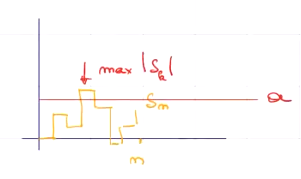
\includegraphics[width=0.6\linewidth]{screenshot017}
	\caption{The maximum of the random walk.}
	\label{fig:screenshot017}
\end{figure}
About this, we know that $\{S_{n}\}$ is a $\F$-martingale but in proving the Kolmogorov's inequaility we never talked about the martingale property! We could improve this inequality using the \emph{Doob's martingale inequality}. The problem is that we can prove very general inequalities that hold true for any \rv s but specifying more characteristic we can obtain stricter bounds. In this framework let's define 
\begin{equation*}
	\begin{array}{l}
		M^{\star}_{n}=\max_{k\leq n}M_{k}\\
		m^{\star}_{n}=\min_{k\leq n}M_{k}\\
	\end{array}
\end{equation*}
as current maximum and current minimum of $M$.
\begin{theorem}
	Take $M$ as a sub-martingale. For $b>0$ it holds:
	\begin{enumerate}
		\item $b\pr(M^{\star}_{n}\geq b)\leq\ev\left[M_{n}\indi_{\{M_{n}^{\star}\geq b\}}\right]\leq\ev\left[M_{n}^{+}\right]$;
		\item $b\pr(m^{\star}_{n}\leq-b)\leq-\ev M_{0}+\ev\left[M_{n}\indi_{\{m_{n}^{\star}\geq b\}}\right]\leq\ev M_{n}^{+}-\ev M_{0}$.
	\end{enumerate}
\end{theorem}
So we can further bound the result looking into the property of $M_{n}$.
\begin{example}
	Now need to define the brownian motion (or Weiner process).
	\begin{definition}
		A real-valued stochastic process $B={(B_{t})}_{t\geq0}$ is called \emph{brownian motion} if:
		\begin{enumerate}
			\item the index set is $\R^{+}$;
			\item $B_{0}(\omega)=0$ for almost all $\omega$;
			\item $B_{t_{n}}-B_{t_{n-1}},\ldots,B_{t_{1}}-B_{t_{0}}$ are independent for $\every 0=t_{0}<t_1<\ldots<t_n<\infty$;
			\item $B_{t}-B_{s}\sim B_{t+b}-B_{s+b}$ for every $0\leq s<t<\infty\quad\every n>- s$;
			\item $B_{t}-B_{s}\sim N(0,t-s)$;
			\item $t\mapsto B_{t}(\omega)$ are continuous for every $\omega$.
		\end{enumerate}
	\end{definition}
	The brownian motion is in itself a martingale, but there is a class of martingales strictly related to it:
	\begin{equation*}
		M_{t}=\exp\left\{\lambda B_{t}-\frac{1}{2}\lambda^{2}t\right\},\qquad t\in\R^{+}.
	\end{equation*}
	Now we can get to the actual example: if $B$ is a brownian motion, we have 
	\begin{equation*}
		\pr(\sup_{0\leq t\leq\theta}B_{t}\geq b)\leq\exp\left\{-\frac{b^{2}}{s\theta}\right\}.
	\end{equation*}
	The sample paths of brownian motions are extremely irregular. We are asking with which probability the max of our process will be over $b$ at time $\theta$.
	\begin{figure}[H]
		\centering
		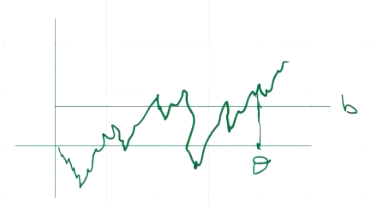
\includegraphics[width=0.6\linewidth]{screenshot018}
		\label{fig:screenshot018}
	\end{figure}
	I am basically asking if the maximum attained is above or below $b$.
	How can we use the Doob's inequality?
	\begin{fancyproof}
		Consider
		\begin{equation*}
			\pr(\sup B_{t}\geq b)=\pr(\sup e^{\lambda B_{t}}\geq e^{\lambda b})
		\end{equation*}
		and using Doob's inequality
		\begin{align*}
			\pr(\sup B_{t}\geq b)&=\pr(\sup e^{\lambda B_{t}}\geq e^{\lambda b})\\
			&\leq \frac{\overbrace{\ev\left[e^{\lambda B_{\theta}-\frac{\lambda^{2}}{2}\theta}\right]}^{\text{martingale}}}{e^{\lambda b}e^{-\frac{\lambda^{2}}{2}\theta}}\\
			&=e^{-\lambda b+\frac{\lambda^{2}}{2}\theta}\qquad\every\lambda>0
		\end{align*}
	\end{fancyproof}
\end{example}
\subsection{Predictable processes and Doob’s decomposition}
\begin{definition}
	The process $F={(F_{n})}_{n\geq1}$ is \emph{$\F$-predictable} if $F_{0}\in\F_{0}$ and $\F_{n+1}\in\F_{n}$, for $\every n\in\N$.
\end{definition}
This means that the available information up to $n$ is ``enough'' to have a bet in the period $n+1$. Some predictable processes are:
\begin{itemize}
	\item any deterministic processes;
	\item consider two stopping times $S,T$ of $\F$ and let $S\leq T$. Consider the \rv{} $V$ in $\F_{n}$. Then
	\[\begin{array}{c c c c}
		\color{DodgerBlue3}(1)&\color{DodgerBlue3}(2)&\color{DodgerBlue3}(3)&\color{DodgerBlue3}(4)\\
		V\indi_{(S,T]}&V\indi_{(S,\infty]}&\indi_{(S,T]}&\indi_{(0,T]}
	\end{array}\]
	are predictable processes.
	\begin{fancyproof}
		\begin{enumerate}
			\item[\color{DodgerBlue3}(2)] Consider $F=V\indi_{(S,\infty]}$, so that $F_{n}=\indi_{(S,\infty]}(n)$. Consider \begin{align*}
				F_{n+1}&=V\indi_{(S,\infty]}(n+1)\\
				&=V\indi_{\{S<n+1\}}\\
				&=V\indi_{\{S\leq n\}}\in\F_{n}
			\end{align*}
			so the process is $\F$-measurable and predictable.
			\item[\color{DodgerBlue4}(1)] Since we know by hypothesis that $S\leq T$ then $V\in\F_{S}\subset\F_{T}$. This means that $V\in\F_{T}$. Hence, of a consequence,
			\begin{equation*}
				V\indi_{(T,\infty]}-V\indi_{(S,\infty]}=V\indi_{(S,T]}
			\end{equation*}
			is predictable.
			\item[\color{DodgerBlue3}(3)] Take $V=1$.
			\item[\color{DodgerBlue3}(4)] Take $T=\infty$, $V=1$. $\indi_{(S,\infty]}$ is predictable. But then 
			\[\indi_{[0,S]}=\indi-\indi_{(S,\infty]}\]
			so it is predictable.
		\end{enumerate}
	\end{fancyproof}
\end{itemize}
\begin{theorem}
	\emph{Doob's decomposition}.\\
	$X$ is a stochastic process which is adapted to $\F$ and integrable. Then
	\begin{enumerate}
		\item it can be decomposed as 
		\[X_{n}=X_{0}+M_{n}+A_{n},\qquad n\in\N\]
		where:
		\begin{itemize}
			\item $M_{n}$ is a $\F$-martingale with $M_0=0$;
			\item $A_{n}$ is a predictable process with $A_0=0$.
		\end{itemize}
		\item The decomposition is unique up to equivalence.
		\item If $X_{n}$ is a sub-martingale then ${\{A_{n}\}}_{n\geq0}$ increasing, while if $X_{n}$ is a super-martingale then ${\{A_{n}\}}_{n\geq0}$ is decreasing.
	\end{enumerate}
\end{theorem}
\begin{fancyproof}
	Put $A_0=M_0=0$. Define $M$ and $A$ through their increments:
	\[ \begin{array}{l l}
		A_{n+1}-A_{n}&=\underbracket[0.3pt]{\ev\Big[X_{n+1}-X_{n}|\F_{n}\Big]}_{\F_{n}-\text{meas.}}\\
		M_{n+1}-M_{n}&=(X_{n+1}-X_{n})-(A_{n+1}-A_{n}).
	\end{array} \]
	If we look at these quantities we see that $A$ is predictable and $M$ is martingale. Imagine now there is another decomposition: let
	\[X=X_0+M'+A'\]
	be another decomposition. We must have
	\[\cancel{X_0}+M'+A'=\cancel{X_0}+M+A\iff A-A'=M-M'=B.\]
	Now $B$ is a process and it is predictable and martingale (because it is the difference between two martingales). Since $B$ is predictable \textit{and} a martingale we have
	\begin{align*}
		B_{n+1}-B_{n}&\underset{\mathclap{\text{\tiny predictable}}}{=}\ev[B_{n+1}-B_{n}|\F_{n}]\\
		&\underset{\mathclap{\text{\tiny martingale}}}{=}0\\
		&\implies B_{n+1}=B_{n}=B_0\;\as,A=A'\;\as,M=M'\as\\
	\end{align*}
	If $X$ is a sub-martingale then we have
	\[\ev[X_{n+1}-X_{n|\F_{n}}]\geq0\]
	and this means that we have $A_{n+1}\geq A_{n}$ is increasing.
\end{fancyproof}
\subsection{Doob’s stopping theorem}
For a martingale we know
\[\ev[X_{t}-X_{s}|\F_{s}]=0.\]
The question is: is this true also if $s$ and $t$ are substituted by stopping times $S,T,S\leq T$?
\begin{theorem}
	Let $M$ be adapted to $\F$. Then the following are equivalent:
	\begin{enumerate}[\circnum]
		\item $M$ is a submartingale;
		\item for every bounded stopping time $S\leq T$ the \rv s $M_{S}$ and $M_{T}$ are integrable and 
		\[\ev[M_{T}-M_{S}|\F_{S}]\geq0;\]
		\item for each pair of bounded stopping times the \rv s $M_{S}$ and $M_{T}$ are integrable and 
		\[\ev[M_{T}-M_{S}]\geq 0.\] 
	\end{enumerate}
\end{theorem}
\begin{remark}
	If $M$ is a martingale the theorem can be read in a different way:
	\begin{equation*}
		\ev M_{T}=\ev M_{S}=\ev M_{0}.
	\end{equation*}
	Previously, $\ev M_{n}=\ev M_{n-1}=\ev M_{0}$.
\end{remark}
\begin{fancyproof}
	To prove the theorem we need to show that from condition 1 follows 2 from which follows 3 from which follows 1.
	\begin{enumerate}
		\item[$1\to 2$] by hypothesis $M$ is a sub-martingale and our thesis is that if $S(\omega)<T(\omega)<n$ (because we asked for bounded times) then:
		\begin{enumerate}
			\item $M_{S}$ and $M_{T}$ are integrable;
			\item $\ev[M_{T}-M_{S}|\F_{S}]\geq0$.
		\end{enumerate}
		We know that $S$ and $T$ are bounded by $n$. Let $V$ be a positive bounded \rv{} and define $F=V\indi_{(S,T]}$ and use it in the discrete time integral:
		\[X_{n}=\underbrace{M_0F_0}_{X_0}+(M_1-M_0)\underbrace{F_1}_{\mathclap{V\indi_{\{1\in(S,T]\}}}}+\ldots+(M_{n}-M_{n-1})F_{n}\]
		So we have 
		\[X_{n}-X_{0}=V(M_{T}-M_{S})\]
		So $X_{n}$ is a sub-martingale. Take $V=1$ and $S=0$: now we have
		\begin{equation*}
			\begin{array}{c c c l}
				X_{n}&-&X_{0}&=M_{T}\\
				\downarrow&&\downarrow&\\
				\text{int.}&&\text{int.}&\implies M_{T}\text{ is integrable}.
			\end{array}
		\end{equation*}
		Now take $V=1$ and $T=n$ so that we get
		\begin{equation*}
			\begin{array}{c c c c l}
				X_{n}&-&X_{0}&=M_{n}&-M_{S}\\
				\downarrow&&\downarrow&\downarrow&\\
				\text{int.}&&\text{int.}&\text{int.}&\implies M_{S}\text{ is integrable}.
			\end{array}
		\end{equation*}
		We recall that $V\in\F_S$ and we use the defining property for $\ev(\cdot|\F_S)$. So we can write
		\begin{align*}
			\ev V\ev(M_{T}-M_{S}|\F_{S})&\underset{\mathclap{\text{def. prop.}}}{=}\ev V(M_{T}-M_{S})\\
			&\underset{\mathllap{\text{discr. time int.}}}{=}\ev[X_{n}-X_{0}]\\
			&\underset{\mathllap{\text{proved above}}}{\geq}0
		\end{align*}
		and this is true $\every V>0,V<b,V\in\F_{s}$. Hence
		\begin{equation*}
			\ev(M_{T}-M_{S}|\F_{S})\geq 0
		\end{equation*}
		So $1\to2$.
		\item[$2\to3$] We can use the tower rule. Take the expectation of point 2:
		\[\ev[\ev(M_{T}-M_{S}|\F_{S})]=\ev[M_{T}-M_{S}]\geq0.\]
		\item[$3\to1$] Let $3$ hold, so that $\ev[M_{T}-M_{S}]\geq0$. Choose $T=n$ and $S=0$. Then
		$M_{n}$ is integrable. Move to adaptness: this holds by hypothesis. Move to the martingale inequality:
		\begin{equation*}
			\ev[M_{n}-M_{m}|\F_{m}]\geq0.
		\end{equation*}
		Note that this is equivalent to prove 
		\begin{equation*}
			\ev\indi_H\ev[M_{n}-M_{m}|\F_{m}]\geq0\qquad H\in\F_{m},0\leq m\leq n.
		\end{equation*}
		Fix $H,m,n$ and define
		\begin{equation*}
			S(\omega)=m\qquad T(\omega)=n\indi_H(\omega)+m\indi_{\{\Omega\setminus H\}}(\omega)
		\end{equation*}
		The indicators are non-zero in complementary instances. Notice that:
		\begin{enumerate}
			\item $S$ is a fixed time so it is a stopping time;
			\item $S\leq T\leq n$ by definition of $S$ and $T$ because the indicators are non-zero in complementary instances;
			\item $T\geq S$ is a foretold time by $S=m$;
			\item $H\in\F_{S}$ by definition.
		\end{enumerate}
		So we can write $M_{T}-M_{S}=\indi_H(M_{n}-M_{m})$ where $M_{T}-M_{S}\geq0$ by hypothesis. This means that we have 
		\begin{equation*}
			\underbrace{\ev[\indi_{H}\ev(M_{n}-M_{m}|\F_{m})]}_{\ev[M_{n}-M_{m}|\F_{m}]\geq0}\geq0
		\end{equation*}
	\end{enumerate}
\end{fancyproof}
\subsection{Upcrossing inequality} 
I believe that what is being asked is
\begin{proposition}
	If $M$ is a sub-martingale with respect to its natural filtration then 
	\begin{equation*}
		(b-a)\ev U_{n}(a,b)\leq\ev\left[(M_{n}-a)^{+}-(M_{0}-a)^{+}\right].
	\end{equation*}
\end{proposition}
We wanted to find a bound for our profit, but our profit is a stochastic quantity: so it's only natural to think about the expectation to give a bound to the number of expected up/downcrossing.\\
Observe that the number of upcrossings does not depend on the value of $T_0$ that we fix.
\begin{fancyproof}
	Choose $a=0$. Consider hence the process $(M-a)^{+}$ that is sub-martingale (if $M$ is a sub-martingale). Take $M\geq 0$ and let 
	\begin{equation*}
		F_{n}-\sum_{k=1}^{\infty}\indi_{(S_{k},T_{k}]}(n)
	\end{equation*}
	and consider 
	\begin{equation*}
		X=\int F\dif M
	\end{equation*}
	like in our example. We know that $F$ is predictable since by definition $F_{k+1}\in\F_{k}$. Consider the expectation of the increment
	\begin{equation*}
		\ev[X_{k+1}-X_{k}|\F_{k}]=\ev\left[F_{k+1}(M_{k+1}-M_{k})|\F_{k}\right].
	\end{equation*}
	But since $F_{k+1}$ is predictable we can take it out the expectation:
	\begin{equation*}
		F_{k+1}\ev\left[M_{k+1}-M_{k}|\F_{k}\right].
	\end{equation*}
	But since $F_{k+1}$ is an indicator we know it is $\leq1$:
	\begin{equation*}
		\ev[X_{k+1}-X_{k}|\F_{k}]\leq\ev\left[M_{k+1}-M_{k}|\F_{k}\right].
	\end{equation*}
	Now take the expectation of both sides:
	\begin{equation*}
		\ev[X_{k+1}-X_{k}]\leq\ev\left[M_{k+1}-M_{k}\right].
	\end{equation*}
	If we sum these inequalities over $k$ we get:
	\begin{equation*}
		\ev\left[X_{n}-X_{0}\right]\leq\ev\left[M_{n}-M_{0}\right].
	\end{equation*}
	So we now get that
	\begin{equation*}
		bU_{n}(a,n)\leq\ev\left[X_{n}-X_{0}\right]\leq\ev\left[M_{n}-M_{0}\right]
	\end{equation*}
	but given that $a=0$ we get that
	\begin{equation*}
		bU_{n}(0,b)\leq\ev[M_{n}-M_{0}].
	\end{equation*}
	Clearly we have to take the positive part.
\end{fancyproof}
But I also found this
\begin{proposition}
Suppose that $\{X={X_{t}:t\in[0,\infty)}\}$ satisfies the basic assumptions with respect to the filtration $\F=\{\F_t:t\in[0,\infty)\}$ and let $a,b\in\R$ with $a<b$. Let $U_{t}=u_{t}(a,b,X)$ the random number of upcrossings of $[a,b]$ by $X$ up to time $t\in[0,\infty)$. 
\begin{enumerate}[\circnum]
	\item if $X$ is a super-martingale relative to $\F$ then
	\begin{equation*}
		\ev(U_{t})\leq\frac{1}{b-a}\ev\left[(X_{t}-a)^{-}\right]\leq\frac{1}{b-a}\left[\ev(X_{t}^-)+|a|\right]\leq\frac{1}{b-a}\left[\ev(|X_{t}|)+|a|\right];
	\end{equation*}
	\item if $X$ is a sub-martingale relative to $\F$ then
	\begin{equation*}
			\ev(U_{t})\leq\frac{1}{b-a}\ev\left[(X_{t}-a)^{+}\right]\leq\frac{1}{b-a}\left[\ev(X_{t}^+)+|a|\right]\leq\frac{1}{b-a}\left[\ev(|X_{t}|)+|a|\right];
	\end{equation*}
\end{enumerate}	
\end{proposition}
\subsection{Doob’s decomposition}
\begin{theorem}
\emph{Doob's decomposition}.\\
$X$ is a stochastic process which is adapted to $\F$ and integrable. Then
\begin{enumerate}
	\item it can be decomposed as 
	\[X_{n}=X_{0}+M_{n}+A_{n},\qquad n\in\N\]
	where:
	\begin{itemize}
		\item $M_{n}$ is a $\F$-martingale with $M_0=0$;
		\item $A_{n}$ is a predictable process with $A_0=0$.
	\end{itemize}
	\item The decomposition is unique up to equivalence.
	\item If $X_{n}$ is a sub-martingale then ${\{A_{n}\}}_{n\geq0}$ increasing, while if $X_{n}$ is a super-martingale then ${\{A_{n}\}}_{n\geq0}$ is decreasing.
\end{enumerate}
\end{theorem}
\begin{fancyproof}
Put $A_0=M_0=0$. Define $M$ and $A$ through their increments:
\[ \begin{array}{l l}
	A_{n+1}-A_{n}&=\underbracket[0.3pt]{\ev\Big[X_{n+1}-X_{n}|\F_{n}\Big]}_{\F_{n}-\text{meas.}}\\
	M_{n+1}-M_{n}&=(X_{n+1}-X_{n})-(A_{n+1}-A_{n}).
\end{array} \]
If we look at these quantities we see that $A$ is predictable and $M$ is martingale. Imagine now there is another decomposition: let
\[X=X_0+M'+A'\]
be another decomposition. We must have
\[\cancel{X_0}+M'+A'=\cancel{X_0}+M+A\iff A-A'=M-M'=B.\]
Now $B$ is a process and it is predictable and martingale (because it is the difference between two martingales). Since $B$ is predictable \textit{and} a martingale we have
\begin{align*}
	B_{n+1}-B_{n}&\underset{\mathclap{\text{\tiny predictable}}}{=}\ev[B_{n+1}-B_{n}|\F_{n}]\\
	&\underset{\mathclap{\text{\tiny martingale}}}{=}0\\
	&\implies B_{n+1}=B_{n}=B_0\;\as,A=A'\;\as,M=M'\as\\
\end{align*}
If $X$ is a sub-martingale then we have
\[\ev[X_{n+1}-X_{n|\F_{n}}]\geq0\]
and this means that we have $A_{n+1}\geq A_{n}$ is increasing.
\end{fancyproof}
\subsection{Stochastic integral in discrete time}
Let us consider two real-valued processes $M={(M_{n})}_{n}$ and $F={(F_{n})}_{n}$ and let us define
\[X_{n}=F_0M_{0}+(M_1-M_0)F_1+\ldots+(M_{n}-M_{n-1})F_n.\]
We say that $\{X_{n}\}$ is the integral of $F$ with respect to $M$ and we write
\[X_{n}=\int F \dif M\]
where $\dif M$ is a random signed measure. Remember the Lebesgue-Stieltjes integral? Me neither, but as long as $M$ has bounded variation this is a Lebesgue-Stieltjes integral. So a little explanation is due since I actually never saw a Stieltjes integral.
\begin{theorem}
	Consider $F$ bounded and predictable. Then if $M$ is a martingale then $X$ is a martingale; If $M$ is a sub(super)-martingale then $X$ is a sub(super)-martingale.
\end{theorem}
This means that... \emph{we can't beat the system!}
\begin{flushright}
	\begin{tikzpicture}
		\calloutquote[width=4cm,position={(1,-1)},fill=Turquoise4!30,rounded corners]{I can beat something else though.}
	\end{tikzpicture}\hspace*{2.5cm}
\end{flushright}
\begin{example}
	Consider $M_{n}$ as the price of a share at time $n$ and $F_{n}$ as the number of shares owned during $(n-1,n]$. Our profit will be 
	\[(M_{n}-M_{n=1})F_{n}\]
	and our total profit $X_{n}$ gained during $(0,n]$ will be:
	\[X_{n}=X_{0}+\underbrace{\sum_{k=1}^{n}(M_{k}-M_{k-1})F_{k}}_{\mathclap{\text{discrete time integral}}}\]
	$F_{n}$ is based on the knowledge in $n-1$ so it is predictable. The process $M_{n}$ should be a martingale (otherwise if it is a sub/super-martingale everyone/no one will buy). So the total profit will also be a martingale! We can only choose our buying politics $F_{k}$, but there is no way to select a politics that will change a martingale in a super-martingale or sub-martingale.
\end{example}
Clearly this works in mean! 
\begin{fancyproof}
	\begin{enumerate}
		\item	We have $M$ being a martingale and $F_0,F_1,\ldots,F_n\in\F_{n}$ as well as $M_0,M_1,\ldots,M_{n}\in\F_n$. Therefore $X_{n}\in\F_{n}$ and $X$ is adapted to $\F$.
		\item We need to check whether the discrete time integral is a martingale. We know by hypothesis that $F$ is bounded, so $F<b$ for some $b$. This implies
		\begin{equation*}
			|X_{n}|<b(|M_{0}|+|M_1+M_0|+\ldots+|M_n-M_{n-1}|)
		\end{equation*}
		Since $M$ is a martingale and it is integrable, we get that $X_n$ is bounded and integrable.
		\item Consider
		\begin{equation*}
			\ev[X_{n+1}-X_{n}|\F]=\ev[F_{n+1}(M_{n+1}-M_{n})|\F_n]
		\end{equation*}
		since all the terms cancel out and only the last ones survive. But $F_{n+1}\in\F_{n}$ so we can take it out of the expectation:
		\[F_{n}\underbrace{\ev[M_{n+1}-M_{n}|\F_{n}]}_{=0}=0.\]
	\end{enumerate}
\end{fancyproof}
\subsection{Stochastic integral and its application}
Let us consider two real-valued processes $M={(M_{n})}_{n}$ and $F={(F_{n})}_{n}$ and let us define
\[X_{n}=F_0M_{0}+(M_1-M_0)F_1+\ldots+(M_{n}-M_{n-1})F_n.\]
We say that $\{X_{n}\}$ is the integral of $F$ with respect to $M$ and we write
\[X_{n}=\int F \dif M\]
where $\dif M$ is a random signed measure. Remember the Lebesgue-Stieltjes integral? Me neither, but as long as $M$ has bounded variation this is a Lebesgue-Stieltjes integral. So a little explanation is due since I actually never saw a Stieltjes integral.
\begin{theorem}
	Consider $F$ bounded and predictable. Then if $M$ is a martingale then $X$ is a martingale; If $M$ is a sub(super)-martingale then $X$ is a sub(super)-martingale.
\end{theorem}
This means that... \emph{we can't beat the system!}
\begin{flushright}
	\begin{tikzpicture}
		\calloutquote[width=4cm,position={(1,-1)},fill=Turquoise4!30,rounded corners]{I can beat something else though.}
	\end{tikzpicture}\hspace*{2.5cm}
\end{flushright}
\begin{example}
	Consider $M_{n}$ as the price of a share at time $n$ and $F_{n}$ as the number of shares owned during $(n-1,n]$. Our profit will be 
	\[(M_{n}-M_{n=1})F_{n}\]
	and our total profit $X_{n}$ gained during $(0,n]$ will be:
	\[X_{n}=X_{0}+\underbrace{\sum_{k=1}^{n}(M_{k}-M_{k-1})F_{k}}_{\mathclap{\text{discrete time integral}}}\]
	$F_{n}$ is based on the knowledge in $n-1$ so it is predictable. The process $M_{n}$ should be a martingale (otherwise if it is a sub/super-martingale everyone/no one will buy). So the total profit will also be a martingale! We can only choose our buying politics $F_{k}$, but there is no way to select a politics that will change a martingale in a super-martingale or sub-martingale.
\end{example}
Clearly this works in mean! 
\begin{fancyproof}
	\begin{enumerate}
		\item	We have $M$ being a martingale and $F_0,F_1,\ldots,F_n\in\F_{n}$ as well as $M_0,M_1,\ldots,M_{n}\in\F_n$. Therefore $X_{n}\in\F_{n}$ and $X$ is adapted to $\F$.
		\item We need to check whether the discrete time integral is a martingale. We know by hypothesis that $F$ is bounded, so $F<b$ for some $b$. This implies
		\begin{equation*}
			|X_{n}|<b(|M_{0}|+|M_1+M_0|+\ldots+|M_n-M_{n-1}|)
		\end{equation*}
		Since $M$ is a martingale and it is integrable, we get that $X_n$ is bounded and integrable.
		\item Consider
		\begin{equation*}
			\ev[X_{n+1}-X_{n}|\F]=\ev[F_{n+1}(M_{n+1}-M_{n})|\F_n]
		\end{equation*}
		since all the terms cancel out and only the last ones survive. But $F_{n+1}\in\F_{n}$ so we can take it out of the expectation:
		\[F_{n}\underbrace{\ev[M_{n+1}-M_{n}|\F_{n}]}_{=0}=0.\]
	\end{enumerate}
\end{fancyproof}
and for the applications:\\
\begin{definition}
	Define $M={(M_{n})}_{n\in\N}$ as a process and let $T$ be a random time with values on $\overline{\N}$. The process
	\[X_{n}(\omega)=M_{n\wedge T}(\omega)=\begin{cases}
		M_{n}(\omega)&n<T(\omega)\\
		M_{T}(\omega)&n>T(\omega)
	\end{cases}\]
	(where $n\wedge T$ is a truncated random time) is called \emph{$M$ stopped at $T$}.
\end{definition}
As a consequence $X$ is exactly the discrete time integral if $F=\indi_{[0,T]}$:
\begin{equation*}
	X_{n}=\underbracket[0.6pt]{M_0F_0}_{0}+(M_{1}+M_{0})\indi_{[0,T]}(1)+\ldots+(M_{n}-M_{n-1})\indi_{[0,T]}(n).
\end{equation*}
The indicators only select the current time interval. If this is the case we can observe that $F_{[0,T]}$ is bounded, positive and predictable. Hence if $M$ is a martingale the theorem applies with this special choice of $M$ and we can write the result as a different theorem:
\begin{theorem}
	Let $T$ be a stopping time and let $X$ be the process $M$ stopped at $T$. If $M$ is a martingale then so is $X$ (the same holds for sub-martingales and super-martingales).
\end{theorem}
So we cannot determine a policy based on stopping times that can change the nature of our martingale. In the remote case in which you are interested in this you can read Williams - Introduction to martingales. \\
\subsection{Impossibility to win against the system: related theorems and examples}
\begin{theorem}
	Consider $F$ bounded and predictable. Then if $M$ is a martingale then $X$ is a martingale; If $M$ is a sub(super)-martingale then $X$ is a sub(super)-martingale.
\end{theorem}
This means that... \emph{we can't beat the system!}
\begin{flushright}
	\begin{tikzpicture}
		\calloutquote[width=4cm,position={(1,-1)},fill=Turquoise4!30,rounded corners]{I can beat something else though.}
	\end{tikzpicture}\hspace*{2.5cm}
\end{flushright}
\begin{example}
	Consider $M_{n}$ as the price of a share at time $n$ and $F_{n}$ as the number of shares owned during $(n-1,n]$. Our profit will be 
	\[(M_{n}-M_{n=1})F_{n}\]
	and our total profit $X_{n}$ gained during $(0,n]$ will be:
	\[X_{n}=X_{0}+\underbrace{\sum_{k=1}^{n}(M_{k}-M_{k-1})F_{k}}_{\mathclap{\text{discrete time integral}}}\]
	$F_{n}$ is based on the knowledge in $n-1$ so it is predictable. The process $M_{n}$ should be a martingale (otherwise if it is a sub/super-martingale everyone/no one will buy). So the total profit will also be a martingale! We can only choose our buying politics $F_{k}$, but there is no way to select a politics that will change a martingale in a super-martingale or sub-martingale.
\end{example}
Clearly this works in mean! 
\begin{fancyproof}
	\begin{enumerate}
		\item	We have $M$ being a martingale and $F_0,F_1,\ldots,F_n\in\F_{n}$ as well as $M_0,M_1,\ldots,M_{n}\in\F_n$. Therefore $X_{n}\in\F_{n}$ and $X$ is adapted to $\F$.
		\item We need to check whether the discrete time integral is a martingale. We know by hypothesis that $F$ is bounded, so $F<b$ for some $b$. This implies
		\begin{equation*}
			|X_{n}|<b(|M_{0}|+|M_1+M_0|+\ldots+|M_n-M_{n-1}|)
		\end{equation*}
		Since $M$ is a martingale and it is integrable, we get that $X_n$ is bounded and integrable.
		\item Consider
		\begin{equation*}
			\ev[X_{n+1}-X_{n}|\F]=\ev[F_{n+1}(M_{n+1}-M_{n})|\F_n]
		\end{equation*}
		since all the terms cancel out and only the last ones survive. But $F_{n+1}\in\F_{n}$ so we can take it out of the expectation:
		\[F_{n}\underbrace{\ev[M_{n+1}-M_{n}|\F_{n}]}_{=0}=0.\]
	\end{enumerate}
\end{fancyproof}
We know that using a policy that it is predictable it is impossible to beat the system. Finance bros try to overcome this possibility using stopping times. If my policy is not only based on a predictable process but I add the randomness of the time in which I decide to sell or buy can I break the curse of martingales and make shareholders want to suck my dick? Well, it depends.
\subsection{Predictable and adapted processes: definition and examples}
\begin{definition}
	The process $F={(F_{n})}_{n\geq1}$ is \emph{$\F$-predictable} if $F_{0}\in\F_{0}$ and $\F_{n+1}\in\F_{n}$, for $\every n\in\N$.
\end{definition}
This means that the available information up to $n$ is ``enough'' to have a bet in the period $n+1$. Some predictable processes are:
\begin{itemize}
	\item any deterministic processes;
	\item consider two stopping times $S,T$ of $\F$ and let $S\leq T$. Consider the \rv{} $V$ in $\F_{n}$. Then
	\[\begin{array}{c c c c}
		\color{DodgerBlue3}(1)&\color{DodgerBlue3}(2)&\color{DodgerBlue3}(3)&\color{DodgerBlue3}(4)\\
		V\indi_{(S,T]}&V\indi_{(S,\infty]}&\indi_{(S,T]}&\indi_{(0,T]}
	\end{array}\]
	are predictable processes.
	\begin{fancyproof}
		\begin{enumerate}
			\item[\color{DodgerBlue3}(2)] Consider $F=V\indi_{(S,\infty]}$, so that $F_{n}=\indi_{(S,\infty]}(n)$. Consider \begin{align*}
				F_{n+1}&=V\indi_{(S,\infty]}(n+1)\\
				&=V\indi_{\{S<n+1\}}\\
				&=V\indi_{\{S\leq n\}}\in\F_{n}
			\end{align*}
			so the process is $\F$-measurable and predictable.
			\item[\color{DodgerBlue4}(1)] Since we know by hypothesis that $S\leq T$ then $V\in\F_{S}\subset\F_{T}$. This means that $V\in\F_{T}$. Hence, of a consequence,
			\begin{equation*}
				V\indi_{(T,\infty]}-V\indi_{(S,\infty]}=V\indi_{(S,T]}
			\end{equation*}
			is predictable.
			\item[\color{DodgerBlue3}(3)] Take $V=1$.
			\item[\color{DodgerBlue3}(4)] Take $T=\infty$, $V=1$. $\indi_{(S,\infty]}$ is predictable. But then 
			\[\indi_{[0,S]}=\indi-\indi_{(S,\infty]}\]
			so it is predictable.
		\end{enumerate}
	\end{fancyproof}
\end{itemize} 
Example of adapted process:
\begin{example}
	This is called ``the secretary problem'': in this case we must start from the filtration and then understand the problem.
	Here i have $N$ candidates for a position; a candidate disregarded after the interview is lost. The interviewer wants to hire exactly 1 candidate and each candidate has different abilities and the interviewer knows only the relative ability of those already interviewed so far. Our goal is to maximizing the probability of hiring the best one. We have three questions:
	\begin{enumerate}
		\item what is $\Omega$?
		\item what is the filtration $\F$ for this experiment?
		\item what process should we use?
	\end{enumerate}
	In this case $\Omega=N!$ permutations of the ranking of the candidates (the order in which they show up) and the filtration is the information earned from interview up to time $t$ (that is the ranking of the candidates up to time $t$). But what is the process that I should use? Consider the sequence
	\[V_1,V_2,\ldots\qquad{\{V_i\}}_{i\geq 1}\]
	with $V_i=1$ if and only if the best candidate is the $i$-th candidate and $V_i=0$ otherwise. Could this process ${\{V_i\}}_{i\geq 1}$ be used? No, because $V$ is not adapted to $\F$... because to understand if $i$-th candidate is te best we need to compare it to the other candidates, including the ones that didn't show up yet! But then how can we get an adapted process? Let us consider the expectation
	\[U_n=\ev\left[V_n|\F_n\right]\]
	What do we know about the measurability of $U_n$? We know that it is for sure $\F_n$-measurable. This trick gives us a simple way to build an adapted process. So now we will have:
	$U_n=
	0$ if the candidate is not the best up to $n$ and $U_n=1$ otherwise. More specifically, we will have
	\begin{align*}
		U_n&=1\cdot\substack{\text{proability that the best candidate}\\\text{is among the first $n$}}+0\cdot\substack{\text{proability that the best candidate}\\\text{is not among the first $n$}}\\
		&=1\cdot\frac{n}{N}+0\cdot\frac{N-n}{N}.\\
		&=\frac{n}{N}
	\end{align*}
	This is a quantity that I can measure and it is therefore adapted.\par
\end{example}
\subsection{Poisson process and its martingale property}
Consider $\R_+$ as our index set. $\F$ is our filtration and we consider the counting process $N={(N_{t})}_{y\geq0}$: this counts the number of events up to time $t$, it has unit jumps and any path starts from 0 so that $N_{0}(\omega)=0$, it is increasing and it is right continuous.
\begin{definition}
	The counting process $N$ is said to be a \emph{Poisson process} with rate $\lambda$ with respect to $\F$ if it is adapted to $\F$ and
	\[\ev[f(N_{t+s}-N_s)|\F_s]=\sum_{k=0}^{\infty}e^{-\lambda t}\frac{(\lambda t)^{k}}{k!}f(k)\qquad\every s,t\in\R_+,\every\text{positive }f\mapsto\N.\]
\end{definition}
\begin{theorem}
	Let $N$ be a counting process. It is a Poisson process with rate $\lambda$ with respect to $\F$ \ifonly{}:
	\begin{equation*}
		M_{t}=N_{t}-\lambda t
	\end{equation*}
	is a $\F$-martingale.
\end{theorem}
We only prove that $M_t$ is a martingale if $N_{t}$ is Poisson.
\begin{fancyproof}
	We know that 
	\begin{align*}
		\ev[M_{t}|\F_{s}]&=\ev[M_{t}-M_{s}+M_{s}|\F_{s}]\\
		&=\ev[M_{t}-M_{s}|\F_{s}]+M_{s}\\
		&=\ev[M_{t}-M_{s}]+M_{s}\\
		&=\ev[N_{t}-N_{s}+\lambda t+\lambda s]+M_{s}\\
		&=\underbrace{\ev[N_{t}-N_{s}]}_{\cancel{\lambda (t-s)}}-\cancel{\lambda (t-s)}+M_{s}\\
		&=M_{s}
	\end{align*}
\end{fancyproof}
\subsection{Stopped processes and their properties}
\begin{example}
	Some stopping times:
	\begin{enumerate}[\circnum]
		\item The first time that $X(\omega)\in H\in\Omega$;
		\[T(\omega)=\begin{cases}
			\inf \left\{n\in\N:X_n(\omega)\in H\right\}&\\
			+\infty&\text{if $X_n(\omega)\notin H\;\every n$}
		\end{cases}\]
		So
		\[\left\{T\leq n\right\}=\bigcup_{k=0}^{n}\left\{X_k\in H\right\}.\]
		\item Consider i.i.d. \rv{}s 
		$X_1,X_2,\ldots$. Consider the probabilities
		\[\pr(X_i=1)=\pr(X_i=-1)=\frac{1}{2}\]
		and the random walk
		\[S_n=\sum_{1}^{n}X_i.\]
		Let's define 
		\[T_1=\begin{cases}
			\min\left\{n<50:S_n=3\right\}\\
			50 &\text{otherwise}.
		\end{cases}\]
		This is a stopping time because I can write $\left\{T_1\leq n\right\}$ as $$\underbracket[0.6pt]{\bigcup_{k=1}^{n}\underbracket[0.6pt]{\left\{S_k=3\right\}}_{\text{$\F_k$-measurable}}}_{\mathclap{\text{$\F_n$-measurbale}}}\qquad n<50.$$
		Moreover for $n=50$ we have $T_{1}\in\F_{50}$.
		\item Starting from the previously deifned random walk, consider the quantity 
		\[M_n=\min(S_1,\ldots,S_n)\]
		And the random time
		\[T_2=\min\left\{n:S_n\geq M_m+2\right\}\]
		is a stoppimg time. On the contrary, 
		\[T_3=\begin{cases}
			\max\left\{n<50:S_n=7\right\}&\text{if not empty}\\
			50 &\text{otherwise}
		\end{cases}\]
		is not a stopping time. Why? Because I have to wait until $n=50$ to answer the question. 
	\end{enumerate}
\end{example}

Consider the random times on $\R_+$
\[0<T_1<T_2<\ldots\]
With $\lim_{n\to\infty}T_n=+\infty$. Define the process $\left\{N_t\right\}$ as 
\[N_t:=\sum\indi_{[0,t]}(T_n).\]
This is called \emph{counting process}. It is a basic count of the number of events happened up to time $n$.
$N_{t}$ is increasing, right continuous and incresases by unitary jumps. Moreover, $N_0=0$, $N_t<\infty$ for $t\in\R_+$. Of course $\lim_{t\to\infty}N_t=\infty$. Counting processes generate their natural filtration $\F$.

Some problems require to stop the observation at a stopping time (because we don't care anymore\footnote{Assuming we ever did.})... So we don't actually need the whole knowledge of the complete filtration $\F={\left(\F_t\right)}_{t\geq 0}$. The problem is that as we said before the stopping time is a random time. So what we need is the \textit{information known up to time $T$} $\F_T$, basically the $\sigma$-field that is the filtration at time $T$. 
\begin{example}
	\emph{Truncated stopping time}: let $T$ be a stopping time (for example, the time at which we sell certain shares) and that we want a finite horizon for this decision. In this case the quantity of interest is
	\begin{equation*}
		S=T\wedge n=\min\{T,n\}
	\end{equation*}
	where $n$ could be some sort of time horizon.\\
	Imagine that two cyclists participate to a race. Their children will have their snack when both the parents will arrive to the finish line. How long will the children wait for their snack?
	We can think about the following stopping times:
	\[ 	\begin{array}{l l}
		T: & \text{time employed by the first cyclist}\\
		S: & \text{time employed by the second cyclist}\\
		U: &\max\{S,T\}.
		
	\end{array} \]
	The waiting time for the children will be $U$.
\end{example}
\subsection{Important inequalities for sub-martingales}
The problem is that we can prove very general inequalities that hold true for any \rv s but specifying more characteristic we can obtain stricter bounds. In this framework let's define 
\begin{equation*}
	\begin{array}{l}
		M^{\star}_{n}=\max_{k\leq n}M_{k}\\
		m^{\star}_{n}=\min_{k\leq n}M_{k}\\
	\end{array}
\end{equation*}
as current maximum and current minimum of $M$.
\begin{theorem}
	Take $M$ as a sub-martingale. For $b>0$ it holds:
	\begin{enumerate}
		\item $b\pr(M^{\star}_{n}\geq b)\leq\ev\left[M_{n}\indi_{\{M_{n}^{\star}\geq b\}}\right]\leq\ev\left[M_{n}^{+}\right]$;
		\item $b\pr(m^{\star}_{n}\leq-b)\leq-\ev M_{0}+\ev\left[M_{n}\indi_{\{m_{n}^{\star}\geq b\}}\right]\leq\ev M_{n}^{+}-\ev M_{0}$.
	\end{enumerate}
\end{theorem}
So we can further bound the result looking into the property of $M_{n}$.
\begin{fancyproof}
	We introduce 2 stopping times: 
	\begin{equation*}
		\begin{array}{l l}
			T&=\inf\{n\geq0:M_{n}\geq b\}\\
			S&=\inf\{n\geq0:M_{n}\leq-b\}.
		\end{array}
	\end{equation*}
	\begin{figure}[H]
		\centering
		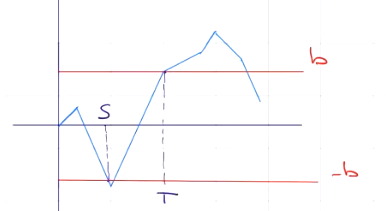
\includegraphics[width=0.6\linewidth]{screenshot019}
		\label{fig:screenshot019}
	\end{figure}
	Consider the current maximum and minimum above the level $b$:
	\begin{equation*}
		\{M^{\star}_{n}\geq b\}=\{T\leq n\}\qquad	\{m^{\star}_{n}<-b\}=\{S\leq n\}.
	\end{equation*}
	Fix $b$ and $n$. When $\{T\leq n\}$ we have
	\begin{align*}
		M_{T\wedge n}=M_{T}\geq b.
	\end{align*}
	Multiply by $\indi_{\{T\leq n\}}$:
	\begin{equation*}
		b\indi_{\{T\leq n\}}\leq M_{T\wedge m}\indi_{\{T\leq n\}}.
	\end{equation*}
	Using Doob's stopping theorem we know that 
	\begin{equation*}
		\ev\left[M_{T}-M_{S}|\F_{S}\right]\geq0
	\end{equation*}
	and using $S=T\wedge n$ and $T=n$ we obtain
	\begin{equation*}
		\ev\left[M_{n}|\F_{T\wedge n}\right]>M_{T\wedge n}.
	\end{equation*}
	So summing it all up:
	\begin{align*}
		b\indi_{\{T\leq n\}}&\leq M_{T\wedge m}\indi_{\{T\leq n\}}\\
		&\leq\indi_{\{T\leq n\}}\ev\left[M_{n}|\F_{T\wedge n}\right]\\
		&\ev\left[M_{n}\indi_{\{T\leq n\}}|\F_{T\wedge n}\right].
	\end{align*}
	Now take the expectation:
	\begin{align*}
		b\pr(T\leq n)&=b\pr(M^{\star}_{n}\geq b)\\
		&\leq\underbrace{\ev\left[M_{n}\indi_{\{T\leq n\}}\right]}_{\mathclap{\ev\left[M_{n}\indi_{\{M_{n}^{\star}\geq b\}}\right]}}\\
		&\leq\ev(M^{+}_{n}).
	\end{align*}
	For the minimum we work on $\{S\leq n\}$ and we get 
	\begin{align*}
		M_{S\wedge n}&=M_{S}\indi_{\{S\leq n\}}+M_{S}\indi_{\{S>n\}}\\
		&\leq-b\indi_{\{S\leq n\}}+M_{n}\indi_{S\geq n}.
	\end{align*}
	Now take the expectation:
	\begin{equation*}
		\ev M_{S\wedge n}\leq-b\pr(m^{\star}_{n}\leq-b)+\ev\left[M_{n}\indi_{\{S>n\}}\right].
	\end{equation*}
	So that we get
	\begin{equation*}
		\pr(m^{\star}_{n}\leq-b)\leq-\ev M_{S\wedge n}+\ev[M_{n}\indi_{\{S>n\}}].
	\end{equation*}
	Now use Doob's stopping theorem with $T=0$ and $S=S\wedge n$ so that $\ev M_{0}\leq\ev M_{\{S\wedge n\}}$. This gets us our result:
	\begin{align*}
		b\pr(m^{\star}_{n}-b)&\leq-\ev M_{0}+\ev\left[M_{n}\indi_{\{m_{n}^{\star}\}}\right]\\
		&\leq\ev M^{+}_{n}-\ev M_{0}.
	\end{align*}
\end{fancyproof}
\subsection{Convergence theorems for sub-martingales}
\begin{theorem}
	Let $X$ be a sub-martingale. If (and note that is a sufficient condition)
	\begin{equation*}
		\sup_{n}\ev X_{n}^{+}<\infty
	\end{equation*}
	Then
	\begin{enumerate}
		\item $\{X_{n}\}$ converges $\as$;
		\item $\{X_{n}\}$ converges to an integrable \rv.
	\end{enumerate}
\end{theorem}
\begin{fancyproof}
	We prove the theorem by contradiction. Pick an outcome $\omega$ and suppose that $\{X_{n}(\omega)\}$ is a numerical sequence that has not a limit. But if it doesn't have a limit, then 
	\[\exists\inf\lim\neq\sup\lim\qquad\inf\lim<\sup\lim.\]
	So there exist at least 2 rationals $a<b$ such that
	\begin{equation*}
		\inf\lim<a<b<\sup\lim.
	\end{equation*}
	The sequence $\{X_{n}(\omega)\}$ crosses $(a,b)$ $\infty$ many times. Now take the union over rational $a$ and $b$, $a<b$ of the sets
	\begin{equation*}
		\{U(a,b)=\infty\}
	\end{equation*}
	with $U(a,b)=\lim_{n\to\infty}U_{n}(a,b)$. Our aim is now to show that $U(a,b)\leq\infty$ almost surely to get a contradiction.\\
	Fix $a,b$. We know that $U_{n}(a,b)$ is increasing with $n$. Now consider
	\begin{align*}
		(b-a)\ev U(a,b)&=(b-a)\ev\lim U_{n}(a,b)\\
		&\underset{\mathclap{\text{monotone conv.}}}{=}(b-a)\lim\ev U_{n}(a,b)\\
		&\underset{\mathclap{\text{upcross inequalities}}}{\leq}\sup\ev(X_n-a)^{+}\\
		&\leq \sup\ev X_{n}^{+}+|a|.
	\end{align*}
	So this means that $\ev U(a,b)<\infty$. But this is a contradiction, so it exists a limit $X_{n}=X_{\infty}\as$.\\
	Now consider the second part of the theorem:
	\begin{align*}
		\ev|X_{\infty}|&=\ev\lim\inf|X_{n}|\\
		&\underset{\mathclap{\text{Fatou's lemma}}}{\leq}\lim\inf\ev|X_{n}|\\
		&\leq 2\sup\ev X_{n}^{+}-\ev X_{0}\leq\infty
	\end{align*}
	so the limit is integrable.
\end{fancyproof}
\subsection{Uniform integrability and its consequences on convergence of martingales}
We will need:
\begin{enumerate}
	\item a collection $\mathcal{K}$ of real \rv s is said to be uniformly integrable if 
	\begin{equation*}
		k(b)=\sup_{X\in\mathcal{K}}\ev|X|\indi_{\{X>b\}}\xrightarrow[b\to\infty]{}0.
	\end{equation*}
	\item If $\mathcal{K}$ is dominated by an integrable \rv{} $Z$ then it is uniformly integrable.
	\item uniform integrability implies $L^{1}$-boundedness but not the converse.
	\item If $\mathcal{K}$ is $L^{p}$-bounded for some $p>1$ then it is uniformly integrable.
\end{enumerate}
\begin{lemma}
	Let $Z$ be an integrable \rv{}. Then
	\begin{equation*}
		\mathcal{K}=\left\{X:X=\ev(Z|\G)\right\}
	\end{equation*}
	for some sub-\sa{} $\G$ of $\HS$ is uniformly integrable.
\end{lemma}
\begin{proposition}
	Let $Z$ be an integrable \rv{}. Define 
	\begin{equation*}
		X_{t}=\ev(Z|\F_{t})\qquad t\in\T.
	\end{equation*}
	This means that $\{X_{t}\}$ is a uniformly integrable $\F$-martingale.
\end{proposition}
\begin{theorem}
	Let $\{X_{n}\}$ be a sequence of real-valued \rv s. The following are equivalent:
	\begin{enumerate}
		\item it converges in $L^{1}$;
		\item it converges in probability and it is uniformly integrable.
	\end{enumerate}
\end{theorem}
We can now prove the theorem about the convergence of sub-martingales.
\begin{theorem}
	Let $X$ be a sub-martingale. We have that $X$ converges almost surely and in $L^{1}$ \ifonly{} it is uniformly integrable. Moreover, if it is so, setting 
	\begin{equation*}
		X_{\infty}=\lim X_{n}
	\end{equation*}
	extends $X$ to a sub-martingale
	\begin{equation*}
		\xbar={(X_{n})}_{n\in\overline{\N}}.
	\end{equation*}
\end{theorem}
We only prove the first part of the theorem.
\begin{fancyproof}
	\emph{Necessity}. If $X$ converges in $L^{1}$ by the theorem above it is uniformly integrable.\\
	\emph{Sufficiency}. If $X$ is uniformly integral then it is $L^{1}$-bounded for the property above. So our previous theorem holds and the martingale converges almost surely with $X_{\infty}$ integrable. Furthermore, for the property above, it also converges in $L^{1}$.
\end{fancyproof}
\subsection{Features of the sample paths of a submartingale (or martingale)}
\begin{remark}
	If $M$ is a martingale then $|M|^{p}$ is a sub-martingale for $p\geq1$. If $M_{n}\in\lp\every n$ we can apply Doob's inequality.
\end{remark}
\begin{corollary}
	If $M$ is martingale in $\lp$ for some $p\geq 1$ then for $b>0$ we have that
	\begin{equation*}
		b^{p}\pr(\max_{k\leq n}|M_{k}|>b)\leq\ev|M_{n}|^{p}.
	\end{equation*}
\end{corollary}
There are also other bounds:
\begin{itemize}
	\item $b\pr(\max_{k\leq n}|M_{k}>b)\leq 2\ev M_{n}^{+}-3M_{0}$;
	\item \emph{Doob's norm inequality}: if $M$ is a martingale in $\lp,p\geq 1$ and $q$ is the exponent conjugate to $p$ ($\frac{1}{p}+\frac{1}{q}=1$) then
	\begin{equation*}
		\ev\max_{  k\leq n}|M_{k}|^{p}\leq q^{p}\ev|M_{n}|^{p}.
	\end{equation*}
	\item  Consider $L^{2}$-bounded martingales characterized by final coordinate $X$ with $\var X=\sigma^{2}$ (that is I am fixing the variance of the last value I consider). We want to assess the variability of this process.
	\begin{theorem}
		\emph{Dubin \& Schwartz 1998}: it holds
		\begin{enumerate}
			\item $\ev\left[\max_{0\leq T\leq t}M_{T}\right]\leq\sigma$;
			\item $\ev\left[\max_{0\leq T\leq t}|M_{T}|\right]\leq\sigma\sqrt{2}$.
		\end{enumerate}
		Moreover, there exist suitable martingales for which this bound is attained and is scrict.
	\end{theorem}
\end{itemize}
\subsection{Uniform integrability and its role in convergence problems}
\begin{theorem}
	A process $M={(M_{n})}_{n\in\N}$ is a uniformly integrable martingale \ifonly{} for some integrable \rv{} $Z$
	\begin{equation}
		M_{n}=\ev\left[Z|\F_{n}\right]\qquad n\in\N.\tag{$\bullet$}\label{AAAA}
	\end{equation}
	If so it converges almost surely and in $L^{1}$ to the integrable \rv
	\begin{equation*}
		M_{\infty}=\ev[Z|\F_{\infty}].
	\end{equation*}
\end{theorem}
\begin{corollary}
	For every integrable \rv{} $Z$ we have
	\begin{equation*}
		\ev(Z|\F_{n})\convas\xrightarrow[]{L^{1}}\ev(Z|\F_{\infty}).
	\end{equation*}
\end{corollary}
\begin{theorem}
	Let $Z$ be an integrable \rv{} and let 
	\begin{equation*}
		M_{n}=\ev(Z|\F_{n})_{n\in\overline{\N}}.
	\end{equation*}
	For every stopping time $T$ define
	\begin{equation*}
		M_{T}=\ev[Z|\F_{T}]
	\end{equation*}
	and for arbitrary stopping times $S$ and $T$ we get
	\begin{equation*}
		\ev[M_{T}|\F_{S}]=M_{S\wedge T}.
	\end{equation*}
\end{theorem}
This lets us rethink Doob's theorem.
\begin{theorem}
	If $S$ and $T$ are arbitrary stopping times such that $S\leq T$ then
	\begin{equation*}
		\ev[M_{T}|\F_{S}]=M_{S}
	\end{equation*}
	for an uniformly integrable martingale.
\end{theorem}
The dominated convergence theorem requires adaptness. 
\begin{theorem}
	\emph{Hunt's dominated convergence theorem}.\\
	Let $\{X_{n}\}$ be dominated by an integrable \rv{} and suppose that exists
	\begin{equation*}
		X_{\infty}=\lim X_{n}
	\end{equation*}
	So ${(\ev_{n}X_{n})}_{n}$ converges to $\ev X_{\infty}$ almost surely and in $L^{1}$.
\end{theorem}
\subsection{Stopped martingales}
\begin{definition}
	Define $M={(M_{n})}_{n\in\N}$ as a process and let $T$ be a random time with values on $\overline{\N}$. The process
	\[X_{n}(\omega)=M_{n\wedge T}(\omega)=\begin{cases}
		M_{n}(\omega)&n<T(\omega)\\
		M_{T}(\omega)&n>T(\omega)
	\end{cases}\]
	(where $n\wedge T$ is a truncated random time) is called \emph{$M$ stopped at $T$}.
\end{definition}
As a consequence $X$ is exactly the discrete time integral if $F=\indi_{[0,T]}$:
\begin{equation*}
	X_{n}=\underbracket[0.6pt]{M_0F_0}_{0}+(M_{1}+M_{0})\indi_{[0,T]}(1)+\ldots+(M_{n}-M_{n-1})\indi_{[0,T]}(n).
\end{equation*}
The indicators only select the current time interval. If this is the case we can observe that $F_{[0,T]}$ is bounded, positive and predictable. Hence if $M$ is a martingale the theorem applies with this special choice of $M$ and we can write the result as a different theorem:
\begin{theorem}
	Let $T$ be a stopping time and let $X$ be the process $M$ stopped at $T$. If $M$ is a martingale then so is $X$ (the same holds for sub-martingales and super-martingales).
\end{theorem}
So we cannot determine a policy based on stopping times that can change the nature of our martingale. In the remote case in which you are interested in this you can read Williams - Introduction to martingales. \\
A further theorem about this is \emph{Doob's stopping theorem}. For a martingale we know
\[\ev[X_{t}-X_{s}|\F_{s}]=0.\]
The question is: is this true also if $s$ and $t$ are substituted by stopping times $S,T,S\leq T$?
\begin{theorem}
	Let $M$ be adapted to $\F$. Then the following are equivalent:
	\begin{enumerate}[\circnum]
		\item $M$ is a submartingale;
		\item for every bounded stopping time $S\leq T$ the \rv s $M_{S}$ and $M_{T}$ are integrable and 
		\[\ev[M_{T}-M_{S}|\F_{S}]\geq0;\]
		\item for each pair of bounded stopping times the \rv s $M_{S}$ and $M_{T}$ are integrable and 
		\[\ev[M_{T}-M_{S}]\geq 0.\] 
	\end{enumerate}
\end{theorem}
\begin{remark}
	If $M$ is a martingale the theorem can be read in a different way:
	\begin{equation*}
		\ev M_{T}=\ev M_{S}=\ev M_{0}.
	\end{equation*}
	Previously, $\ev M_{n}=\ev M_{n-1}=\ev M_{0}$.
\end{remark}
\clearpage
\begin{closethedeal}
	That's it. I really hated this last part. What really makes me angry is that this shit could even be remotely interesting if it wasn't all a slop of notions and theorems. Professor Sacerdote really takes the joy out of everything.\par
	I'm sorry for the mistakes, there might be many. But still, this should be better than looking at the notes by Polito or Sacerdote. At least I hope so. 
	\begin{figure}[h]
		\centering
		
\includegraphics[width=\linewidth]{screenshot014}
		\caption[The one and only truth]{Is it over for me anon?}
		\label{fig:screenshot014}
	\end{figure}
\end{closethedeal}
\listoffigures  
\end{document} 


%THIS IS THE() DARK AGE OF LOVE   